% teilt dem Editor mit, dass er utf8 als encoding verwenden soll
% !TeX encoding = utf8

% festlegen und modifizieren der Dokumentenklasse
\documentclass[
	pdflatex,						%% PDFtex verwenden
	a4paper, 						% A4 Format benutzen
	12pt, 							% Schriftgröße 12 für normalen Text
	headsepline						% Linie nach Kopfzeile
]{scrartcl}							%% KOMA-Script Dokumentklasse "scrartcl" verwenden

% einbinden der Pakete
\usepackage{tikz}
\usepackage{amsmath} 						% Paket für Formelumgebungen
\usepackage{amssymb} 						% Paket fürMathe-Symbole
\usepackage{array}       					% Paket zum Erweitern der Tabelleneigenschaften
\usepackage{graphicx}  						% Paket um Grafiken einbetten zu können
\usepackage{color}       					% Paket für Farben im PDF (Seitenfarbe und Textfarbe)
\usepackage{makeidx}   						% Paket für die Indexerstellung.
\usepackage[utf8]{inputenc} 				% Paket ermöglicht Eingabe von Umlauten
\usepackage[T1]{fontenc} 					% Paket für Schriftart, Verwenden von T1 Fonts in Ausgabe zur Darstellung von Umlauten
\usepackage{url}     						% Paket zur richtigen Darstellung von URLs
\usepackage[a4paper,left=2.5cm,right=2.0cm]{geometry} % Paket zum Einstellen der Seitenränder
\usepackage[ngerman]{babel} 				% Paket für Zeichensetzung und Worttrennung, deutsche Zeichensetzung verwenden
\usepackage{esvect}  						% Paket für Vektorpfeile: \vv{x}
\usepackage{caption} 						
	\setlength{\captionmargin}{10pt} 		% extra Abstand rechts und links für Beschriftung
	\renewcommand{\captionfont}{\footnotesize}	% Beschriftung ist in Fußnotengröße
\usepackage{subcaption}
\usepackage[section]{placeins} 				% Paket für erweiterte Positionierung von Gleitobjekten, Gleitobjekte dürfen Abschnitt nicht verlassen
\usepackage{float}							% Paket zur erweiterung der Gleitobjektfunktionalitäten, ermöglicht feste Positionierung mit \begin{table}[H]
\usepackage[nottoc,notlot,notlof,numbib]{tocbibind} % Paket zum Einstellen von Inhaltsverzeichnis, schießt Auflistung von Inhalts-, Abbildungs- und Tabellenverzeichnis im Inhaltsverzeichnis aus, numeriert Literaturverzeichnis

\usepackage[hidelinks]{hyperref}			% Ermöglicht Weblinks mit \href
\usepackage{multirow}						% Ermöglicht mehrzeilige Tabellenzellen
\usepackage{underscore} 					% Ermöglicht es, Unter_striche im Text zu verwenden.
\usepackage{newunicodechar}					% Ermöglicht es, neue Unicode-Zeichen zu definieren
% \usepackage[decimalsymbol=comma]{siunitx}	% Schreiben von SI-Einheiten
\usepackage[loose]{units}					% Schreiben von Einheiten
\usepackage{subfig}
\usepackage[german=quotes]{csquotes}
%ausgeklammert wegen fehlermeldung??????????????????
%\sisetup{locale = DE, range-units = brackets, range-phrase = {\text{\textendash}}, per-mode = symbol, separate-uncertainty}
\usepackage{hyperref} %Automatische Refferenz auf Bilder
\usepackage[ngerman]{cleveref,babel}
%\usepackage[ngerman]{babel}
\usepackage[figurename=Abb.]{caption}
% Setzen globaler Parameter
\graphicspath{{Abbildungen/}} 					% legt globalen Pfad für Bilddateien fest
\setlength{\parindent}{0mm} 				% unterdrückt den Absatzeinzug % Anmerkung Leo: Warum? Das ist doch hässlich sonst? Das Auge braucht ein Signal, dass hier ein neuer Absatz kommt!
%\numberwithin{equation}{section}			% Modifiziert die Gleichungsnummerierung zu (<Kapitelnummer>.<ID innerhalb Kapitel>)


% lädt die Infos der Gruppe und des Versuches aus Metadaten.tex
% hier werden alle Gruppen- und Versuchspezifischen Daten eingetragen

% Namen der Studenten eintragen:
\newcommand{\studentnameeins}{Gruppe 5a}
\newcommand{\studentnamezwei}{Juan Bettinelli}



% Name des Betreuers eintragen:
\newcommand{\betreuer}{AG Lehmann und ZELMI}
\newcommand{\betreuerzwei}{}
% Thema des Versuchs
\newcommand{\versuch}{TEM Laborpraktikum} % hier das Thema eintragen
\newcommand{\untertitel}{}		     % hier Untertitel des Themas eintragen, wenn erforderlich
% Datum des Versuchs z.B.: 24. November 2019
\newcommand{\datumversuch}{4.12 2022 }
% Semester z. B. WS 2019/20; SoSe 2020
\newcommand{\semester}{WiSe 2021-2022}
\newcommand{\version}{}

% Weitere Befehle, die man gebrauchen könnte
\newcommand{\anf}[1]{\glqq #1\grqq{}} % Anführungszeichen um ein Wort
\newcommand{\bildunterschrift}[2]{\caption[#1]{\textbf{#1:} #2}} % Bildunterschrift mit eigener Überschrift
% gerne ergänzen...

% passt Kopfzeile an
\pagestyle{myheadings}
\markright{\versuch \hfill \datumversuch}
\markright{RP ~~\semester \hfill \versuch \hfill \datumversuch}


\begin{document}

% fügt die Titelseite ein
\begin{titlepage}

\vspace{19mm}
%\vspace{10mm}

\begin{center}
	{\LARGE
		\textbf{\versuch} \\ {\normalsize \textbf{\untertitel}} \\
	}
	\vspace{8mm}
	%\vspace{5mm}
	\textbf{Elektronenmikroskopie TEM Labor WiSe 21/22}\\
	\datumversuch \\
    
	%\vspace{10mm}
	\vspace{10mm}
\end{center}

\begin{table}[H]
\centering 
\begin{tabular}{r l}
\hspace{2cm}\textbf{Praktikumsgruppe:}
	&	\studentnameeins	\\
	&	\studentnamezwei	\\



\textbf{Betreuer:}
	&	\betreuer				\\
%	&   \betreuerzwei              \\
	&						\\
%\textbf{Verantwortlicher:}
%	&	\verantwortlicher			\\
\end{tabular}
\end{table}

\vspace{5mm}

\end{titlepage}

% Inhaltsverzeichnis
\pagenumbering{Roman} 	% römische Zahlen (I,II,III,IV,...) für Inhaltsverzeichnis
\tableofcontents		% Inhaltsverzeichnis
\listoffigures			% Abbildungsverzeichnis
%\listoftables			% Tabellenverzeichnis

% der Rest ist arabisch (1,2,3,4,...) numeriert:
\pagebreak
\pagenumbering{arabic}	% aribische Numerierung
\setcounter{page}{1}	% setzt den Seitenzähler auf "1"

% zusammenfügen der Abschnitte
\input{Probenpräparation}
\section{Grundlagen und Beugung}
\subsection{TITAN Elektronenmikroskop}
Das in diesem Teil verwendete Mikroskop ist das FEI TITAN 80-300, welches im Laufe von 3 Laboreinheiten für unterschiedlichen Problemstellung verwendet wurde.

Das FEI TITAN 80-300 ist ein hoch auflösendes Transmission Elektronenmikroskop, welches zusätzlich für die off Axis Holographie ausgerüstet wurde. Das Mikroskop hat eine 80-300 kV Schottky Field Emission Electron Gun mit der eine Ortsauflösung von ca. 80 pm erreicht werden kann.

\begin{figure}[htbp]
 \centering
 \includegraphics[width=0.7\textwidth]{Grundlagen&Beugung/TITAN_Mikroskop.jpg}
 \caption[FEI TITAN 80-300]{Bild des FEI TITAN 80-300, mit off Axis Holographie ausgerüstet }
 \label{TITANMikroskop}
\end{figure}


\subsection{Transmissionselektronenmikroskopie}

Die Transmissionselektronenmikroskopie ist ein Abbildungsverfahren bei der mit Hilfe eines Elektrons strahl ermöglicht wird.\\
Bei diesem Verfahren wird eine dünne Probe mit dem Elektronenstrahl durchleuchtet, die Beschleunigung Spannungen für den Elektronenstrahl befinden sich im Bereich von 80 bis 400 kV.\\
Beim Durchdringen der Probe werden Elektronen elastisch und inelastisch gestreut, mit Hilfe von Adäquaten Objektiv und Pojektivlinsen können dieser fokussiert werden und durch eine Phosphor Leuchtschirm oder einem Szintillation-CCD System sichtbar gemacht werden.

\subsection{Mikroskop check und Alignement}
Um das Mikroskop in Betrieb zu nehmen müssen einige Checks und Ausrichtungen vorgenommen werden. Diese können wie in folgenden zusammengefast werden: Vakuum Check, Elektronenstrahl Finden, Kondensor einstellen, Astigmatismus korrigieren, Pivotpunkte korrigieren, Rotationszentrum Einstellen und Zemlin Tableaus.

\subsubsection{Vakuum Check}
Es muss überprüft werden ob der Druck in im Mikroskop und den einzelten Kammern unter Bestimmten Werten liegt, ("Octagon" <25 log). Fall dies nicht der Fall ist und die „Column valves“ geöffnet werden kann das zum Schaden an der Elektronen Gun und Sensoren kommen. Wenn der druck ausreichend niedrig ist und Gase nicht weiter ausgepumpt werden müssen können die „Column valves“ (Vakuum Schleusen) geöffnet werden.\\
Zum Abpumpen stehen dem Mikroskop Turbopumpen und  Ionenpumpen zur Verfügung.

\subsubsection{Elektronenstrahl Finden}
Falls nach dem Öffnen der Vakuumschleuse der Elektronenstrahl nicht auf dem Leuchtschirm zu sehen ist muss dieser zuerst gefunden werden. Dafür ist es von Vorteil die Vergrößerung herunter zu fahren, dann kann die Probe Verfahren werden so dass der Elektronenstrahl hindurch fallen kann. Zudem muss der Strahl mit Hilfe des „Beam Shift“ auf die Mitte des Leuchtschirm verfahren werden.

\subsubsection{Kondensor einstellen}
Der Kondensor muss anschließend eingestellt werden, dafür werden folgende Einstellungen verwendet:
\begin{itemize}
  \item Gun lens 1
  \item Spot size 1
  \item C2 ~34%
  \item C2 Blende (100um)
\end{itemize}
Die C2 Blende zentriert: Um eine Blende zu benutzen wird zuerst mit der „Intensity“ der Elektronenstrahl auf den ganzen Leuchtschirm ausgeweitet. Dann wird eine blende in den Strahlengang eingefahren, diese Blende liegt vor der zweiten Kondensor Linse.  Der Schatten der Blende kann nun mit Hilfe der Multifunktion Knöpfe in die Mitte des Leuchtschirmes gefahren werden.

\subsubsection{Einstellung der Probenhöhe}
Um die probenhöhe nach dem Einsetzen eine neue Probe zu ermitteln, muss man einigen Schritten folgen.\\
Im Mikroskop ist ein Standardfokus festgelegt, der Euzentrische Fokus. Damit nicht bei jeder Probe der Euzentrische Fokus neu festgelegt werden muss wird versucht die Probe in diesen Ebene zu verfahren. Dabei wird die Probe entlang der Optischen Achse verfahren. Danach wird ein Stück amorphes Material in der Probe gesucht und identifiziert, durch Proben verfahren (X,Y Richtung) und der Kondensor Linse C2 wird dann dieser Bereich ausgeleuchtet. Im Imaging Modus wird dann der stahl zusammengezogen und auf einen kleinen Punkt fokussiert, dabei entstehen um den Leuchtpunkt Beugungsringe. Die Probe kann nun Endlage der Optischen ebene verfahren werden bis sich die Ringe in den Nullstrahl auf einen Leuchtfleck zusammenziehen.  An diesem Punkt ist die Probe grob am der Brennebene angekommen.\\
Wenn der Elektronenstrahl (Intensity) wieder aufgezogen wird sollte die Probe recht gut fokussiert sein. Wenn die Probe nun an einen Punkt verfahren wird an dem Probenmaterial und Vakuum sichtbar ist, kann durch leichter Justierung des Fokus kann das Bild so eingestellt werden das der Kontrast zwischen Vakuum und Probenmaterial am geringsten ist oder gar verschwindet, an diesem Punkt ist der beste Fokus erreicht. \\
Anschließend kann durch verstellen des Fokus in den Unter-/Oberfokus gewechselt werden. Hierbei wird dann der Kontrast zwischen Vakuum und Probe stärker.

\subsubsection{Astigmatismus des Kondensorsystem korrigieren}
Der Astigmatismus entsteht, wenn der Elektronenstahl mehrere Brennlinien hat. Bei der Mikroskopie ist das durch Zwei Fokusse zu erkennen, bei den jeweiligen Fokussen ist nur eine Ebene fokussierst so das in der senkrecht dazu stehenden Achse ein Unter-/Überfokus entsteht und/oder die Objekte auf dem Leuchtschirm gestreckt wirkt. Um diesen Fehler zu korrigieren, wird ein Quadrupol Stigmator verwendet, dieser kann durch variieren die Brennpunkte auf dieselbe ebene führen und eine gute Fokussierung herbeiführen. Wenn der Elektronenstrahl durch die C2 Linse zusammengezogen wird, bildet dieser dann einen symmetrischen Punkt auf dem Leuchtschirm ab, wenn ein oval entsteht ist das ein Indiz auf einen Astigmatismus.

\subsubsection{Entkopplung von Strahlkippung und -Verschiebung}
Im Elektronenmikroskop kann der Elektronenstrahl durch mehrerer Ablenkspulen verkippt werden. Dabei wird der Strahl um bestimmten Punkt verkippt, dieser ist der sogenannte Pivotpunkt. Dieser Punkt kann für die x und y Richtung des Strahls unterschiedlich sein und müssen so eingestellt werden das die am gleichen Ort liegen. Wenn der Pivotpunkt richtig eingestellt ist wird der Fokus beim verkippen des Strahles nicht beeinflusst.

\subsubsection{Grobe Korrektur der Koma}
Wenn das rotationszentrum der Elektronenstrahl nicht richtig eingestellt ist, verändern sich die Größen und Position der auf dem Leuchtschirm zu erkennenden Strukturen. Mit Hilfe der Multifuntions Knöpfe kann das rotationszentrum so eingestellt werden das die Strukturen beim Rotieren unverändert bleiben.

\subsubsection{Zemlin Tableau}
Um die übrig gebliebenen Bildfehler zu korrigieren wird mit der Software und der CCD Camara ein Zemlin Tableau erstellt. Mit Hilfe einer Fast Fourier Transformation kann dann die Bildfehler identifiziert und in den korrigiert wenden. Die Bildfehler die korrigiert werden sind die z.B. Sphärische Aberration, Defokus, Axialecoma und two-/three-fold Astigmatismus.\\
Dies ist ein meist repetitiver Prozess, die Korrekturen sind auch zeitlich limitiert da sich die Einstellungen im Mikroskop durch thermische Effekte schnell verändern


\subsection{Aufnehme im Fokus Über-/Unterfokus}

Um sich mit dem Mikroskop besser vertraut zu machen wurden einige TEM Aufnahmen erstellt.\\
Hierfür wurde eine Standardprobe verwende diese bestand aus einem Kohlenstoff film auf dem Latex Kugeln und Goldpartikeln aufgebracht waren.\\
Zuerst wurden eine Reihe von Bildern aufgenommen um den Fokus, Unter- und Überfokus zu veranschaulichen, siehe \cref{TEMStandardprobe}.


\begin{figure}
     \centering
     \begin{subfigure}[b]{0.3\textwidth}
         \centering
         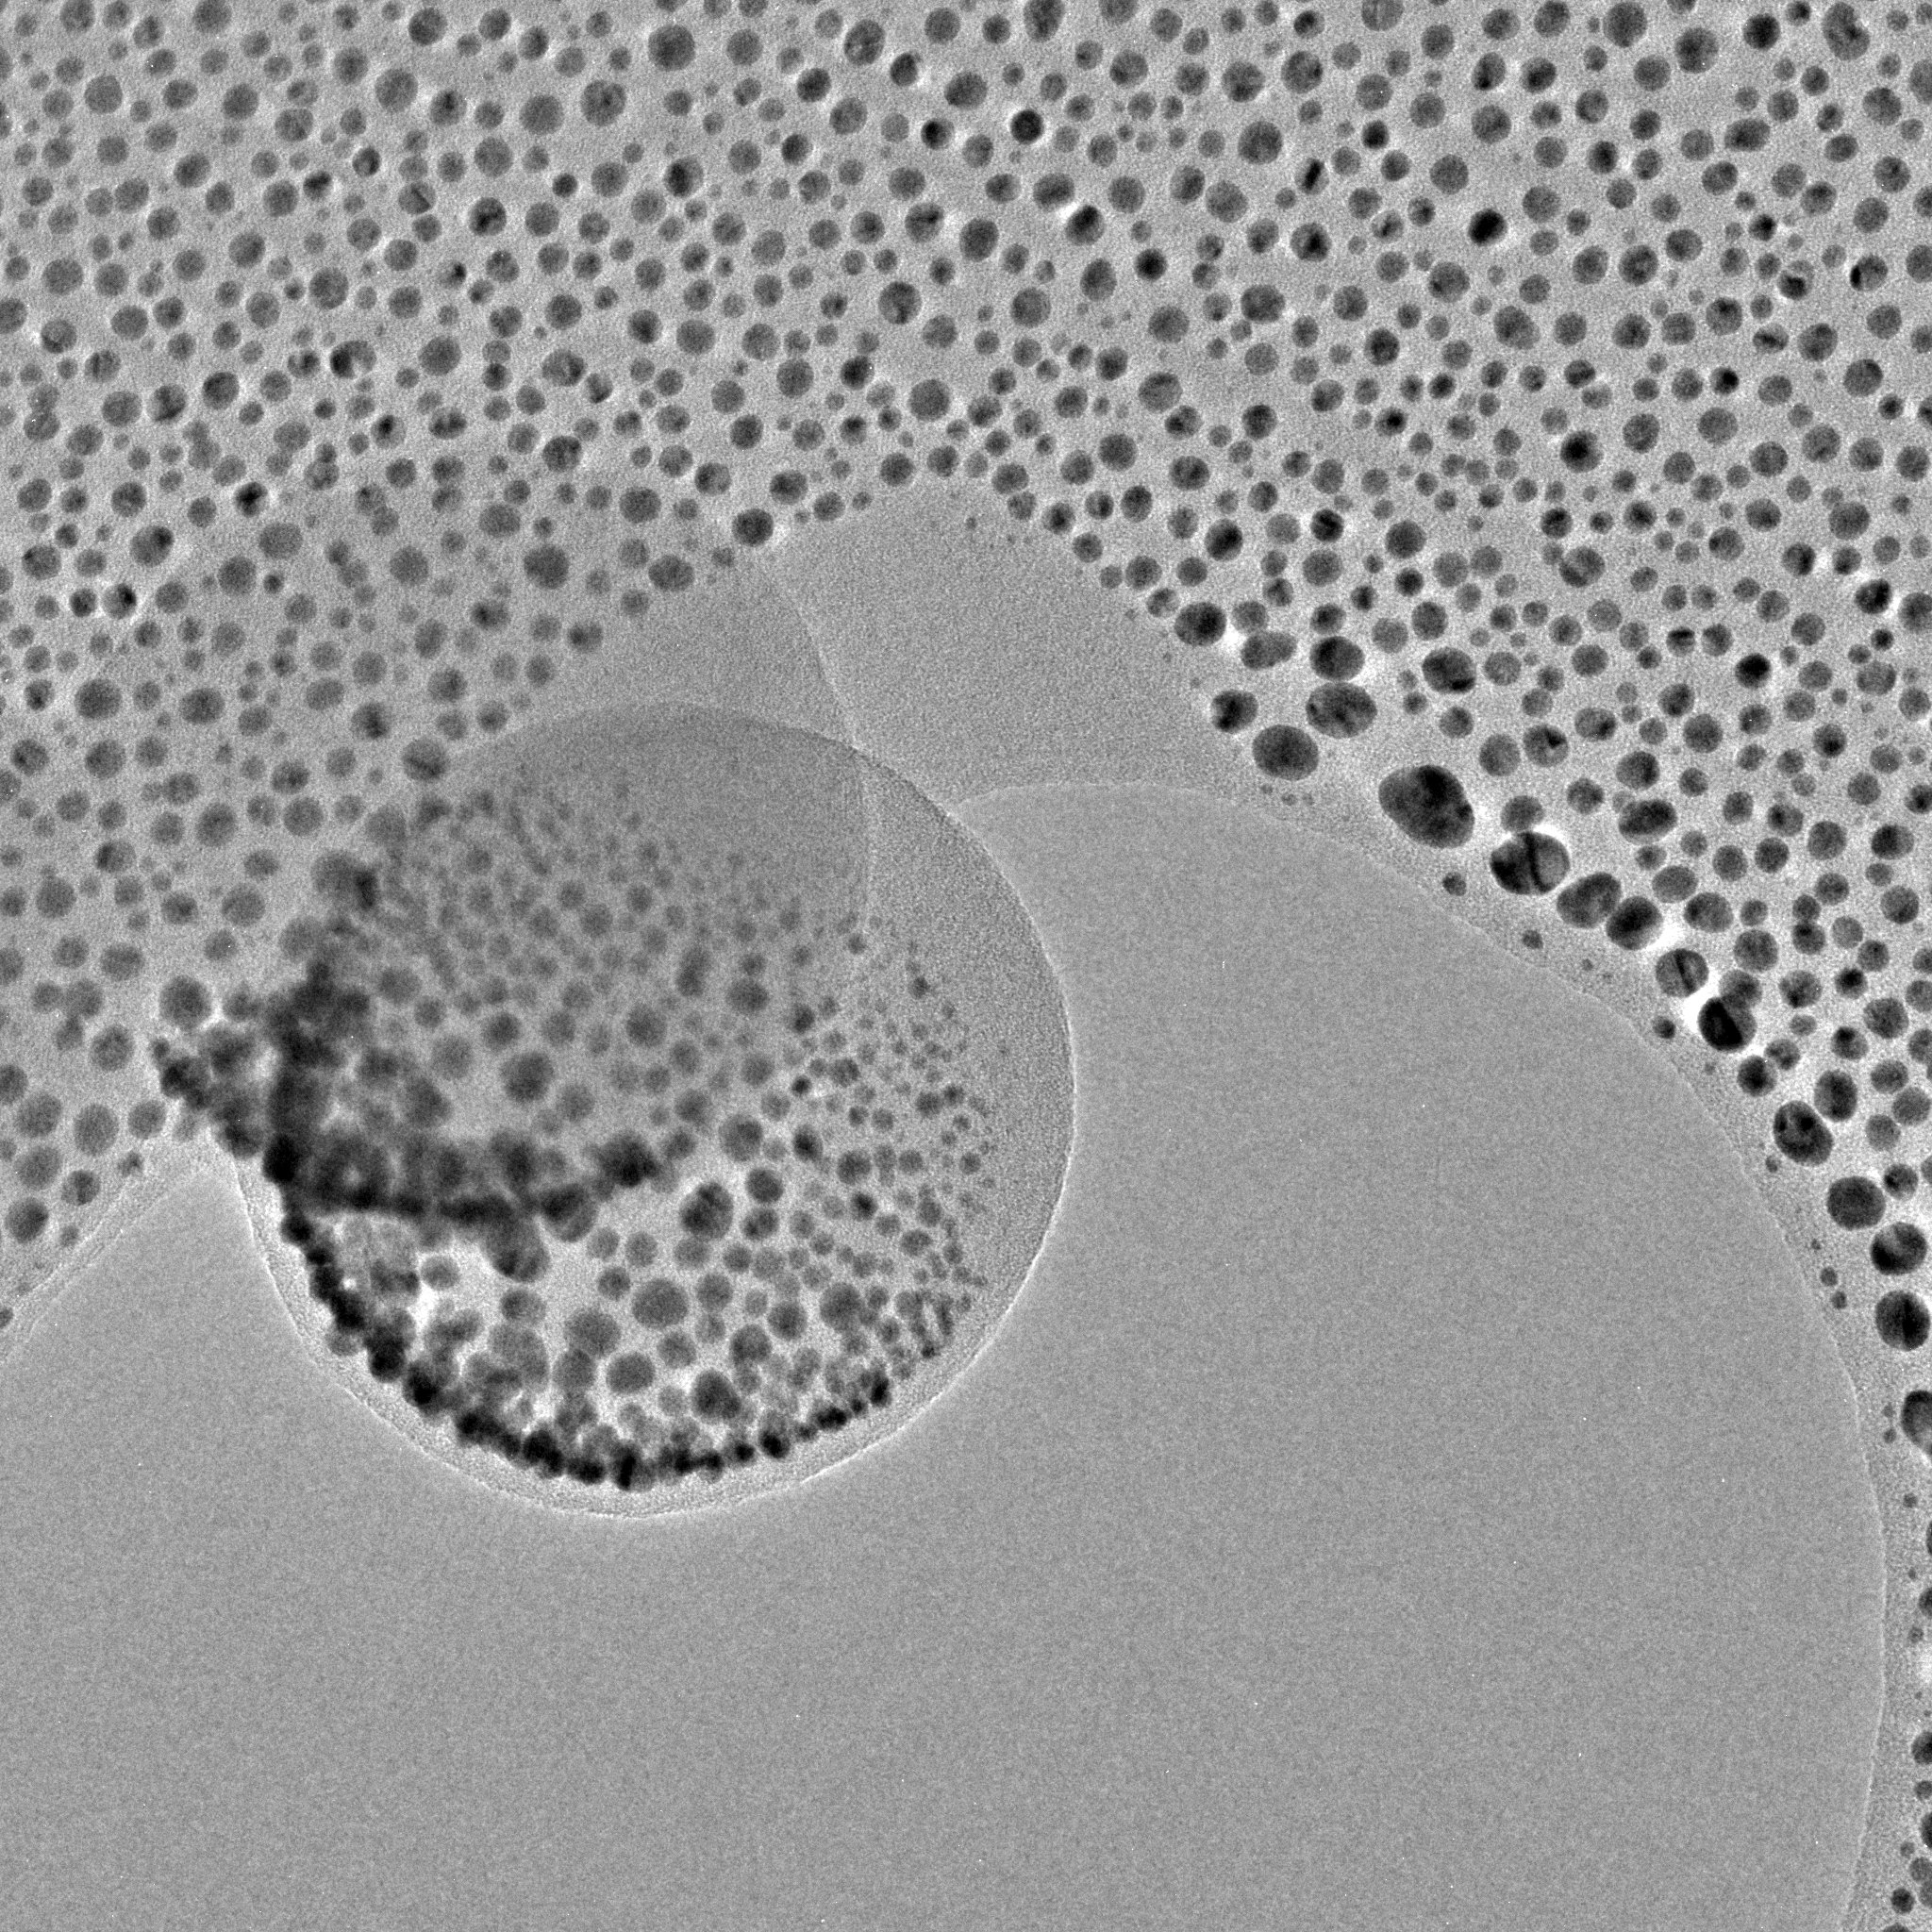
\includegraphics[width=\textwidth]{Grundlagen&Beugung/Lateckugel_Im_Fokus.jpg}
         \caption{Im Fokus}
         \label{SPFokus}
     \end{subfigure}
     \hfill
     \begin{subfigure}[b]{0.3\textwidth}
         \centering
         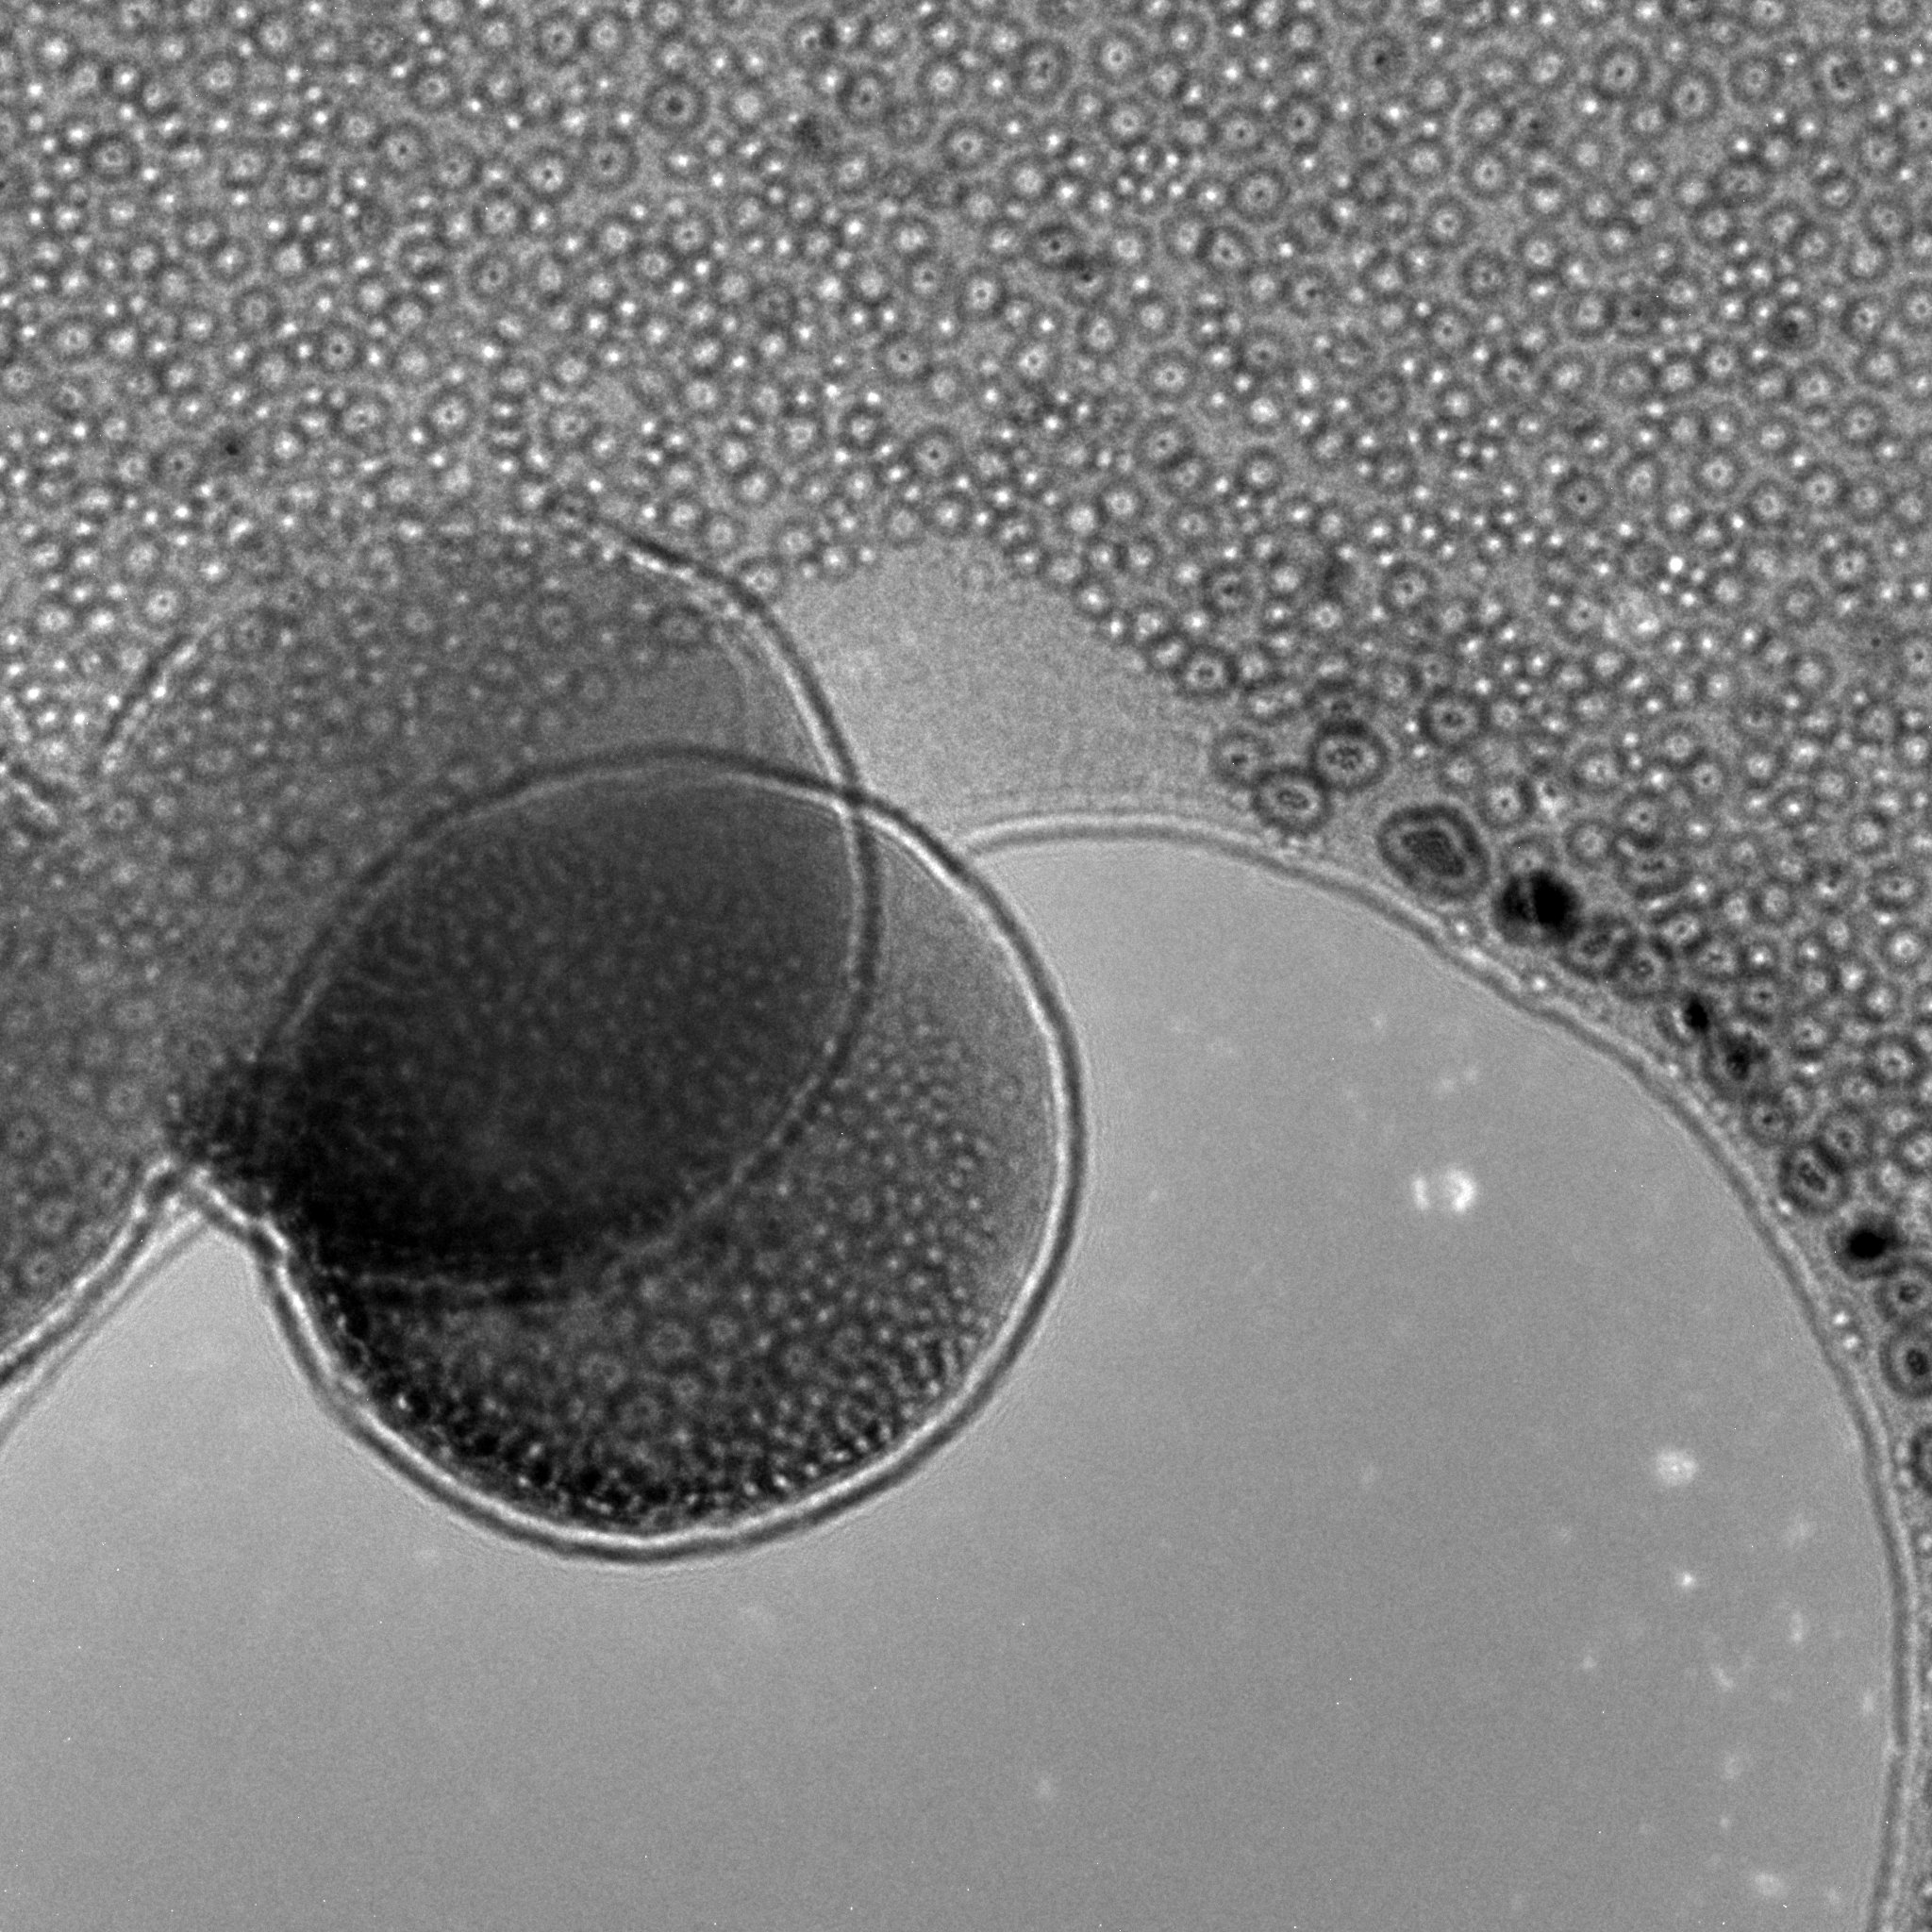
\includegraphics[width=\textwidth]{Grundlagen&Beugung/Latexkugeln_Im_Überfokus.jpg}
         \caption{Überfoku}
         \label{SPÜberfoku}
     \end{subfigure}
     \hfill
     \begin{subfigure}[b]{0.3\textwidth}
         \centering
         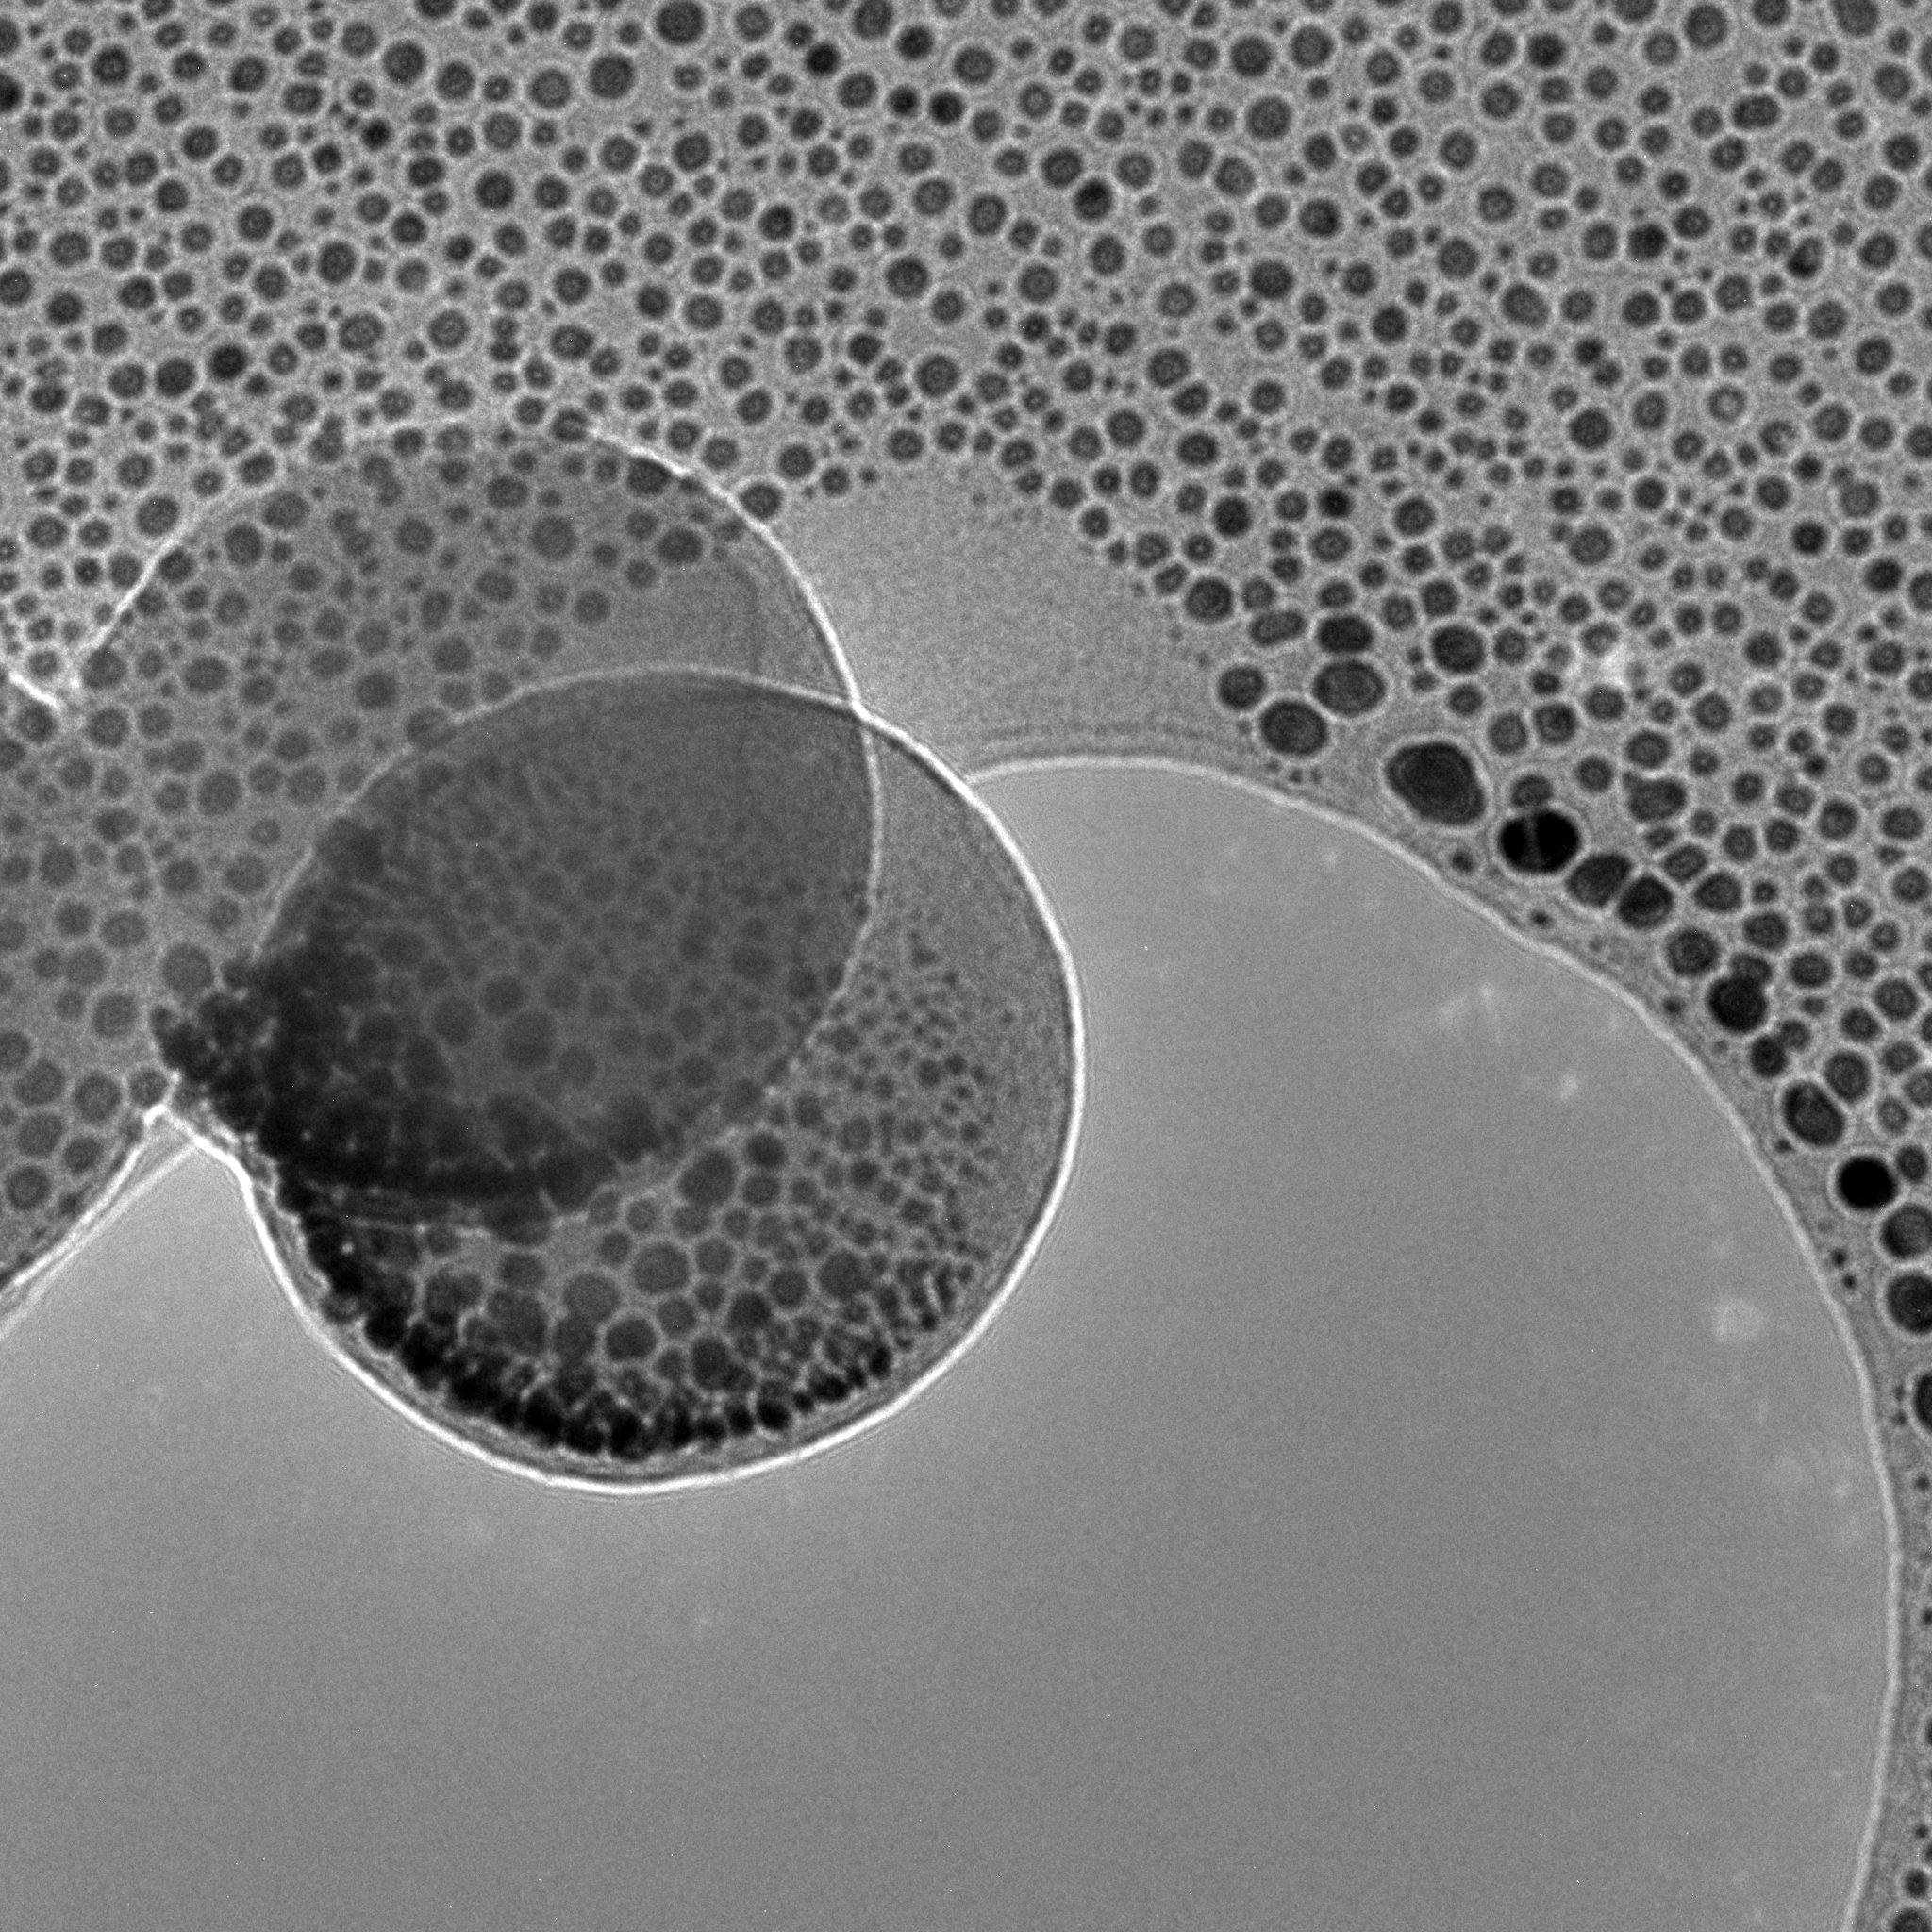
\includegraphics[width=\textwidth]{Grundlagen&Beugung/Latexkugeln_Im_Unterfokus.jpg}
         \caption{Unterfokus}
         \label{SPUnterfokus}
     \end{subfigure}
        \caption{TEM Aufnahmen eine Standardprobe, mit Kohlenstofffilm, Latex Kugeln und Goldpartikeln}
        \label{TEMStandardprobe}
\end{figure}

Am Bild im Fokus sind einige Elemente der Probe gut erkennbar: Es ist ein Kohlenstoff Film zu erkennen, dieser Film weist ein Loch an der Unteren kante der Aufnahme auf in dieser Region ist nur Vakuum abgebildet. Es sind außerdem die vergleichsweise großen Latex Kugeln und die kleineren Goldpartikel auf die auf dem Kohlenstoff Film aufgebracht sind Erkennbar. Hier wird der starke Kontrast zwischen den schweren Gold Partikeln und dem leichten Kohlestoff und Latex gut sichtbar. Der Kontrast zwischen Kohlestoff Film und Vakuum ist hingegen sehr schwach was auf einen guten Fokus hindeutet.\\
Der Überfokus entsteht, wenn die Probe entlang der optischen Achse leicht vor der Objektebene der Objektlinse positionirt ist. Bei der Aufnahme des Überfokus ist ein starker dunkler Kontrast am Rand/Saum des Kohlefilms erkennbar. Der Kontrast zwischen den Goldpartikeln und dem Kohlenstoff ist dagegen geringer als zuvor. \\
Im Unterfokus ist die Probe etwas hinter der Objektebene der Objektlinse positioniert, dabei ist ein Weißer Rand am der Kohlenstofffilm Kante zu erkennen, der Kontrast zwischen den Latex kugeln, den Goldpartikeln und dem Kohlenstofffilm ist jedoch immer noch ziemlich gut. In diesem Modus ist es leichter unterschiedliche Strukturen in der Probe auseinander zu halten und zu identifizieren.\\
Der helle und der dunkle Fresnel-Saum bei den defokussierten Abbildungen ergibt sich durch Interferenzerscheinungen. Entstehen durch die Beugung der Elektronenwelle an der Kohlenstoffkante.

\subsubsection{Gold-Cluster}
Die Gold Partikel wurden mit dem HRTEM in einer höheren Vergrößerung genauer angeschaut. Mit dieser Einstellung ist eine atomare Auflösung möglich, und erste Kristallstruktur Strukturen erkennbar. In der Aufnahme \cref{TEMGoldcluster} sind mehrerer Cluster zu erkennen, und auch die Orientierung und Anordnung der Goldatome innerhalb der einzelnen Cluster ist erkennbar. Die Cluster heben sich gegen den amorphe kohlestofffilm gut ab.

\begin{figure}[htbp]
 \centering
 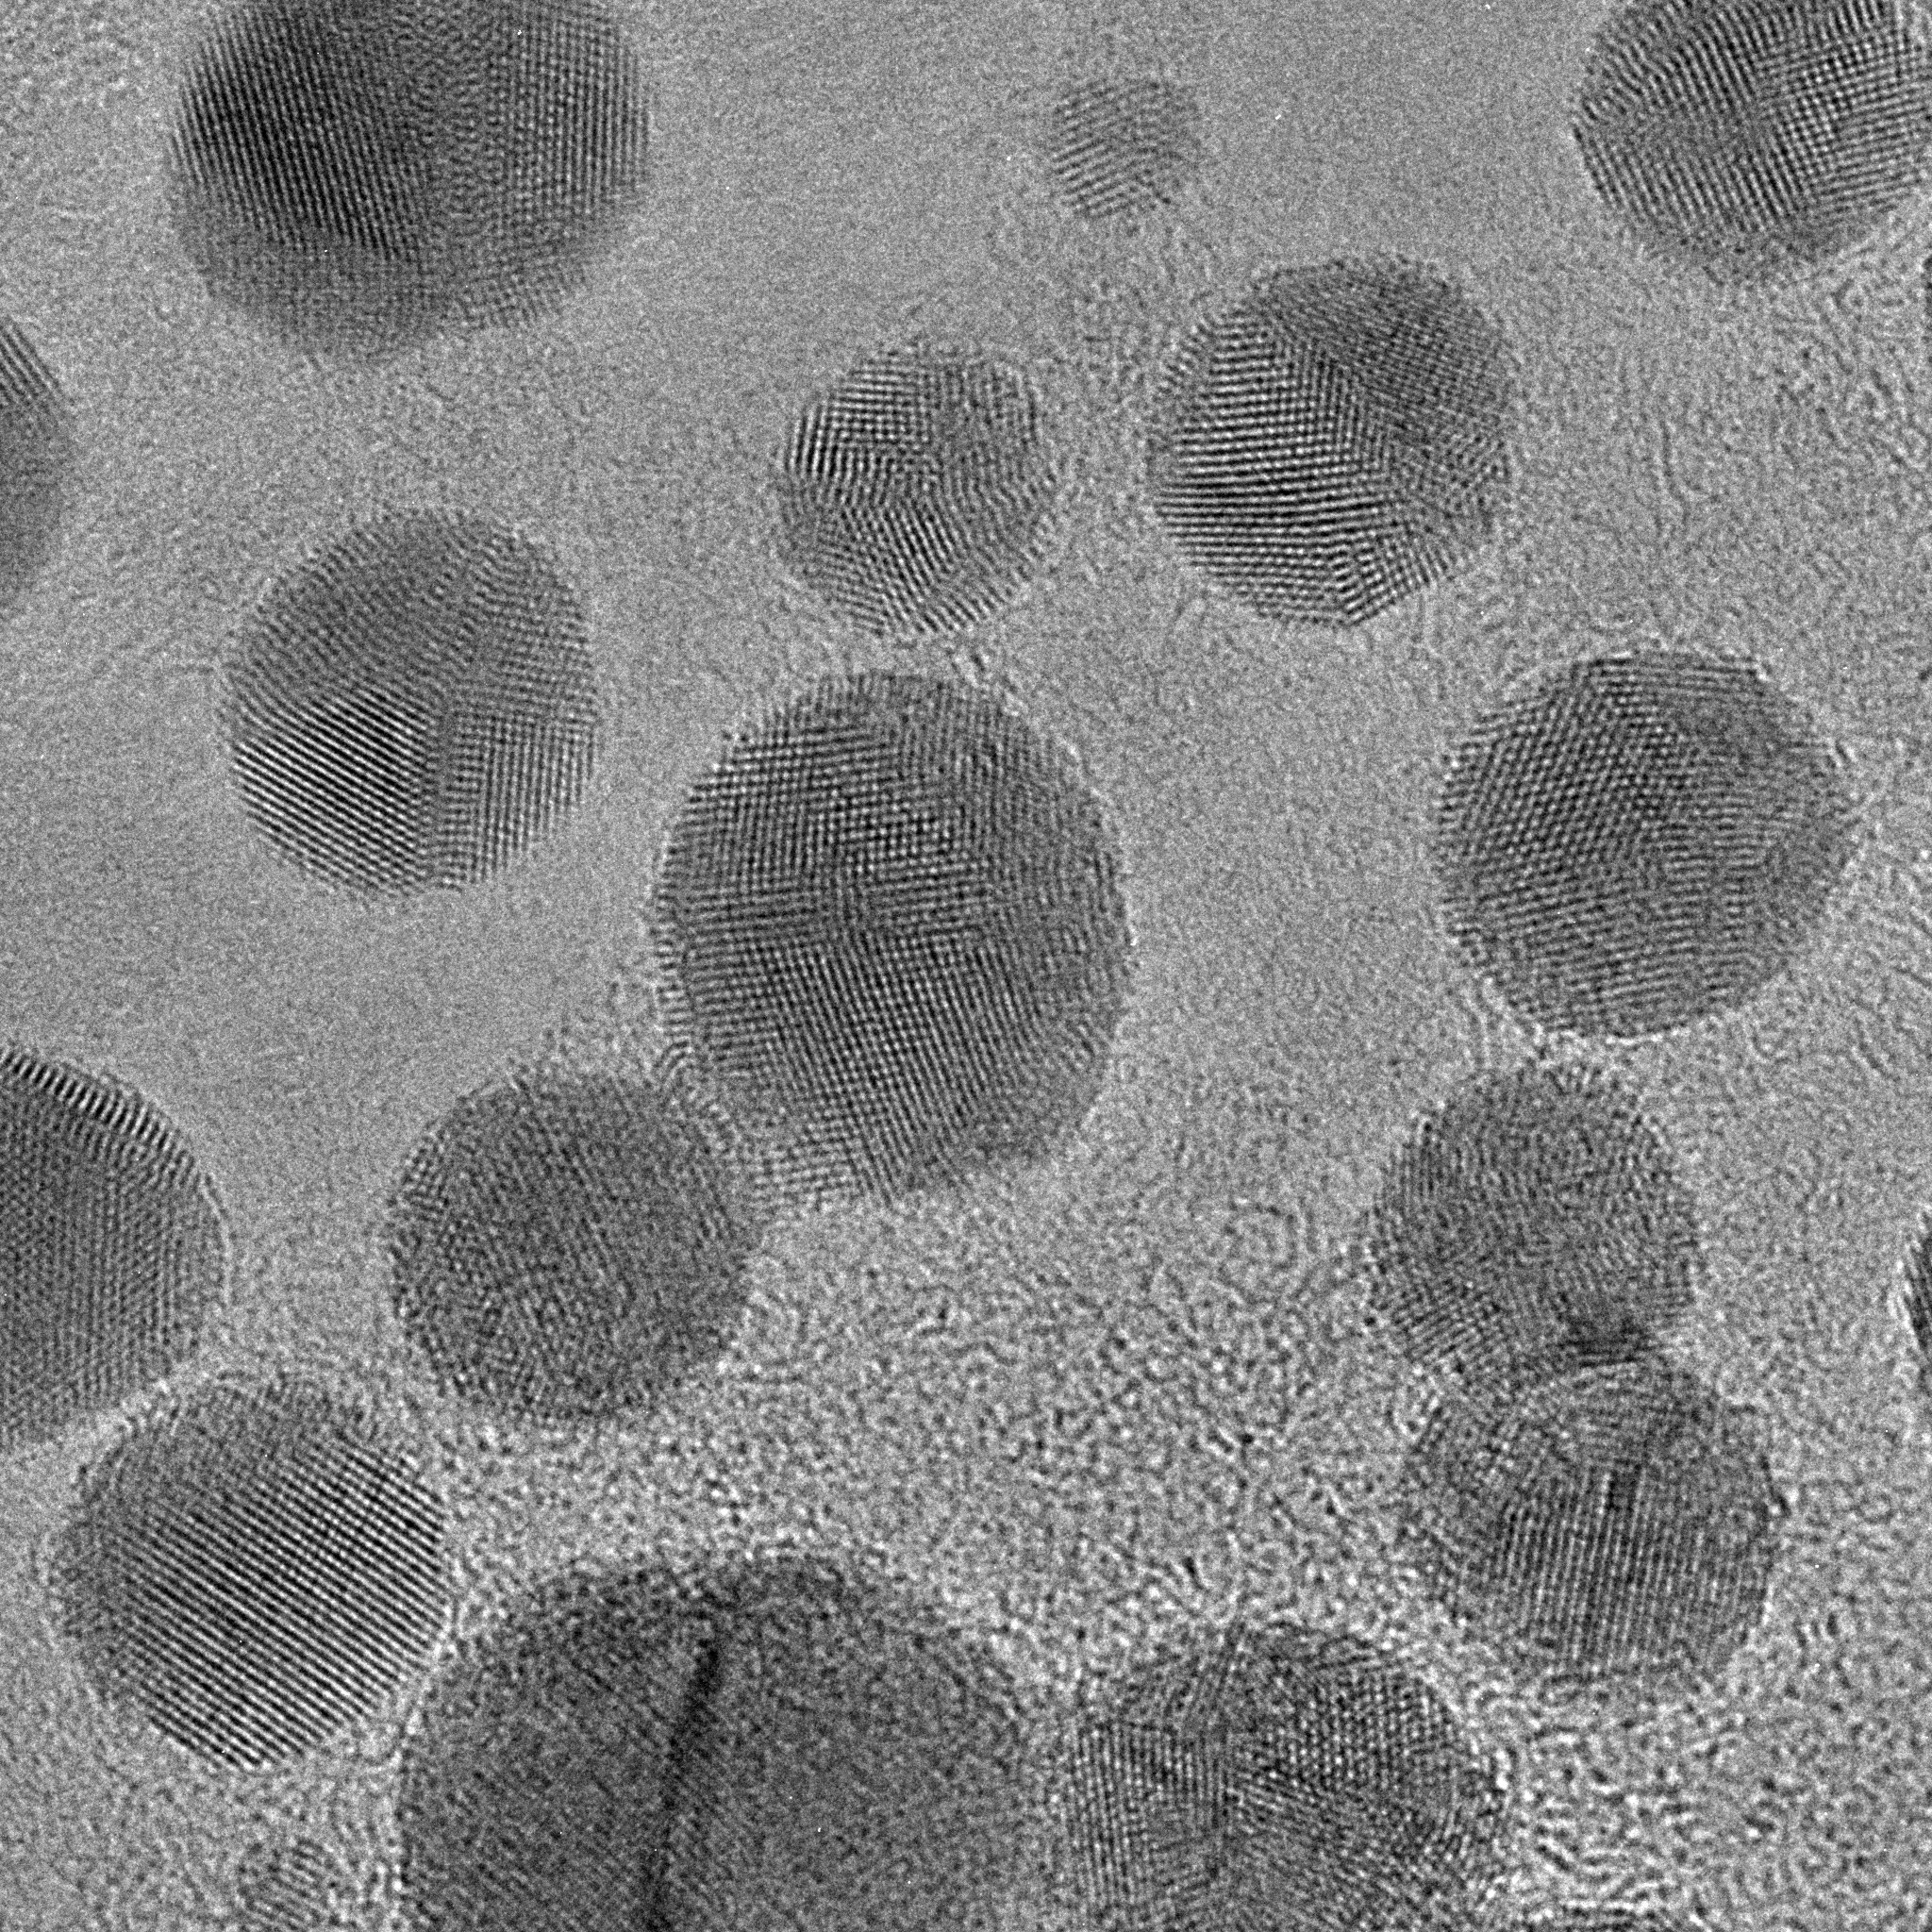
\includegraphics[width=0.7\textwidth]{Grundlagen&Beugung/Goldpartikel_im_leichten_ueberfokus.jpg}
 \caption[TEM Gold cluster]{TEM Aufnahme von Gold Cluster auf Kohlestofffilm}
 \label{TEMGoldcluster}
\end{figure}

\subsection{Aufnehmen von Beugungsbildern}
Um ein Beugungsbild aufzunehmen muss zuerst im Bildmodus des Mikroskops eine adäquate stelle auf der Probe identifiziert werden und die ins Zentrum des Leuchtschirmes verfahren werden. Um ins Beugungsbild zu wechseln muss der „Diffraction“ Knopf am Steuer Panel gedruckt werden. Dies Verändert die Leistung der „Diffraction lense“ (DL) und „Projection lense“ (PL) linsen so dass ein Beugungsbild abgebildet wird. Um die CCD Kamera vor zu starker Einstrahlung zu schützen muss vor dem hochklappen des Leuchtschirm ein „Beam Stopper“ in den null strahl verfahren werden. Zusätzlich können SA Blende eingebracht werden, in diesen versuch wurde eine 10 Mikrometer und 40 Mikrometer Blende verwendet. Das Beugungsbild kann nun nach dem hochklappen des Leuchtschirm und ausfahren der CCD Kamera aufgenommen werden.

\subsubsection{Beugungsbilder der Au Probe mit verschiedenen Blenden}

Zuerst wurde ein Bild mit einem SA Blende von 10 Mikrometer aufgenommen, das Beugungsbild ist auf einem amorphen kohlenstofffilm Teil der Probe aufgenommen. Die Beleuchtungszeit der CCD Kamera betrug 8 Sekunden (siehe Abbildung \cref{AU10um} ).\\
Die dieser Blenden Größe sind vor allem vereinzelte Punkte zu erkennen, diese bilden auch schon Andeutungen von ringen. Beugungsringe entstehen bei einer polykristallinen Probe mit unterschiedlichen kristallographischen Orientierungen. Jedoch kann, wenn nur einige wenige Kristall Orientierungen beleuchtet werde, sich die beleuchtungsringe nicht vollständig schließen.

\begin{figure}[htbp]
 \centering
 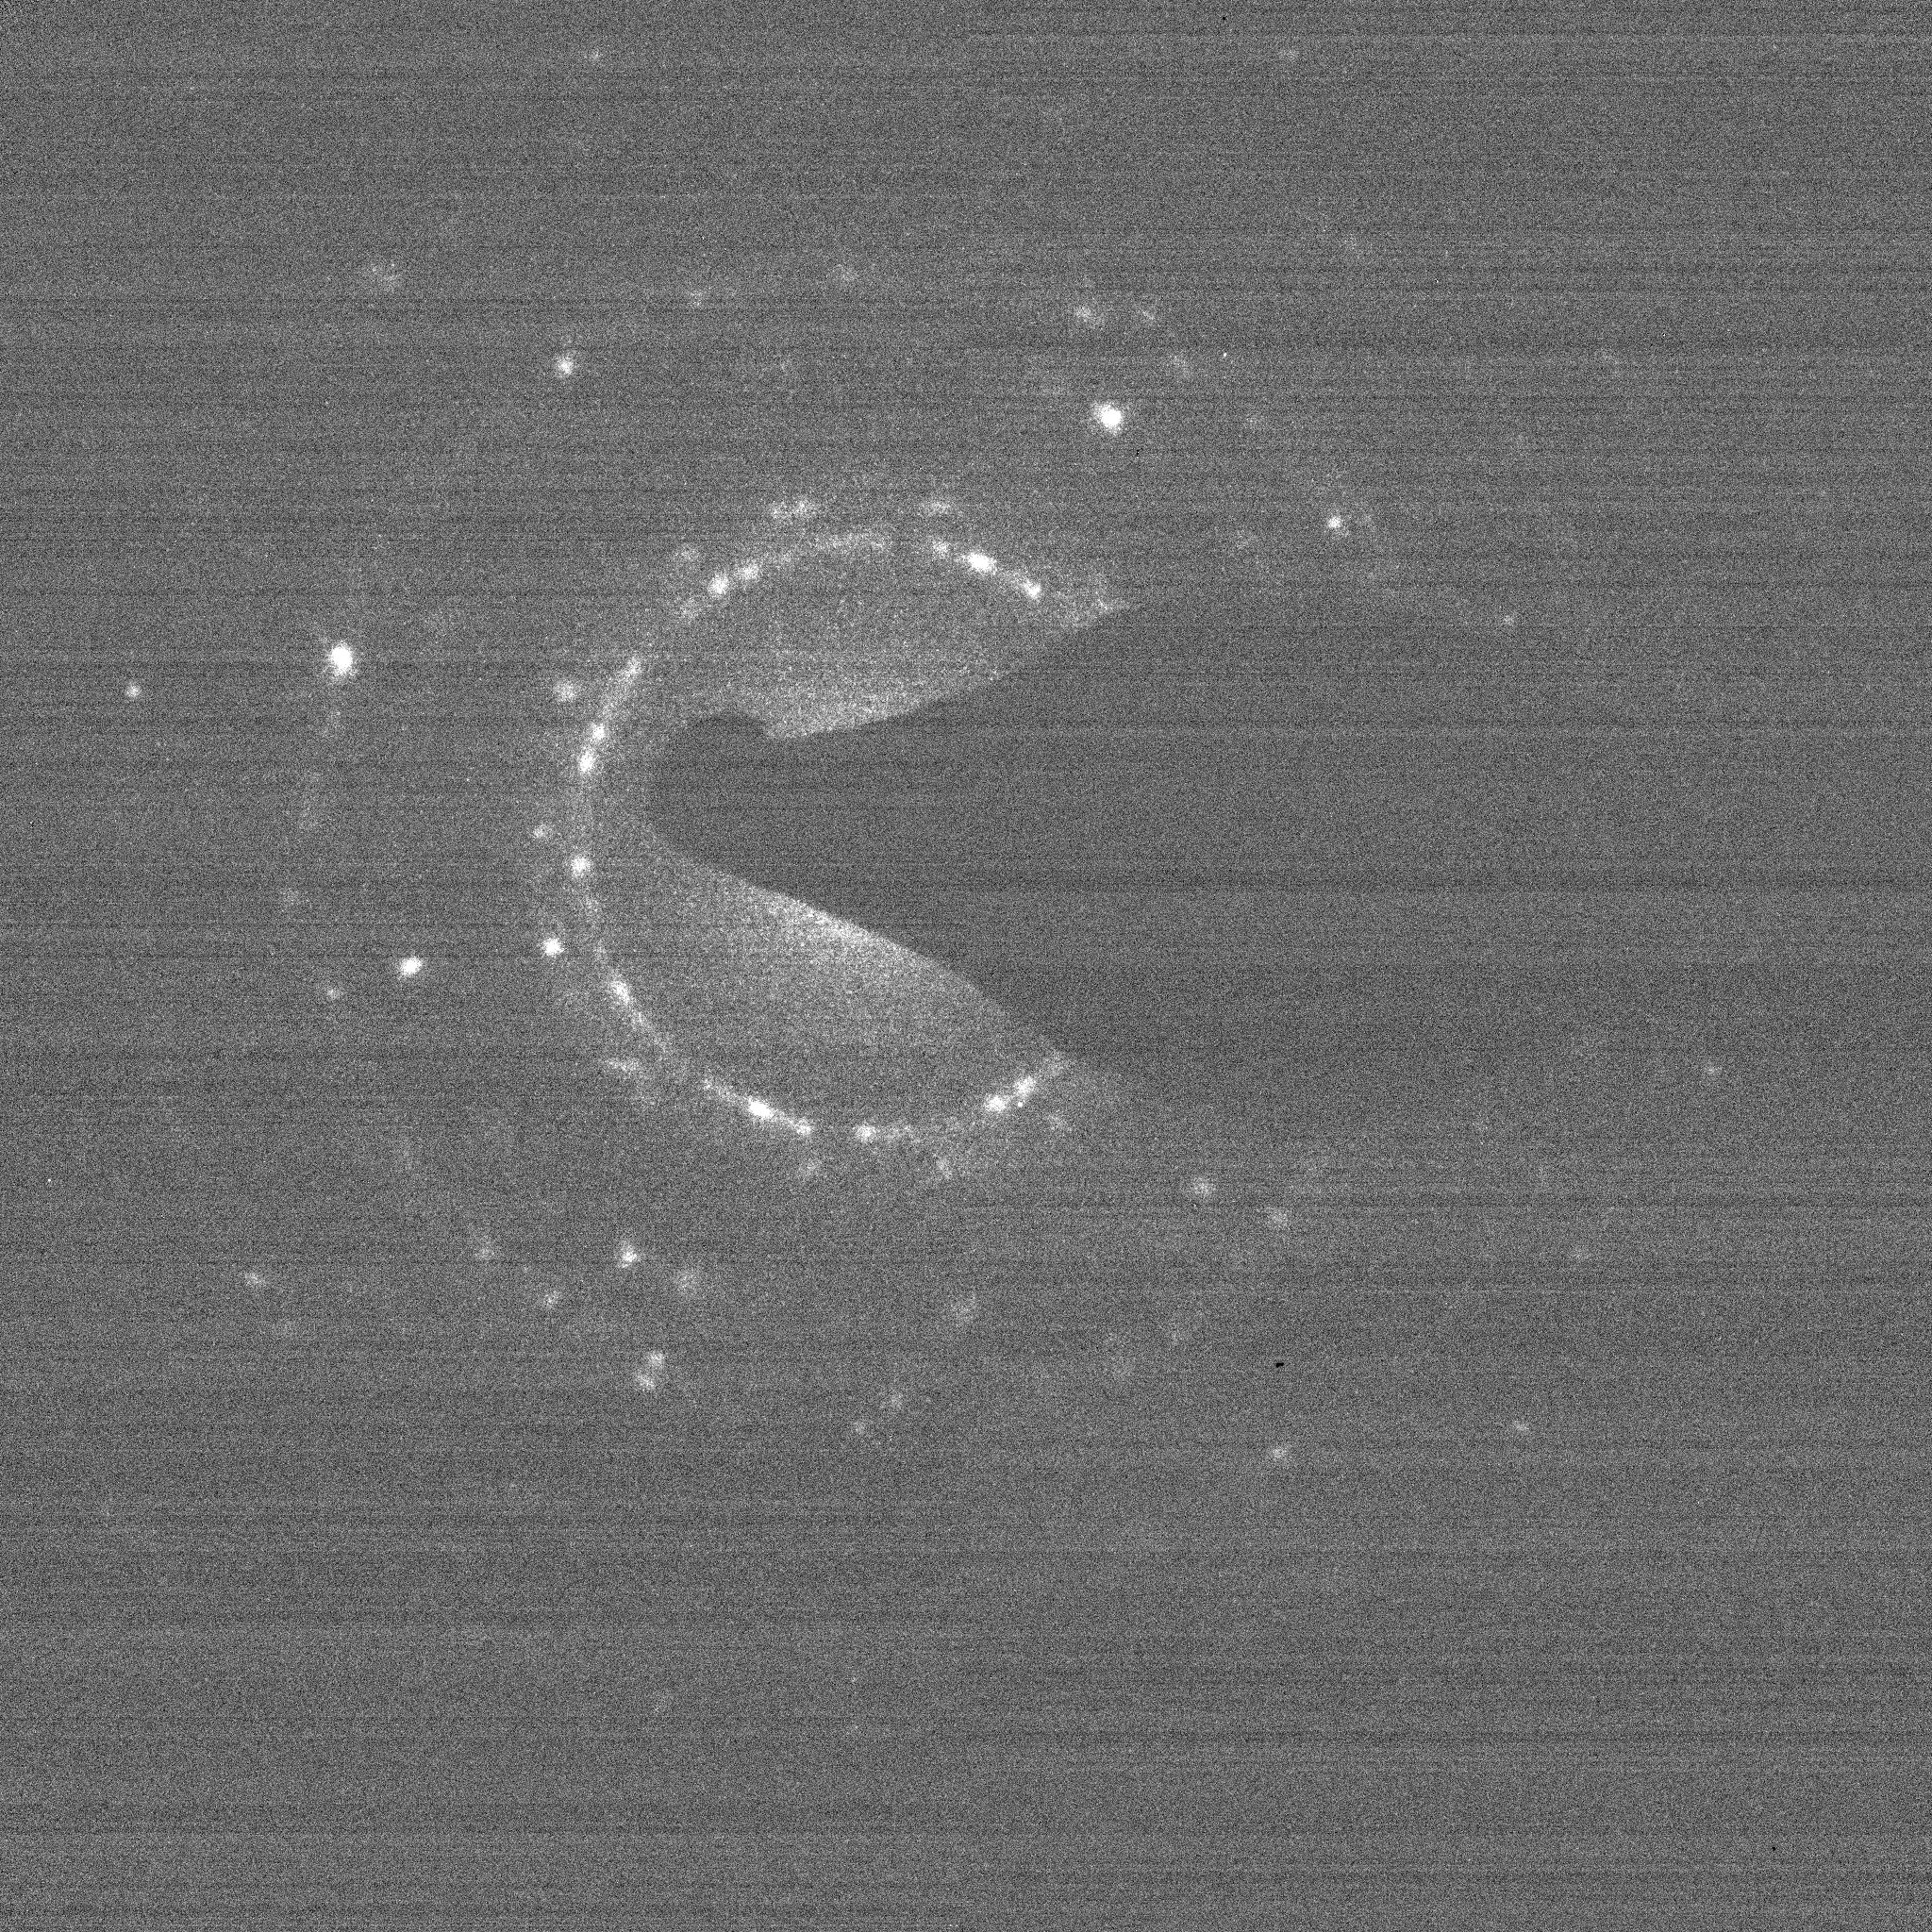
\includegraphics[width=0.7\textwidth]{Grundlagen&Beugung/Blende_10_Beugung_8sec.jpg}
 \caption[Beugungsbild Au 10µm Blede]{TEM Beugungsbild aufnahme von Au Cluster mit 10µm SA-Blende und 8 sec Beleuchtungszeit}
 \label{AU10um}
\end{figure}

Anschließend wurde ein Beugungsbild mit einer SA Blende von 40 Mikrometer aufgenommen. Die Beleuchtungszeit betrug 4 Sekunden (siehe Abbildung \cref{AU40um}). Hierbei sind die ringförmigen Muster abgebildet, einzelne Punkte sind dennoch gut erkennbar.

\begin{figure}[htbp]
 \centering
 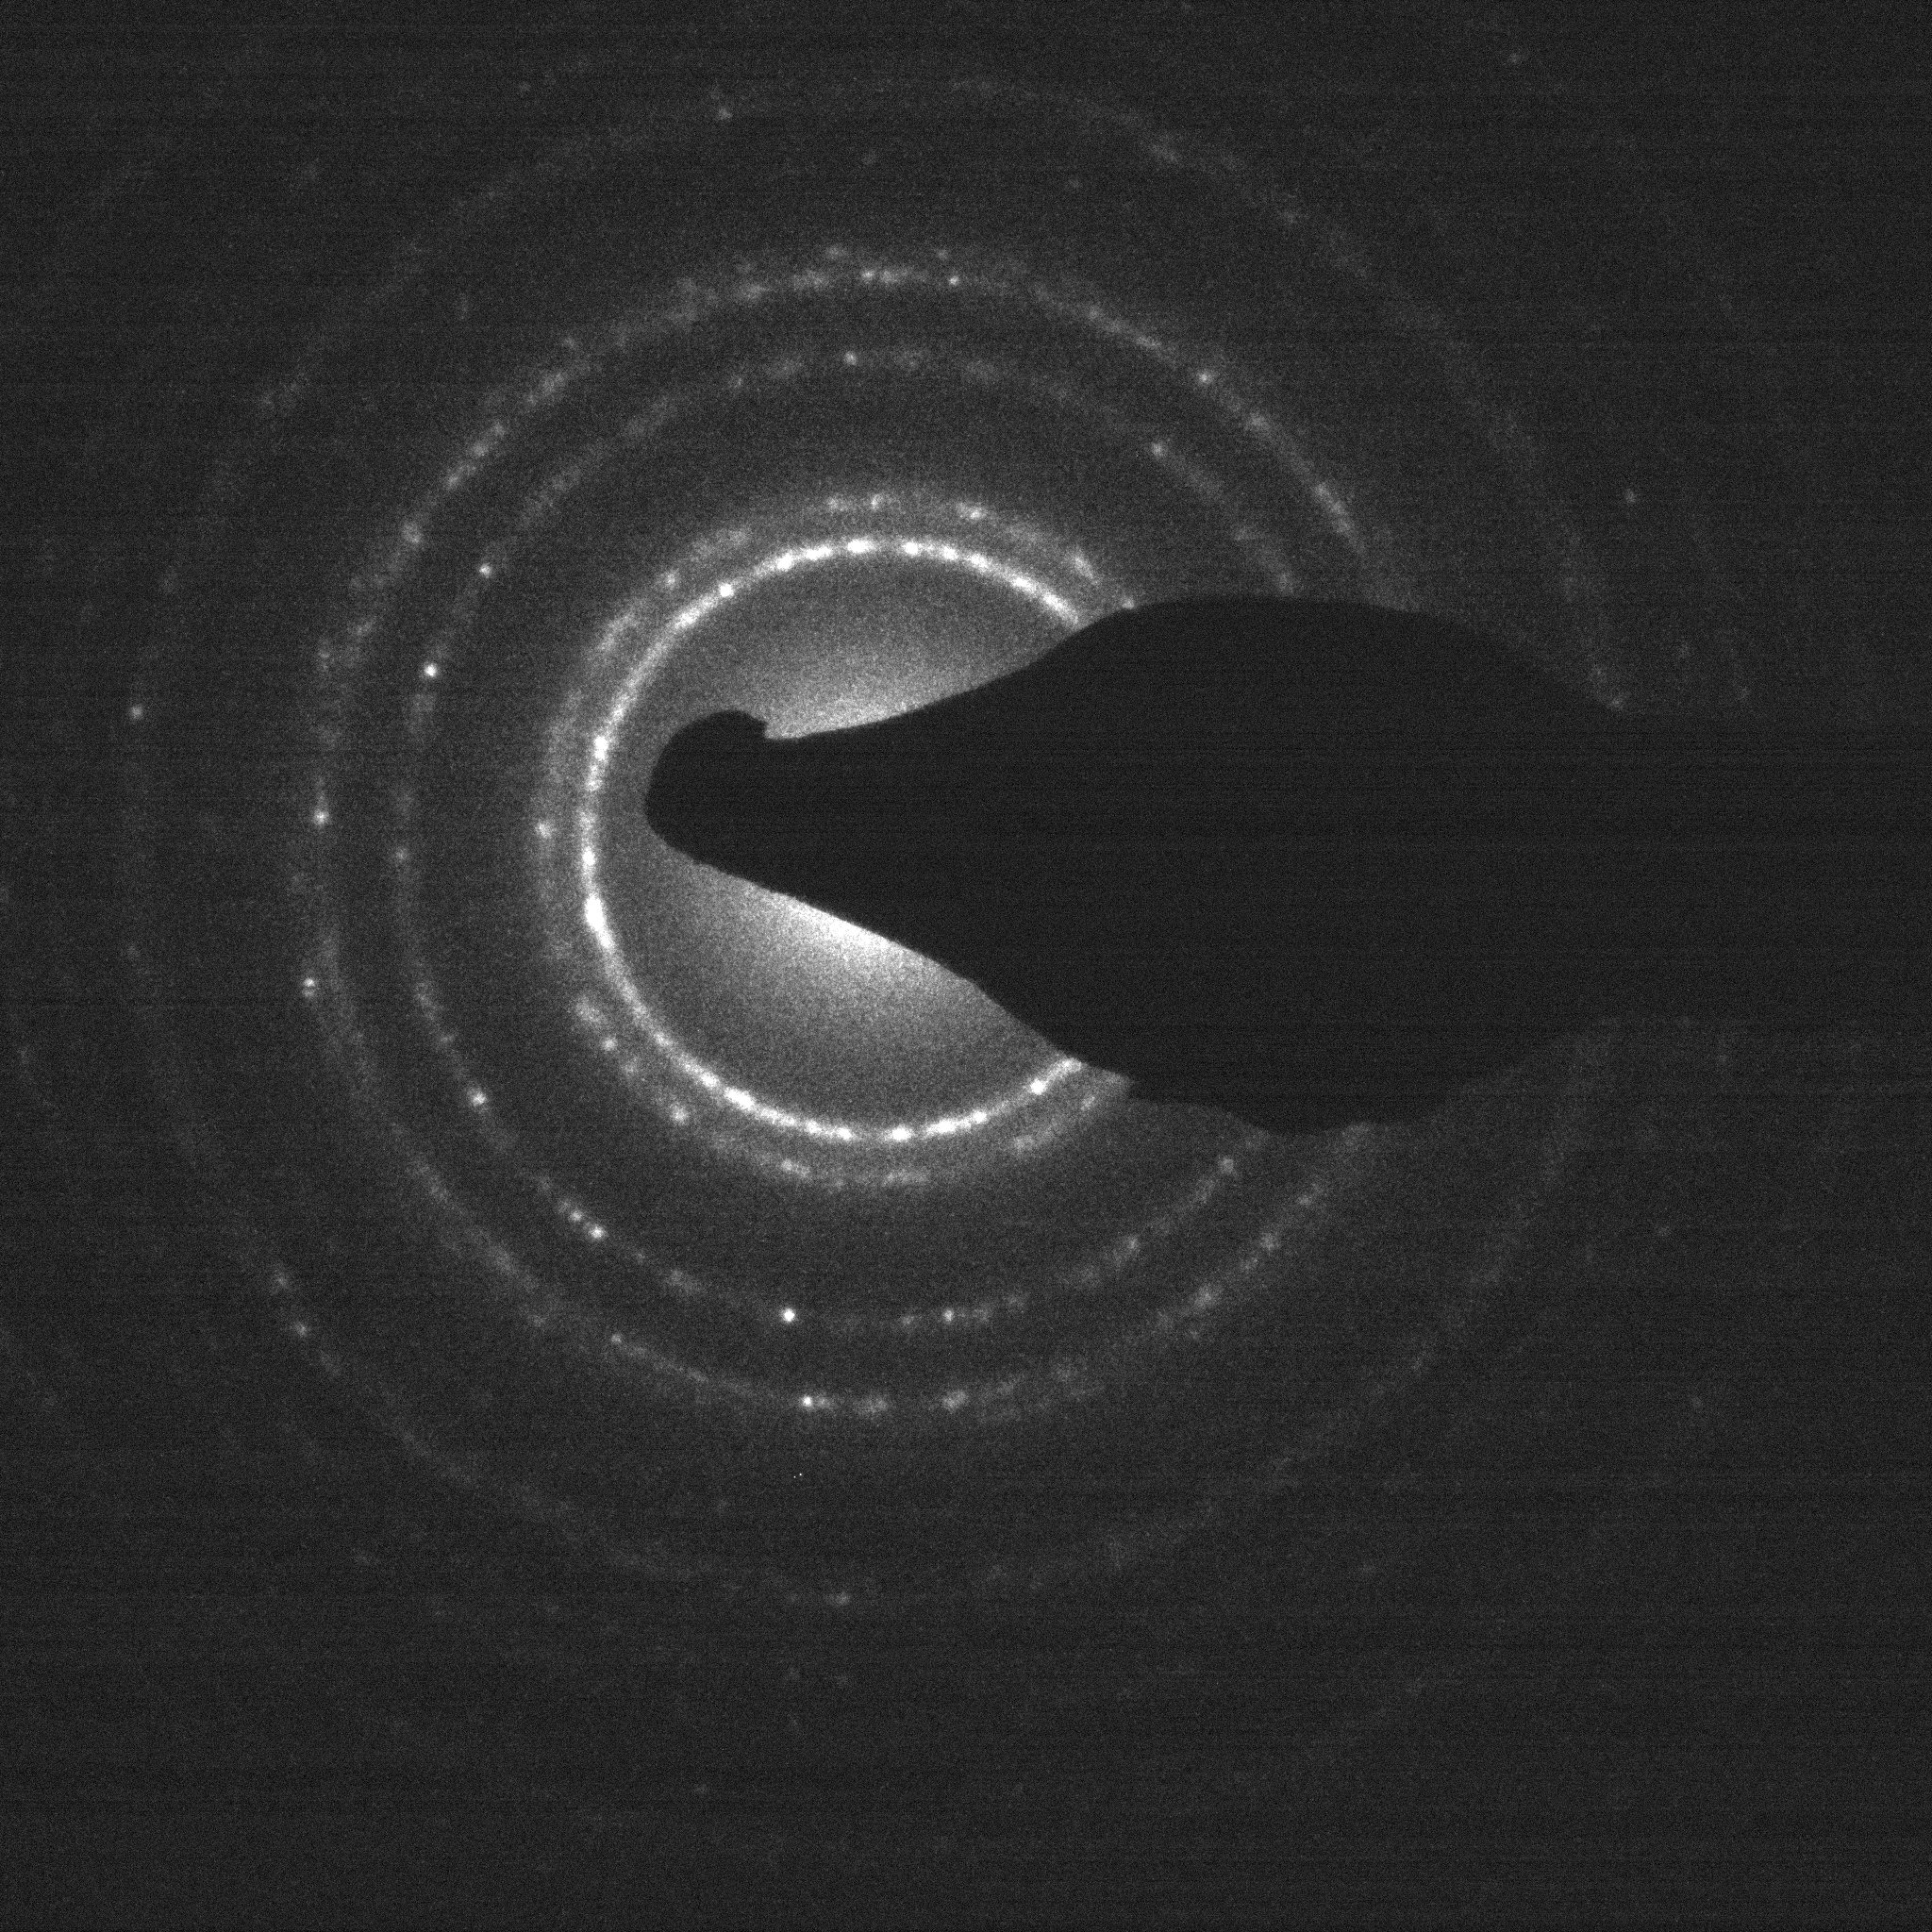
\includegraphics[width=0.7\textwidth]{Grundlagen&Beugung/Blende_40_Beugung_4sec.jpg}
 \caption[Beugungsbild Au 40µm Blede]{TEM Beugungsbild aufnahme von Au Cluster mit 40µm SA-Blende und 4 sec Beleuchtungszeit}
 \label{AU40um}
\end{figure}

\subsection{Hell-/ Dunkelfeld aufnehmen}
Die Standardprobe und insbesondere eine Latex Kugel wurde sich zusätzlich zum „Brightfield“, in dem vor allem die Streuabsorption der Probe abgebildet wird, auch das „Darkfield“ angeschaut. Beim Darkfield wird vor allem die Streuung an der Probe abgebildet.\\ 
Um ein Darkfield Aufnahme zu erlangen wird gibt es Zwei Möglichkeiten die im Laufe des Versuchs auch beide ausprobiert wurden. Das „dirty Dakfield“ und das „Centered Darkfield“.
\subsubsection{Dirtk darkfield}
Beim Dirty darkfield wird im Beugungsbild eine Beugungsblende vom Zentrum weg zu einem brechungsreflex verfahren. Wenn anschließend ins Bildmodus zurück gewechselt wird sind dann nur Elektronen aus diesem Brechungsreflex zu sehn. Es kann dann ein so genanntes Darkfield Bild aufgenommen werden. Hierbei kann es zu Bildfehlern kommen so das diese Methode nicht optimal ist.

\subsubsection{Centered Darkfield}
Bei Centered Darkfield, wird anstatt die Blende zu verfahren der Elektronenstrahl so verkippt das der gewünschte Reflex durch das Loch in der zentrierten Beugungsblende fällt. Dies hat denselben Effekt wie bei Dirty darkfild aber ohne die Bildfehler, und kann so einen Duknkelfeld Bild aufgenommen werden.

\subsubsection{Standard Probe Hell/Dunkel Feld Aufnahmen}
Bei der Hellfeld Aufnahme der Standard Probe sind die Goldpratikel recht gut durch ihren hohen dunklen Kontrast zu erkennen. Dies last sich durch den schweren Gold Atome erklären die eine Größe Streuung verursachen. Die Latex Kugeln sind ebenfalls gut erkennbar. Der Kohlenstofffilm zeigt jedoch nur einen sehr geringen Kontrast auf.\\
Bei der Centerd Darkfield Aufnahme sind vor allem die Goldpartikel mit einem Besonders guten Kontrast zu erkennen da sie sich Hell vom Dunklen Hintergrund abheben. Nicht alle Goldcluster sind jedoch gleichermaßen gut sichtbar. Dies wird durch die unterschiedliche Orientierung der Kristallstrukturen der jeweiligen Cluster zu erklären. Die Latex Kugeln sind auch in diesem Modus noch erkennbar. Der Kohlefilm hingegen ist quasi nicht sichtbar. 

\begin{figure}
     \centering
     \begin{subfigure}[b]{0.49\textwidth}
         \centering
         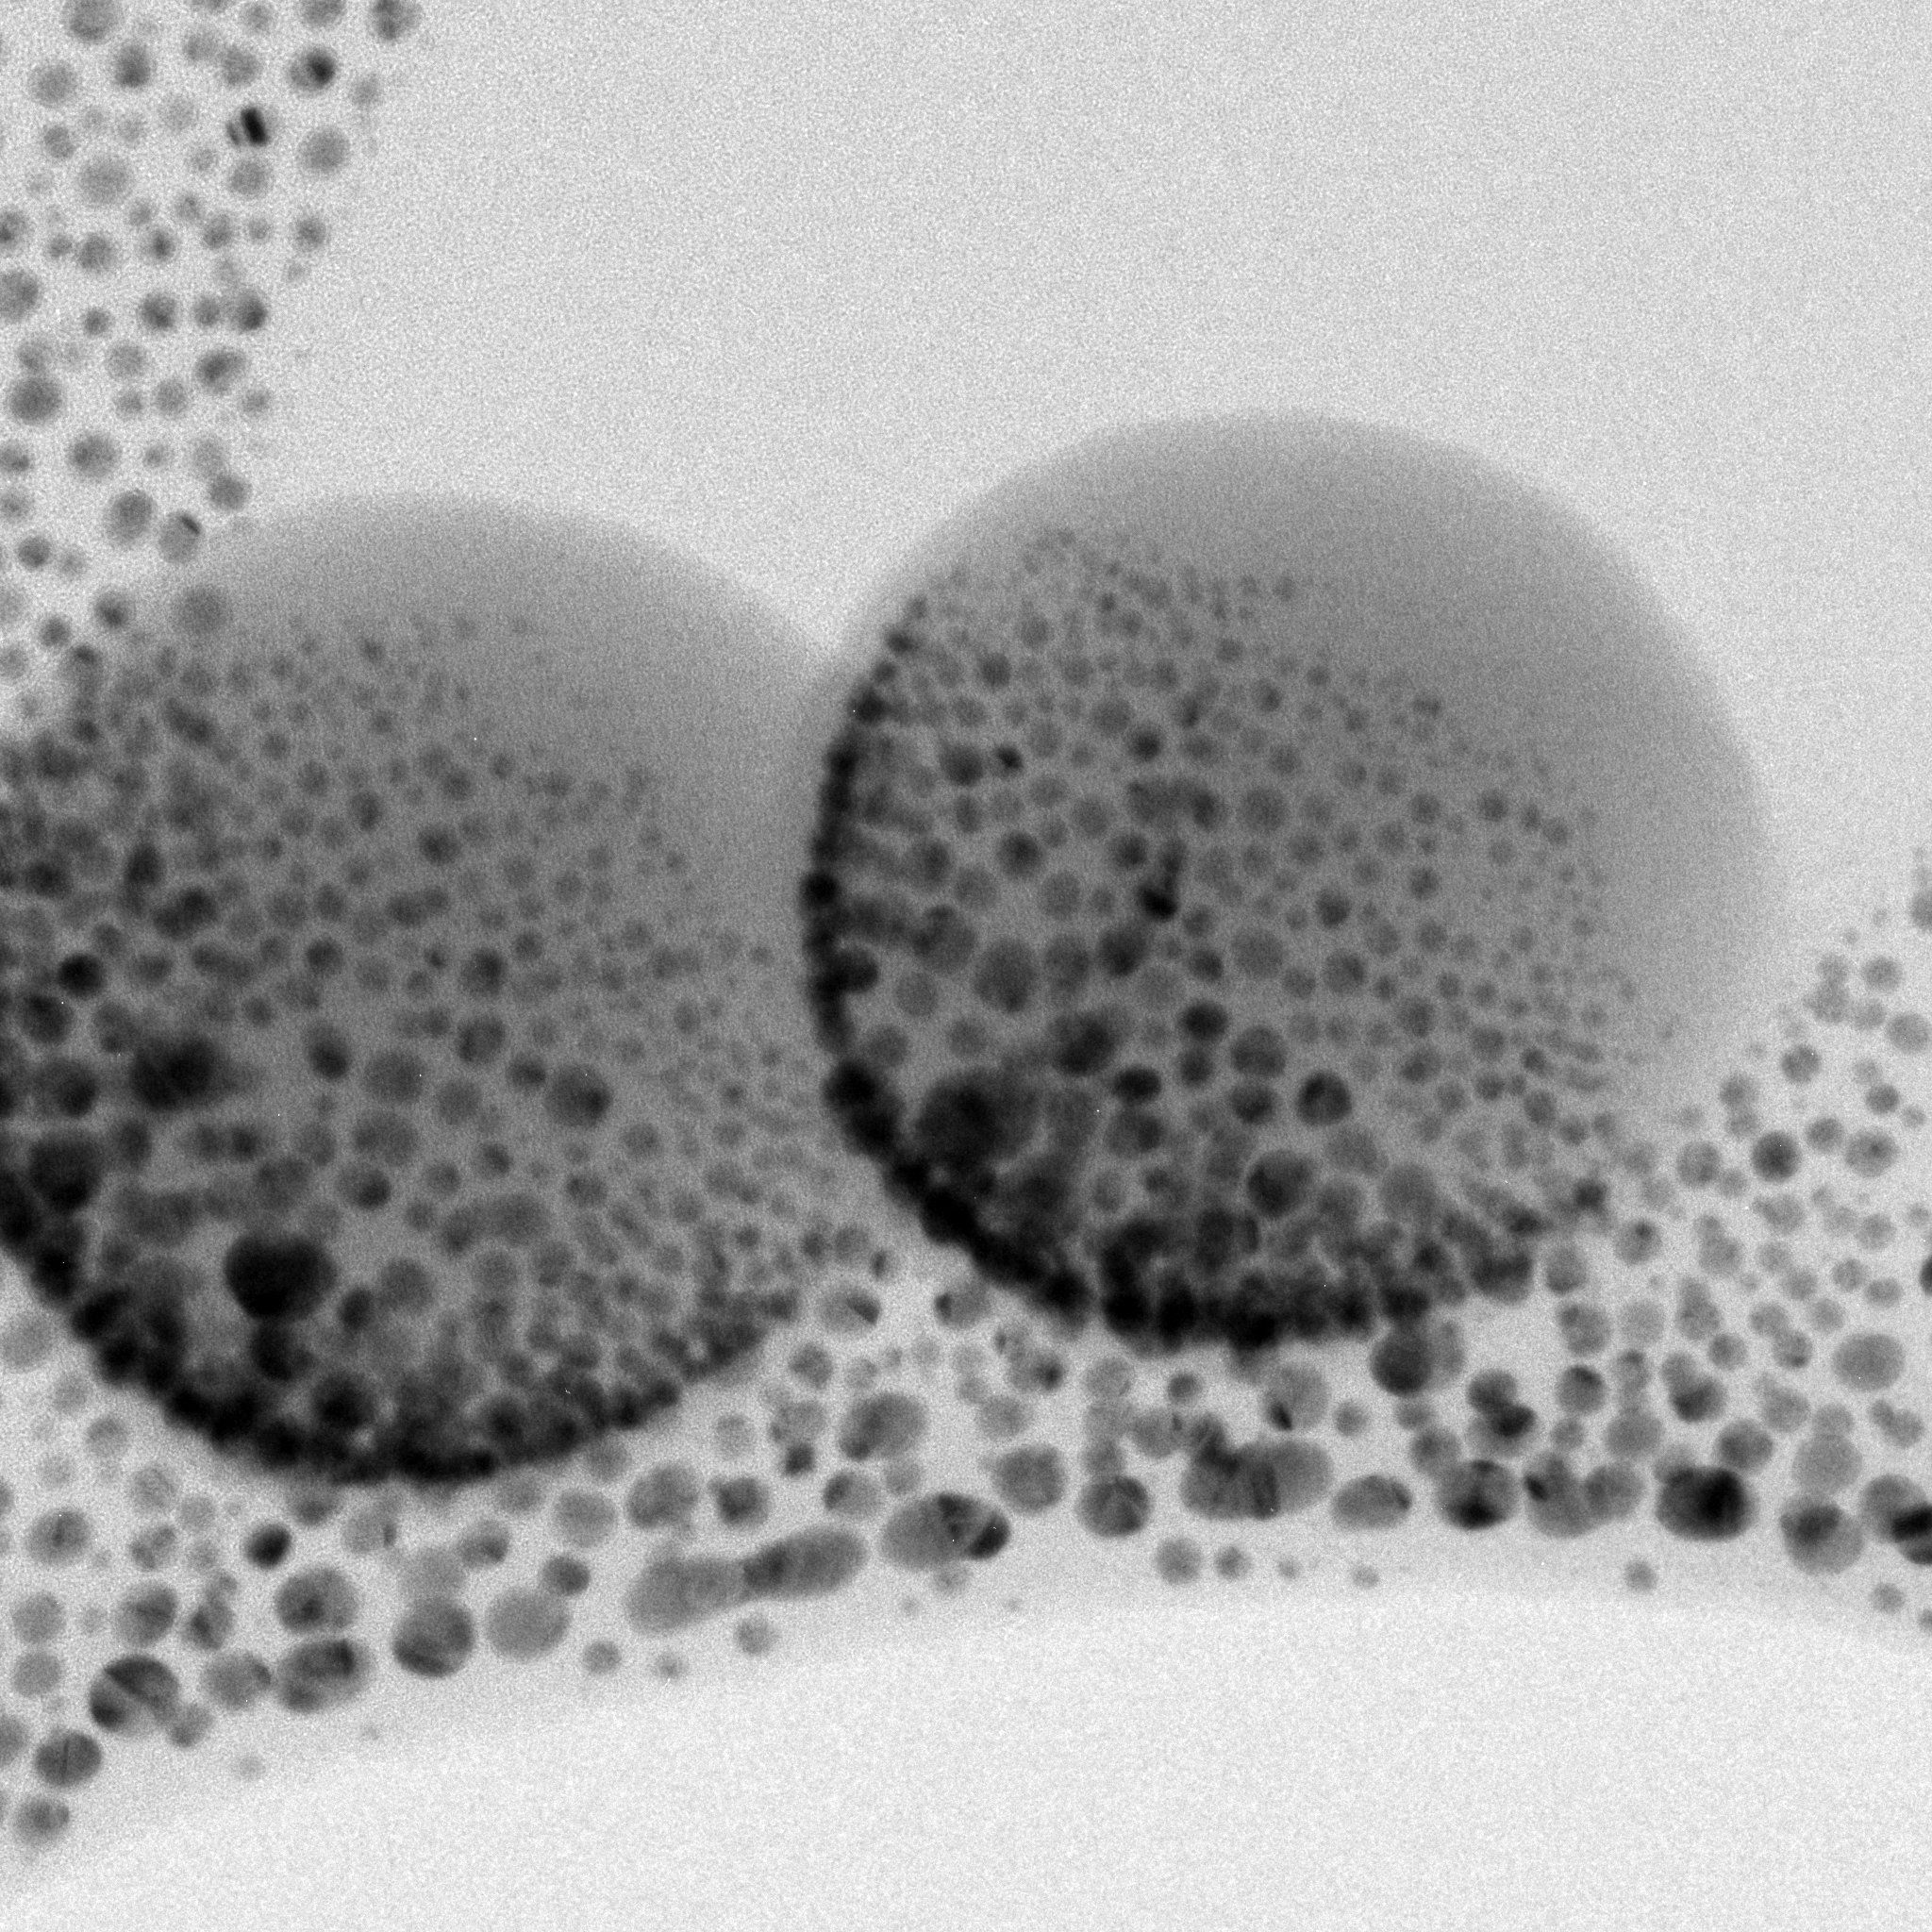
\includegraphics[width=\textwidth]{Grundlagen&Beugung/Goldpartukel_1sec_brightfeeld2.jpg}
         \caption{Brightfield}
         \label{SPBF}
     \end{subfigure}
     \hfill
     \begin{subfigure}[b]{0.49\textwidth}
         \centering
         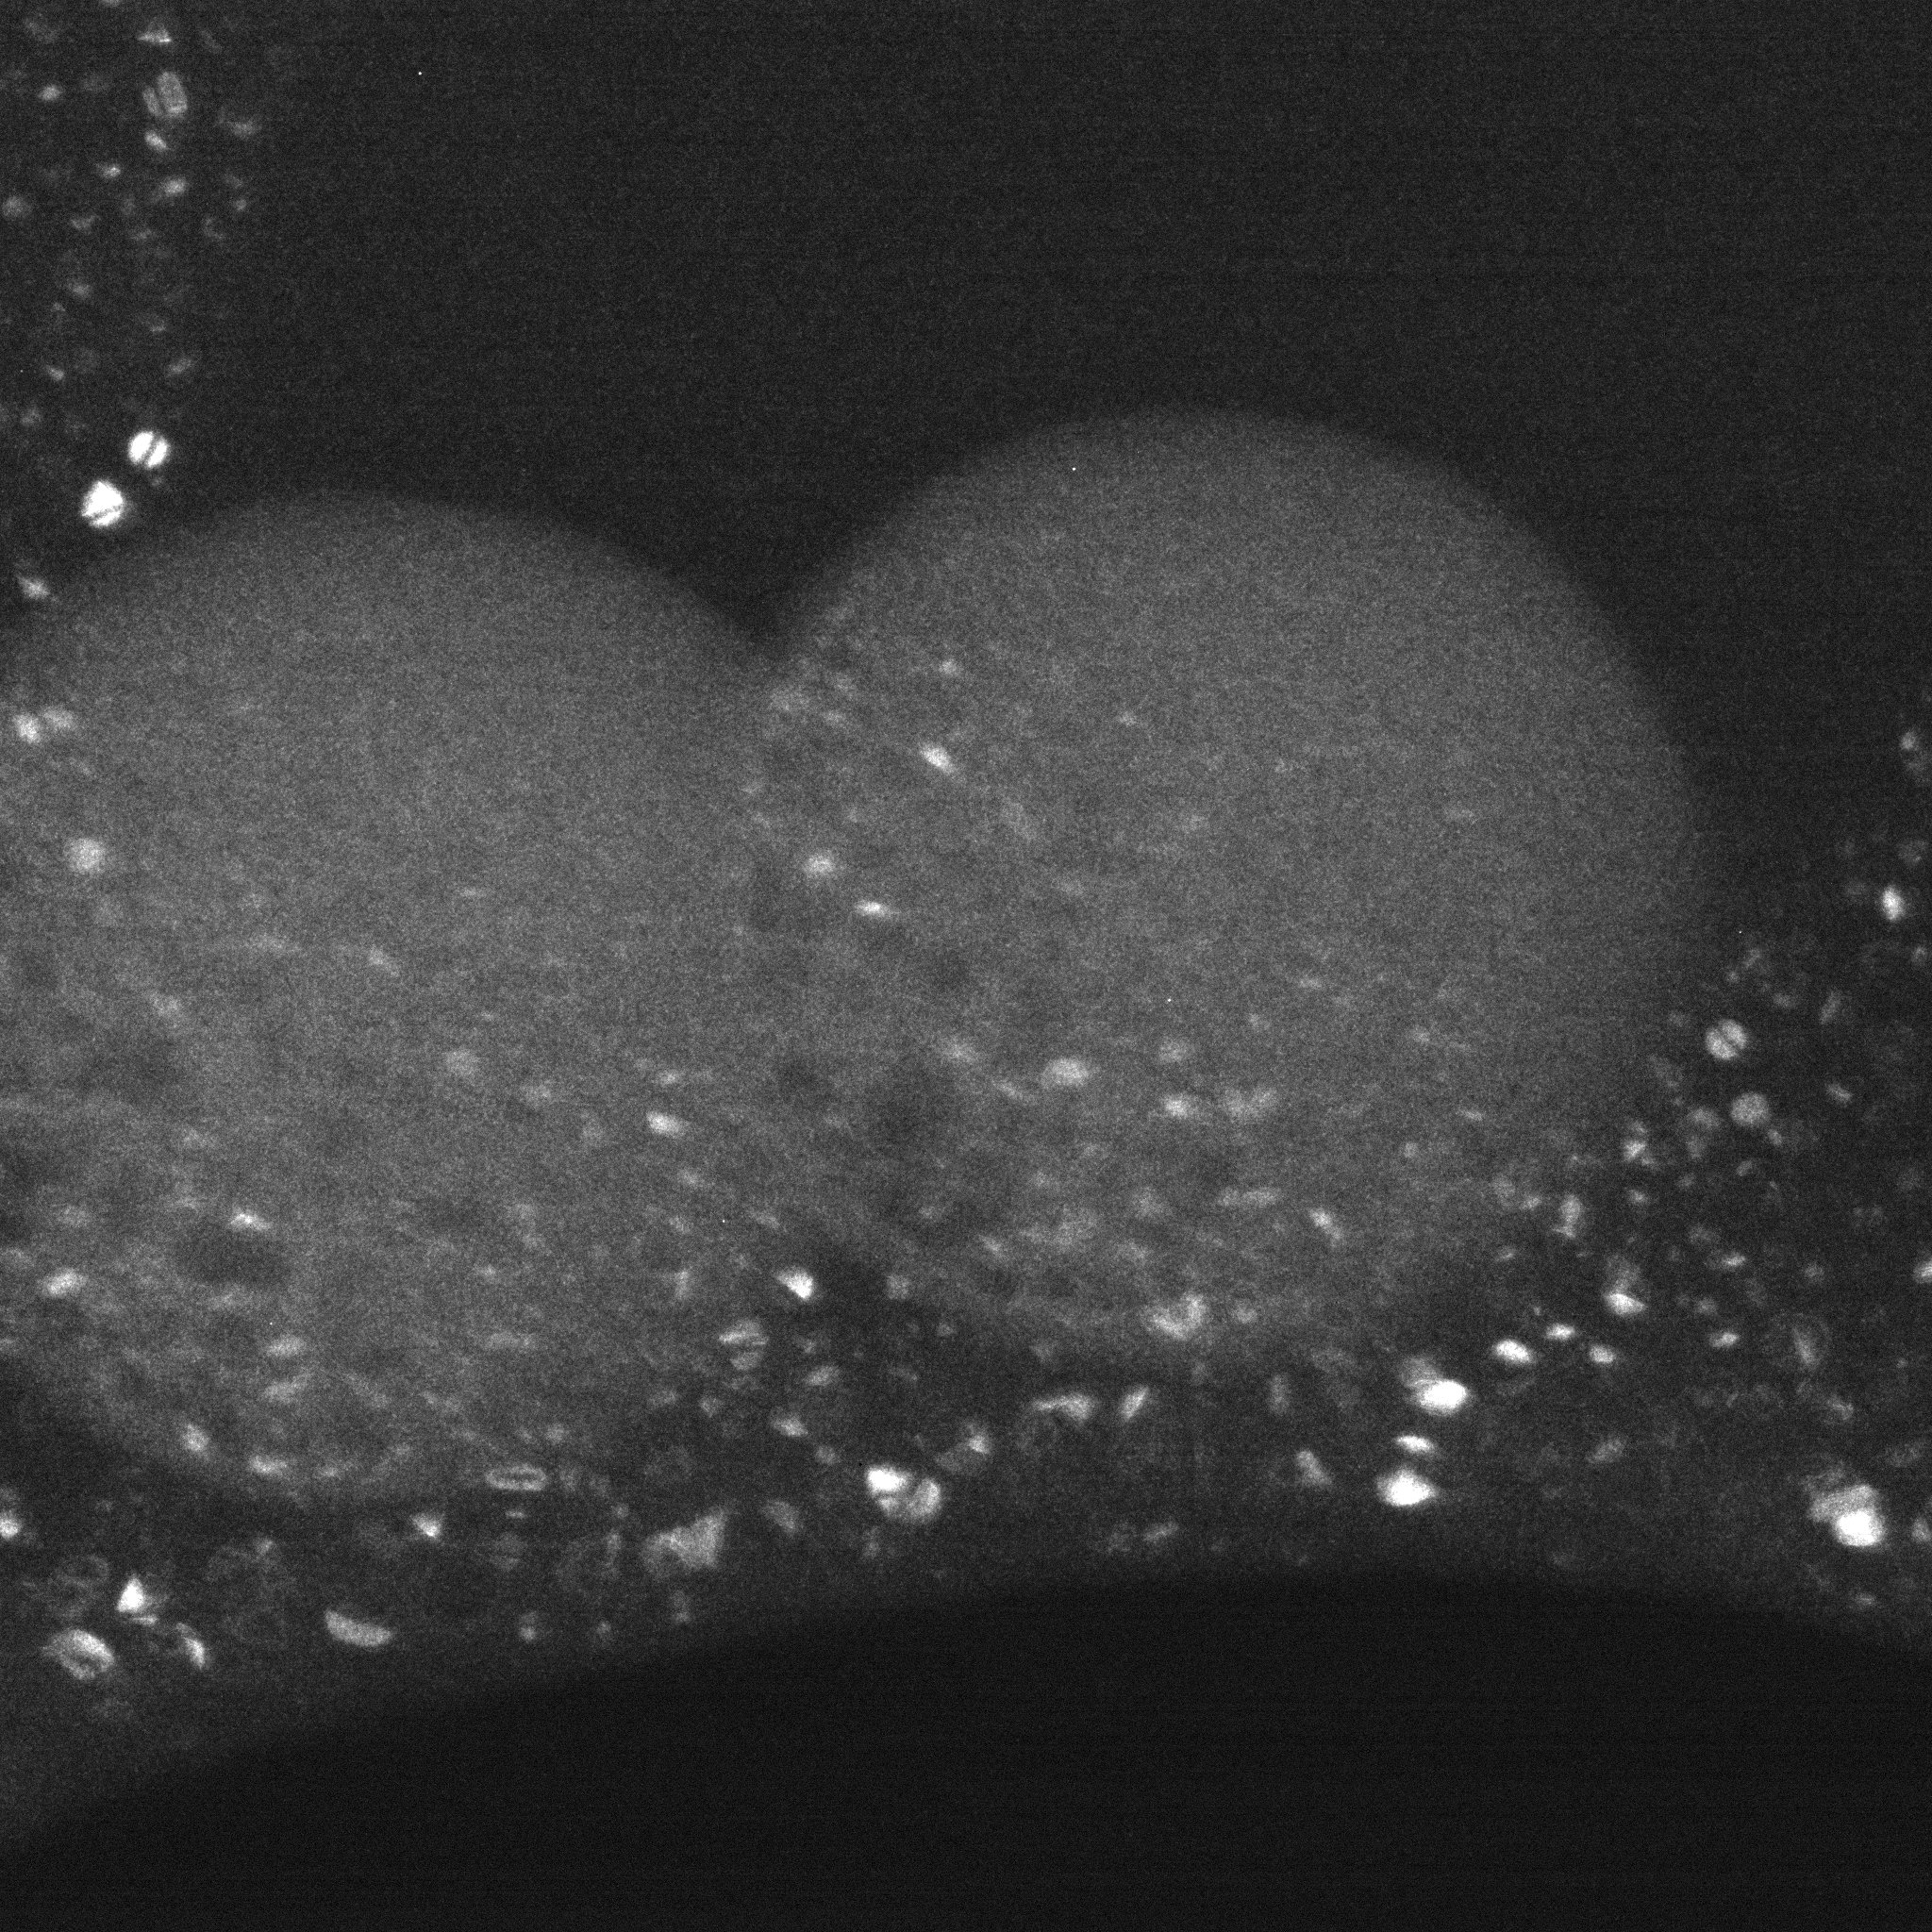
\includegraphics[width=\textwidth]{Grundlagen&Beugung/Goldpratikel_1sec_darkfeeld2_andererWinkel.jpg}
         \caption{Darkfield}
         \label{SPDF}
     \end{subfigure}
        \caption{Bright-/Centered Darkfield Aufnahme der Standard Probe (Kohlenstoff, Latex, Gold), 1 sec Beleuchtungszeit}
        \label{SPBF&DF}
\end{figure}

\subsection{InGaAs/GaAs Struktur}

Um die eigen angefertigt Probe aus der vorher beschriebenen Sektion „Probenpräperation“ genau zu untersuchen, mussten die Proben im Mikroskope getauscht werden. Dabei musste die das Schleusen und die Vakuum System wie zuvor aufgeführt bedient und gecheckt werden. Nach dem tauschen der Probe und einer Entlüftung und Stabilisierungszeit von ca. Einer Stunde musste das Mikroskope wieder neu eingereicht werden.  Dies wurde nach dem zuvor beschriebenen Schema durchgeführt.\\
An der eigenen Probe wurde zunächst versucht ein HRTEM Bild aufnehmen, Hierfür wurde ein geeignete dünne stelle an der Probe Identifiziert. Diese befand sich nahe der Klebesstelle an der Lochkante welches durch die Ionen Dünnung endstanden ist.\\
Nach dem Wechseln zum „Diffraction Mode“ konnte mithilfe der Beugungsbildes und den Kikuchi Linien die Probe so verkippt werden das TEM Aufnahmen entlang einer Zonenachse möglich war. Im Bild Modus wurde dann eine gute Aufnahme des Kristall Struktur mit atomarer Auflösung gemacht. Zudem wurden wieder Aufnahmen im unter-/Über Fokus erstellt. (Siehe Abbildung \cref{EigeneProbe}).

\begin{figure}
     \centering
     \begin{subfigure}[b]{0.49\textwidth}
         \centering
         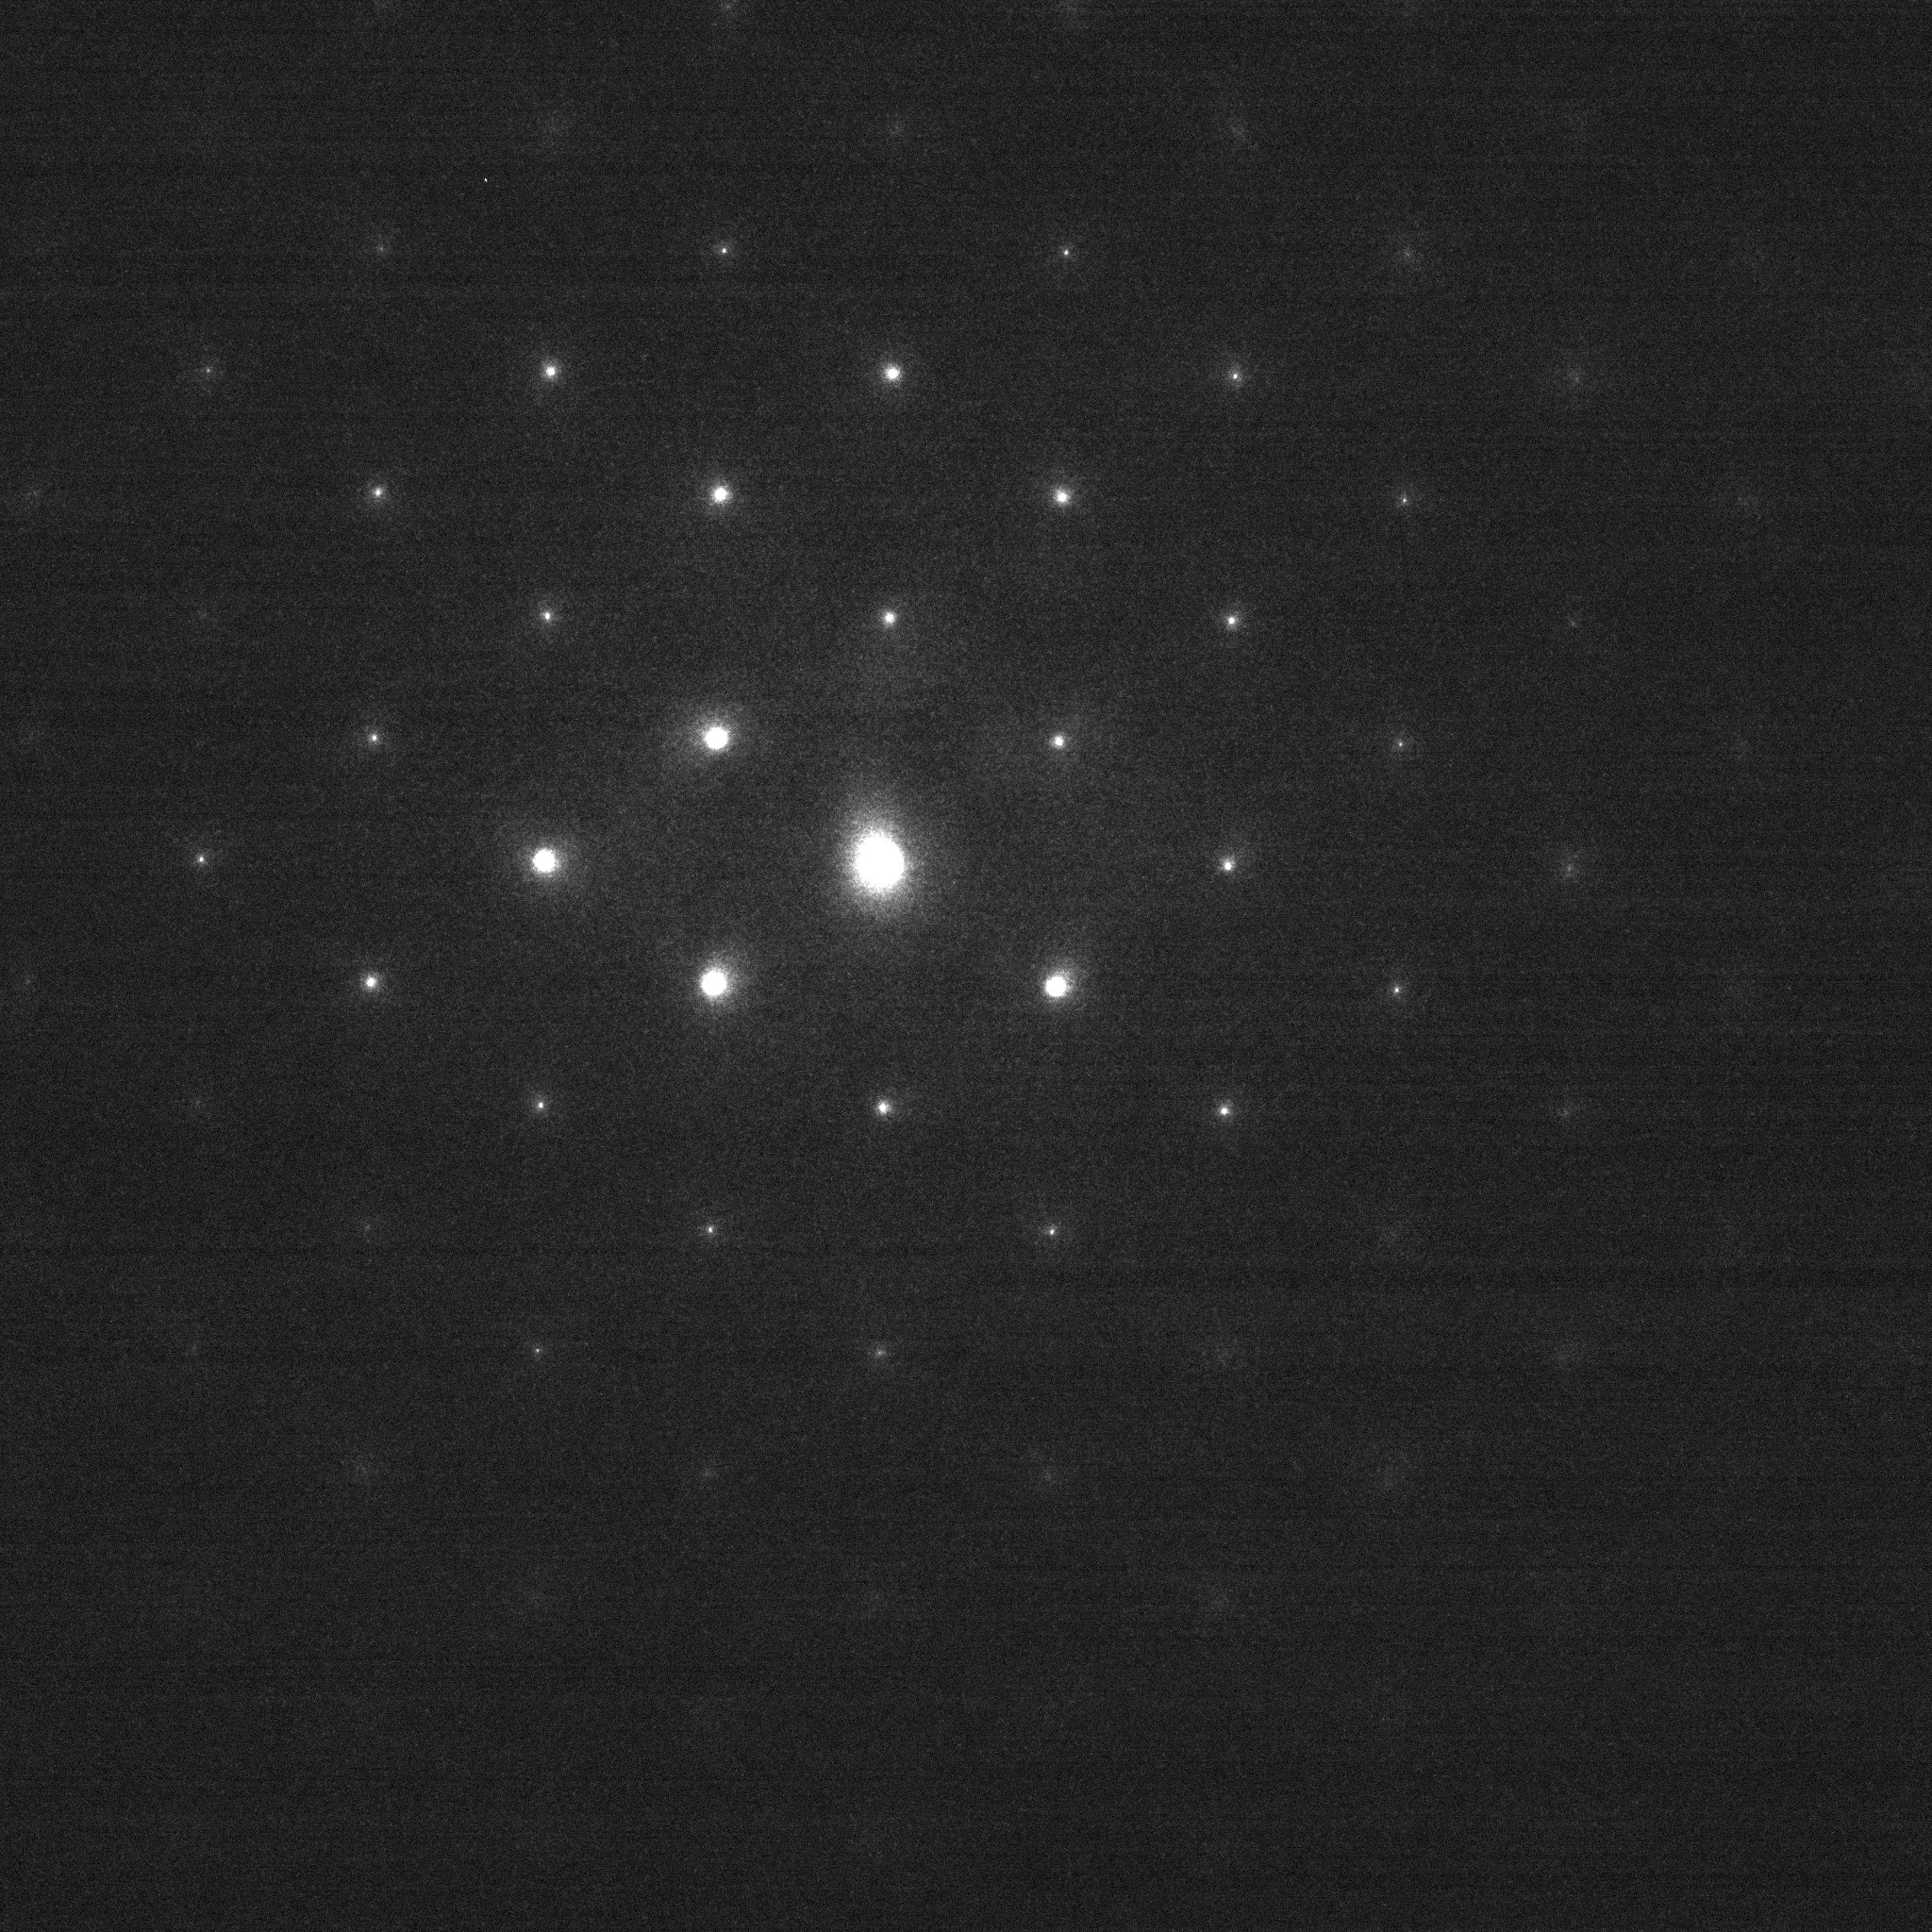
\includegraphics[width=\textwidth]{Grundlagen&Beugung/Eigenprobe_Beugungsbild_zonenachse1.jpg}
         \caption{Beugungsbild}
         \label{EPBB}
     \end{subfigure}
     \hfill
     \begin{subfigure}[b]{0.49\textwidth}
         \centering
         
\includegraphics[width=\textwidth]{Grundlagen&Beugung/Eigene_Probe_Schooeneaufnahme.jpg}
         \caption{Im Fokus}
         \label{EPFokus}
     \end{subfigure}
     \hfill
     \begin{subfigure}[b]{0.49\textwidth}
         \centering
         
\includegraphics[width=\textwidth]{Grundlagen&Beugung/Eigene_Probe_Unterfokus2.jpg}
         \caption{Unterfokus}
         \label{EPUnterfokus}
     \end{subfigure}
     \hfill
     \begin{subfigure}[b]{0.49\textwidth}
         \centering
         
\includegraphics[width=\textwidth]{Grundlagen&Beugung/Eigene_Porbe_Ueberfokus.jpg}
         \caption{Überfokus}
         \label{SPÜberfokus}
     \end{subfigure}
        \caption{HRTEM Aufnahmen der selbst angefertigten Probe. Mir Beugungsbild, Unterfokus und Überfokus. Beugungsbild Aufnahme entlang der Zonenachse (110), Gemessene Reflex Abstände zum nullstrahl: \(R1(200) = 7,148, R2(220) = 9.810 und R3(111) = 6.450\).}
        \label{EigeneProbe}
\end{figure}

Mit dem Beugungsbild wurde zunächst versucht die Zonenachse zu identifizieren, hierfür wurden mit Hilfe der Software „ImangeJ“ die Distanzen vom Nullstrahl zu den anliegenden Reflexen der XYZ Richtungen gemessen. \\
%R1=7,148/2 (3,574), Y = 9.810/2 (4,905), Z = 6,450/2 (3,225)
Mit Hilfe des Struktur Faktor Formel und dem Wissen das sie Probe ein GaAs Kristall ist, welcher eine FCC (Face Centered Cubic) ist kann folgende Relation gefunden werden.
\[
    \frac{R_i}{R_j} = \frac{\sqrt{h_i^2+k_i^2+l_i^2}}{\sqrt{h_j^2+k_j^2+l_j^2}}
.\]
Dabei können nur Reflexe entstehen wenn hkl alle grade oder ungerade Werte haben, bei gemischten indeces ist der Strukturfaktor 0.
\[
    z.B. = 000, 111, 200, 220, 311, 222, 400, 331, 420, …
.\]
Mit einsetzen der gemessenen Längen und einsetzen verschiedener möglicher hkl Werte, wurden folgende Reflexe identifiziert.
\[
R_1 = (002), R_2 = (220), R_3 = (111) 
.\]
Die Zonenachse muss dementsprechend orthogonal zu diesen drei Achsen sein welche auf die [110] zutrifft.\\
Um auch aufnahmen an entlang anderen Zonenachsen zu erstellen wurde die Probe entlang der [001] Achse verkippt bis wieder ein zentriertes Beugungsbild erkennbar war. (siehe Abbildung \cref{EP2BB}).\\
Hierbei wurden die (020), (200) und (220) Reflexe beobachtet, so dass die Zonenachse nun bei [001] war.

\begin{figure}[htbp]
 \centering
 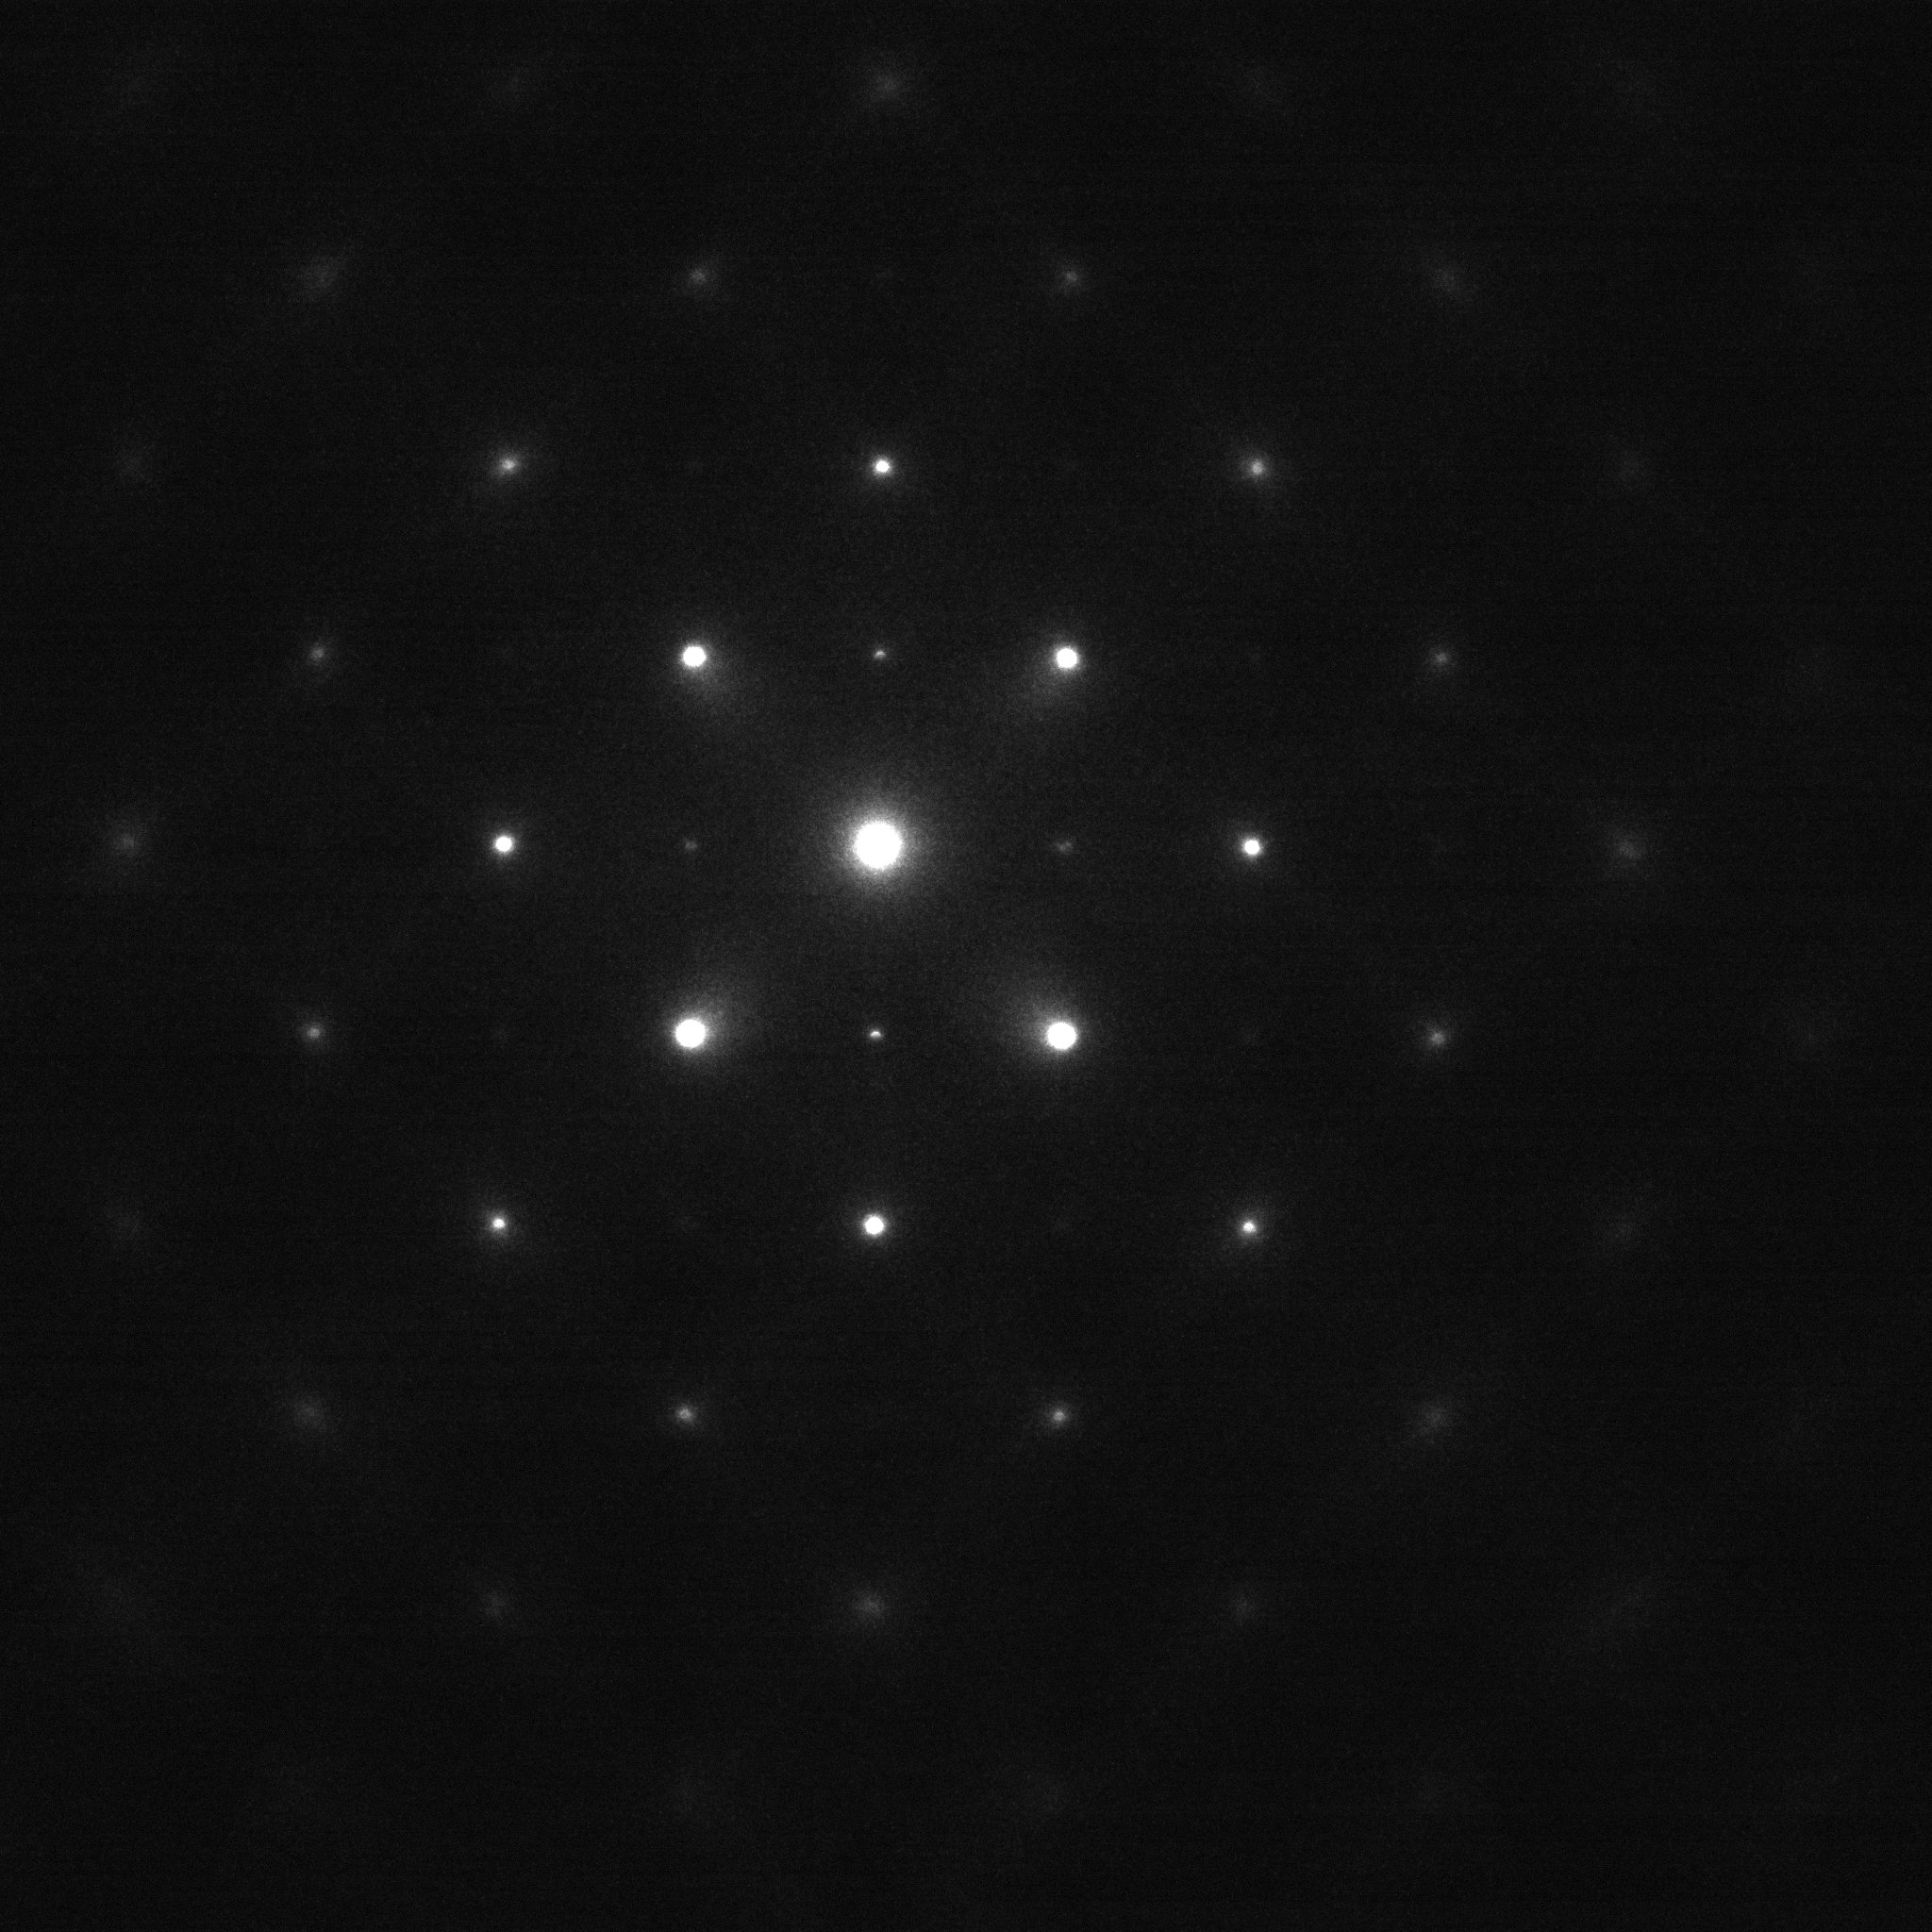
\includegraphics[width=0.7\textwidth]{Grundlagen&Beugung/Eigene_probe_Andere_seite_difraction.jpg}
 \caption[Beugungsbild(001)]{Beugungsbild Aufnahme entlang der Zonenachse (001), Gemessene Reflex Abstände zum nullstrahl: \( R_1(020)=7,086, R_2(220)= 6,98 und R_3(200)= 4,824 \).}
 \label{EP2BB}
\end{figure}

\subsubsection{CBED Aufnahmen}
CBED steht für „Convergent Beam Electron Diffraction“ dies bedeutet das wir im Beugung Modus einen Beleuchtungsstrahl haben der nicht mehr wie zuvor parallel, sondern Konvergent die Probe beleuchtet. Dabei weiten sich auch die Beugungsreflexe zu scheiben auf. Bei weiterer Aufweitung können die beugungsscheiben überschneiden und miteinander interferieren, dadurch werden die Kikuchi Lienen besonderes sichtbar.  Mit Hilfe von CEBD können mehrfachstreuengen der HOLZ Linien an dicken Proben abgebildet werden. Die Symmetrie des Kristals kann untersucht werden. Durch die Symmetrie der Beugungsbilder kann eine Chemische Sensitivität erreicht werden. An bestimmten Zonenachsen können Atome Positionen bestimmt werden.\\
Eine Reihe von CBED aufnahmen der GaAs Probe ist unten aufgeführt, dabei wurde die Beleuchtung von parallel zu konvergent angepasst.

\begin{figure}
     \centering
     \begin{subfigure}[b]{0.3\textwidth}
         \centering
         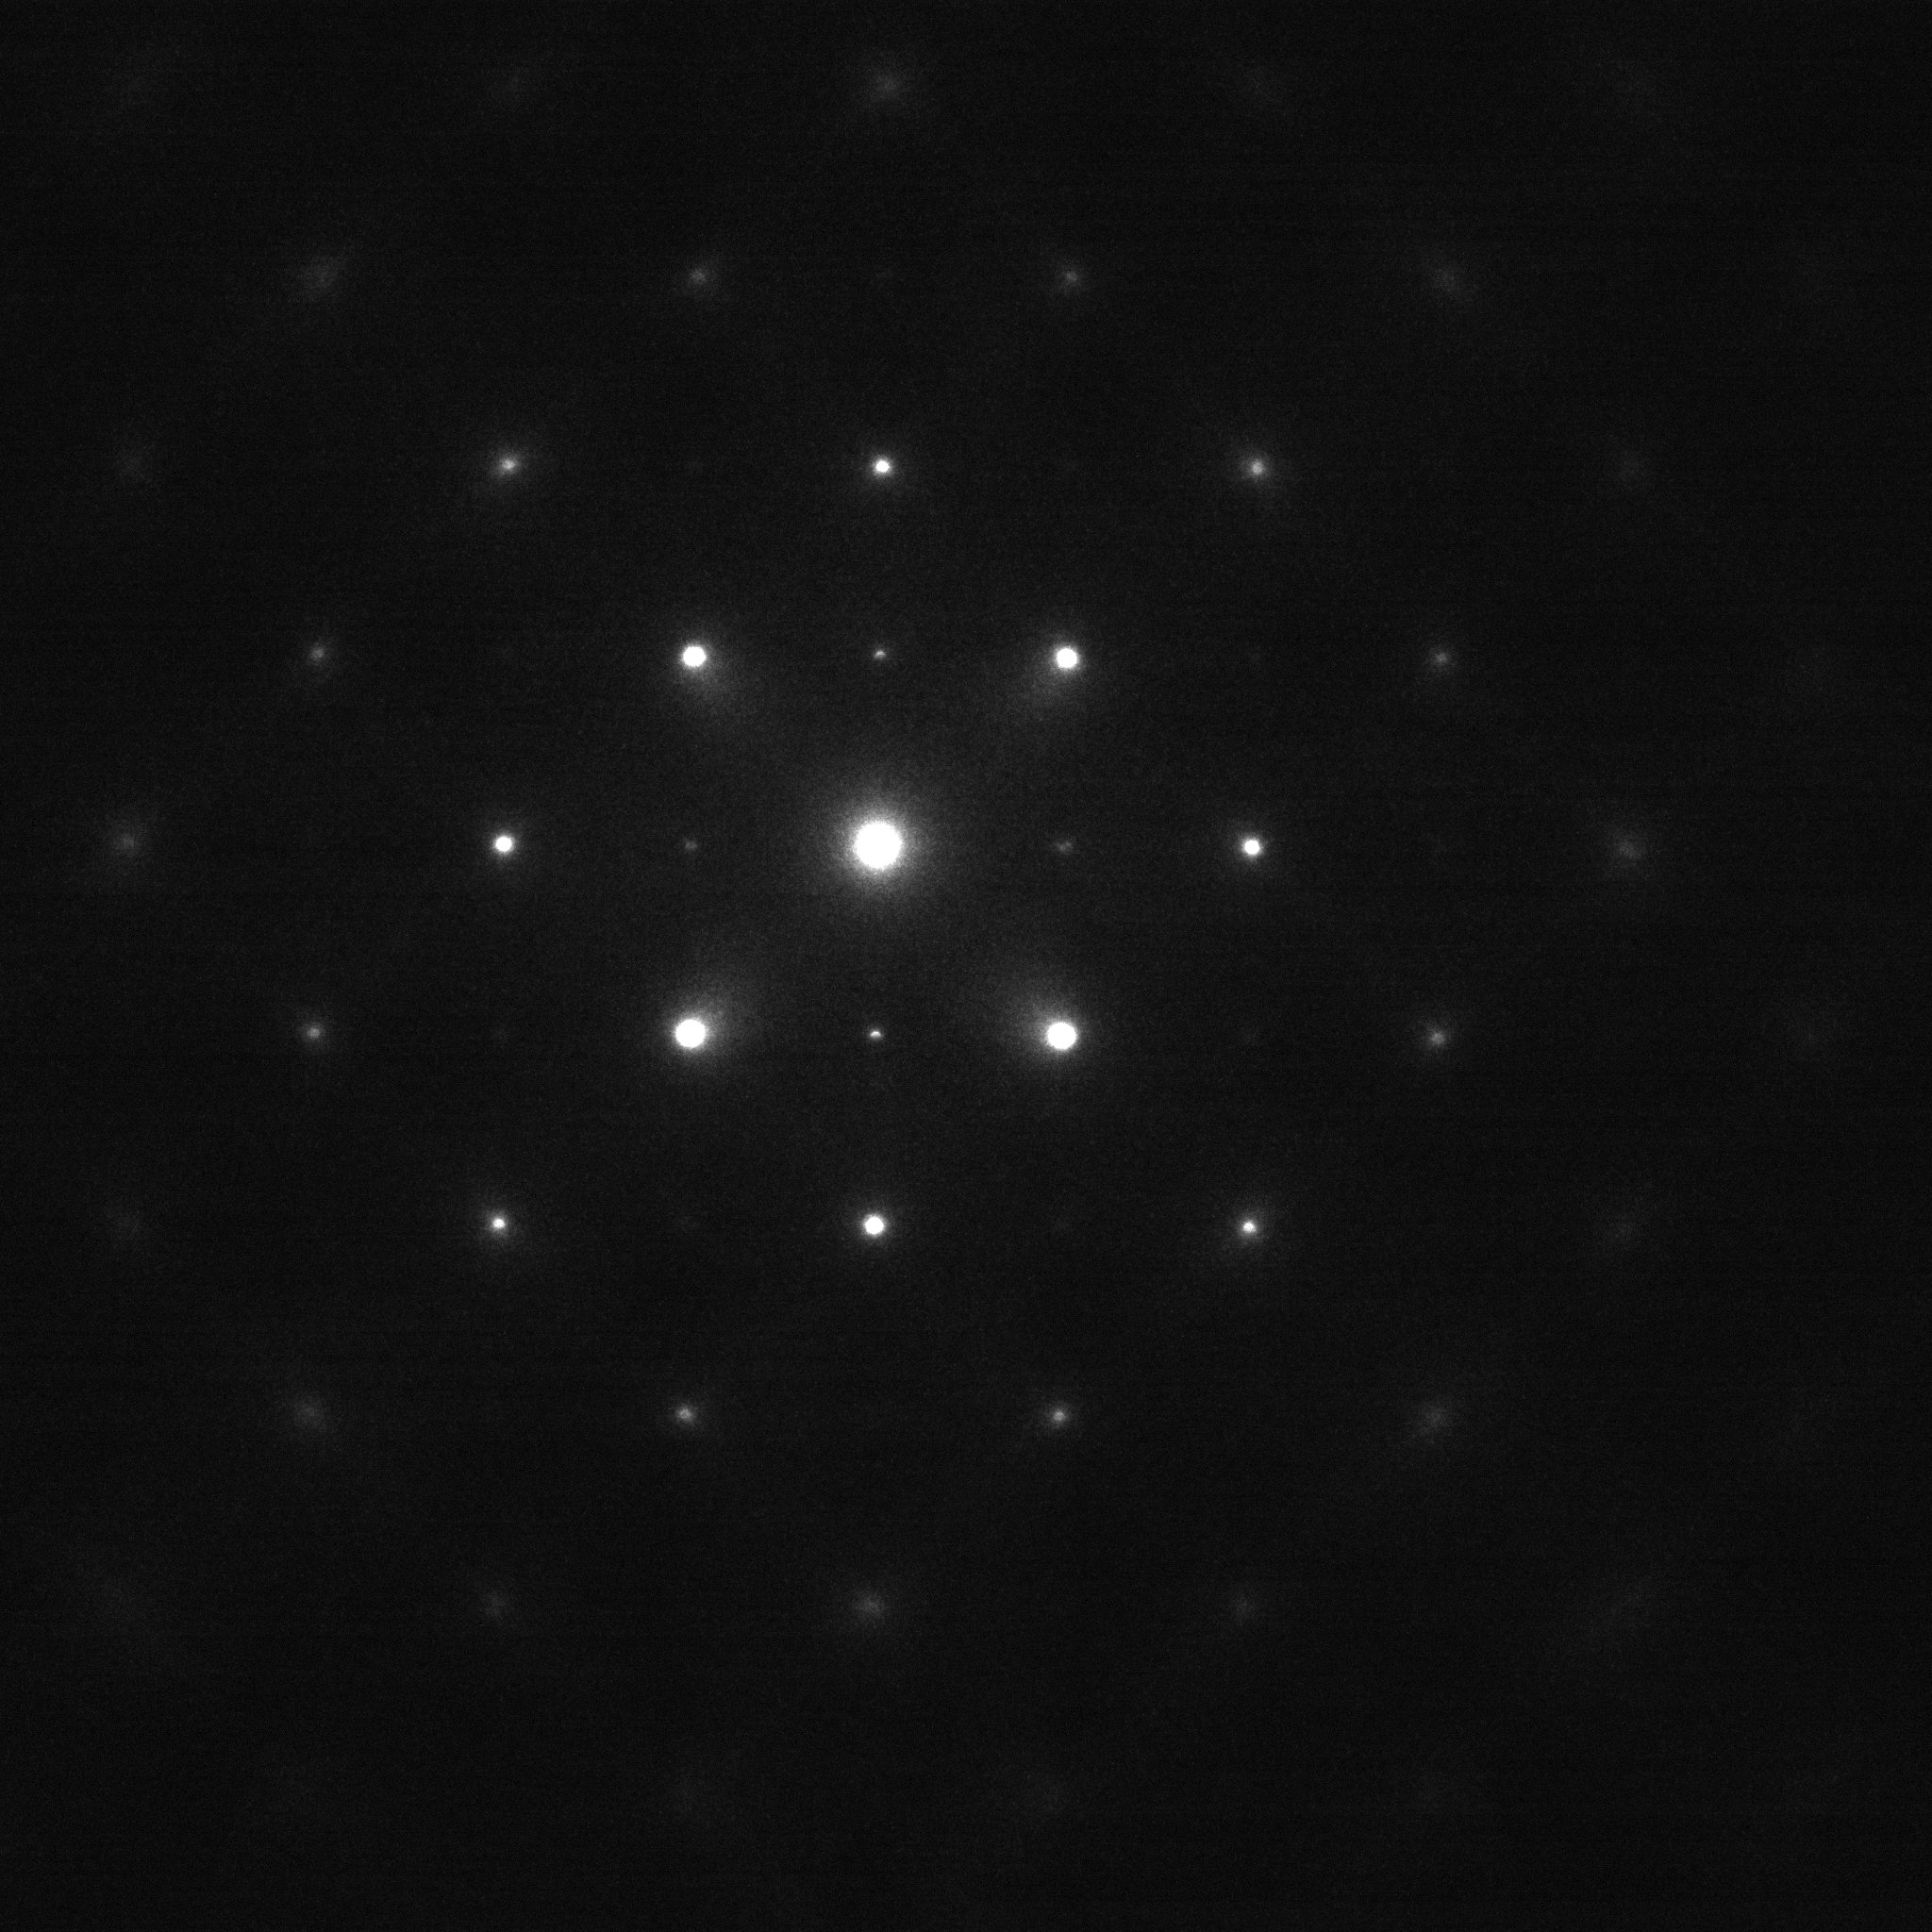
\includegraphics[width=\textwidth]{Grundlagen&Beugung/CBED1.jpg}
         \caption{Parallel}
         \label{CBEDP}
     \end{subfigure}
     \hfill
     \begin{subfigure}[b]{0.3\textwidth}
         \centering
         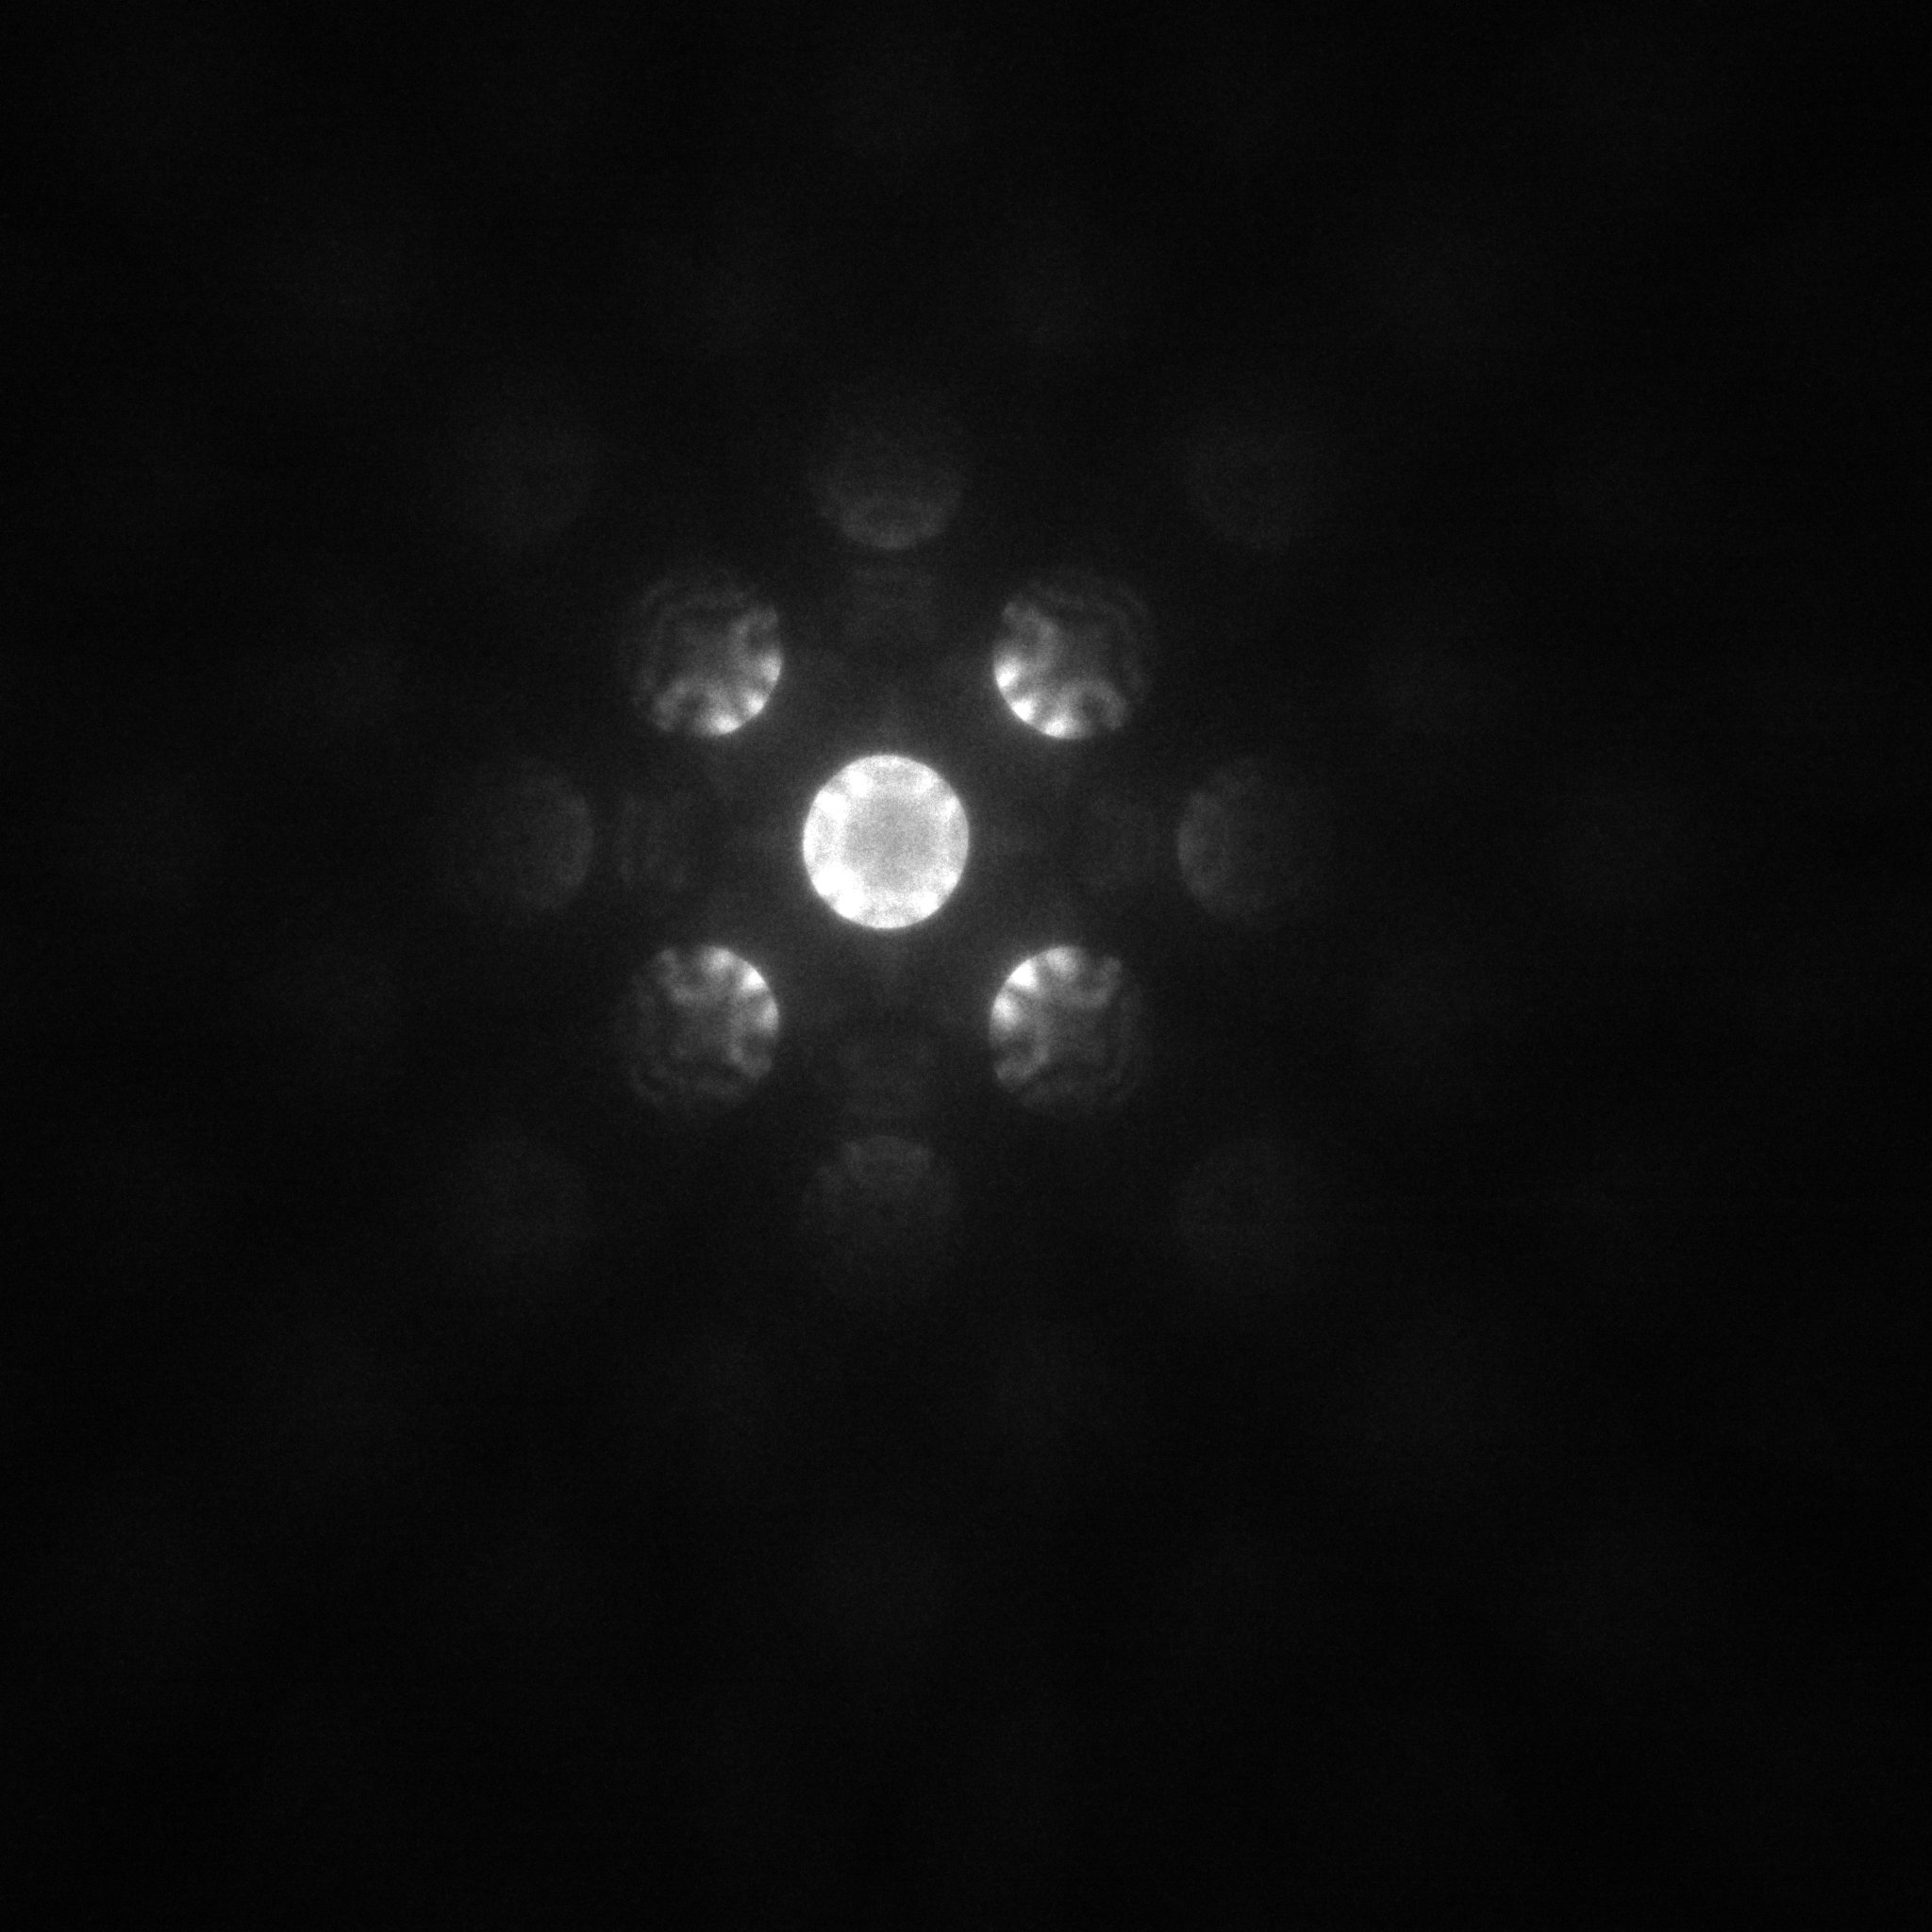
\includegraphics[width=\textwidth]{Grundlagen&Beugung/CBED2.jpg}
         \caption{semi-Konvergent}
         \label{CBEDSK}
     \end{subfigure}
     \hfill
     \begin{subfigure}[b]{0.3\textwidth}
         \centering
         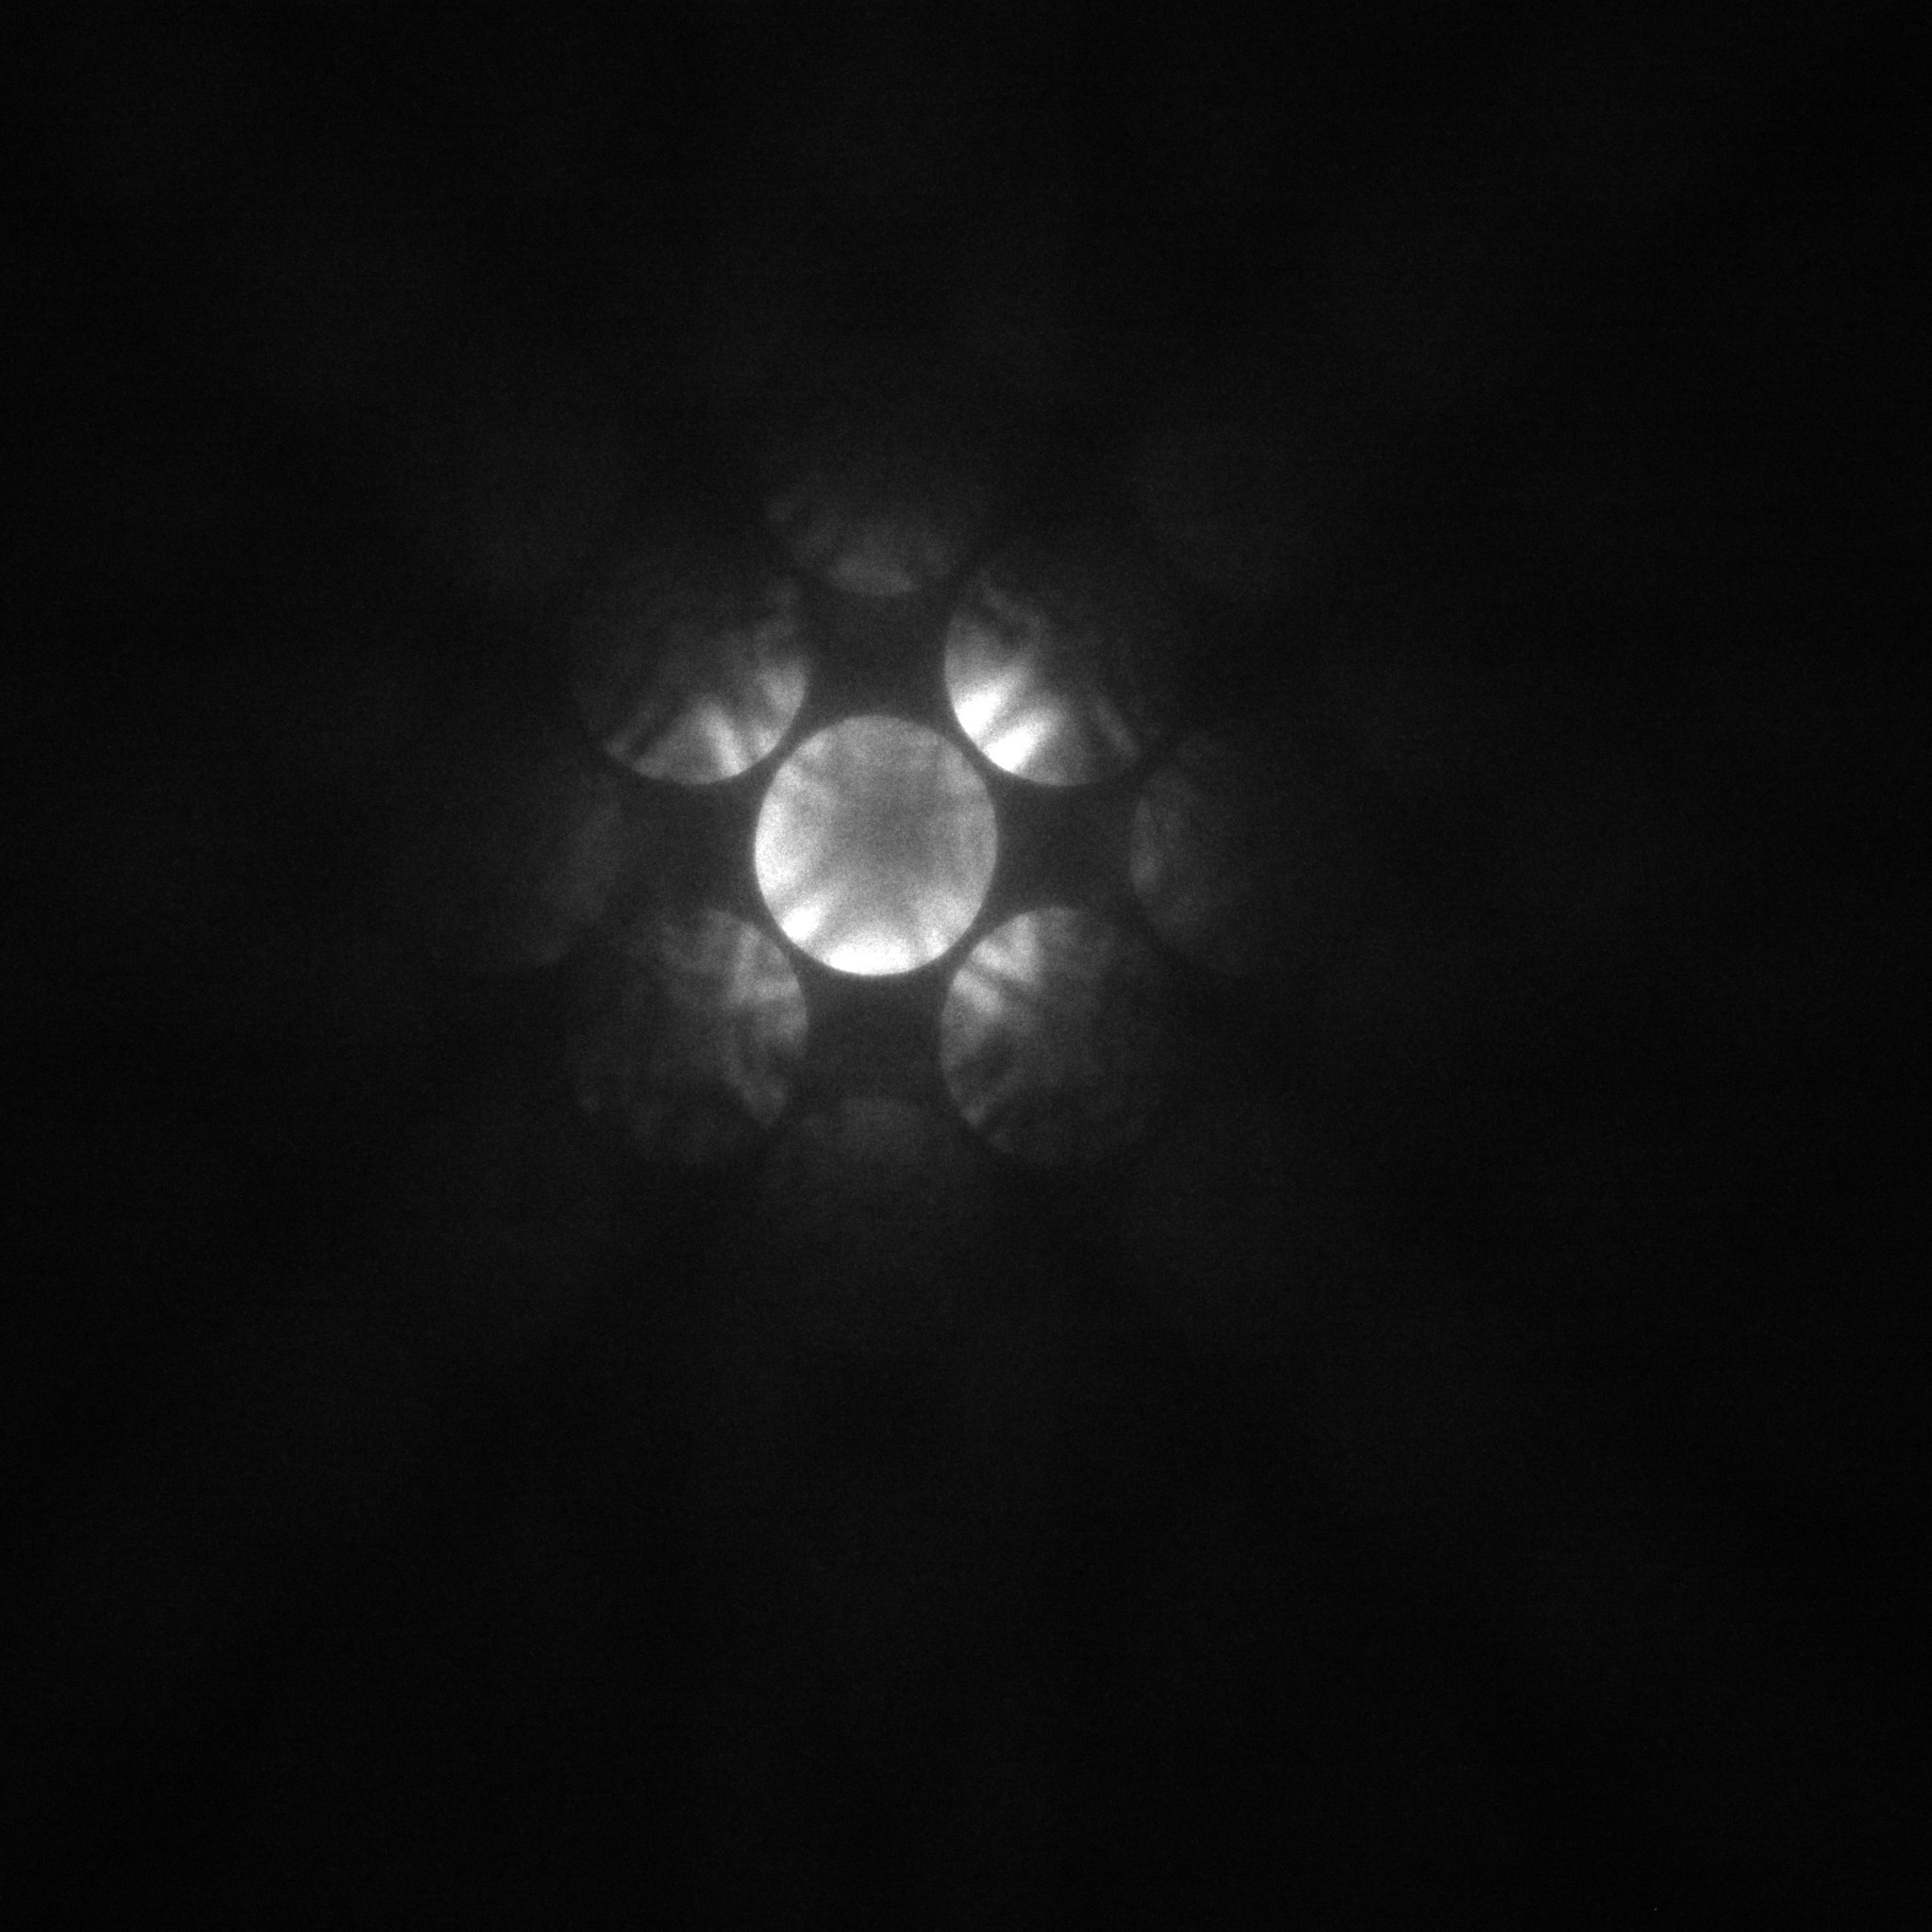
\includegraphics[width=\textwidth]{Grundlagen&Beugung/CBED3.jpg}
         \caption{Konvergent}
         \label{CBEDK}
     \end{subfigure}
        \caption{CBED Aufnehmen der Selbst erstellten GaAs Probe mit verschiedenen Konvergenten Winkeln \(\alpha\)}
        \label{CBED}
\end{figure}

Die GaAs Probe wurde sich im HRTEM im Bildmodus noch etwas angeschaut, dabei sind Zwei Interessante Segmente von besondere Interesse gewesen. 
Zunächst ein Aluminiumbelt (siehe \cref{EPBF&DFAl}). Das Al Belt ist gut in der Hellfeld Aufnahme zu erkennen, da sie einen sehr hohen Kontrast zum GaAs hat, es ist der Dunkler Steifen auf an der Oberseite des Bild. Zusätzlich sind in dieser Aufnahme die Quantum Belts, Untere Seite, zu erkennen und die Klebe stelle an der die beiden proben Segmente verklebt wurden. An der Klebe stelle sind außerdem „Bending Contures“ im GaAs an beiden Seiten erkennbar.

\begin{figure}
     \centering
     \begin{subfigure}[b]{0.49\textwidth}
         \centering
         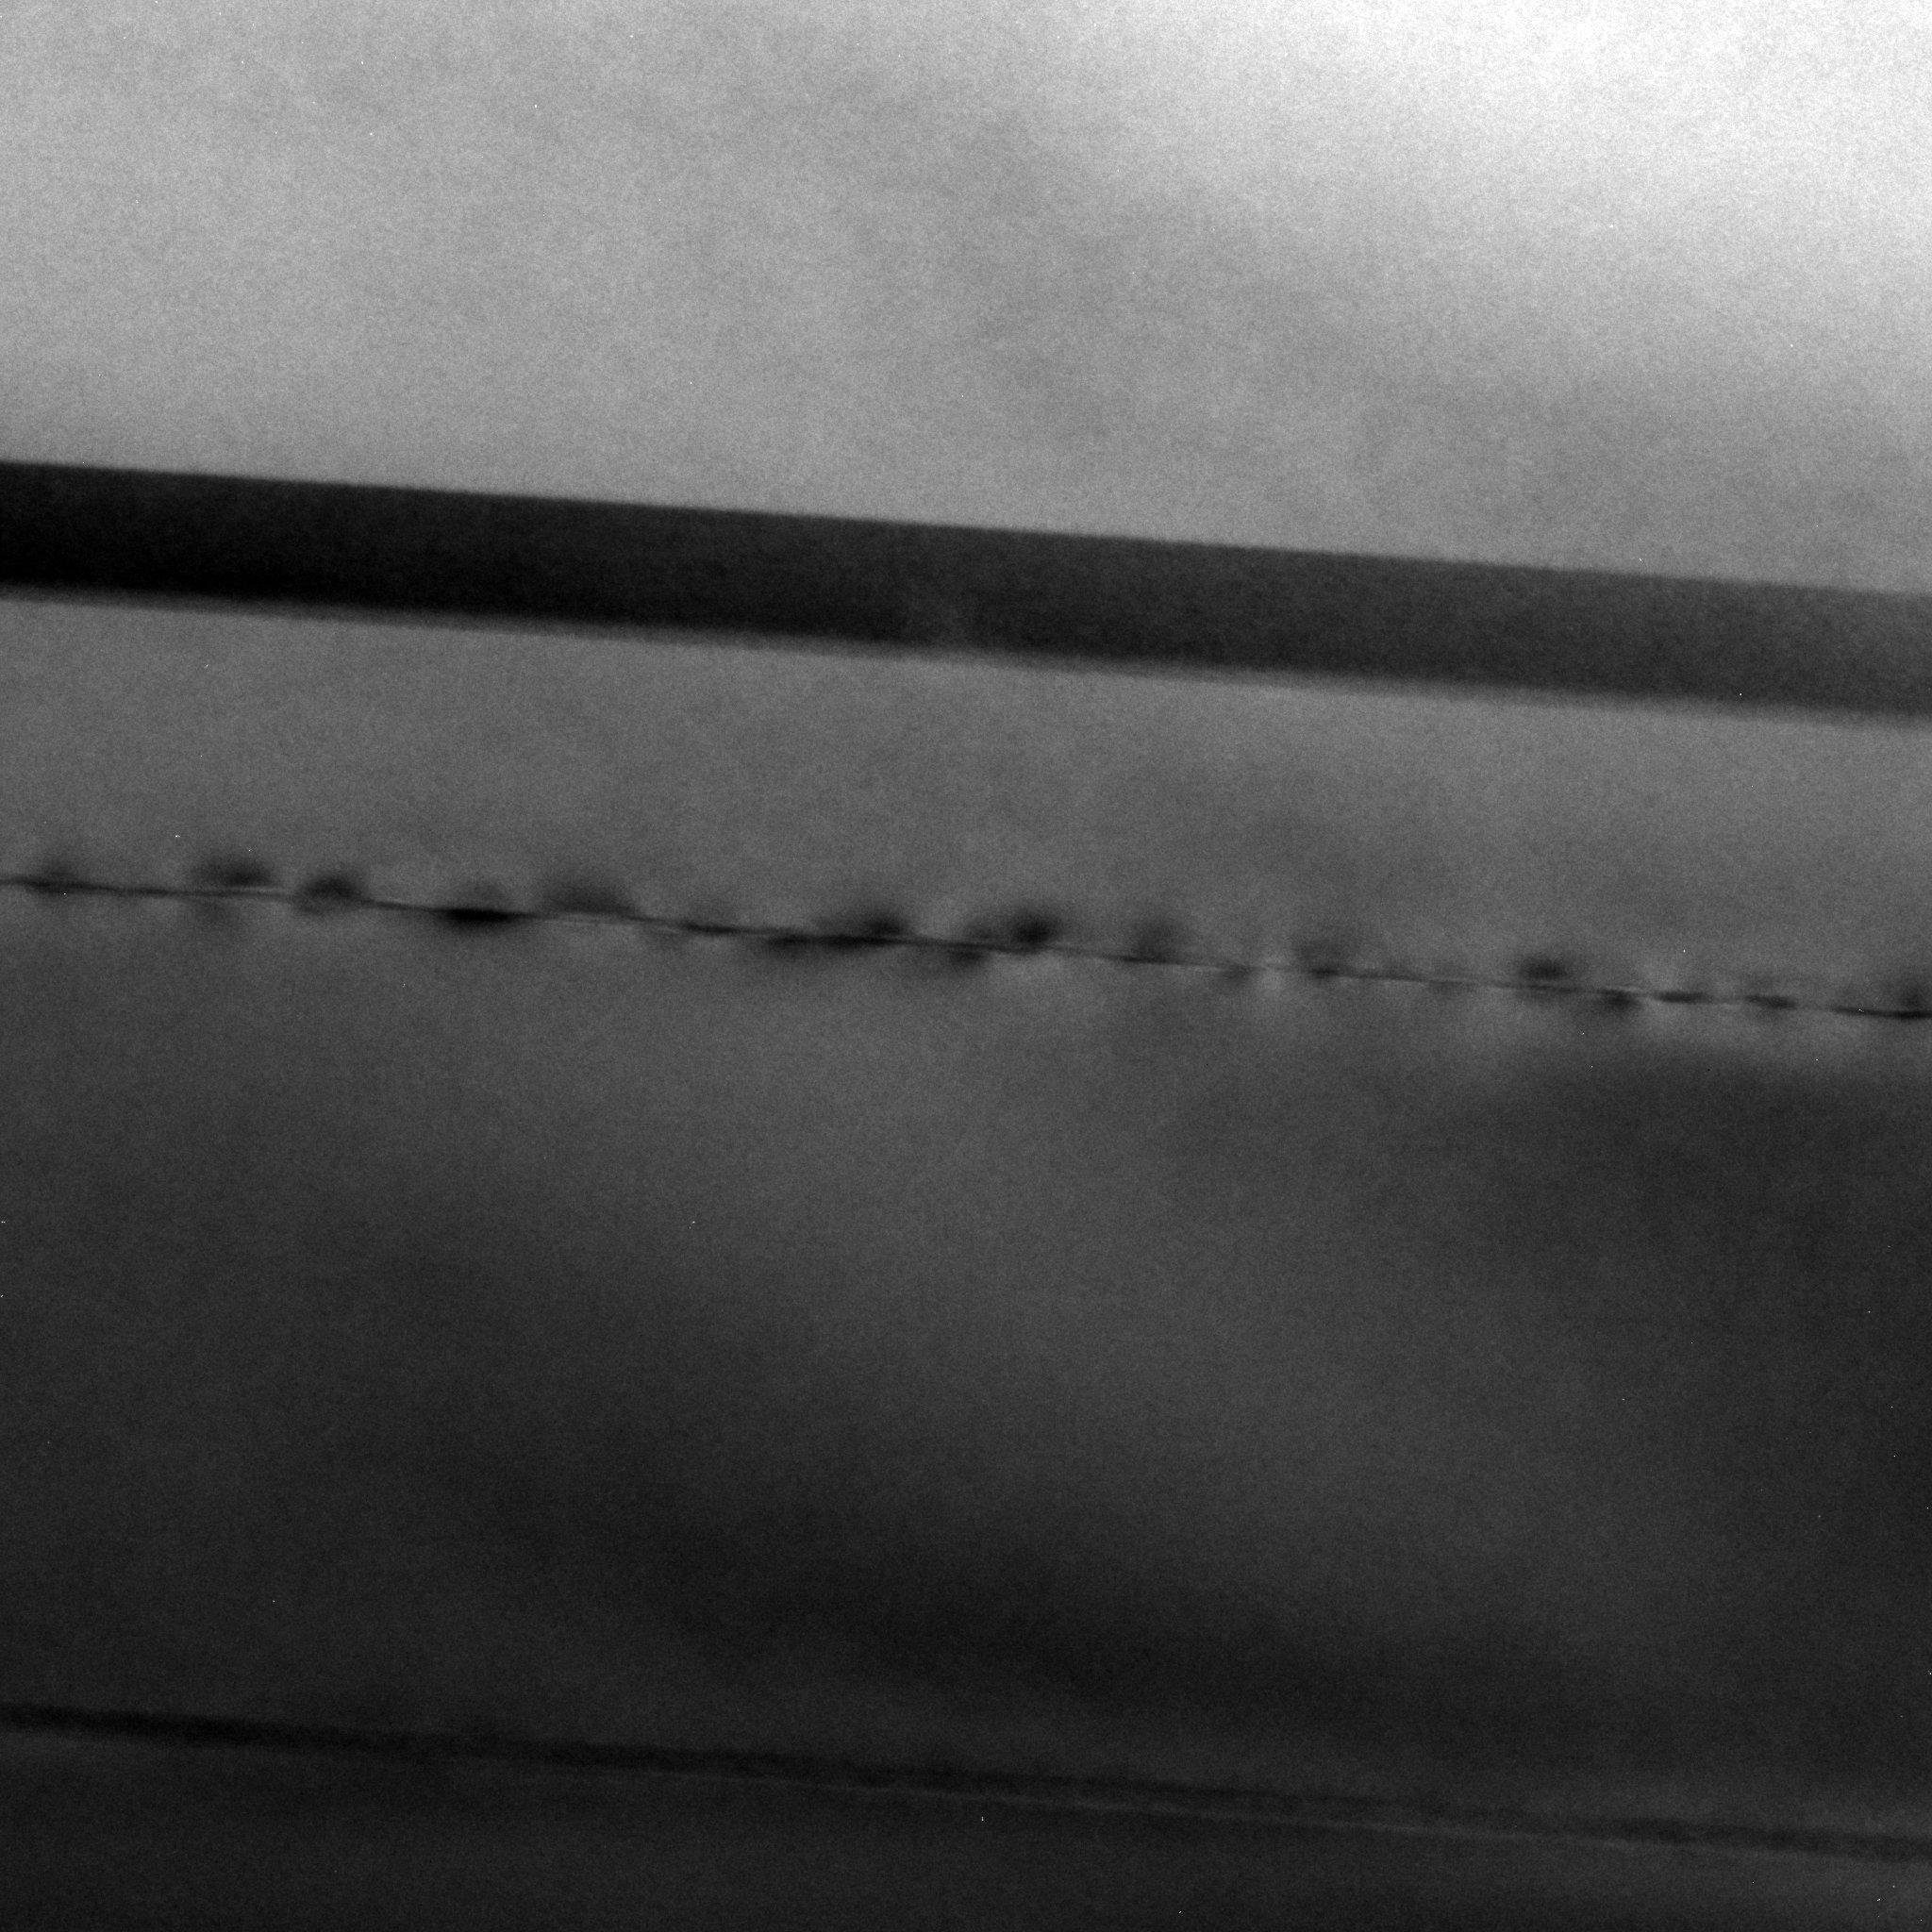
\includegraphics[width=\textwidth]{Grundlagen&Beugung/Eigeneprobe_BF_Al_Belt.jpg}
         \caption{Brightfield}
         \label{EPBFAl}
     \end{subfigure}
     \hfill
     \begin{subfigure}[b]{0.49\textwidth}
         \centering
         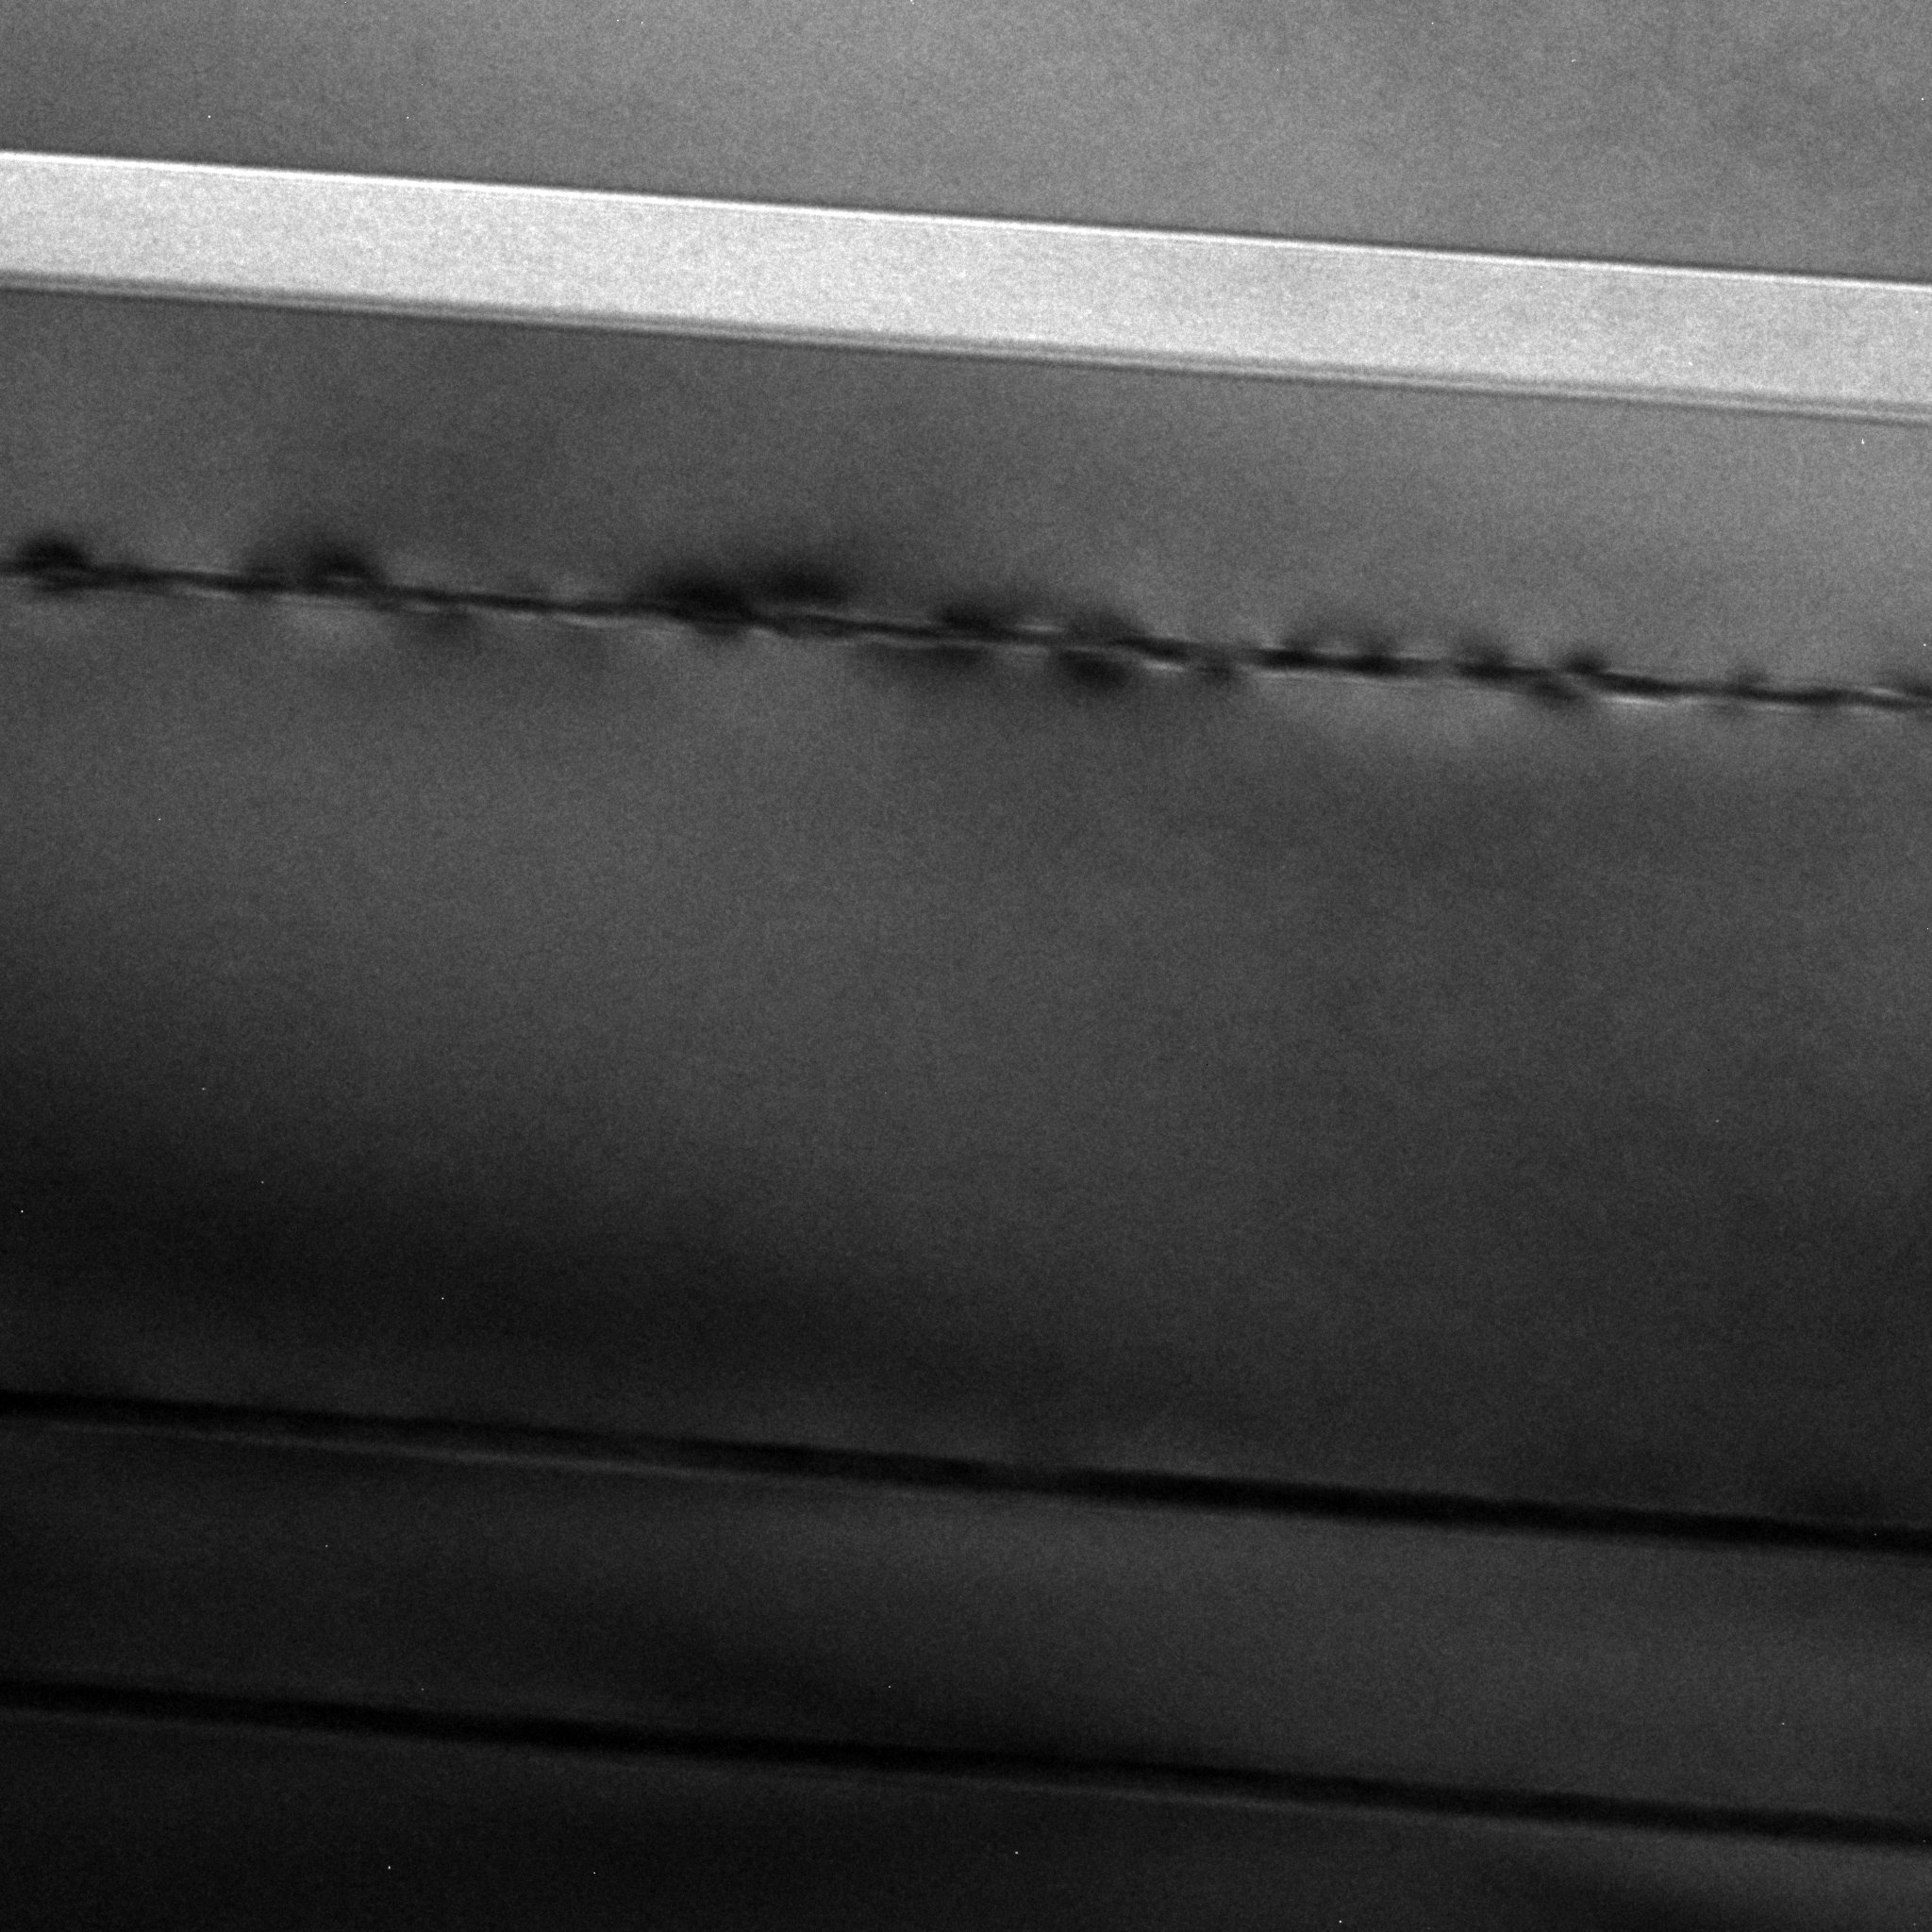
\includegraphics[width=\textwidth]{Grundlagen&Beugung/Eigeneprobe_DF_Al_Beld.jpg}
         \caption{Darkfield}
         \label{EPDFAl}
     \end{subfigure}
        \caption{TEM Darkfield und Brightfield Aufnahme GaAs Probe mit Al Belt.}
        \label{EPBF&DFAl}
\end{figure}

Die nächsten aufnahmen (Siehe \cref{EPBF&DFQB}) sind von den Quantum Belts, es wurden Jeweils Hell und Dunkel Feld aufnahmen. In der Dunkelfeld Aufnahme ist durch den hohen Kontrast die unterschiedliche dicke der Quantum Belts gut zu erkennen. 

\begin{figure}
     \centering
     \begin{subfigure}[b]{0.49\textwidth}
         \centering
         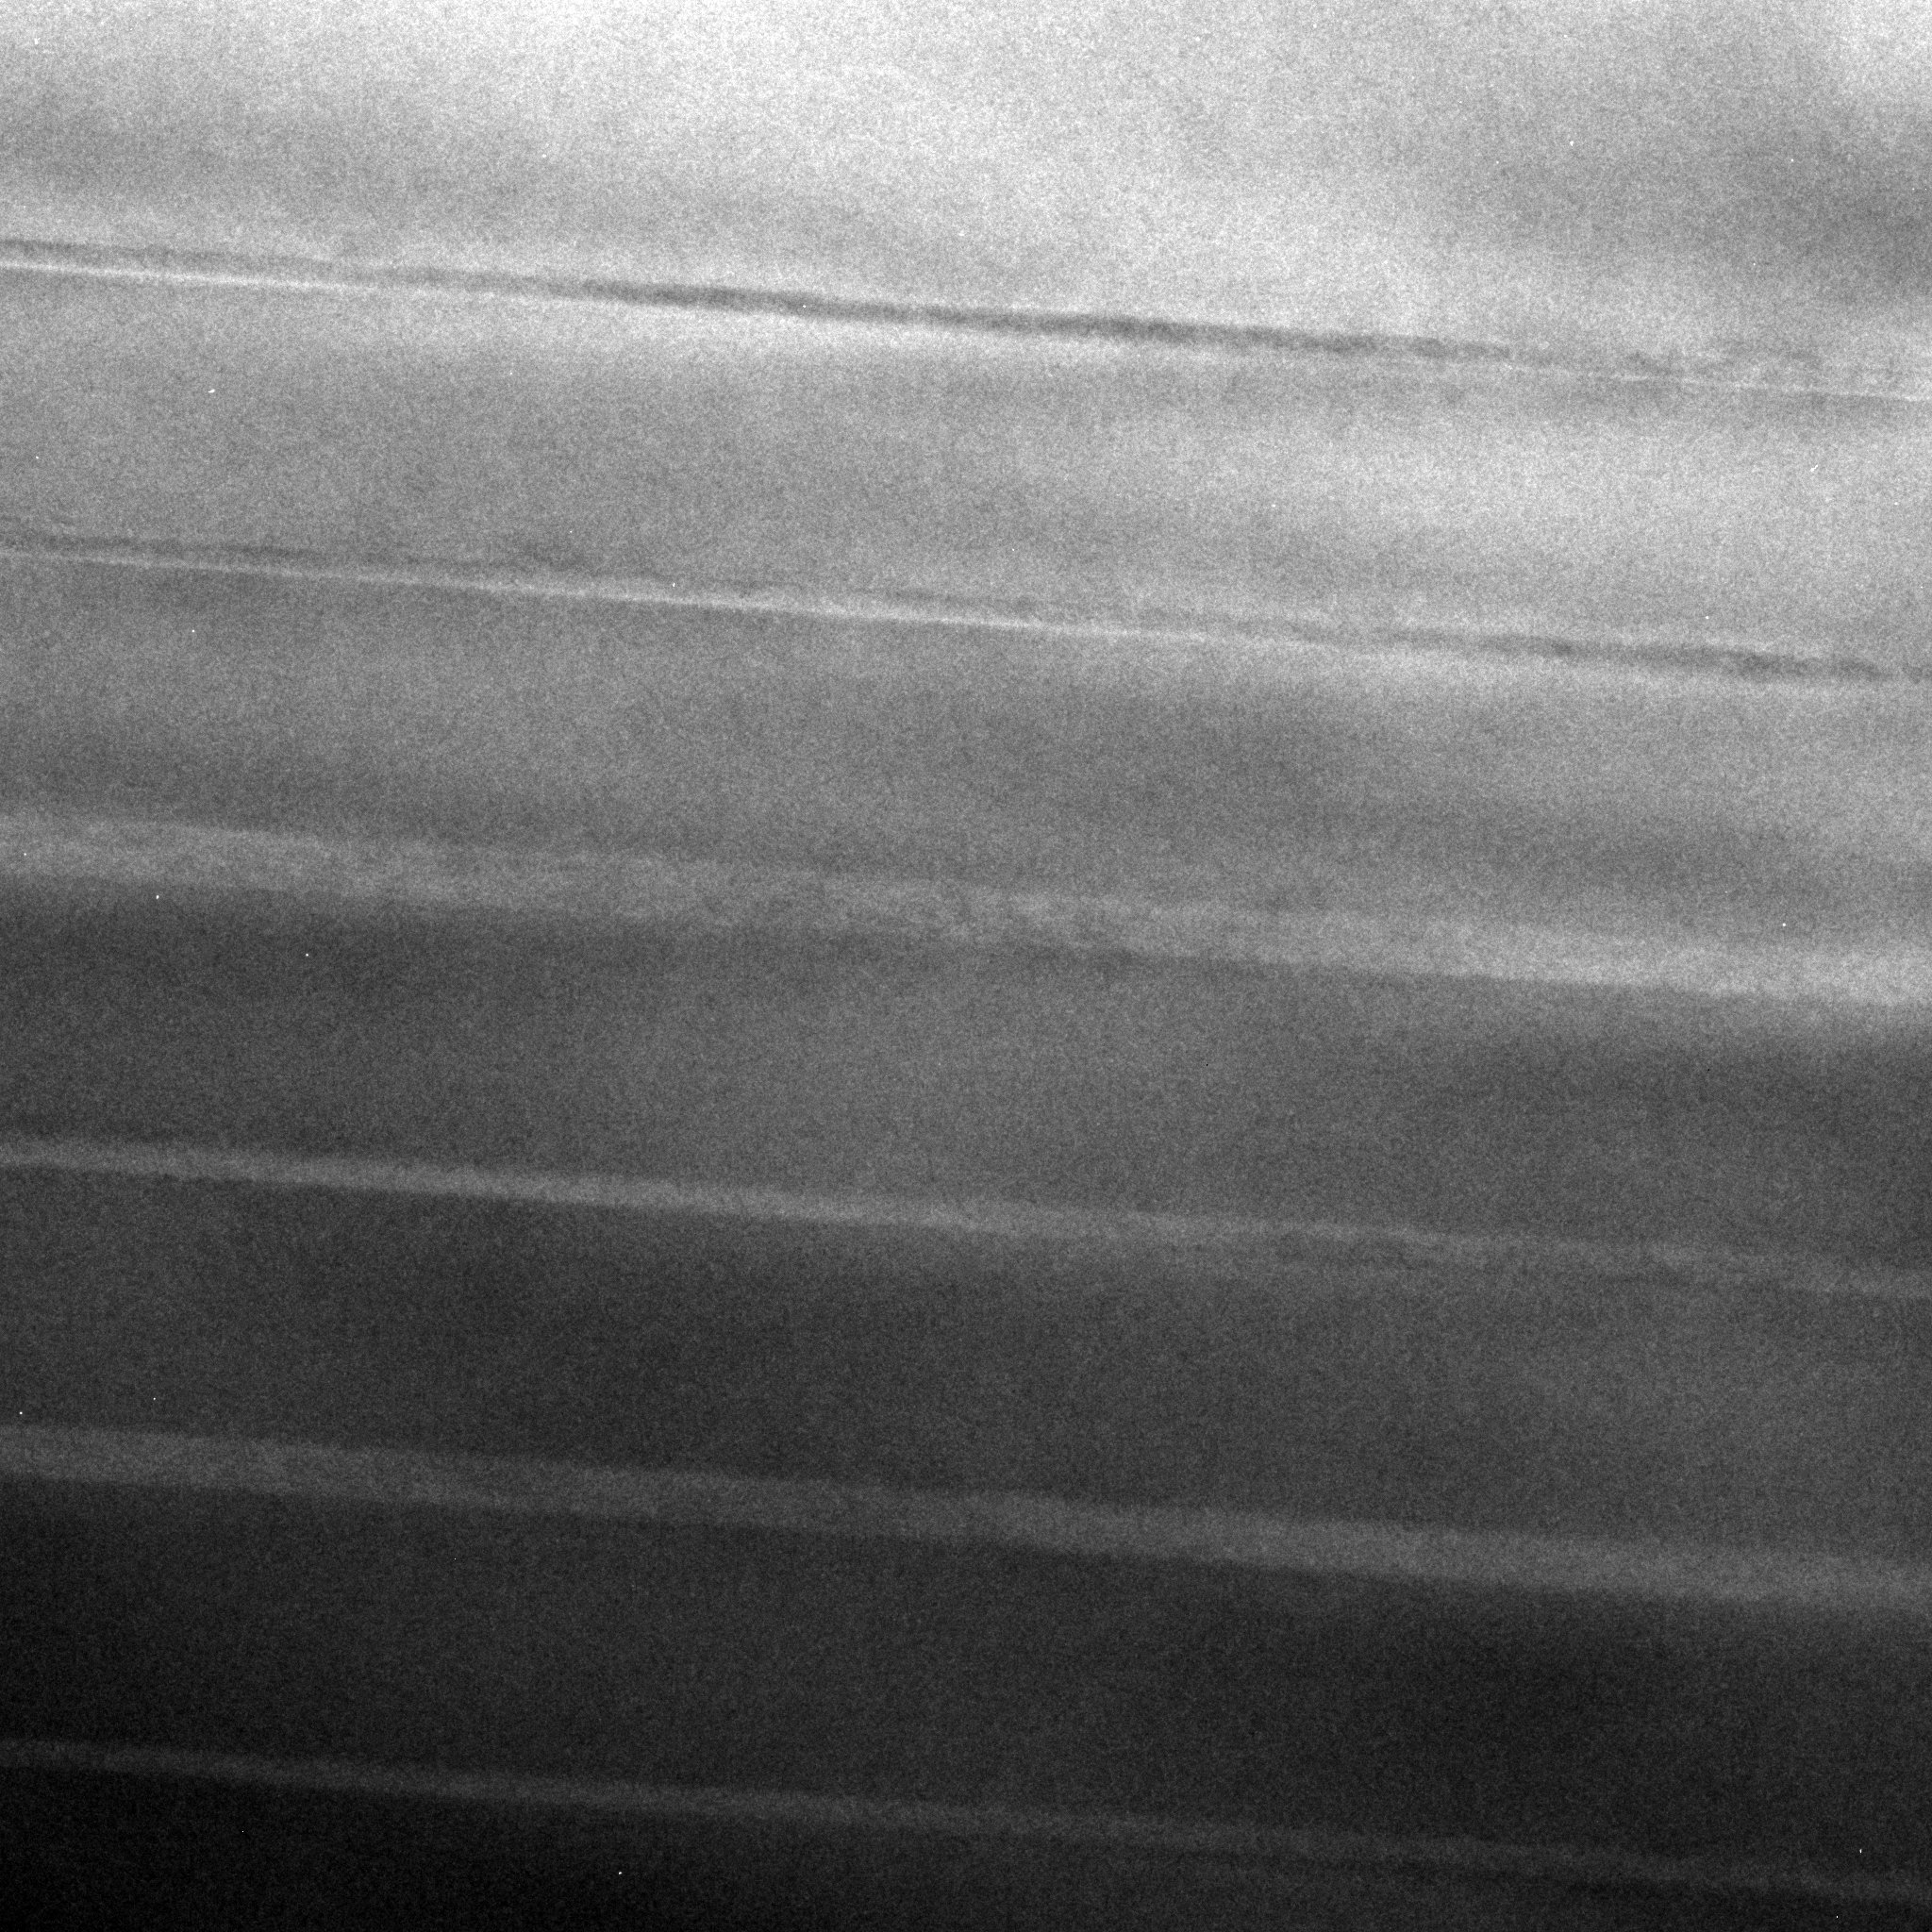
\includegraphics[width=\textwidth]{Grundlagen&Beugung/Eigeneprobe_BF_Quantumbelts_(true)2.jpg }
         \caption{Brightfield}
         \label{EPBFQB}
     \end{subfigure}
     \hfill
     \begin{subfigure}[b]{0.49\textwidth}
         \centering
         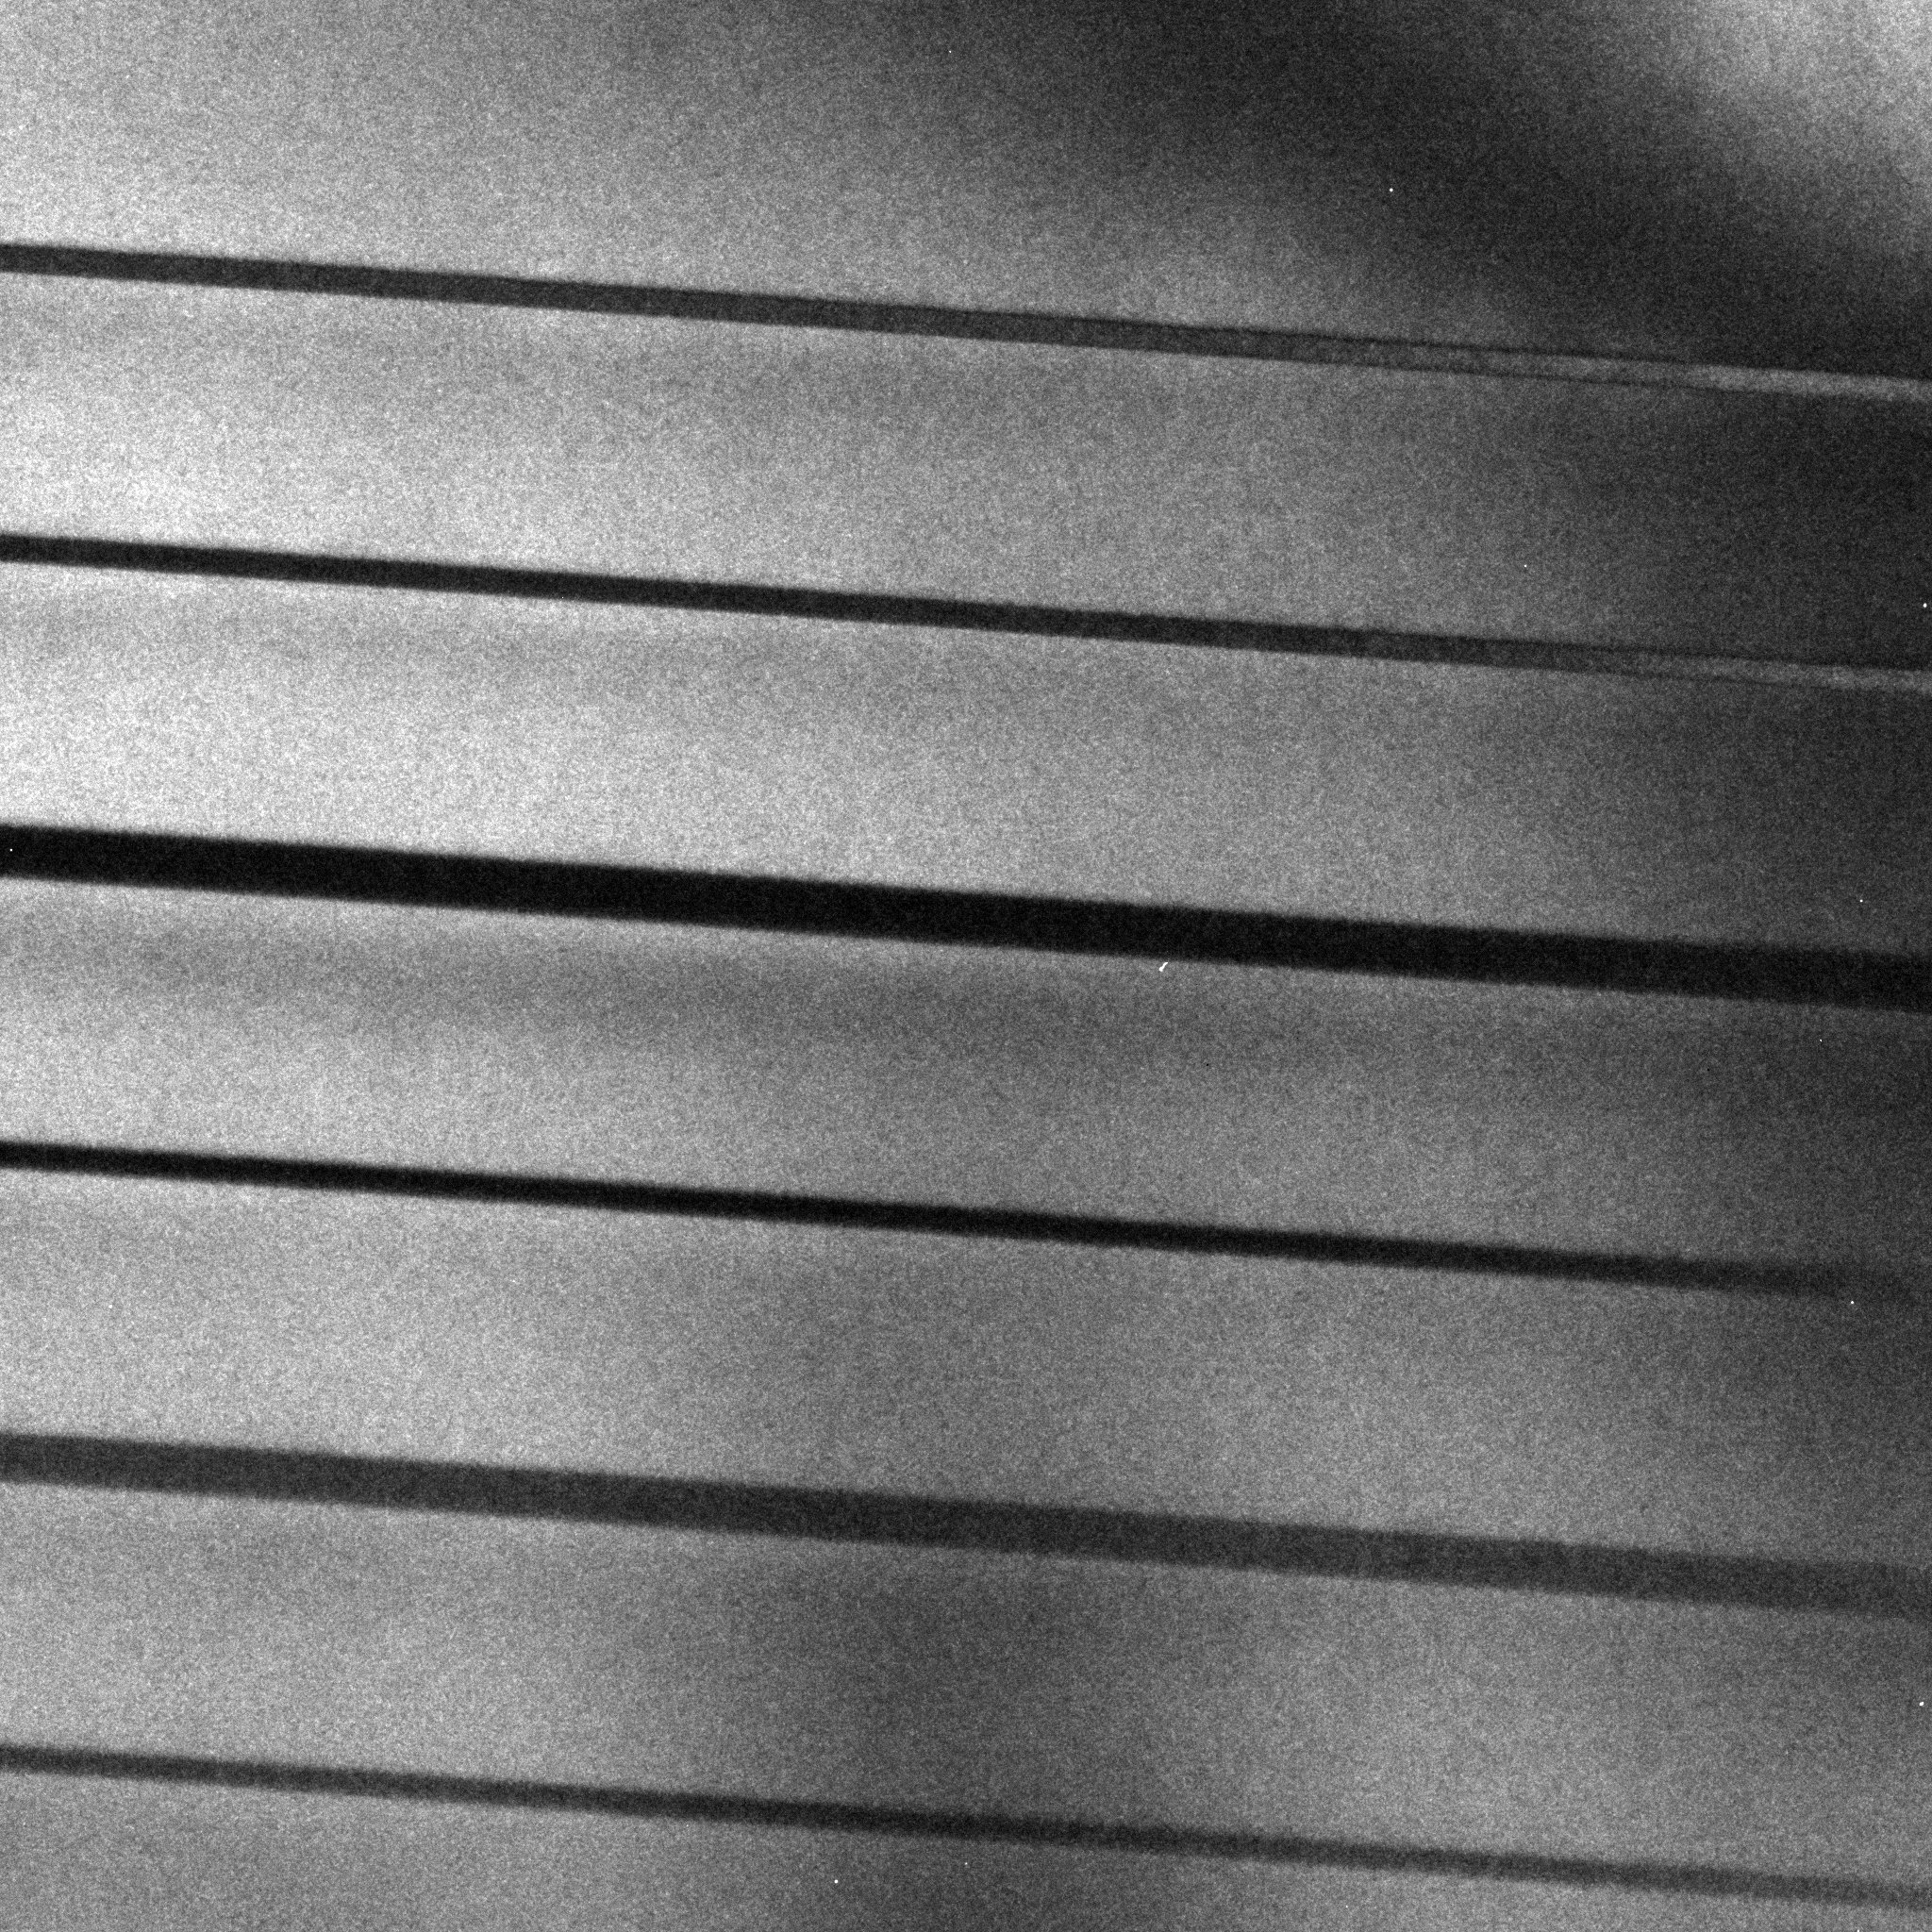
\includegraphics[width=\textwidth]{Grundlagen&Beugung/Eigeneprobe_DF_Quantumbelt_(true)2.jpg}
         \caption{Darkfield}
         \label{EPDFQB}
     \end{subfigure}
        \caption{TEM Darkfield und Brightfield Aufnahme GaAs Probe.}
        \label{EPBF&DFQB}
\end{figure}

\section{Holographie}
In der Elektronen Mikroskopie besteht ein großes Interesse darin einen Phasen Modulation abzubilden, die kann durch eine Elektrostatische und Magnetischen Wechselwirkung entstehen. Um diese Modulation sichtbar zu machen kann sich der Holographie bedient werden. \\
In diesem Versuchsaufbau wurde versucht mit Hilfe von Holographie durch ein Möllenstedt‘sches Biprisma ein P-N Übergang in einem Silizium Chip zu analysieren.

\subsection{Möllenstedt‘sches Biprisma Holographie}
Bei der Holografie mit einem Möllenstedt‘sches Biprisma wird der Elektronenstrahl im TEM Mikroskop durch einen dünnen Quarz-Goldfaden, an dem eine positive Spannung anliegt, in zwei Teilstrahlen aufgespaltet. Ein teilstrahlt durchleuchtet das Objekt und der andere Teilstrahl bleibt ungestört. Die Beiden Teilstrahlen werden wieder vereint und interferieren miteinander auf dem Leuchtschirm/CCD-Kamera. Das dabei entstehende Interferenzmuster stellt das Hologramm da, welches Information der Elektronenwelle enthält, wie Phase und Amplitude.\\
Durch eine anschließende Fast Fourier Transformation Auswertung am Computer kann die Amplitude und Phase zu einem Phasen und Amplitudenbild rekonstruiert werden.

\subsection{Interferenz Kontrast und Beleuchtung}
Der Kontrast des Interferenz Muster im Hologramm ist stark von der Beleuchtung und von den System Parametern anhängig, dabei spielen insbesondere die Biprisma Fadenspannung und Winkelkohärenz eine wichtige Rolle.\\
Bei der Fadenspannung muss zwischen zwei Faktoren abgewogen werden, bei einer hohen Fadenspannung wird eine große Hologramm Breite geschaffen, jedoch singt der Kontrast dabei. Im umgekehrten Fall wird mit einer geringen Fadenspannung eine Schmale Hologramm Breite geschaffen die jedoch einen hohen Kontrast aufweist. \\
Ähnlich ist es bei der Winkelkohärenz, diese wird durch die Aufweitung der Beleuchtung Fläche mit einer Köhler Beleuchtung verändert. Hierbei ist ein stak zusammengezogener strahl kohärenter als ein stark geweiteter Strahl. Durch eine hohe Kohärenz wird dementsprechend auch der Kontrast verbessert. \\
Zusätzlich muss bei der Aufweitung des Strahles zwischen der geringen Anzahl an gemessenen Elektronen bei einer starken Aufweitung des Strahls und einer hohen Anzahl der gemesseneren Elektronen bei einem stak zusammengezogenen Strahl abgewogen werden. Bei einer sehr niedrigen gemessenen Elektronen Zahl ist das Rauschen erhöht und damit auch der Kontrast im Interferenz Muster verringert. \\
Um die Oben aufgeführten Abwägungen zu optimieren kann eine Elliptische Beleuchtung mit Hilfe eines Stigmators verwendet werden. Die Benutzung einer Elliptischen Beleuchtung führt zu einem bestmöglichen Kontrast im Interferenz Muster.

\subsection{Phasenschiebung}
Bei TEM wird die Phasenschiebung eines elektrisches potential beschrieben durch:

\begin{equation}
\begin{split}
\label{eq:PhaseShift}
    & \Delta \varphi =\sigma \cdot \int_{Obj} V \,dz\ = \sigma \cdot t_{Obj} (x,y) \cdot [V_{MIP} + V(x,y)] \\
    & V_{MIP}: Mittleres inneres Potential \\
    & V(x,y): Potentialverteilung \\
    & t_{Obj}: Objektdicke \\
    & \sigma (300kV) = 0,00653 nm^{-1}V^{-1}: Wechselwirkungskonstante \\
    \end{split}
\end{equation}

Dabei können die drei Parameter \(V_{MIP}\), \(V(x,y)\) und \(t_{obj}\) durch die Holografie bestimmt werden. Welche nicht durch die CTEM bestimmt werden können.\\
In unserem Versuch kann \(t_{obj}\) mit eine uniform Dicke angenommen werden, da die Probe durch ein FIB bearbeitet wurde und kann dadurch gegebenen vernachlässigt werden. Durch das Mittlere innere potential ( \(V_{MIP}\)) kann Beispielswiese unterschiedliche Elemente in der Probe bestimmt werden. Die Potential Verteilung (\(V(x,y)\)) hingegen kann Dotierung in der Probe aufzeigen, z.B. von P-N übergangen.\\
Diese Phasenschiebung wird im Phasenbild sichtbar gemacht, eine Amplitudenbild ist dazu nicht in der Lage.

\subsection{Lorenzmodus/Lorentz Mikroskopie}
% Dieser teil muss vieleicht nochmal ueberarbeitet werden
Ein Kontrast entsteht durch die Ablenkung der Elektronen durch elektrische und magnetische Strukturen im Objekt. Durch die Ablenkung entstehen konvergente und divergente Regionen die dementsprechend die Phase und Amplitude modulieren. Bei der Lorentz Mikroskopie muss eine parallele Beleuchtung verwendet werden.
%%Nochmal Ueberarbeiten!!!!!

\subsection{Experiment}
\subsubsection{Leerhologramme}
Für die Holographie Experimente muss zuerst das Titan Mikroskop hochgefahren werden und eingestellt werden. Dieser Prozess ist zum Großteil analog zum zuvor behandelten CTEM teil.\\
Dies Beinhaltet:
\begin{itemize}
\item Vakuum Checkt (Octagon < 20Log)
\item Hochspannung Check \( (U_A = 300kV) \)
\item Schleusen Öffnen
\item Im Low Magnification Modus die Probe in den Messbereich verfahren
\end{itemize}

Anschließend muss das Biprisma in den Elektronenstrahl verfahren werden und durch die manuellen Verschiebungsregler muss der Faden in das Zentrum des den Elektronenstrahl gebracht werden. Zusätzlich wird die Kondensor Linse 3 eingeschaltet. Das Titan ist mit 3 Biprisma ausgestattet, es wird jedoch nur das Biprisma 1 in diesem Versuchen verwendet. \\
Das Mikroskop wird anschließend in den Lorentz Modus gestellt und eine Spannung auf den das Biprisma gelegt. Nach dem das Biprisma Thermisch stabil ist werden alle Linsen Normalisiert „Normalize all“, mit Hilfe des „Beam Shift“ und des „Reset Beam“ wird der Offset wieder zum Zentrum des Bildes gefahren. Anschließend wird analog zum TEM-Teil der Strahl mit dem Stigmator rund geformt und der Pivot Point eingestellt werden. \\
Als erstes wurde ein Leer Hologramm erstellt, also ohne das eine Probe/Objekt im Strahlengang einsetzt wurde. Dabei wurde eine Fadenspannung von 70V angelegt.Siehe Abbilung \cref{698VakRund}. Das entstehende Interferenzmuster zeigt eine symmetrische Streifenverteilung auf. Es sind zusätzlich Fresnel-Beugungstreifen zu erkennen, diese sind an den Außenseiten des Hologramms festzustellen, sie haben einen niedrigeren Kontrast und eine größer Streifenbreite als die Hologramm-Interferenzstreifen. Außerdem ist die Streifenbreiten nicht homogen wie bei dem Hologramm streifen. (siehe Abbildung \cref{VakHolRund})
Um eine Optimale Fadenspannung für ein Hologramm zu finden wurden Leerhologramme mit Fadenspannung von 0V bis 90V in 10V schritten erstellt.

\begin{figure}[H]
     \centering
     \begin{subfigure}[b]{0.49\textwidth}
         \centering
         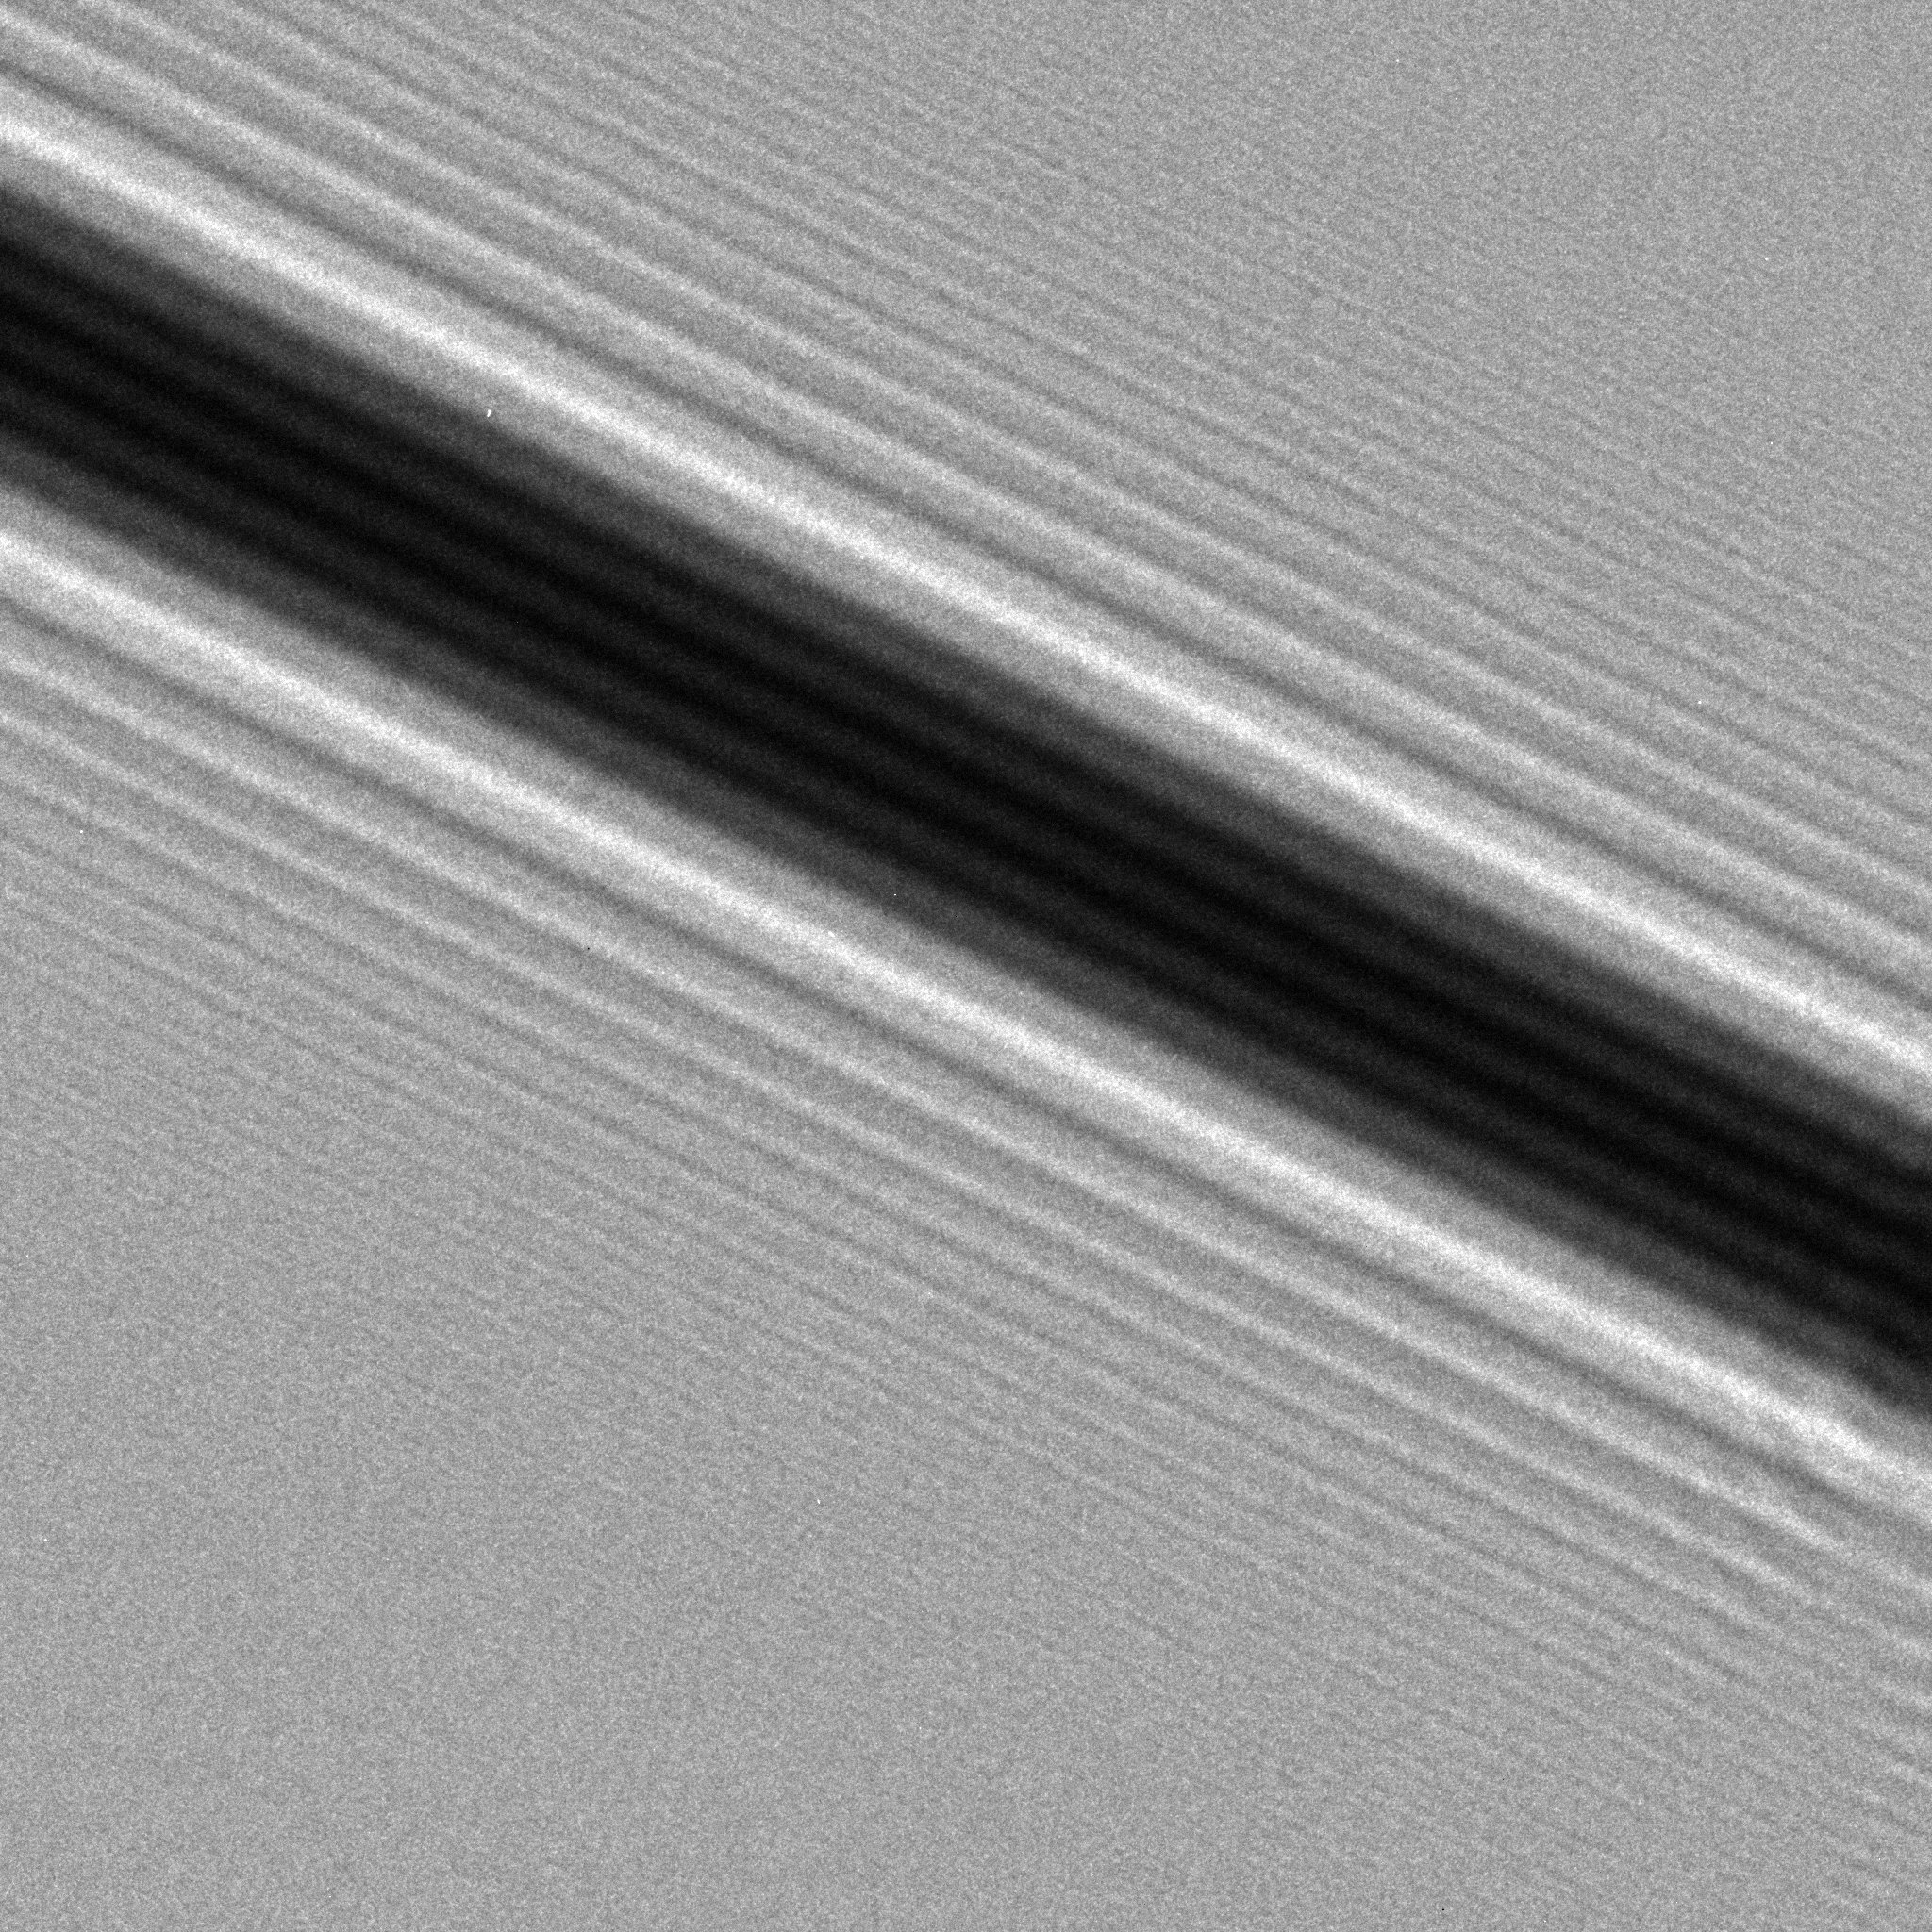
\includegraphics[width=\textwidth]{Holographie/Vakuumhologramm_Rundbeleuchtung/0_02_Vak_Rund.jpg}
         \caption{\(U_F =\) 0,02V}
         \label{002VakRund}
     \end{subfigure}
     \hfill
     \begin{subfigure}[b]{0.49\textwidth}
         \centering
         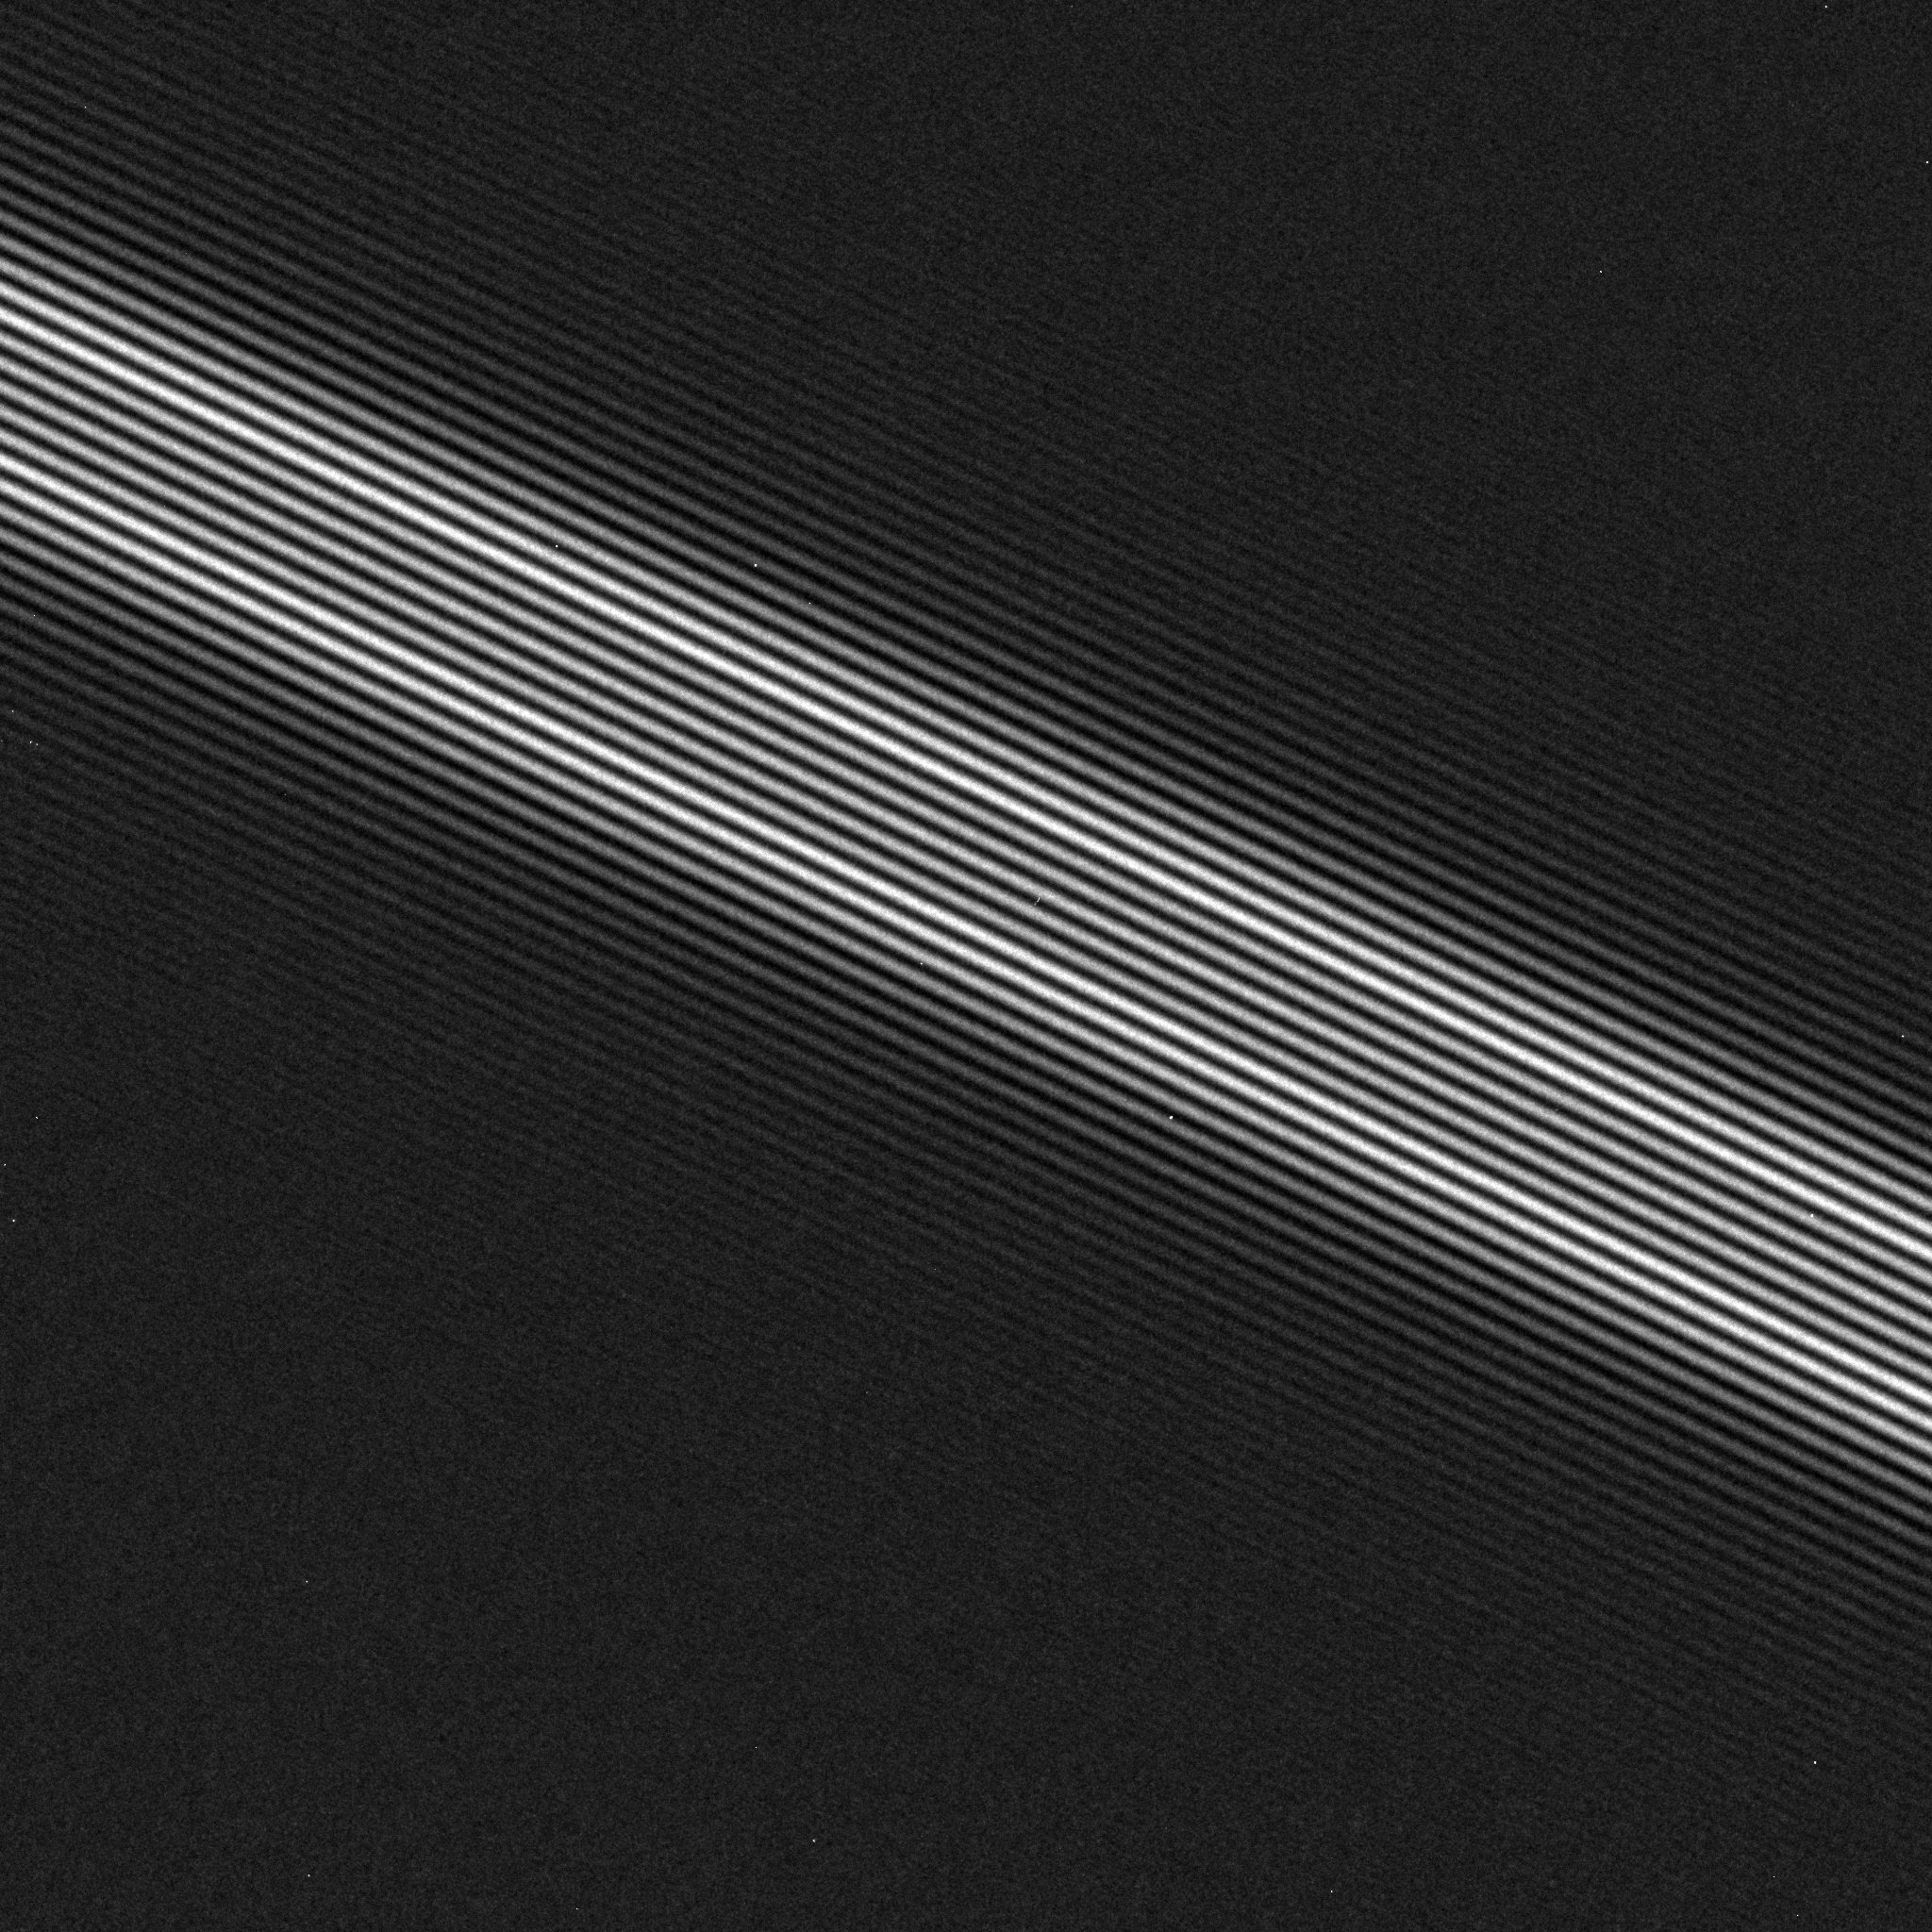
\includegraphics[width=\textwidth]{Holographie/Vakuumhologramm_Rundbeleuchtung/20_4_Vak_Rund.jpg}
         \caption{\(U_F =\) 20,4V}
         \label{204VakRund}
     \end{subfigure}
      
 %\vspace{}

 \centering
     \begin{subfigure}[b]{0.49\textwidth}
         \centering
         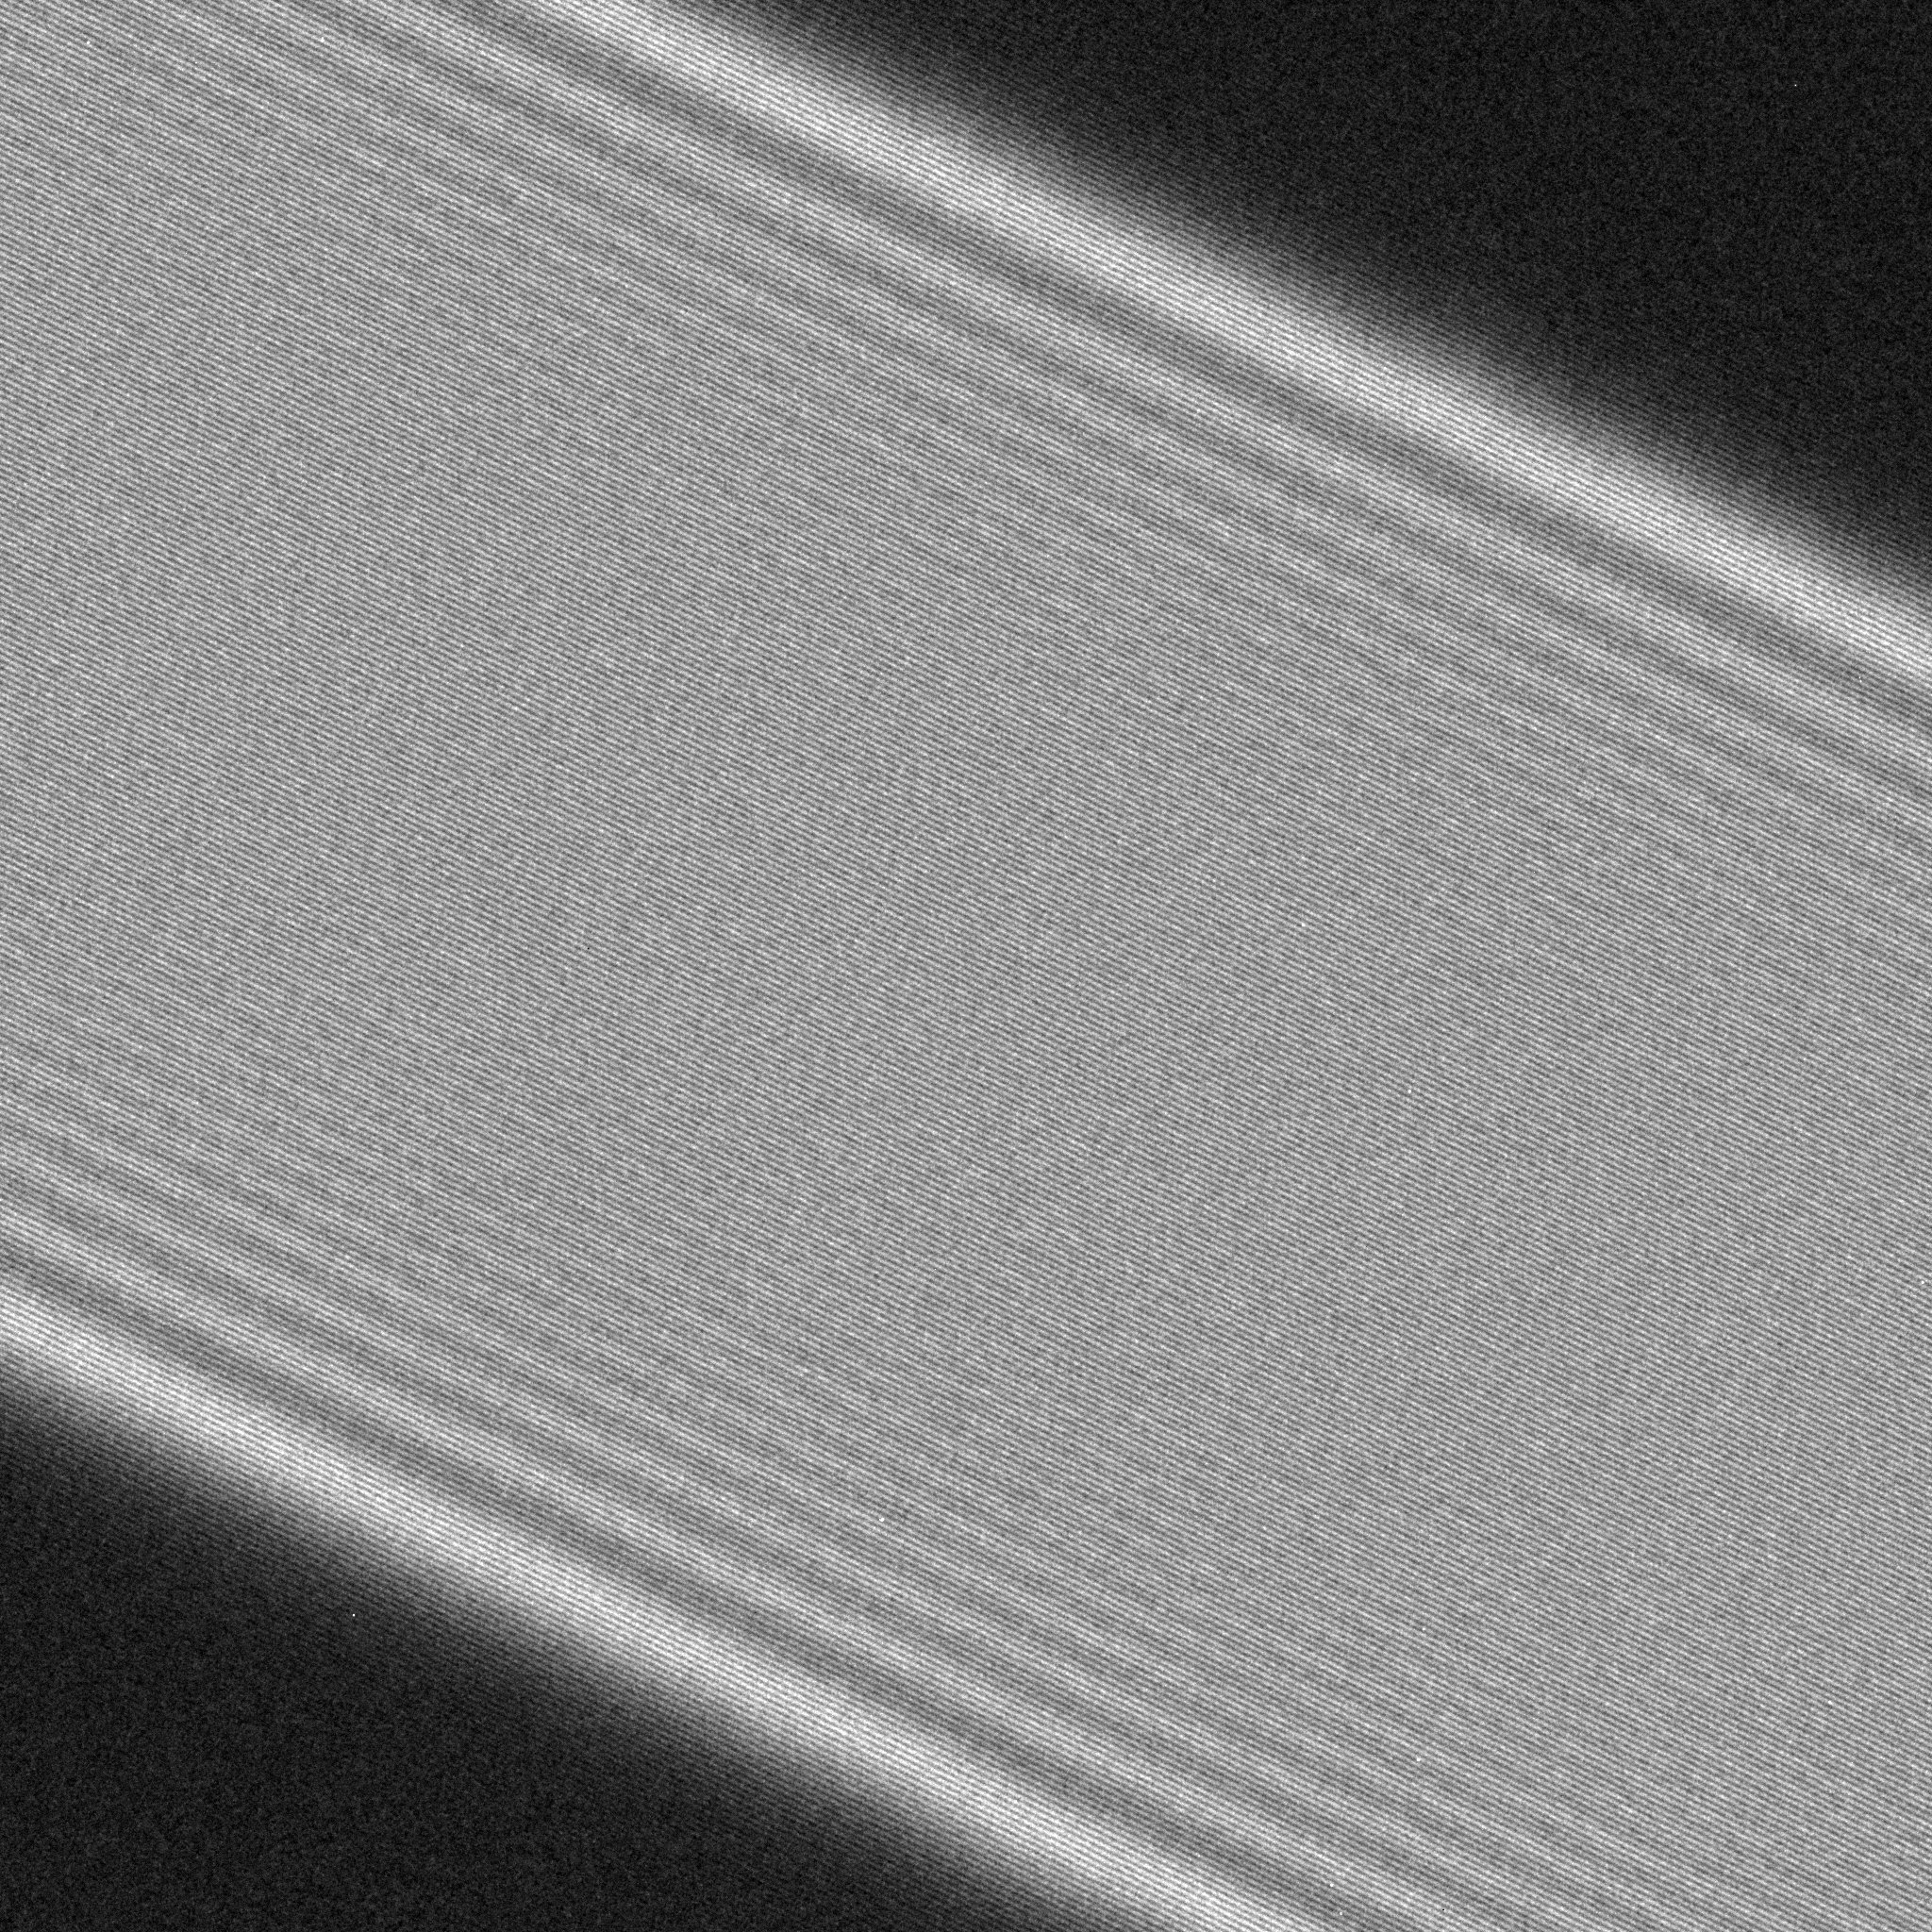
\includegraphics[width=\textwidth]{Holographie/Vakuumhologramm_Rundbeleuchtung/69_8_Vak_Rund.jpg}
         \caption{\(U_F =\) 69,8V}
         \label{698VakRund}
     \end{subfigure}
     \hfill
     \begin{subfigure}[b]{0.49\textwidth}
         \centering
         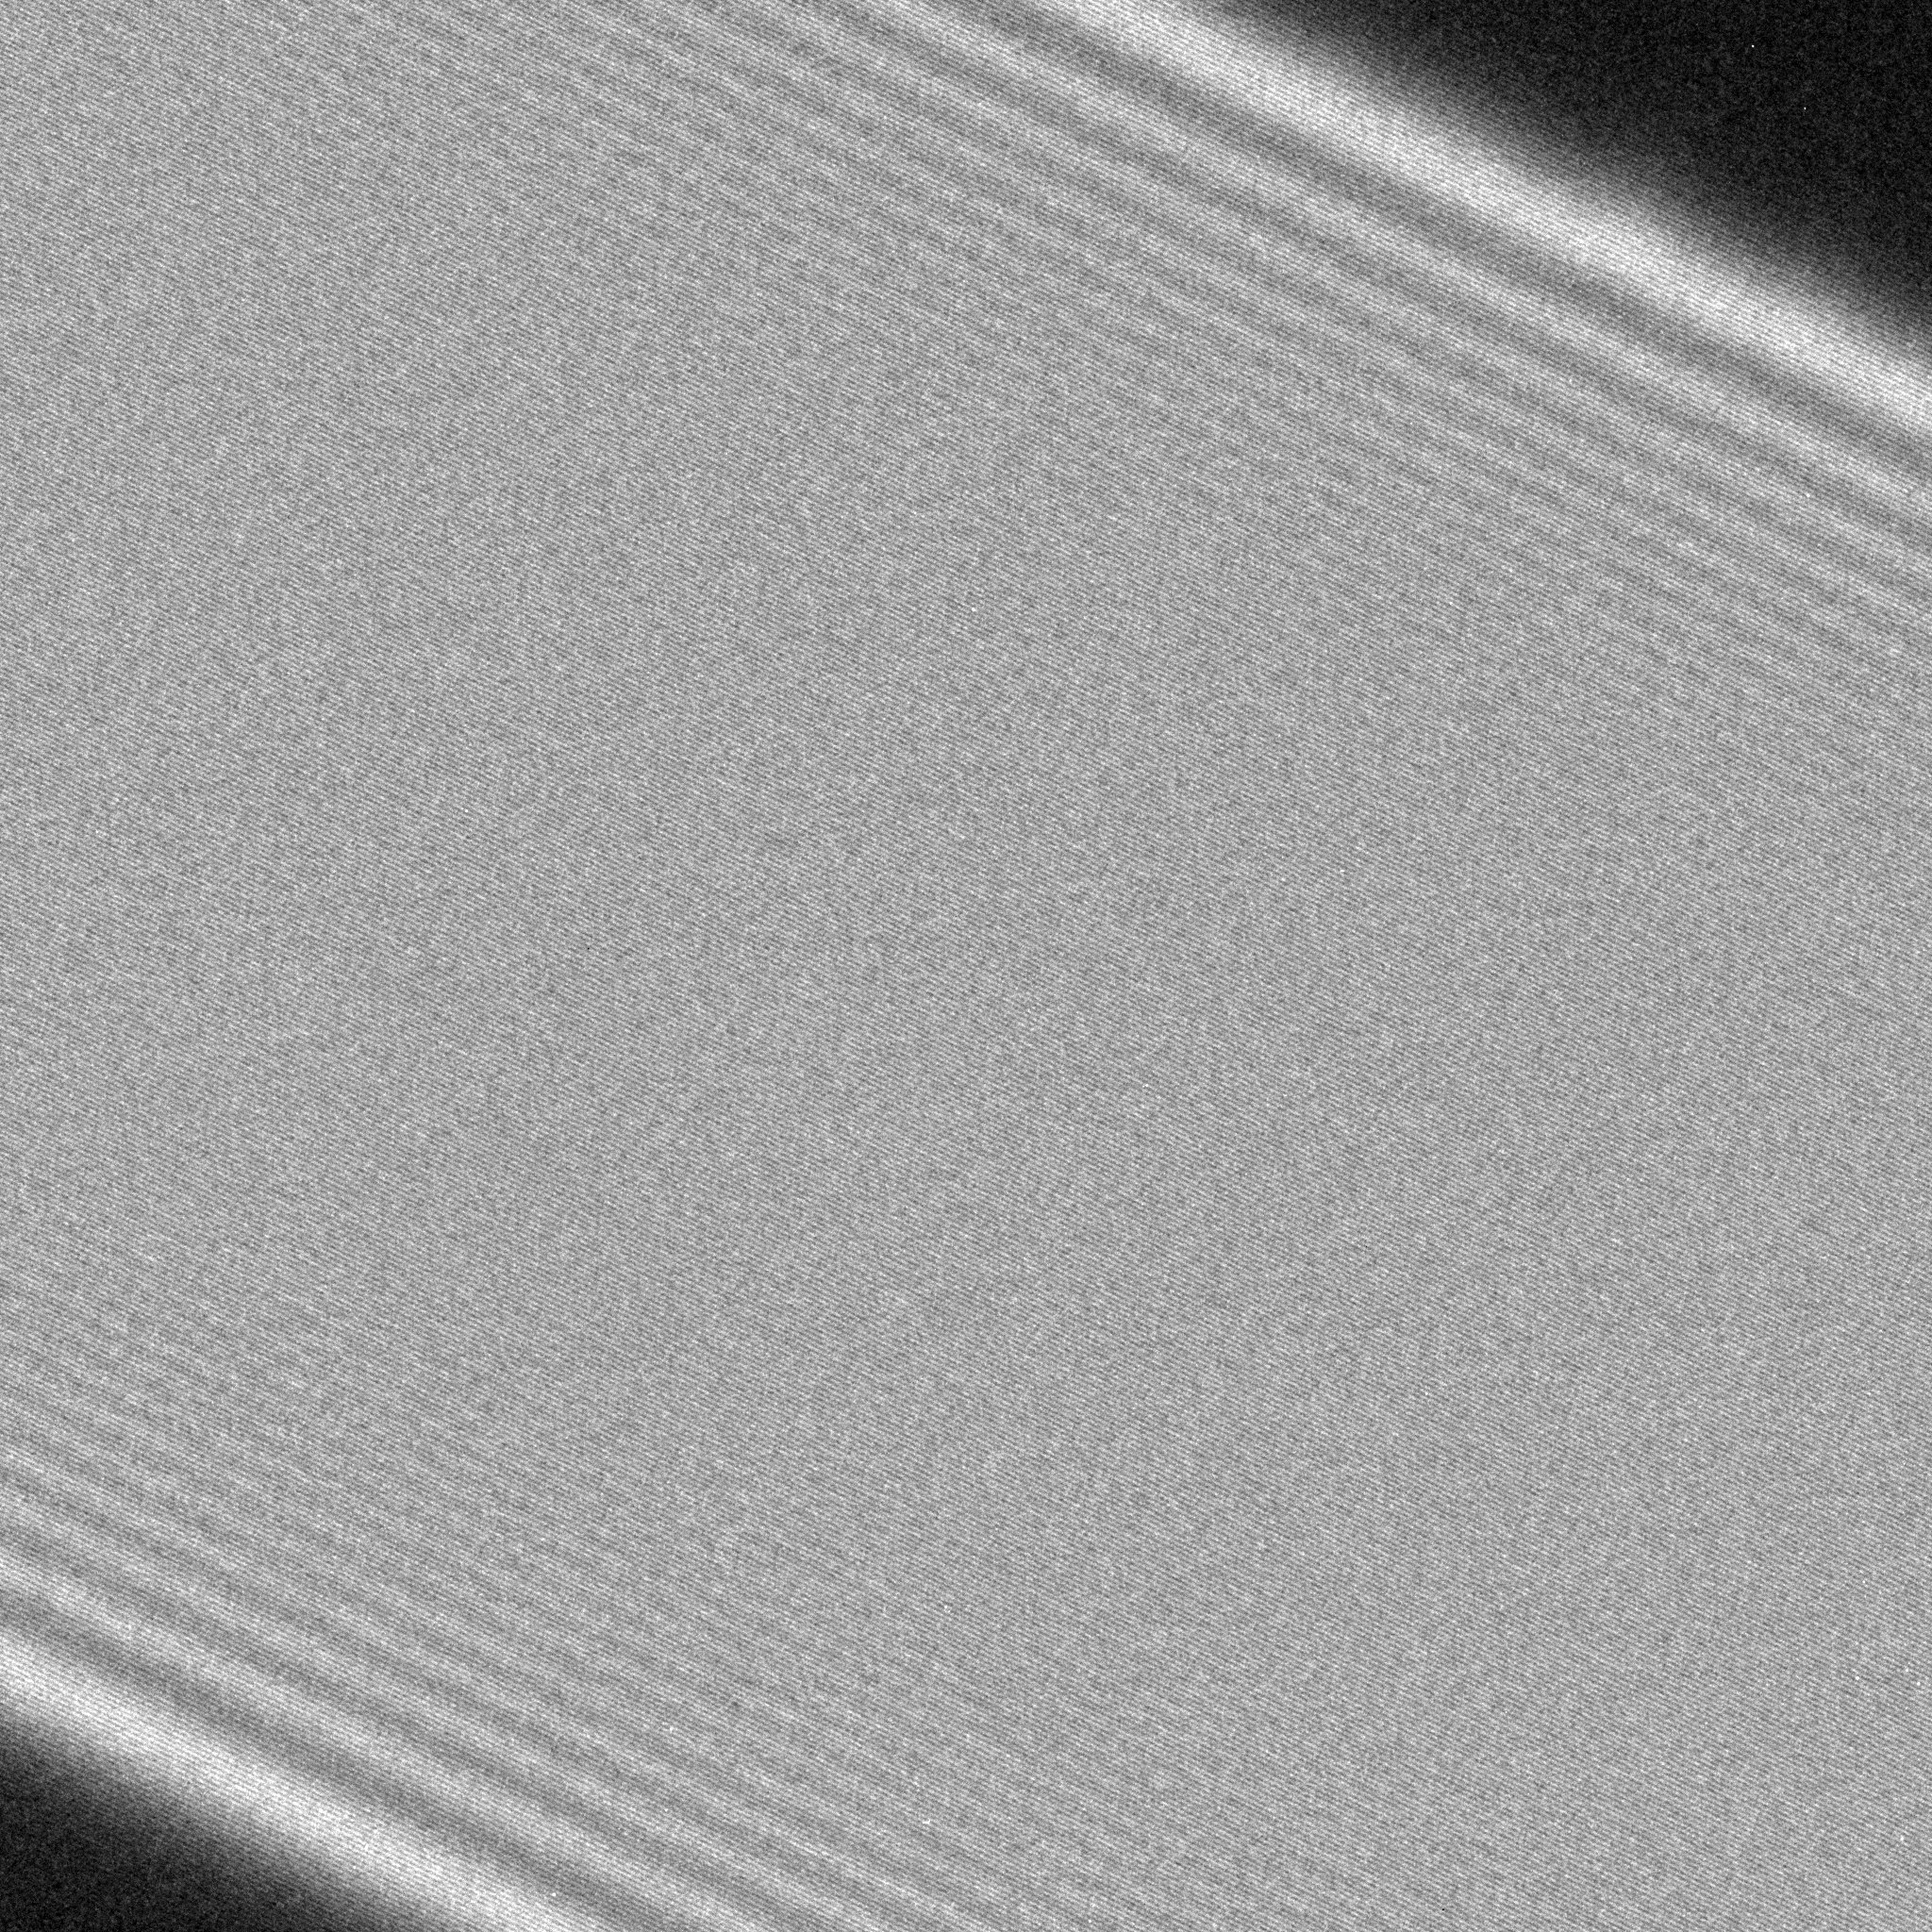
\includegraphics[width=\textwidth]{Holographie/Vakuumhologramm_Rundbeleuchtung/90_4_Vak_Rund.jpg}
         \caption{\(U_F =\) 90,4V}
         \label{904VakRund}
     \end{subfigure}
     \caption{Leerhologramm mit Rundbeleuchtung bei verschiedenen Fadenspannungen}
        \label{VakHolRund}
 
\end{figure}

Bei der Aufnahme ohne eine anliegende Fadenspannung, siehe Bilder \cref{002VakRund}, wird nur leichte Interferenz zwischen den beiden Teilwellen abgebildet, es ist vorallem   Fresnel-Beugung zu sehen. Es ist zusätzlich der durch den Faden verdeckte Elektonenstrahl als Schatten zu erkennen.\\
Bei den Aufnahmen mit einer anliegenden Spannung kann man erkenne das der Interferenzbereich mit zunehmender Spannung größer wird, aber die Interfenz streifen schmaler werden und an Kontrast verlieren. An äußeren Rand des Interferenz Muster kann man weiterhin das Fresnel-Beugung Muster erkennen. \\
Um diese Hologramm Parameter zu quantifizieren wurde ein Skript verwendet, welches in der Lage ist den Streifenkontrast an 5 Punkten der Aufnahme zu messen und angezeigt. Die Interferenzmusterbreite wurde mit der Auswertungssoftware „ImageJ“ gemessen. 

In der Tabelle \cref{VakHolParameter} und den Graphen \cref{VakHolGraph} ist gut zu erkennen wie der Streifenabstand sich mit der Fadenspannung verändert. Die Hologrammbreite nimmt nahezu linear mit der Fadenspannung zu, so wie es durch die Funktion \cref{eq:Hologrammbreite} zu erwarten ist. 

\begin{equation}
\label{eq:Hologrammbreite}
    w_{hol} = 2b \gamma_0 U_F - 2 r_F \frac{a+b}{a}
\end{equation}

\begin{table}[!ht]
    \centering
    \caption{Tabelle der Hologramm Parameter (Steifenabstand, Kontrast und Hologrammbreite) bei unterschiedlichen Biprisma Fadenspannung}
    \begin{tabular}{|l|l|l|l|l|l|l|}
    \hline
        \textbf{Fadenspannung [V]} & \multicolumn{2}{|c|}{\textbf{Kontrast [\%]}} & \multicolumn{2}{|c|}{\textbf{Steifenabstand [Pix]}} & \multicolumn{2}{|c|}{\textbf{Breite [Pix]}} \\ \hline
        \textbf{Beleuchtung:} & Rund & Eliptisch & Rund & Eliptisch & Rund & Eliptisch \\ \hline
        \textbf{0} & 0.62 & 0.92 & 17.7 & 18.25 & 0 & 0 \\ 
        \textbf{10} & 0.35 & 4.5 & 9.17 & 18.29 & 295.945 & 275.476 \\ 
        \textbf{20} & 0.35 & 40.04 & 18.24 & 15.7 & 334.632 & 399.259 \\ 
        \textbf{30} & 37.67 & 31.77 & 15.46 & 11.91 & 419.34 & 517.229 \\ 
        \textbf{40} & 29.2 & 31.36 & 12.08 & 11.76 & 525.395 & 541.194 \\ 
        \textbf{50} & 22.18 & 25.16 & 9.53 & 9.69 & 643.836 & 654.702 \\ 
        \textbf{60} & 17.19 & 20.26 & 8.12 & 7.95 & 796.13 & 816.493 \\ 
        \textbf{70} & 13.62 & 16.45 & 6.99 & 6.96 & 914.647 & 931.022 \\ 
        \textbf{80} & 10.46 & 12.34 & 6.08 & 6.04 & 1104.862 & 1098.322 \\ 
        \textbf{90} & 7.65 & 10.14 & 5.41 & 5.42 & 1261.25 & 1228.854 \\ \hline
    \end{tabular}
    \label{VakHolParameter}
\end{table}

\begin{figure}
     \centering
     \begin{subfigure}[b]{0.3\textwidth}
         \centering
         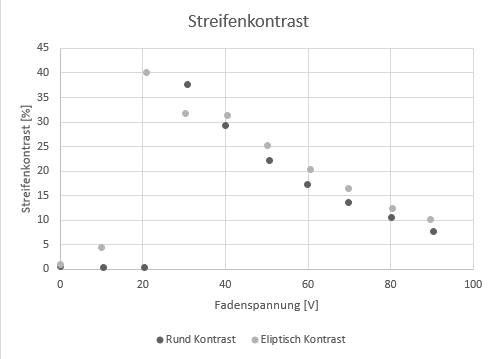
\includegraphics[width=\textwidth]{Holographie/Vakuumhologramm_Rundbeleuchtung/Kontrast.png}
         \caption{Kontrast}
         \label{LeerHolKontrast}
     \end{subfigure}
     \hfill
     \begin{subfigure}[b]{0.3\textwidth}
         \centering
         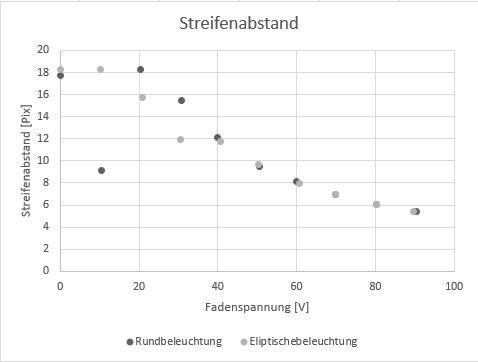
\includegraphics[width=\textwidth]{Holographie/Vakuumhologramm_Rundbeleuchtung/Streifenabstand.png}
         \caption{Streifenabstand}
         \label{LeerHolStreifenabstand}
     \end{subfigure}
     \hfill
     \begin{subfigure}[b]{0.3\textwidth}
         \centering
         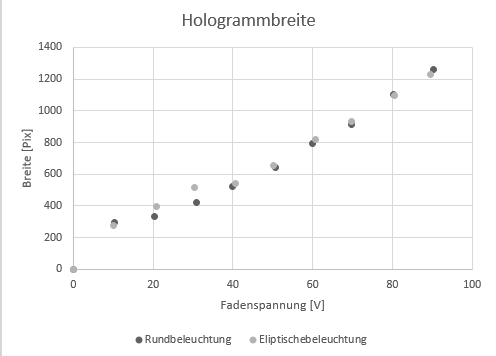
\includegraphics[width=\textwidth]{Holographie/Vakuumhologramm_Rundbeleuchtung/Hologrammbreite.png}
         \caption{Hologrammbreite}
         \label{StreifenabstandBreite}
     \end{subfigure}
        \caption{Plots der Steifenabstand, Kontrast und Hologrammbreite in Leerhologrammen bei Rund und Elliptischer Beleuchtung für verschiedene Fadenspannungen}
        \label{VakHolGraph}
\end{figure}

Der streifenabstand hingegen wird durch Formel \cref{Streifenabstand} beschriebenen und gibt eine inversproportionale Abhängigkeit von der Fadenspannung an. Diese kann auch beobachtet werden, jedoch nicht bei geringeren Fadenspannung

\begin{equation}
\label{Streifenabstand}
    s_{hol} = \frac{1}{q_c} = \frac{a+b}{2 k a \gamma_0 U_F}
\end{equation}

Der Kontrast hat seinen Maxima bei einer Fadenspannung von ca. 30V mit einer runden Beleuchtung und 20V bei der elliptischen Beleuchtung. Auf die Kontrast Abhängigkeit von Fadenspannung und Beleuchtung wird oben weiter eingegangen.\\
Um den Streifenkontrast des Hologramms zu erhöhen, wurde nun die Beleuchtung von der runden Beleuchtung auf eine elliptische Beleuchtung umgestellt. Dafür wurde die Stigmator Einstellungen so angepasst das der Elliptisch geformte Strahl senkrecht zur Biprisma Faden stand. Durch den stärker zusammengezogenen Strahl und die dadurch entstandenen höheren gemessenen Elektronen Zahl auf dem CCD-Kamera, musste die Beleuchtungszeit auf der Kamera auf 2 Sekunden verkürzt werden, um Überbelichtung zu vermeiden.

Anschließend wurde die Messreihe mit verschiedenen Fadenspannung analog zur rund Beleuchtung für eine Elliptische Beleuchtung widerholt. Siehe Abbildung \cref{VakHolEllip} Im Vergleich zur runden Beleuchtung ist jetzt ein sehr viel besserer Streifenkontrast zu erkennen. 
In der \cref{VakHolParameter} sind sie Ergebnisse zusammengefast, um Graphen \cref{VakHolGraph} dargestellt.

\begin{figure}[H]
     \centering
     \begin{subfigure}[b]{0.49\textwidth}
         \centering
         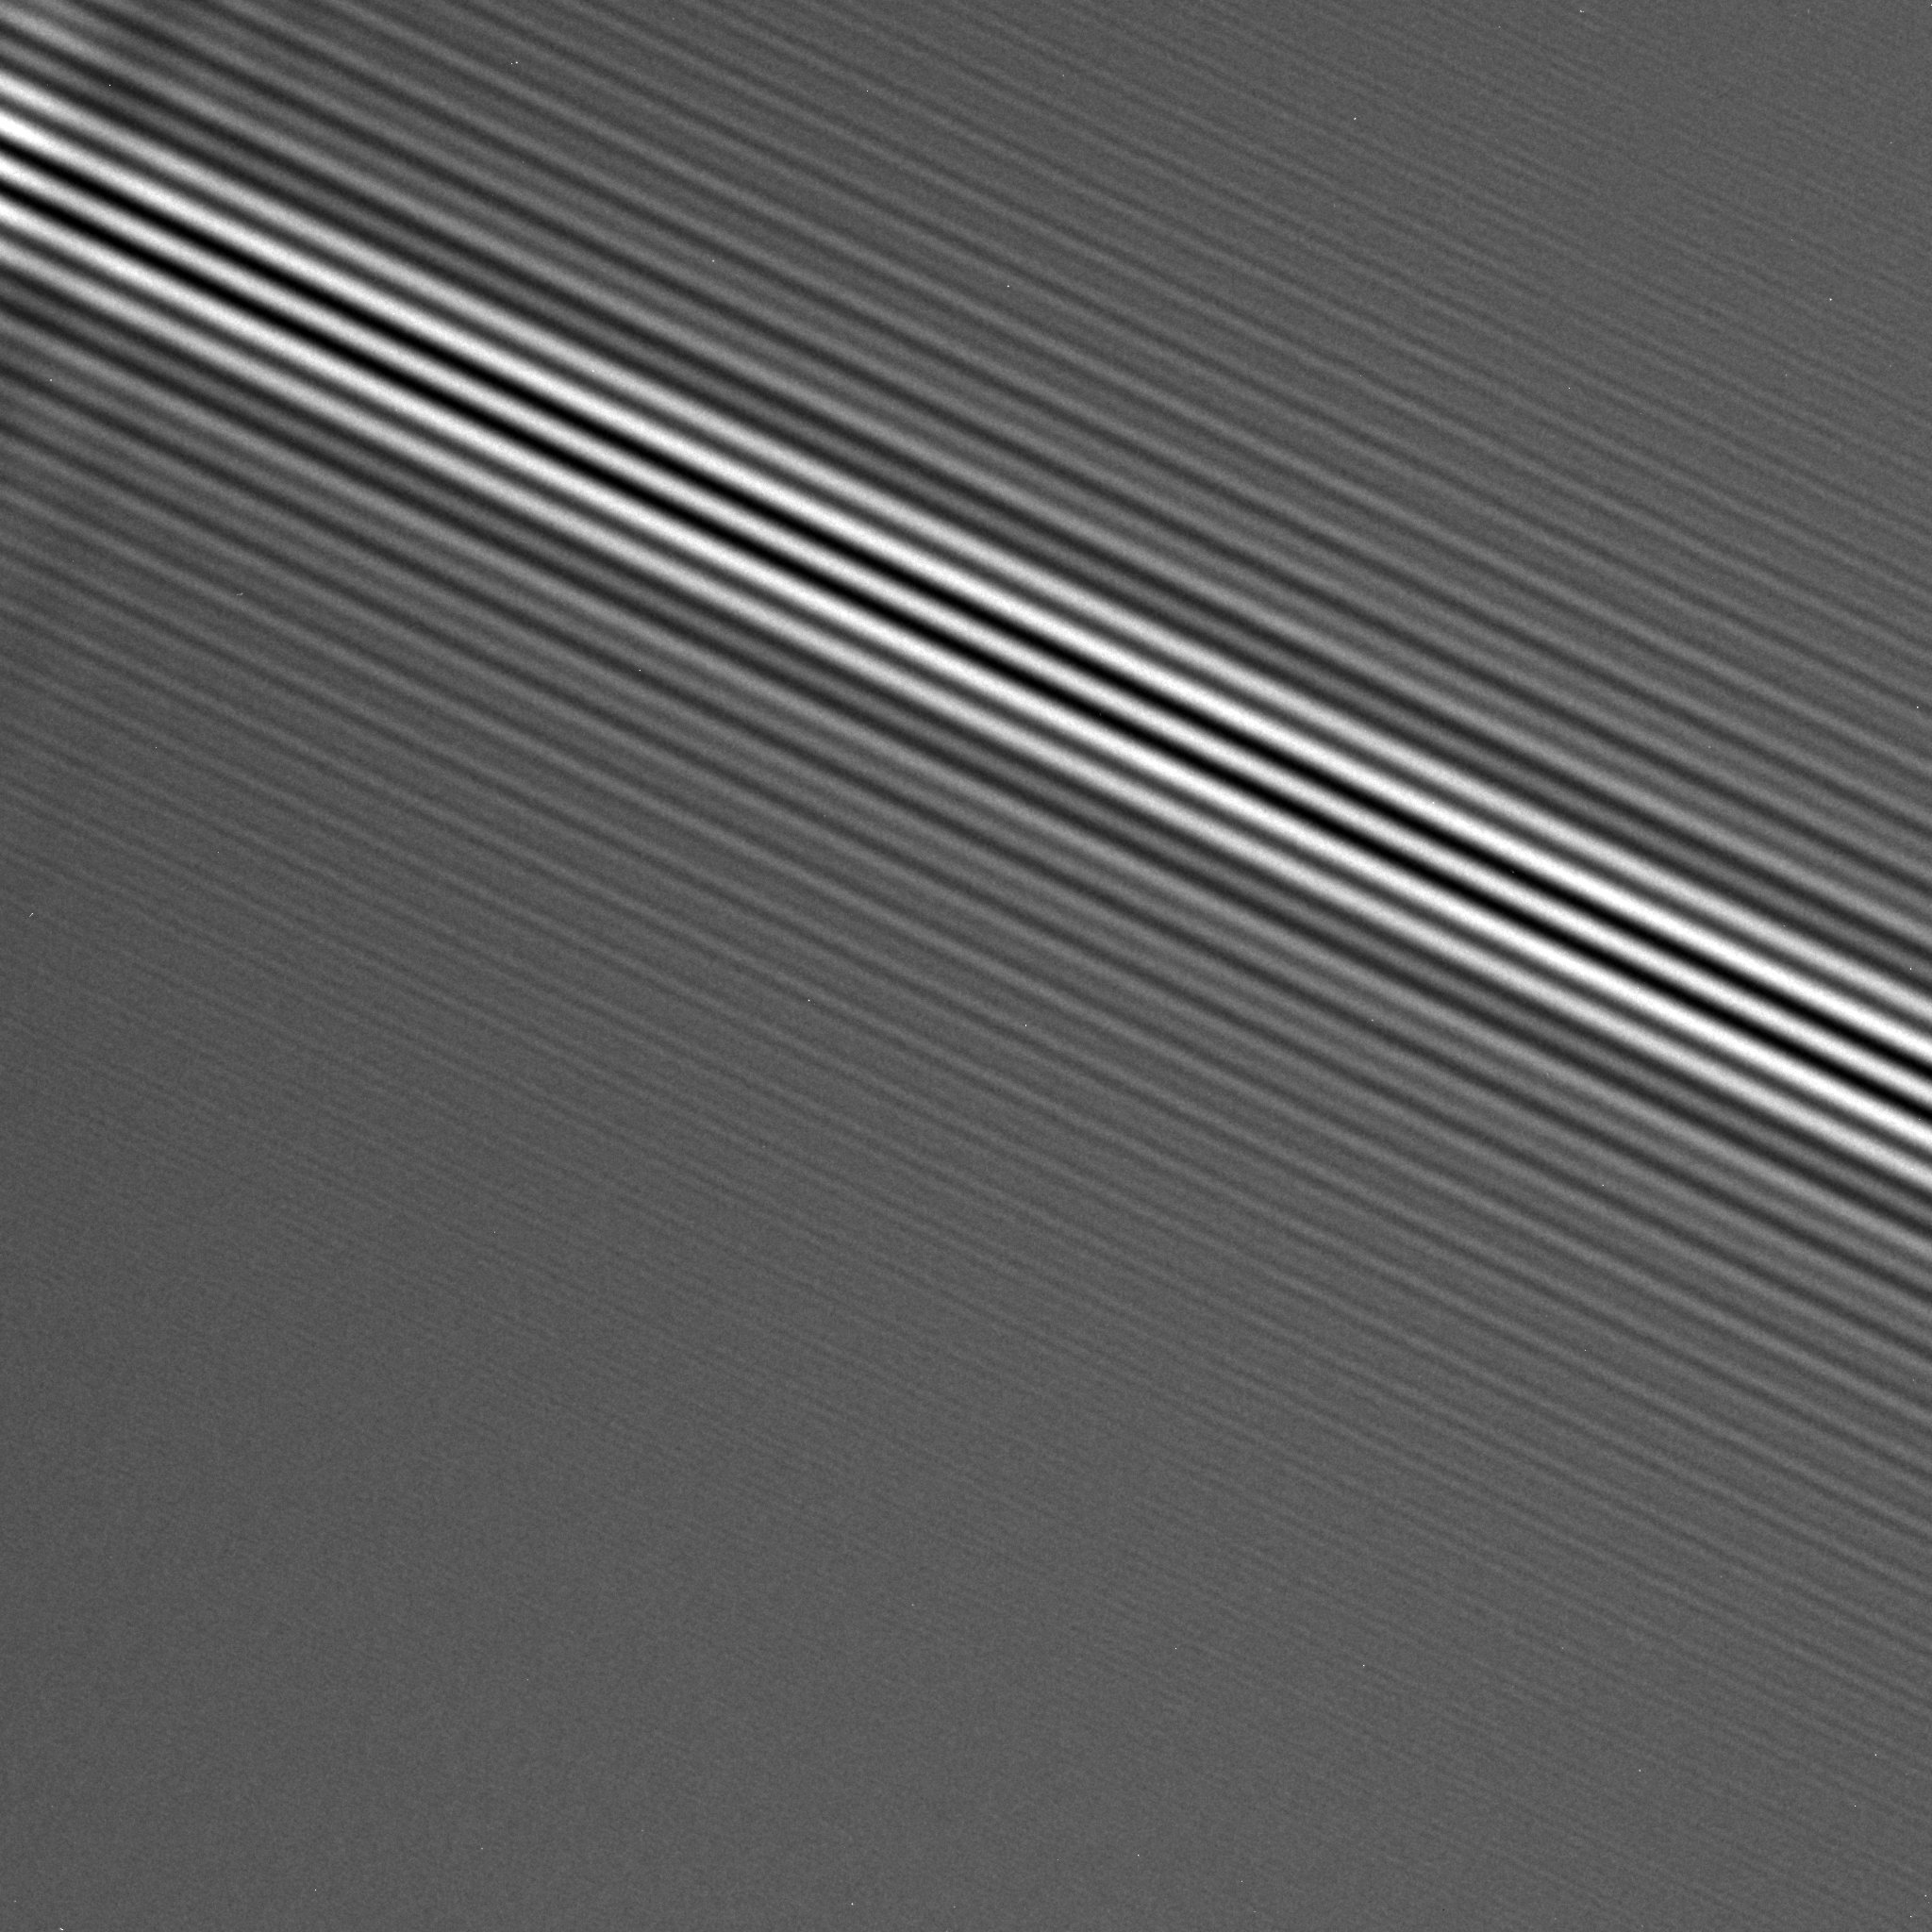
\includegraphics[width=\textwidth]{Holographie/Vakuumhologramm_Elliptischebeleuchtung/0_02_Vak_Ellip.jpg}
         \caption{\(U_F =\) 0,02V}
         \label{002VakEllip}
     \end{subfigure}
     \hfill
     \begin{subfigure}[b]{0.49\textwidth}
         \centering
         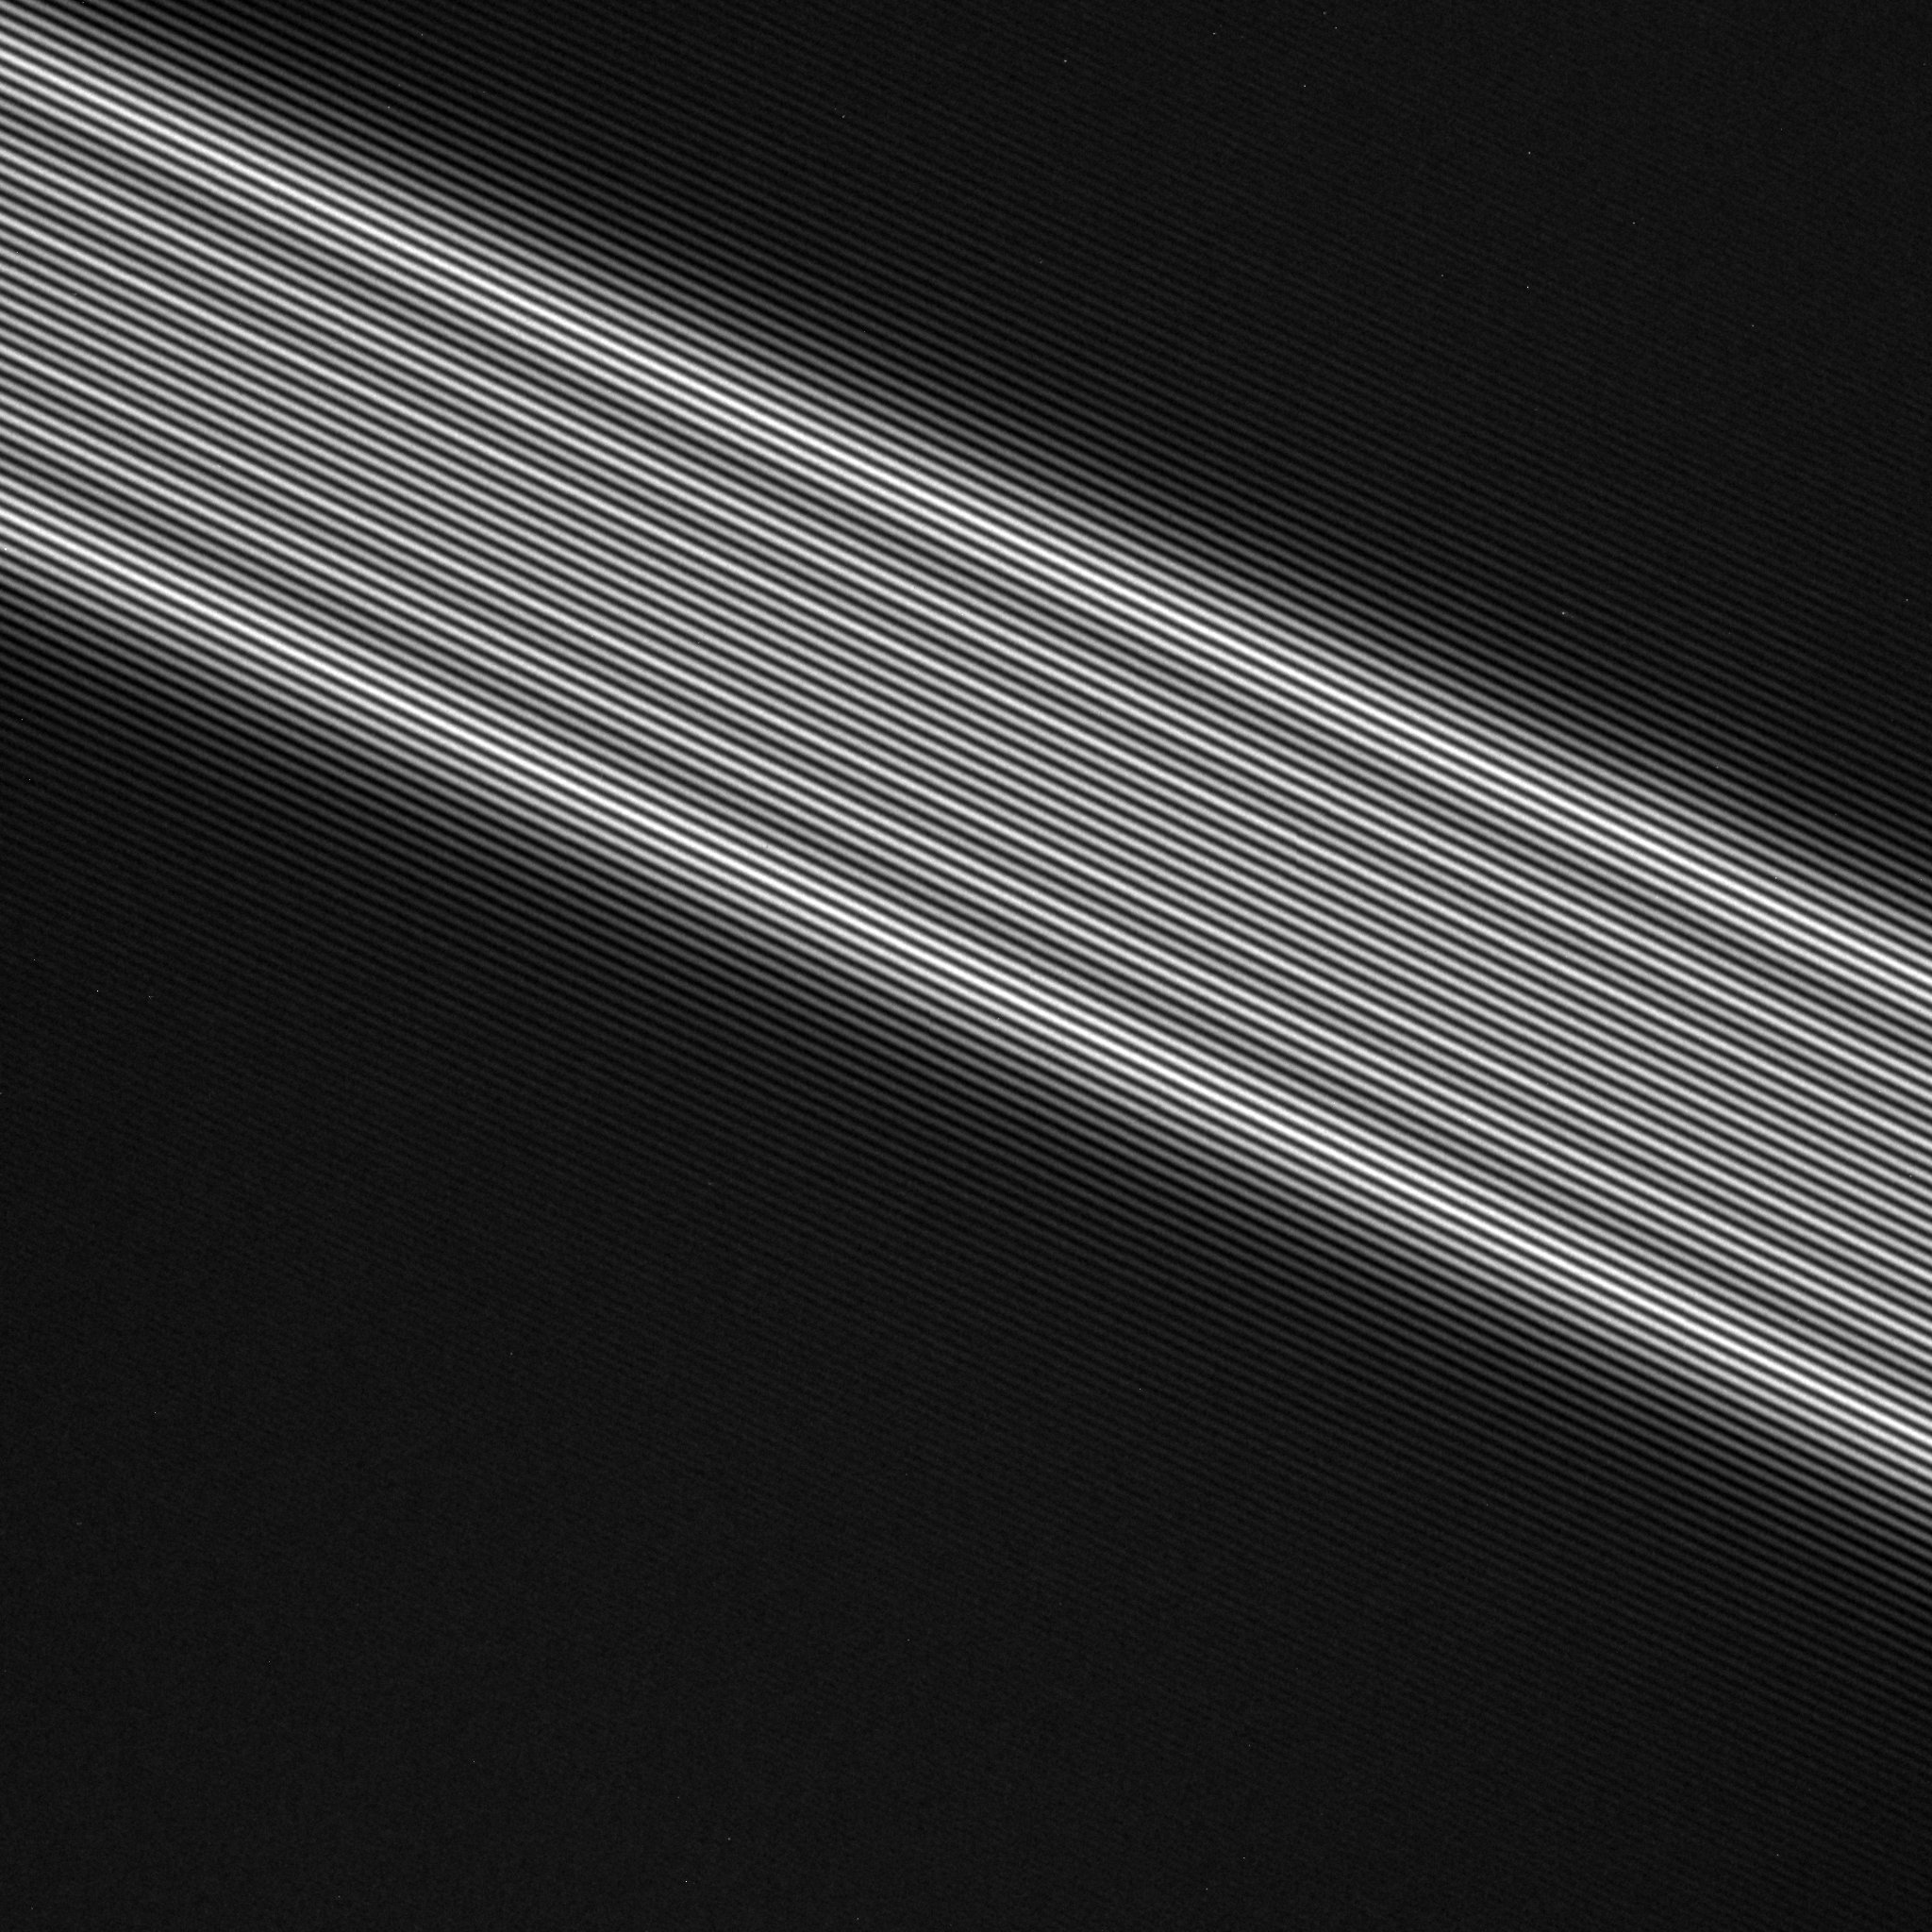
\includegraphics[width=\textwidth]{Holographie/Vakuumhologramm_Elliptischebeleuchtung/20_8_Vak_Ellip.jpg}
         \caption{\(U_F =\) 20,8V}
         \label{208VakEllip}
     \end{subfigure}
      
 %\vspace{}

 \centering
     \begin{subfigure}[b]{0.49\textwidth}
         \centering
         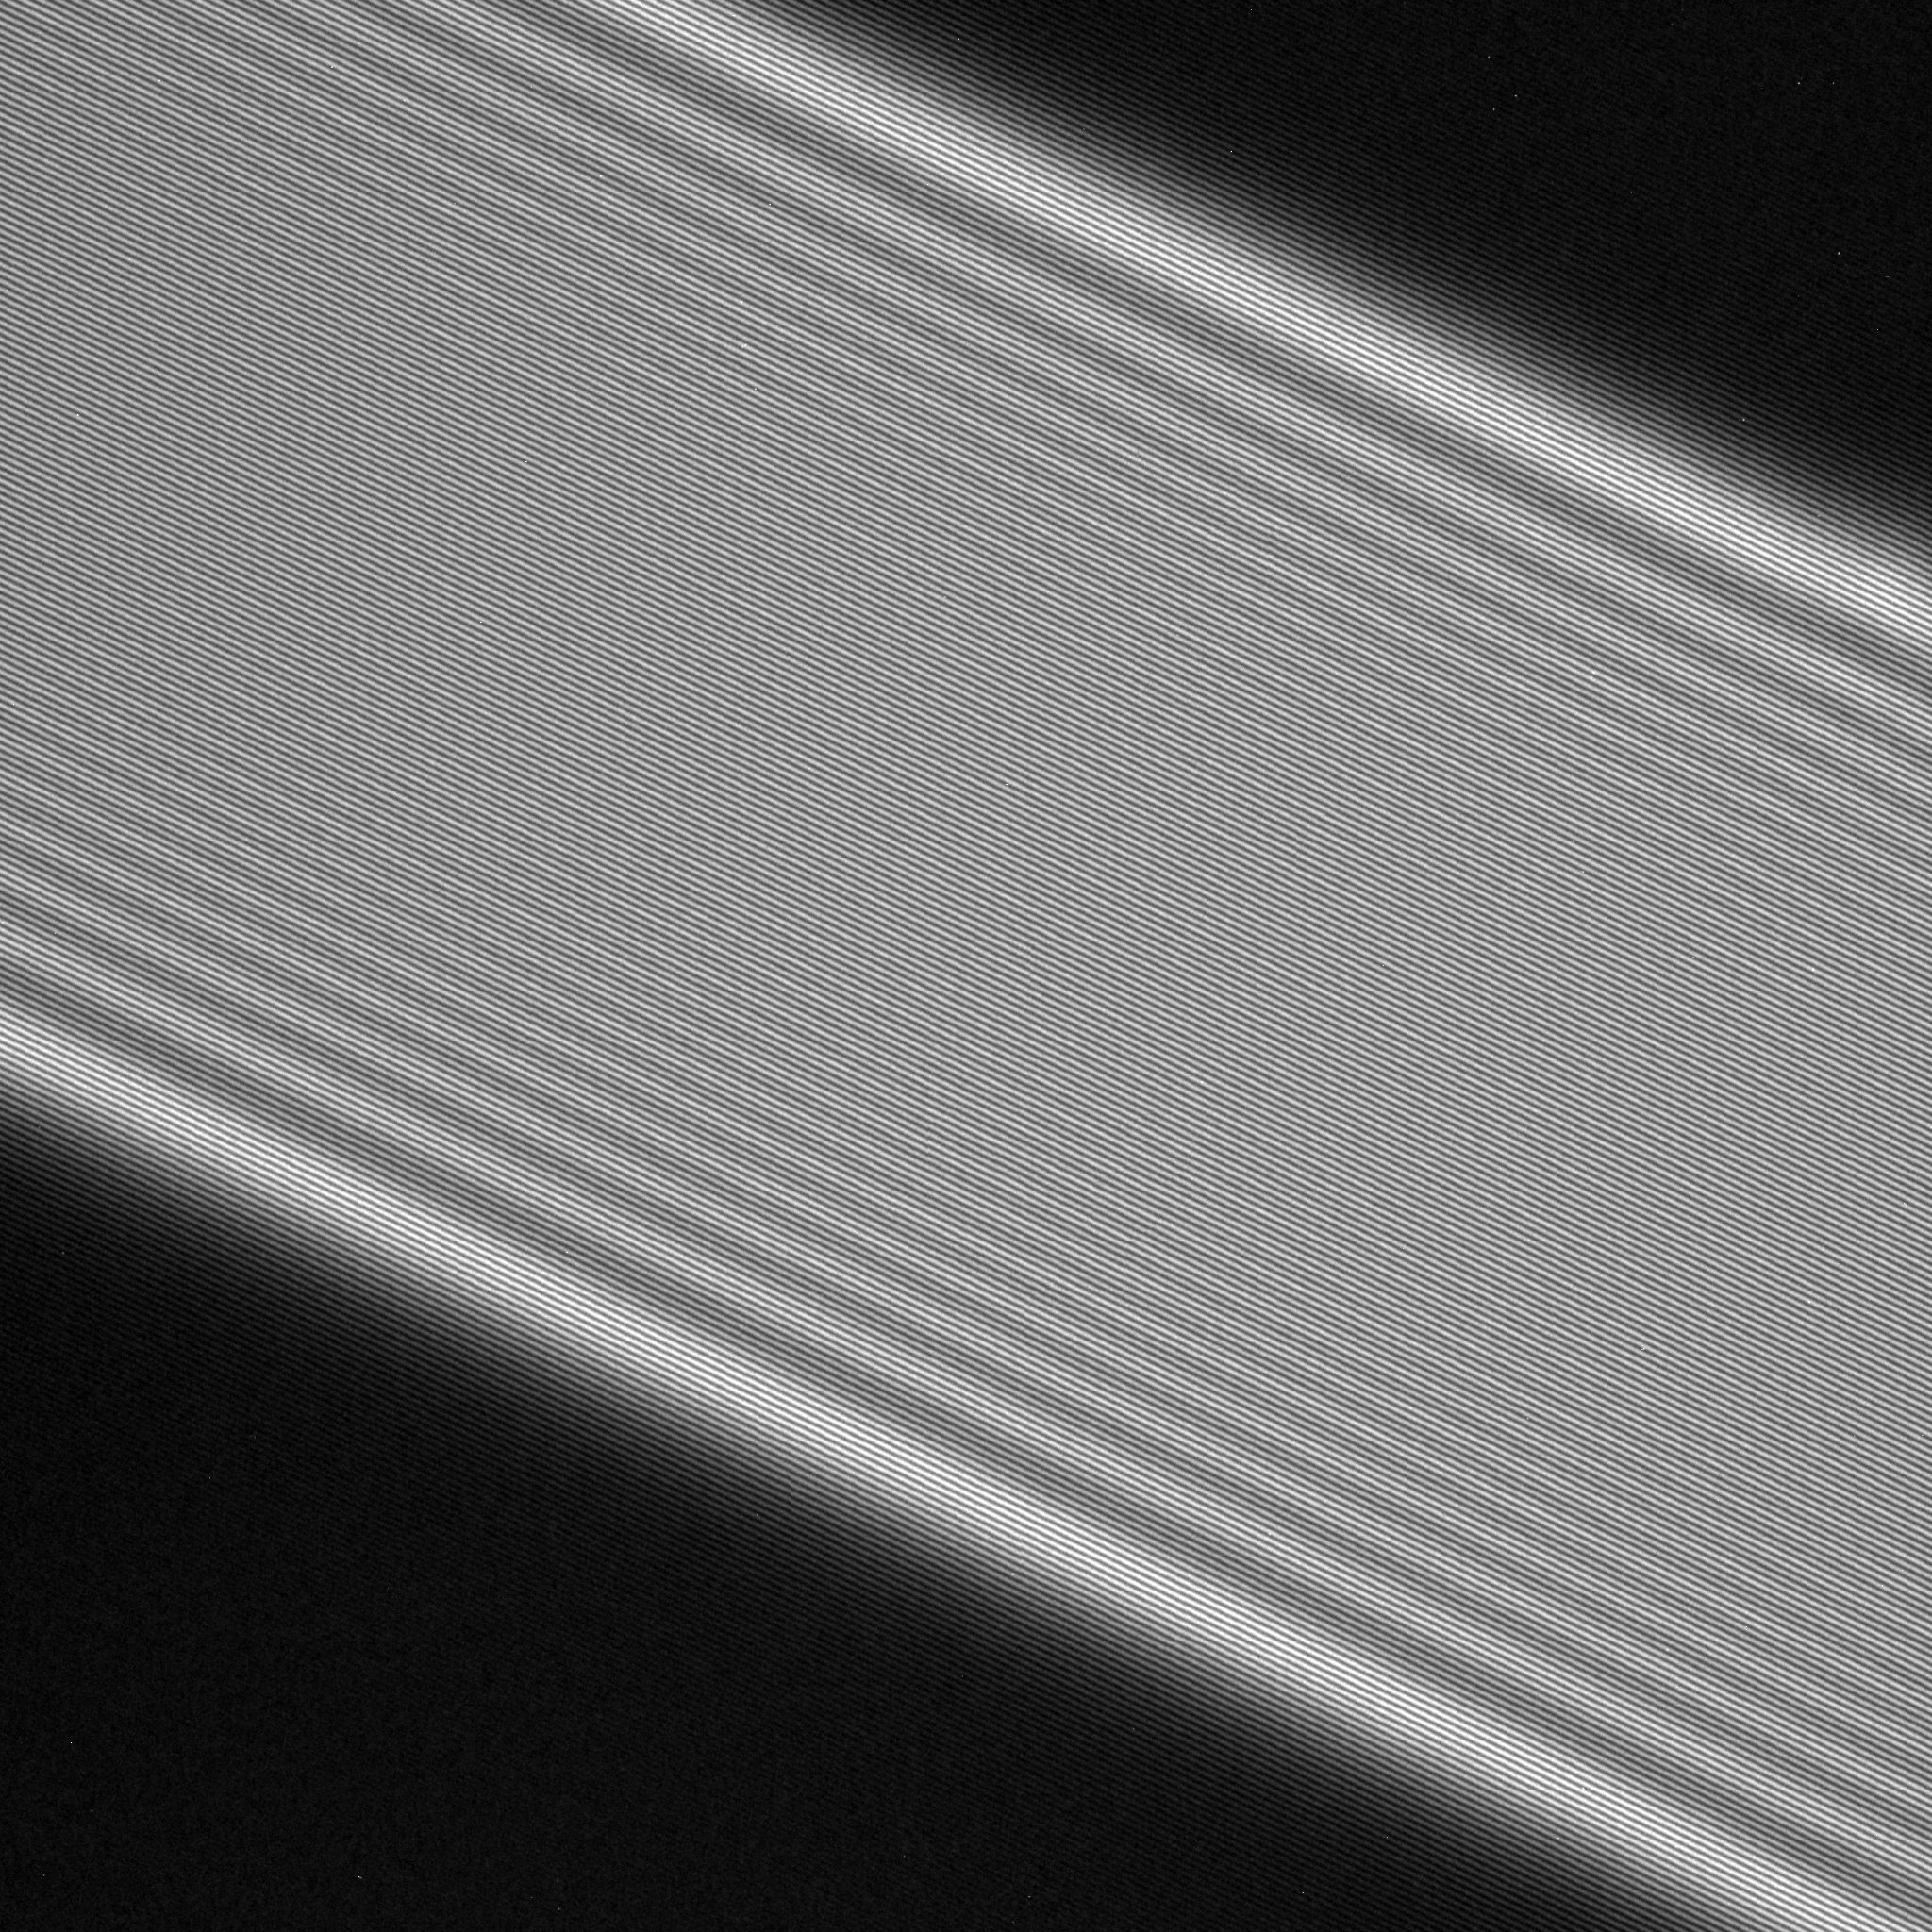
\includegraphics[width=\textwidth]{Holographie/Vakuumhologramm_Elliptischebeleuchtung/60_7_Vak_Ellip.jpg}
         \caption{\(U_F =\) 60,7V}
         \label{604VakEllip}
     \end{subfigure}
     \hfill
     \begin{subfigure}[b]{0.49\textwidth}
         \centering
         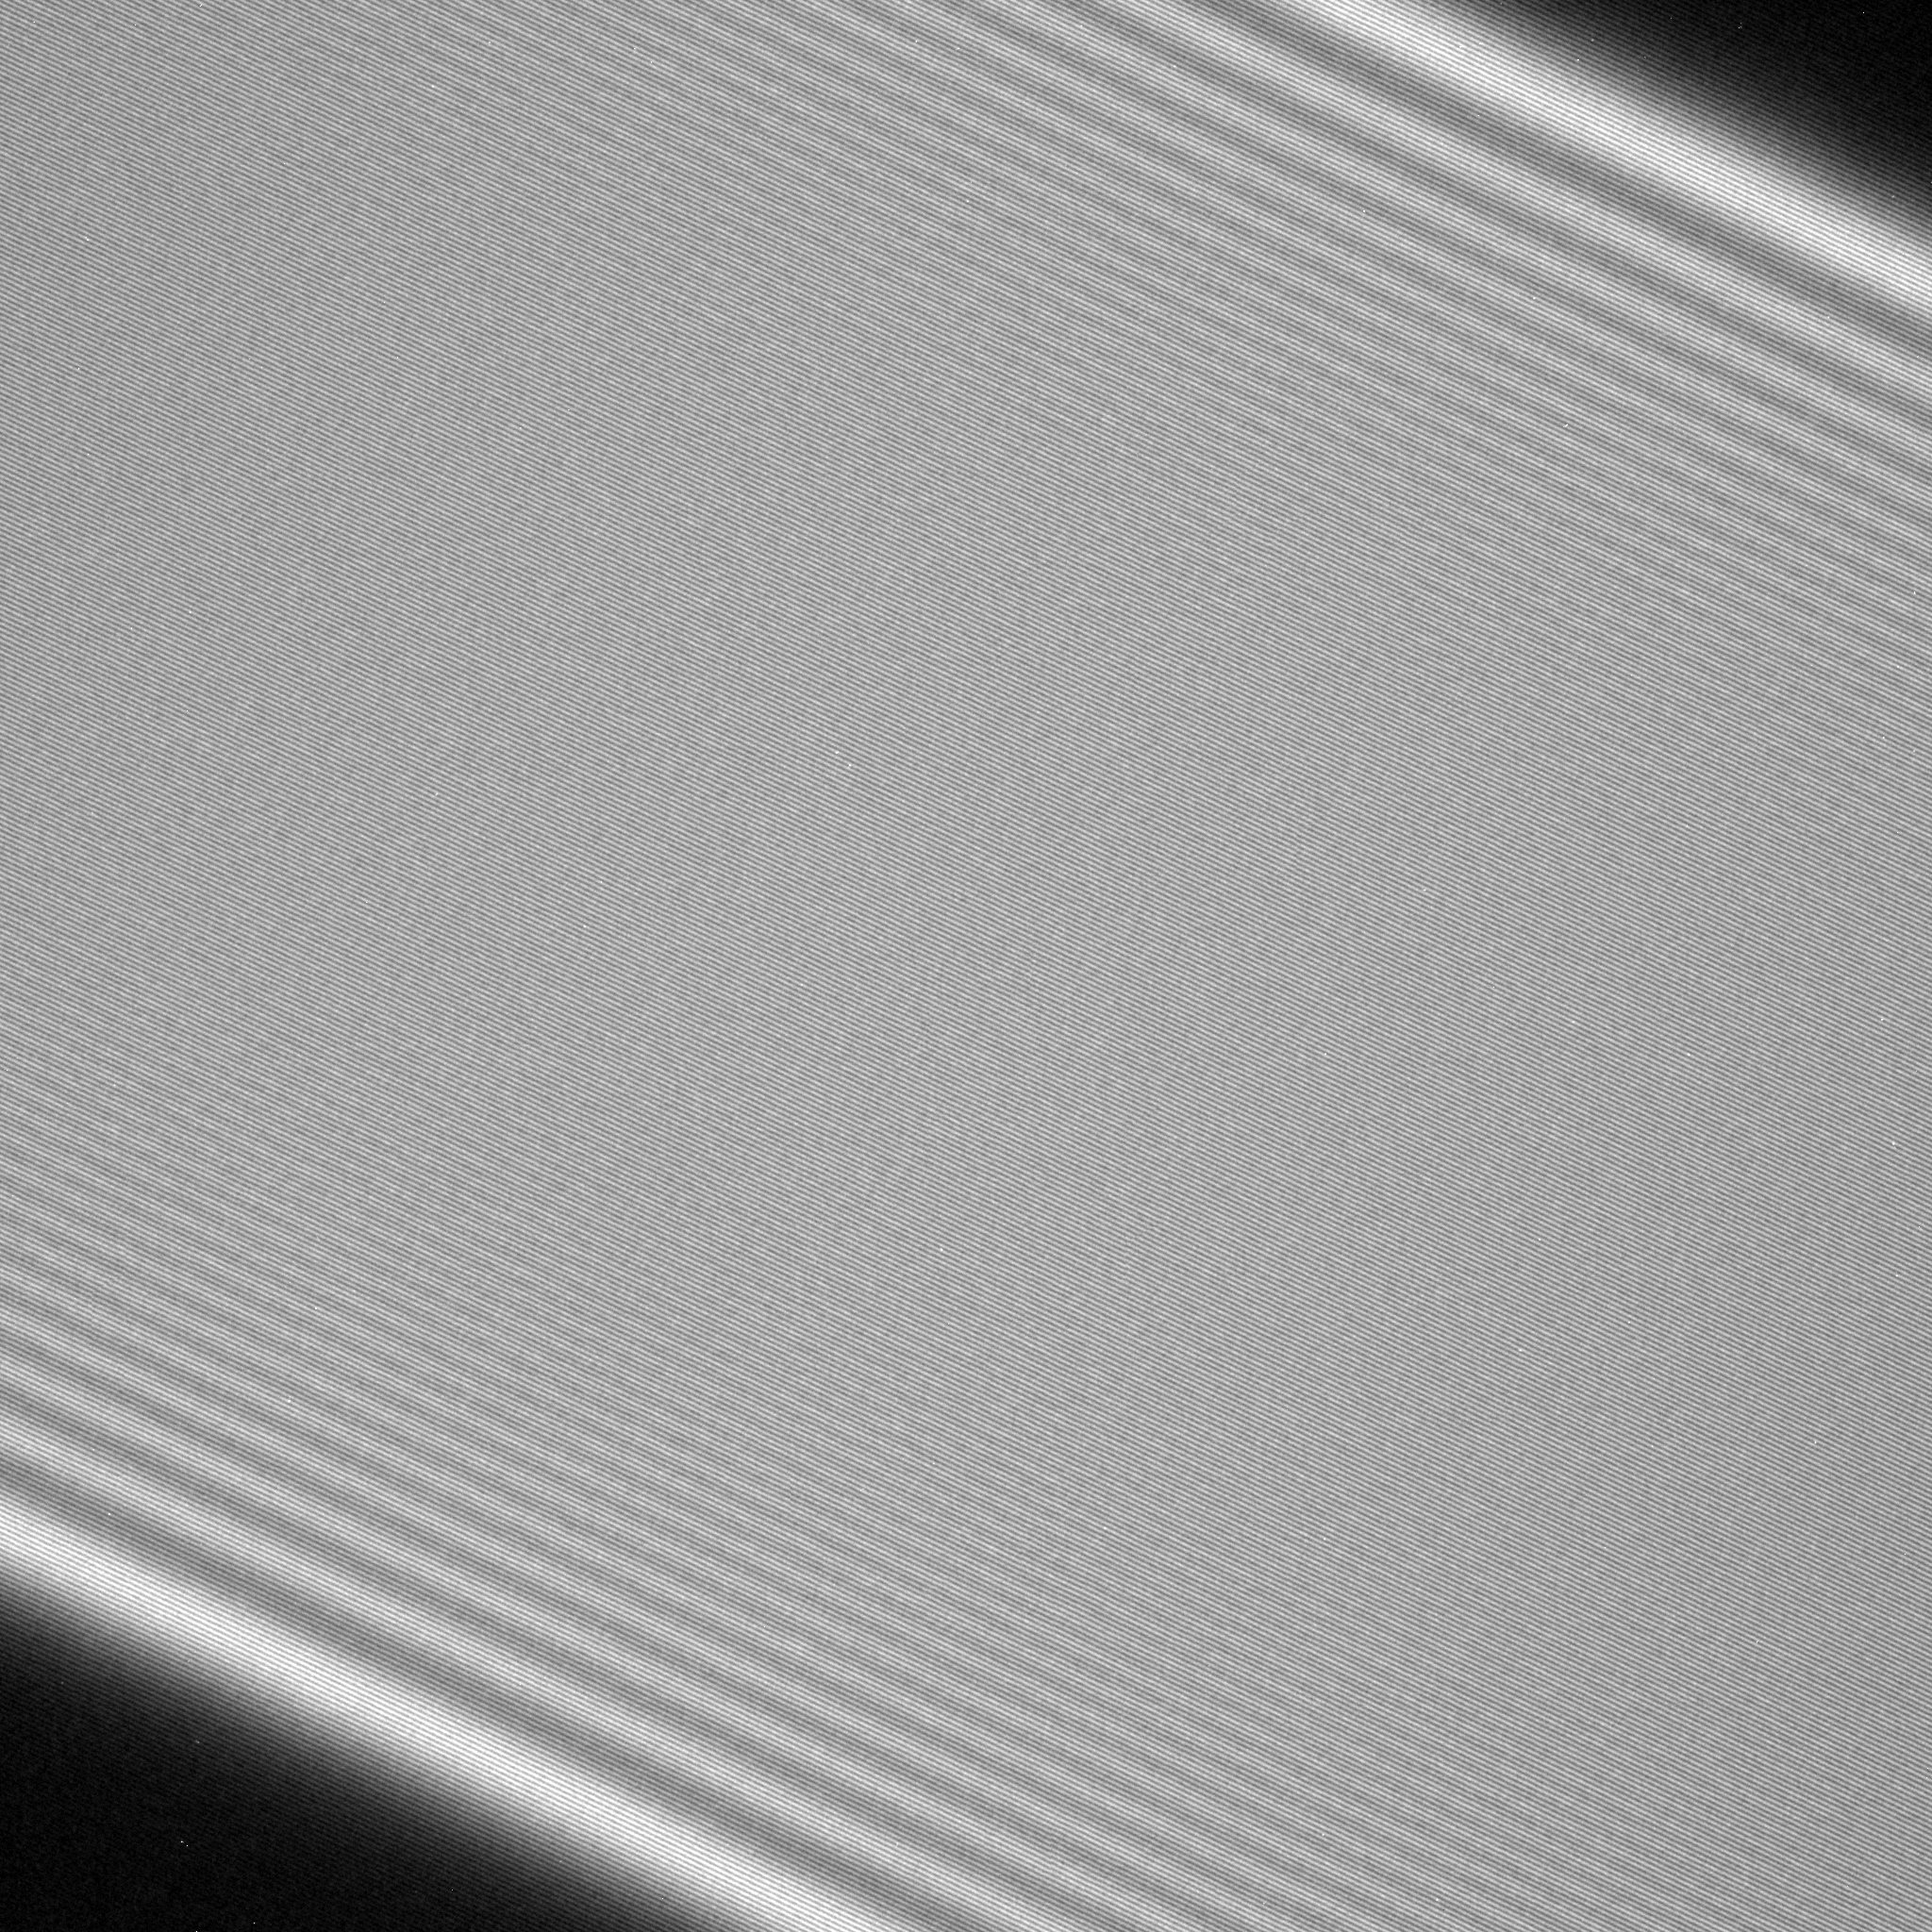
\includegraphics[width=\textwidth]{Holographie/Vakuumhologramm_Elliptischebeleuchtung/89_6_Vak_Ellip.jpg}
         \caption{\(U_F =\) 89,6V}
         \label{896VakEllip}
     \end{subfigure}
     \caption{Leerhologramm mit Elliptischen Beleuchtung bei verschiedenen Fadenspannungen}
        \label{VakHolEllip}
 
\end{figure}

\subsection{P-N Übergang}

Als nächstens wurde eine Silizium Probe untersucht, in der ein P-N Übergang untersucht werden sollte. Zunächst wurde die Probe eingesetzt und nachdem das Vakuum sich stabilisierst hatte wurde das Mikroskop neu eingestellt. Der Probenhalter wurde nun so verkippt das im TEM Modus die Biegekonturen so gering wie möglich erschienen und vor allem in den P-N Übergangsbereich nicht vorhanden waren. Eine Übersichtsaufnahme der Probe ist in Abbildung \cref{P-NÜbersicht} zu sehen, und zwei Aufnahme mit und ohne Biegekonturen im P-N Übergangsbereich sind in Abbildung \cref{P-NOhneKonturen} und \cref{P-NMitKonturen} zu sehn.

\begin{figure}
     \centering
     \begin{subfigure}[b]{0.3\textwidth}
         \centering
         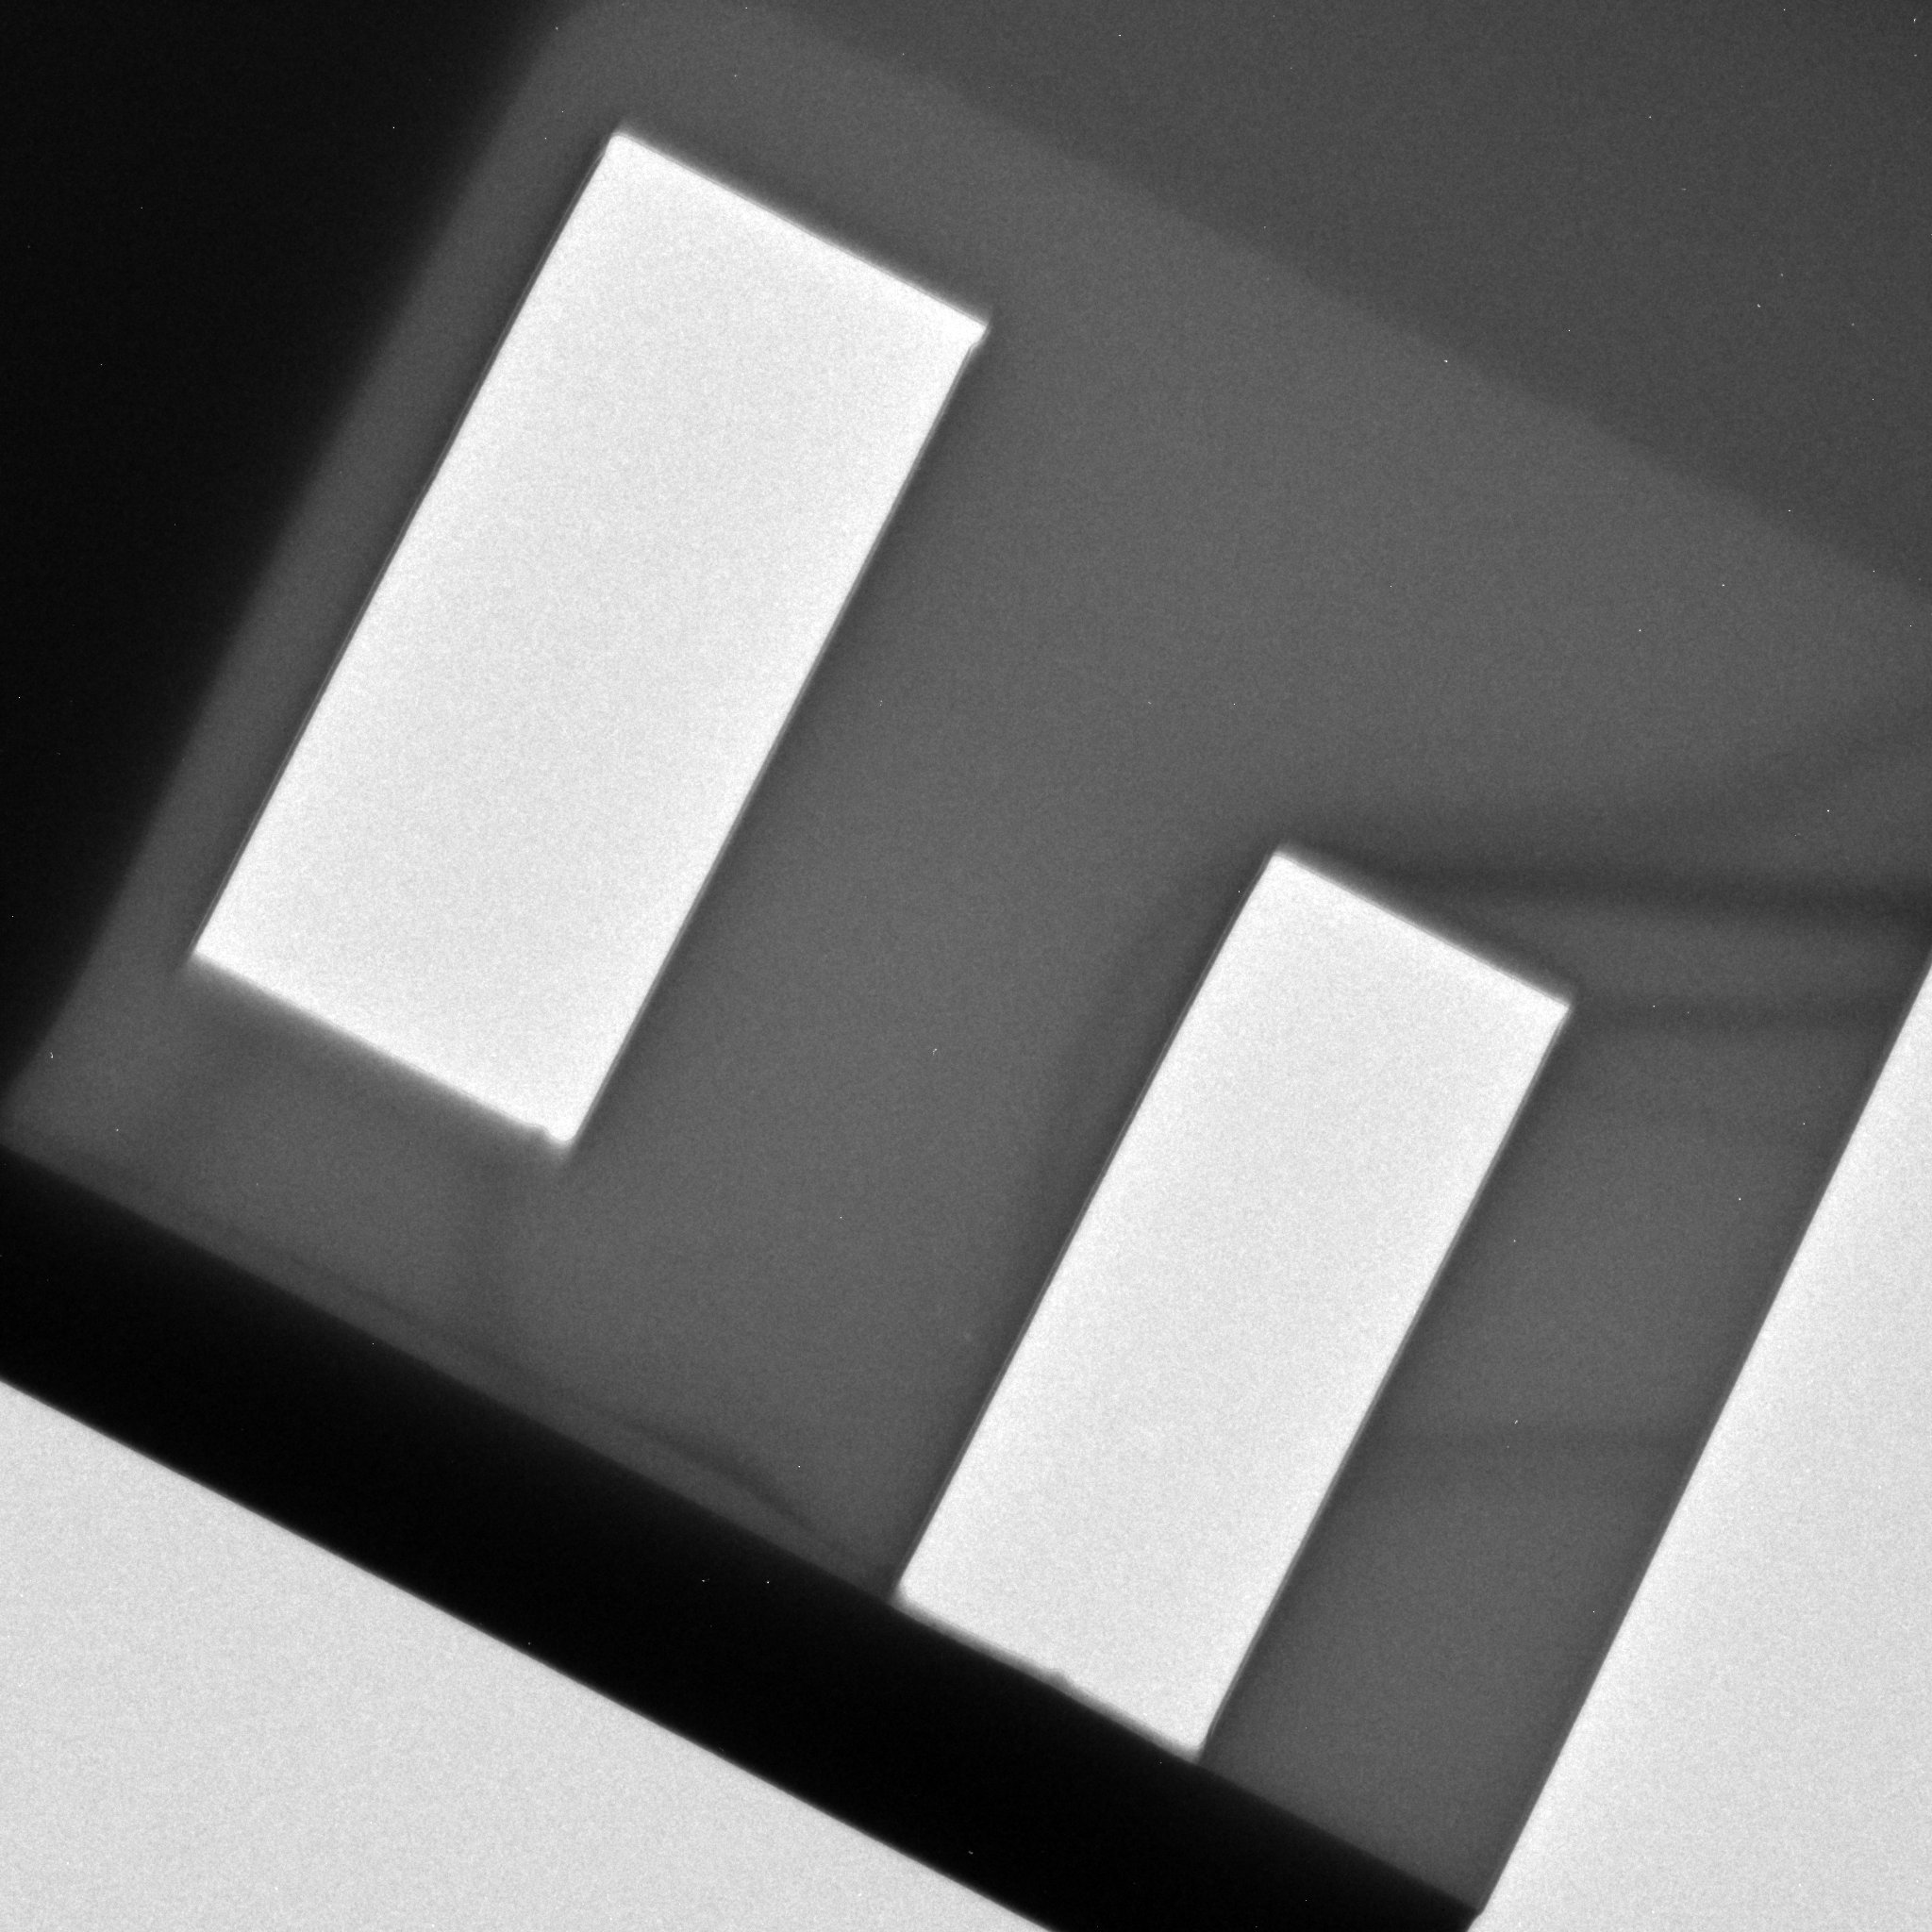
\includegraphics[width=\textwidth]{Holographie/Probe/1_Übersicht1750x_LTZ.jpg}
         \caption{Ganze Probe}
         \label{P-NÜbersicht}
     \end{subfigure}
     \hfill
     \begin{subfigure}[b]{0.3\textwidth}
         \centering
         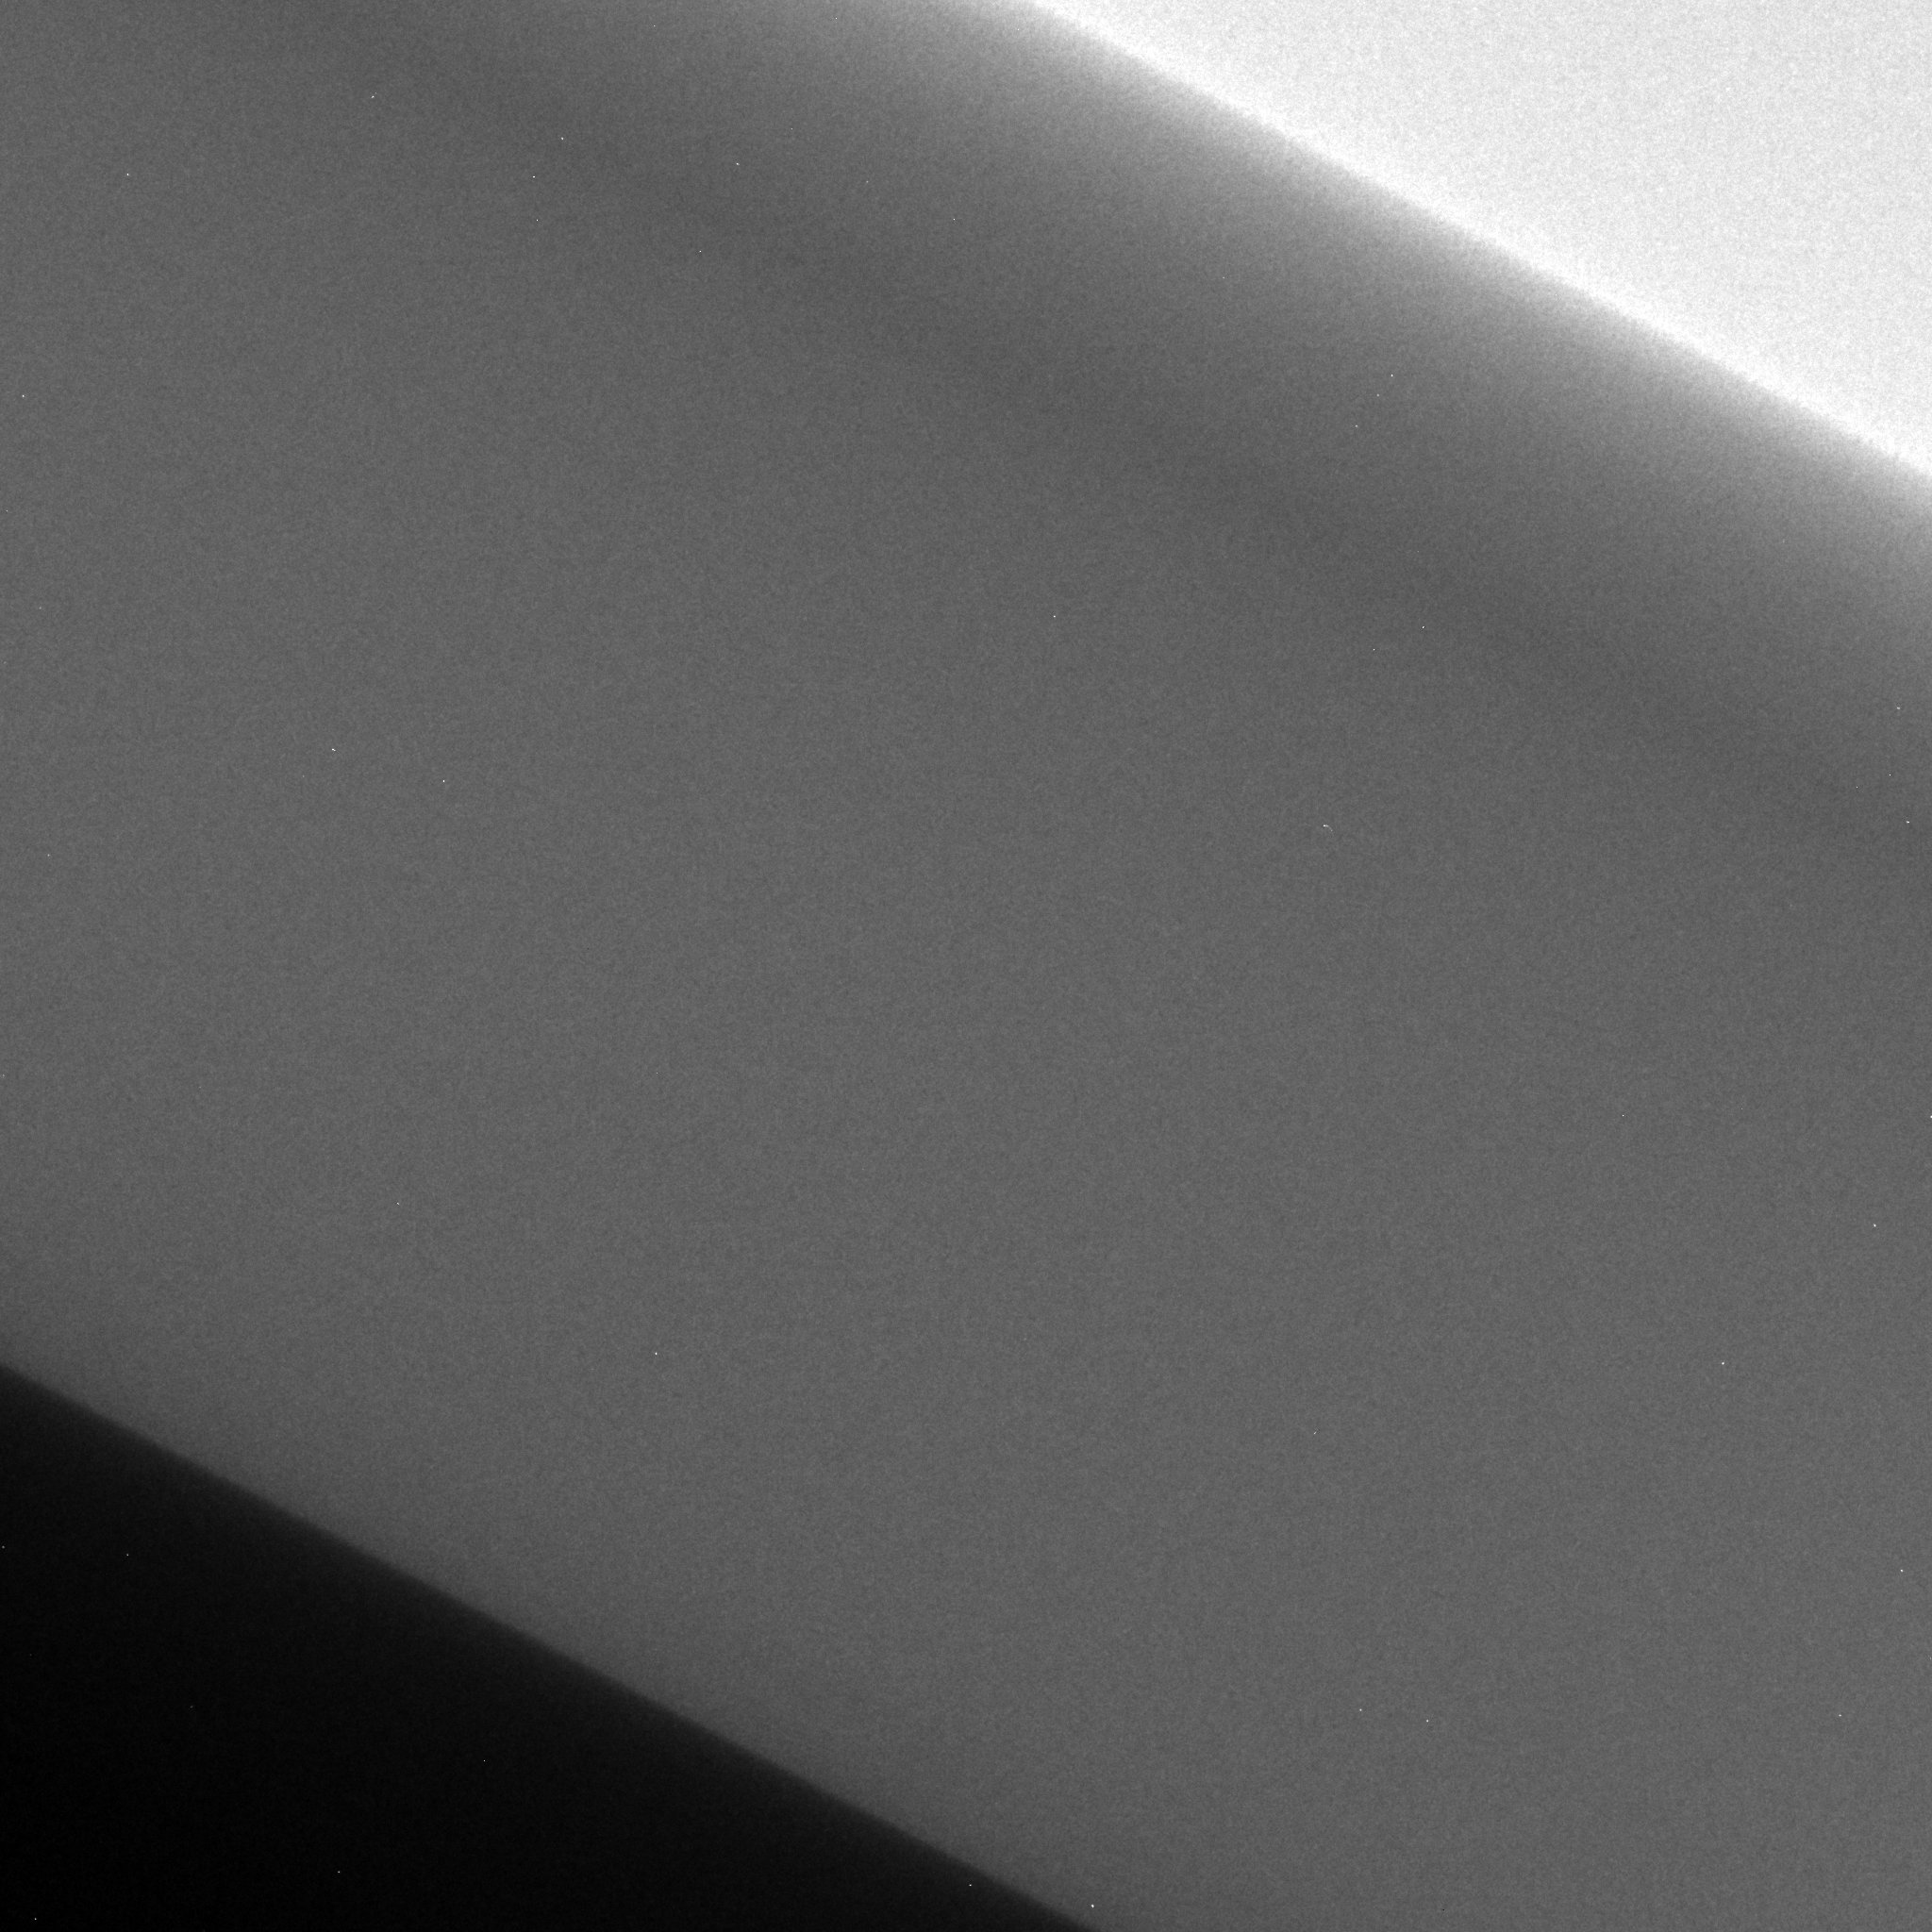
\includegraphics[width=\textwidth]{Holographie/Probe/3_OhneBiegekonuren13500x_LTZ.jpg}
         \caption{P-N Übergang, ohne Biegekonturen.}
         \label{P-NOhneKonturen}
     \end{subfigure}
     \hfill
     \begin{subfigure}[b]{0.3\textwidth}
         \centering
         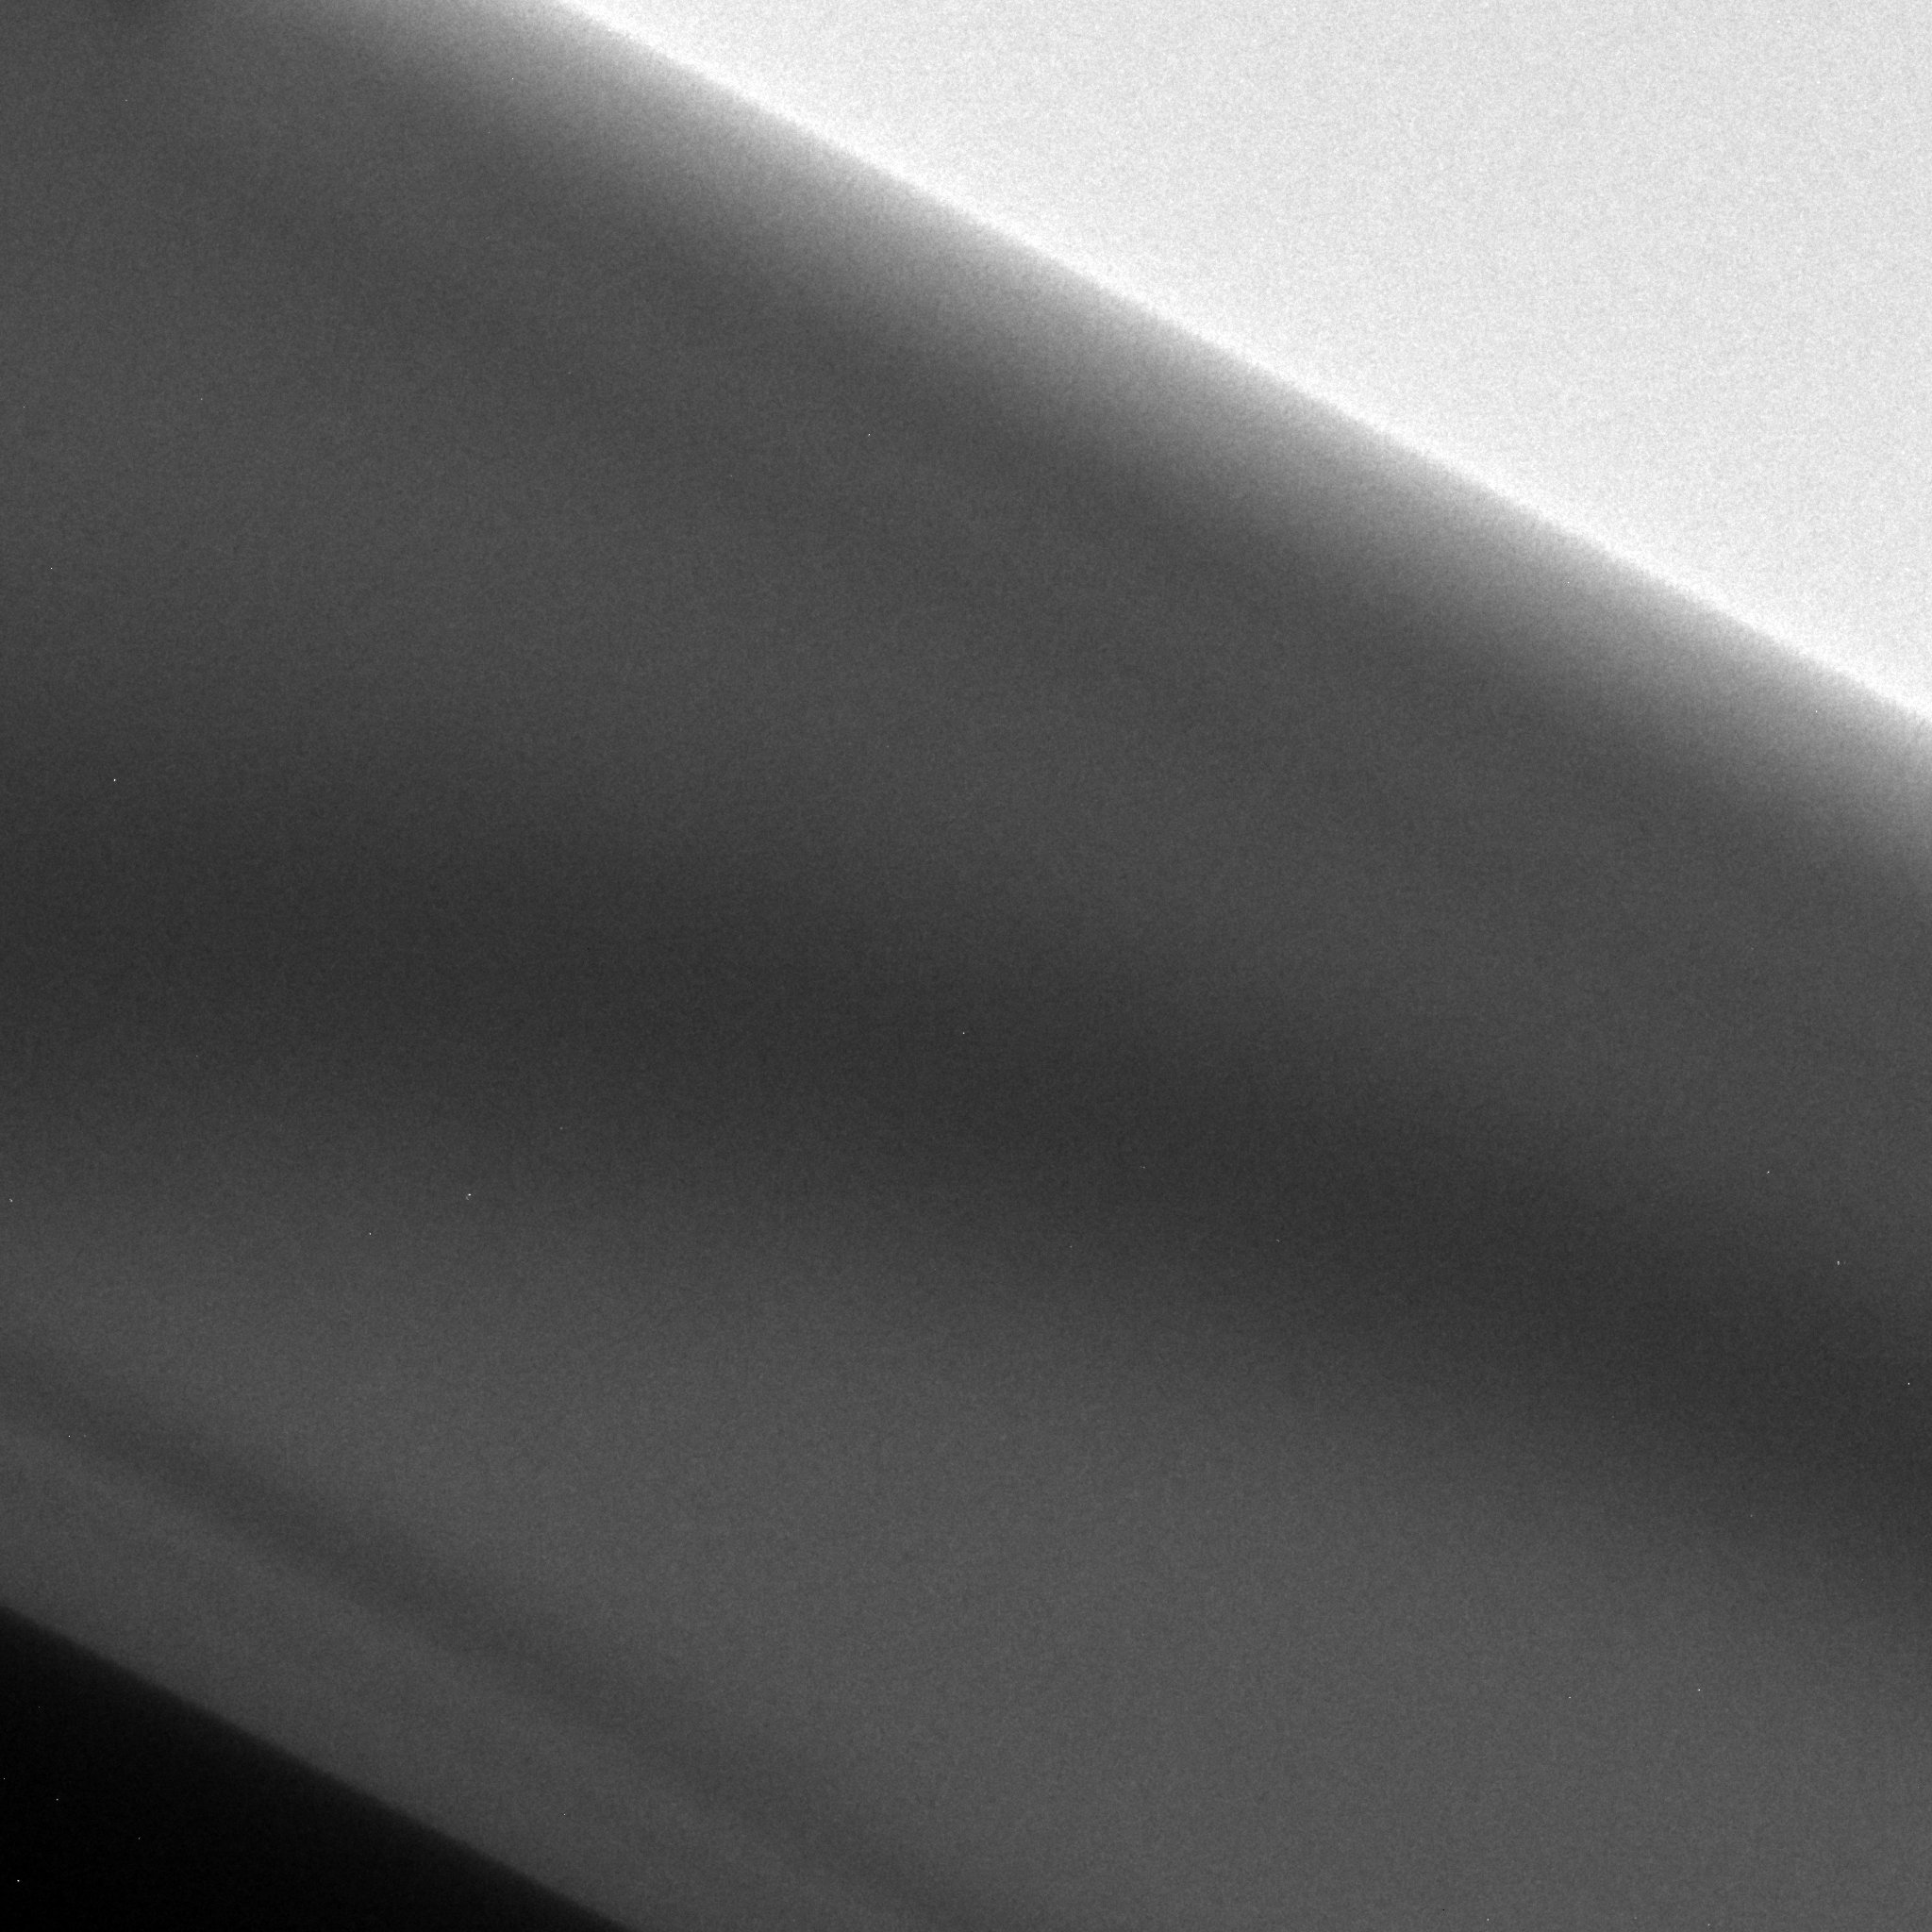
\includegraphics[width=\textwidth]{Holographie/Probe/2_Biegekontur13500x_LTZ.jpg}
         \caption{P-N Übergang, mit Biegekonturen.}
         \label{P-NMitKonturen}
     \end{subfigure}
        \caption{Übersichtsaufnahme der Ganzen Probe (a), und des P-N Übergang (b), (c) mit und ohne Biegekonturen}
        \label{P-NTEMÜbersicht}
\end{figure}

Die Probe wurde so verfahren das das durch die Fokussierte Ionen Dünnung (FIB) erstellte Vakuum Fenster in der Probe so positioniert war das ein Leerhologramm durch das Fenster erstellt werden konnte. Dabei wurde eine Rundbeleuchtung verwendet und eine Fadenspannung von 70V. Abbildung \cref{P-NLeer}\\
Anschließen wurde die Probe so verfahren das sich der Biprisma Faden an der Kante des festeres befand, um nun zwei gut separate Teilwellen für das Hologramm erhalten zu können. Hier wurde eine Hologramm Aufnahme erstelle, bei der die Mikroskope Einstellungen des Leer Hologramm beibehalten wurden. Das Hologramm ist in Abbildung \cref{P-NObjekt} zu sehen.\\
Die Messungen wurden analog zur rund Beleuchtung mit einer elliptischen Beleuchtung wiederholt.

\begin{figure}[H]
     \centering
     \begin{subfigure}[b]{0.49\textwidth}
         \centering
         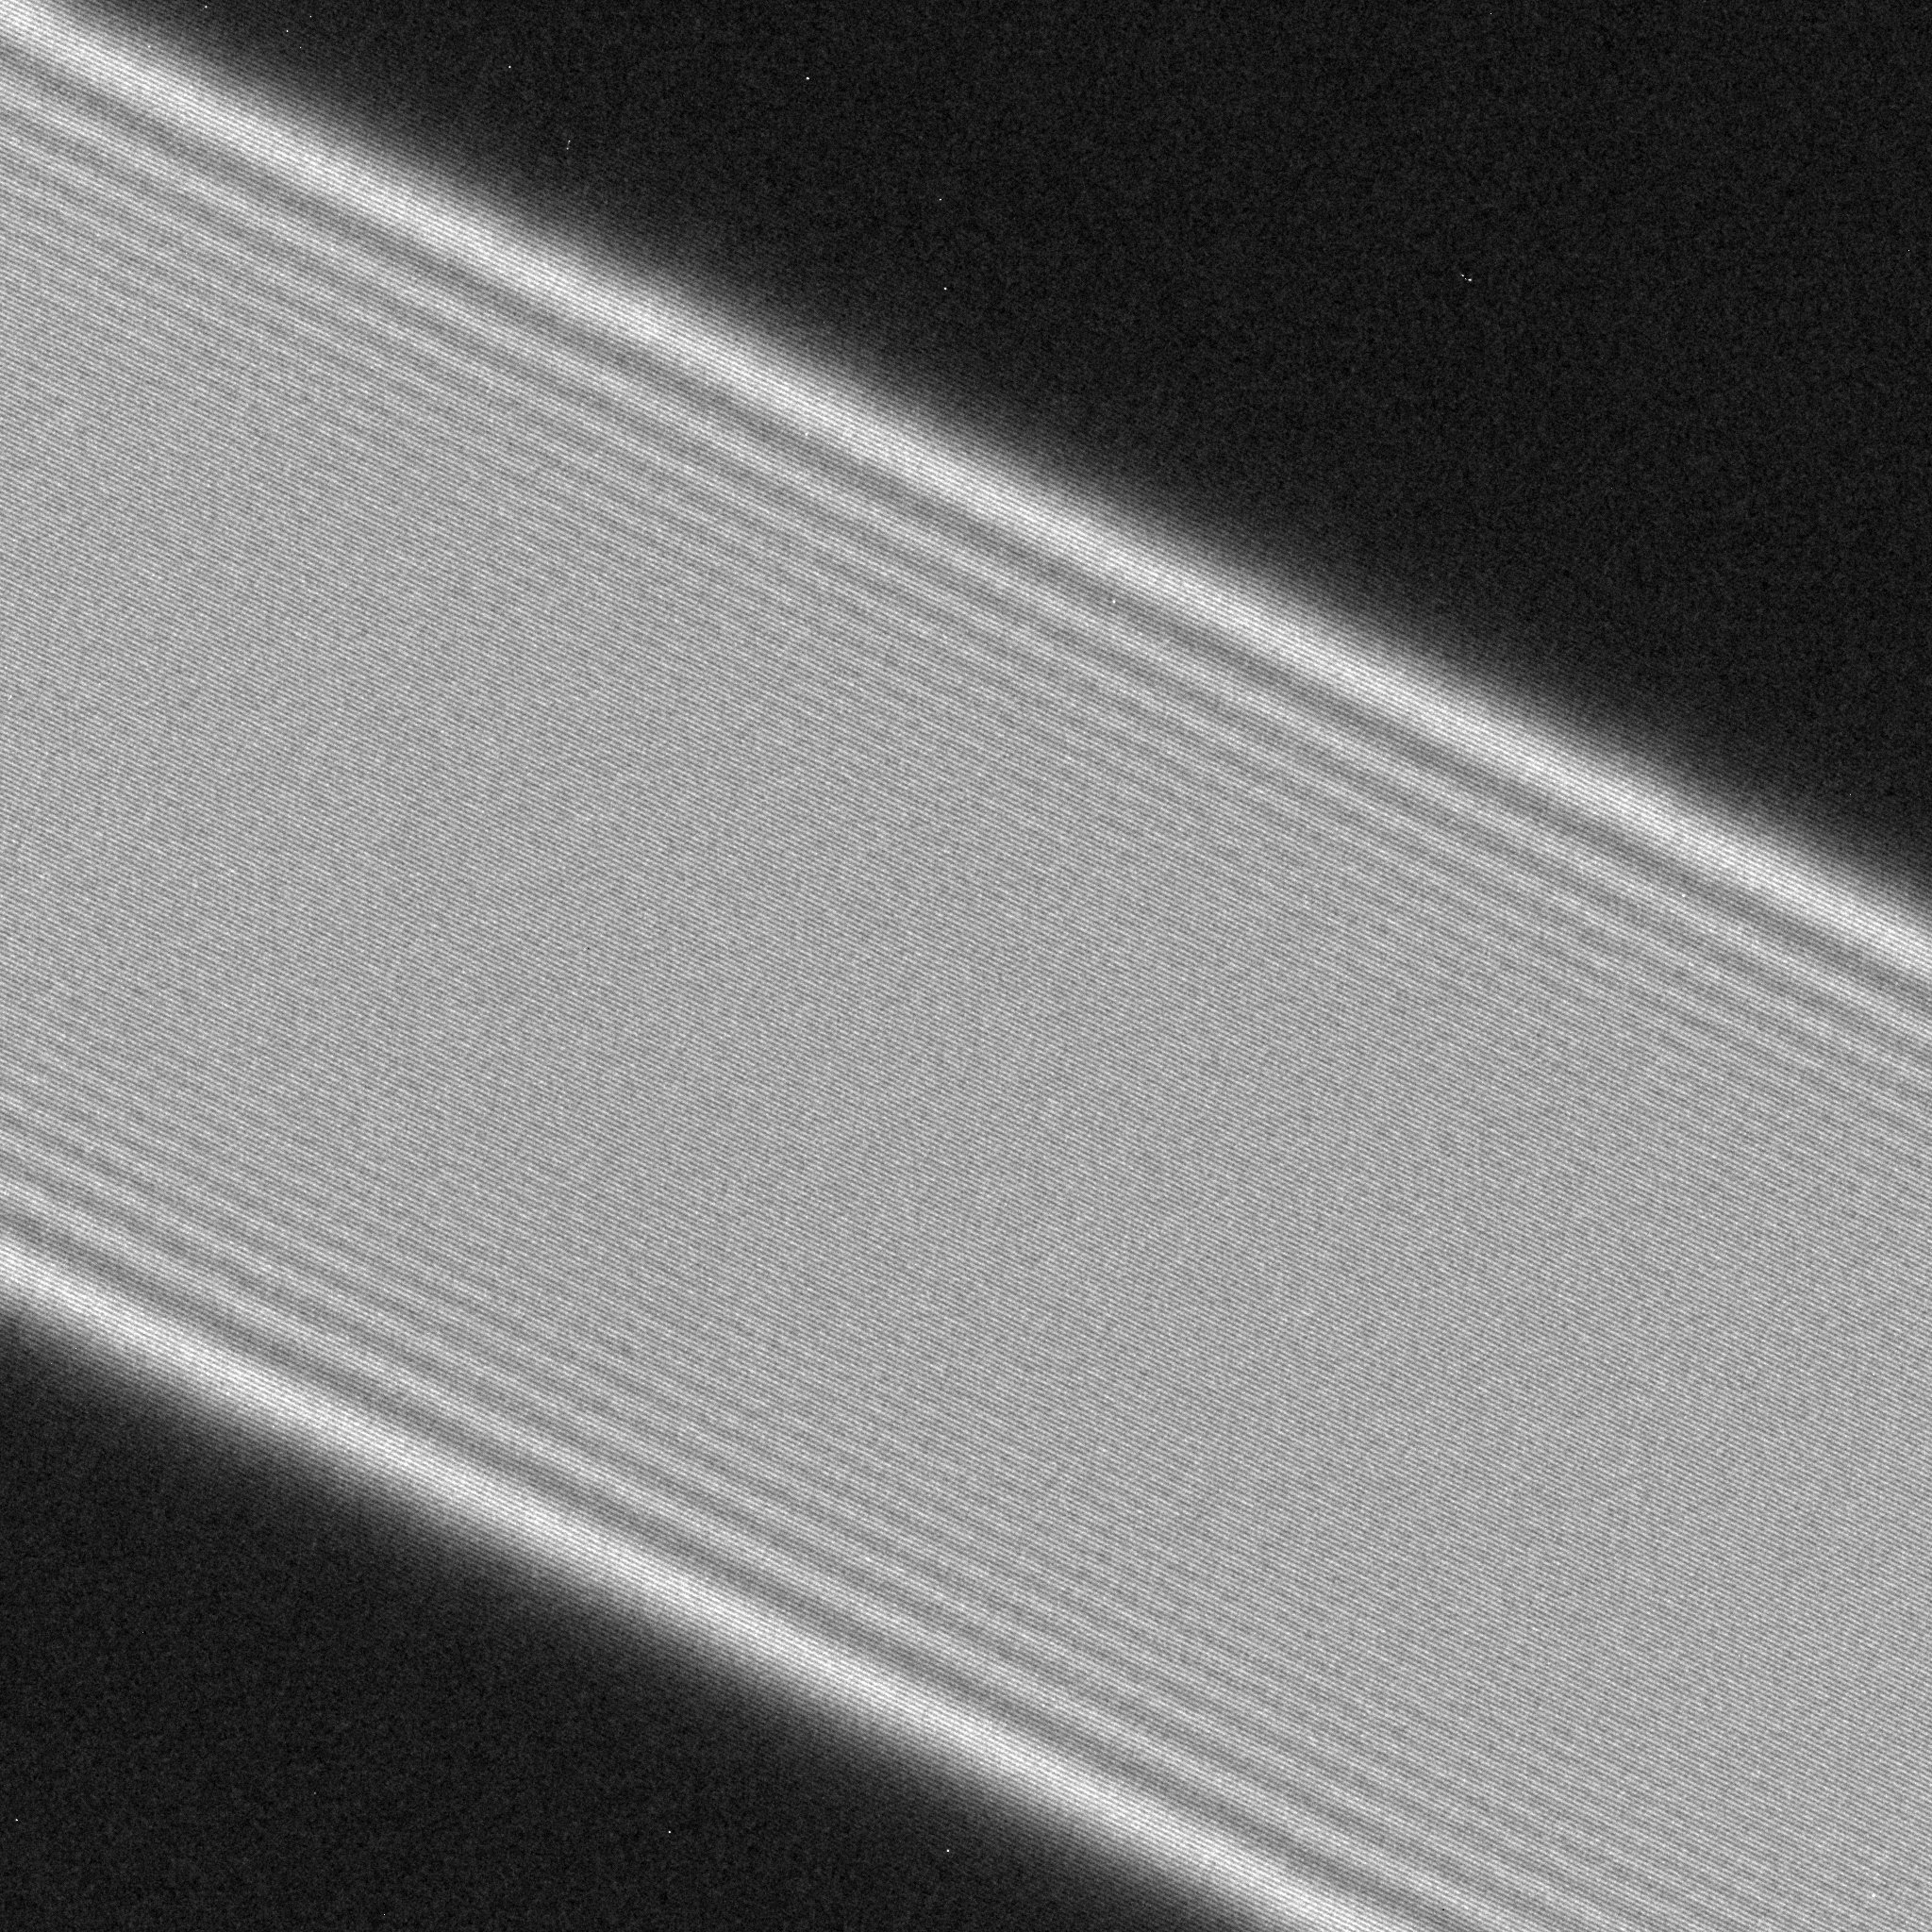
\includegraphics[width=\textwidth]{Gerüst/Abbildungen/Holographie/Probe/4_Rundbeleuchtung_Hologram_15500x_LTZ.jpg}
         \caption{Leerhologramm}
         \label{P-NLeer}
     \end{subfigure}
     \hfill
     \begin{subfigure}[b]{0.49\textwidth}
         \centering
         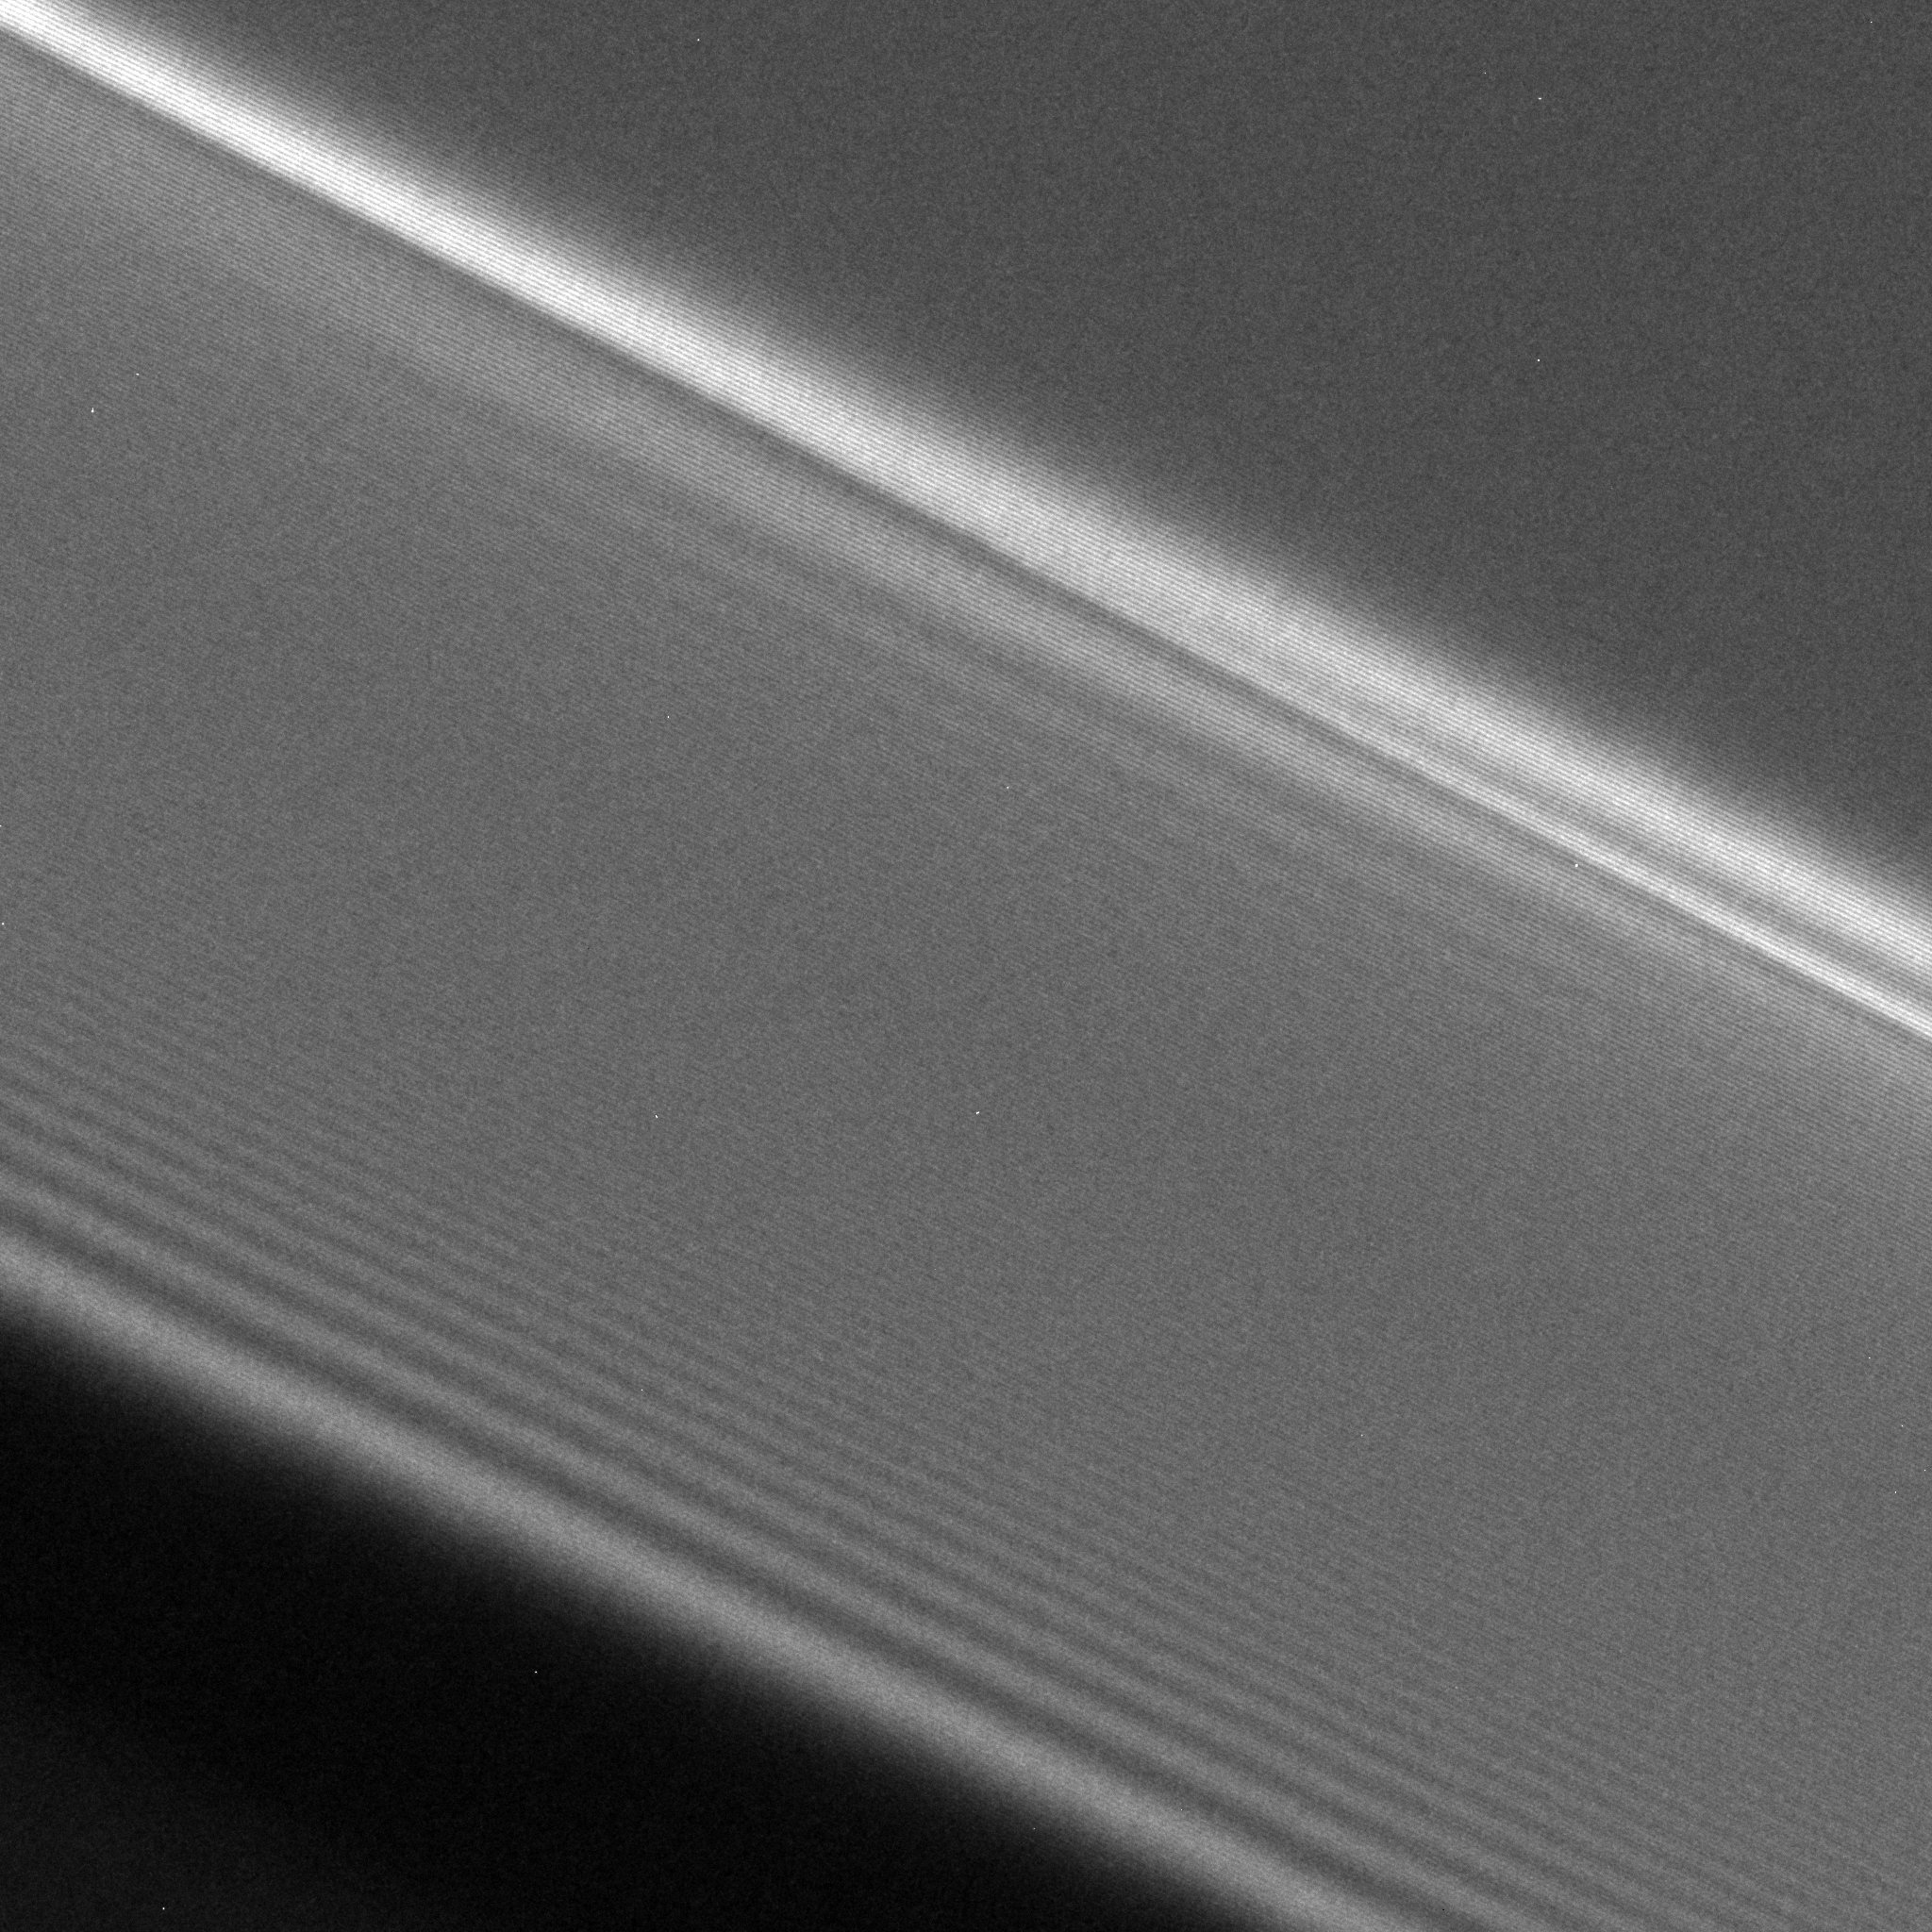
\includegraphics[width=\textwidth]{Gerüst/Abbildungen/Holographie/Probe/5_Rundbeleuchtung_Hologram_an_derKante_15500x_LTZ.jpg}
         \caption{Objekthologramm}
         \label{P-NObjekt}
     \end{subfigure}
        \caption{Hologramm Aufnahme von Silizum Chip mit P-N Übergang}
        \label{AmpPhaseBild}
\end{figure}

\subsubsection{Rekonstruktion des Hologramms}

Um aus dem Hologramm die Phasen und Amplitudeninformation zu erhalten, muss man die komplexe bildwelle rekonstruieren. Hierfür wird zunächst eine Fast Fourier Transformation aus dem Hologramm erstellt. Dabei entsteht eine Komplexes Fourier Spektrum. In diesem Fourier Spektrum ist das Zentralband mit zwei Seiten Bänder (Seitenband -1 und Seitenband +1) abgebildet.\\
Zur Rekonstruktion wird das Seitenband +1 verwendet, dies ist das das Vakuum seitige band. Dieses Band wird ausgeschnitten und zentriert um es anschließend Inverse Fourier zu transformieren. Dadurch wird die Komplexe Bildwelle erstellt.

\subsubsection{Leerhologramm und Korrektur}

Um die Qualität der Bildwelle zu verbessern kann ein Leerhologramm verwendet werden, dadurch kann die verzeichnungsbedingte Phasenmodulation korrigieren werden. Die Korrektur wird erreicht, wenn die bei der Rekonstruktion erhaltene Bildwelle durch die Vakuum Bildwelle geteilt wird. Dabei werden die Amplituden miteinander geteilt und die Phasen voneinander abgezogen. Als Resultat erhält man nun ein korrigiertes Phasen und Amplitudenbild.

\subsubsection{Auswertung}

Im Amplitudenbild mit der rund Beleuchtung Abbildung \cref{P-NAmp} ist der P-N Übergang nicht erkennbar es ist lediglich die Kante zum Vakuum (Oben Rechts) erkennbar. \\
Beim dem Phasenbild ist der P-N Übergang wesentlich besser zu erkenn, siehe Abbildung \cref{P-NPhaseW} (Wrappt), es ist hier ein klarer Kontrast erkennbar der etwas unter der Kante zum Vakuum liegt. Sowie bei dem durch dem Goldsted Algorithmus Bearbeitetem (Unwraped) Phasenbild \cref{P-NphaseU}. 

\begin{figure}
     \centering
     \begin{subfigure}[b]{0.3\textwidth}
         \centering
         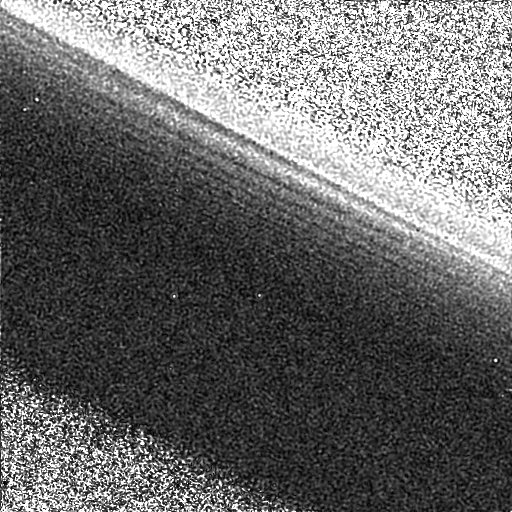
\includegraphics[width=\textwidth]{Holographie/Probe/6_Rundbeleuchtung_amplitude_keil.jpg}
         \caption{Amplitudenbild}
         \label{P-NAmp}
     \end{subfigure}
     \hfill
     \begin{subfigure}[b]{0.3\textwidth}
         \centering
         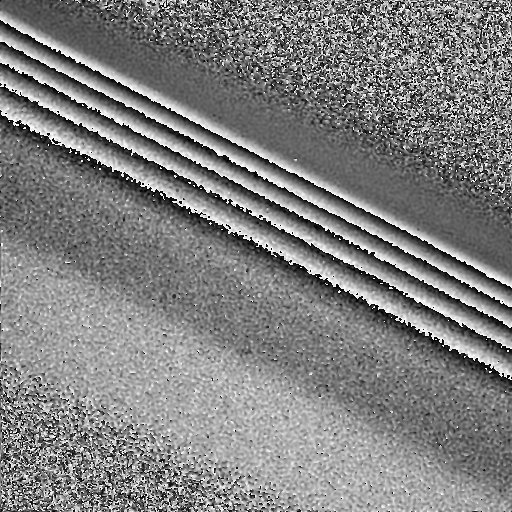
\includegraphics[width=\textwidth]{Holographie/Probe/7_Rundbeleuchtung_Unkorigirten_Phase_über_ort_15500x_LTZ.jpg}
         \caption{Phasenbild, Wrapped}
         \label{P-NPhaseW}
     \end{subfigure}
     \hfill
     \begin{subfigure}[b]{0.3\textwidth}
         \centering
         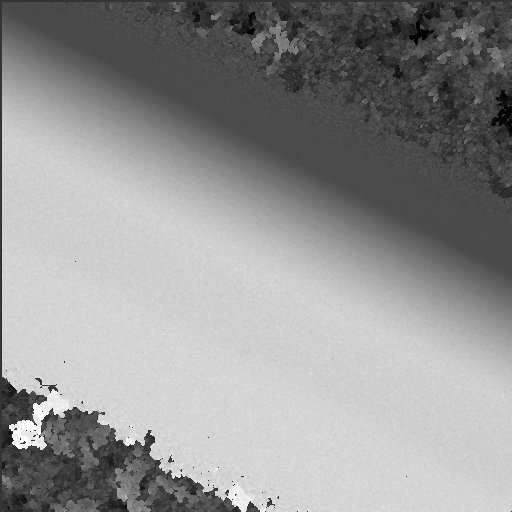
\includegraphics[width=\textwidth]{Holographie/Probe/8_Rundbeleuchtung_Korrigiert_Unwraptbild_15500x_LTZ.jpg}
         \caption{Phasenbild, Unwrapped}
         \label{P-NphaseU}
     \end{subfigure}
        \caption{}
        \label{P-NTEMÜber}
\end{figure}

Die Unwrapped Phasenkeil Aufnahme kann verwendet werden um die Dicke der Probe zu bestimmen dabei wird die Phasen Schiebung im Phasenkeil im Grapf \cref{P-NKeil} ausgewertet. Dabei kann abgelesen werden das die Phasenschiebung im Keil \(30 rad\) beträgt, wenn nun die Funktion \cref{eq:PhaseShift} zur Hilfe genommen wird kann die Dicke der Probe bestimmt werden. Hierbei wird das mittleres inneres potential, \(V^{Si}_{MIP} = 12.57V\) verwendet, um eine Objektdicke von \(350nm\) zu berechnet.

\begin{figure}[H]
     \centering
     \begin{subfigure}[b]{0.49\textwidth}
         \centering
         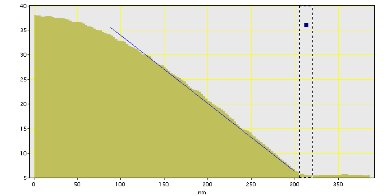
\includegraphics[width=\textwidth]{Gerüst/Abbildungen/Holographie/Probe/8_Rundbeleuchtung_Lieniendiagram_keil.jpg}
         \caption{Phasenkeil}
         \label{P-NKeil}
     \end{subfigure}
     \hfill
     \begin{subfigure}[b]{0.49\textwidth}
         \centering
         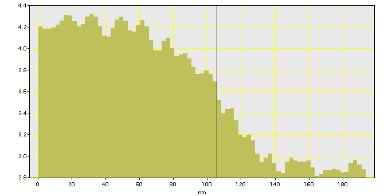
\includegraphics[width=\textwidth]{Gerüst/Abbildungen/Holographie/Probe/8_Rundbeleuchtung_Lieniendiagram_PN_übergang.jpg}
         \caption{P-N Übergang}
         \label{P-NPhase}
     \end{subfigure}
        \caption{Graph der Phasenschiebung des phasenkeil im Unwarapped Phasenbild (quer über den Keil gemessen) und des P-N Übergang um Wrapped Phasenbild (quer über den Übergang gemessen)}
        \label{P-NDiagram}
\end{figure}

In der unkorrigierten (Wrapped) Aufnahme ist ein Kontrast des P-N Übergang erkennbar, dieser entspricht der Phasenschiebung der durch das unterschiedlichen Elektrische Potential im P-N Übergang verursacht wird. Die Phasenschiebung im P-N Übergang ist im Graph \cref{P-NPhase} ausgewertet und beträgt \(1,4 rad\). Die Dotierung kann nun mit Hilfe von \cref{eq:PhaseShift} und dem zuvor berechnenden Objektdicke berechnend werden und beträgt \(1*10^-19 cm^{-2}\) Anzahl gedopte Atome pro \(cm^{-2}\).\\
Zuletzt wurde Phasenbild mit Hilfe der Mikroskopie Software die breite des P-N Übergang bestimmt, welche \(80 nm\) beträgt.\\
Diese Auswertung wurde nicht mit der elliptischen Beleuchtung wiederholt die Hologramm aufnahmen und Amplituden-/Phasenbilder sind jedoch in Abbildung \cref{P-NHologrammEllip} und \cref{AmpPhaseBildEllip} zu sehen. Es ist ein besserer Kontrast bei den Aufnahmen mit der elliptischen Beleuchtung zu beobachten.

\begin{figure}[H]
     \centering
     \begin{subfigure}[b]{0.49\textwidth}
         \centering
         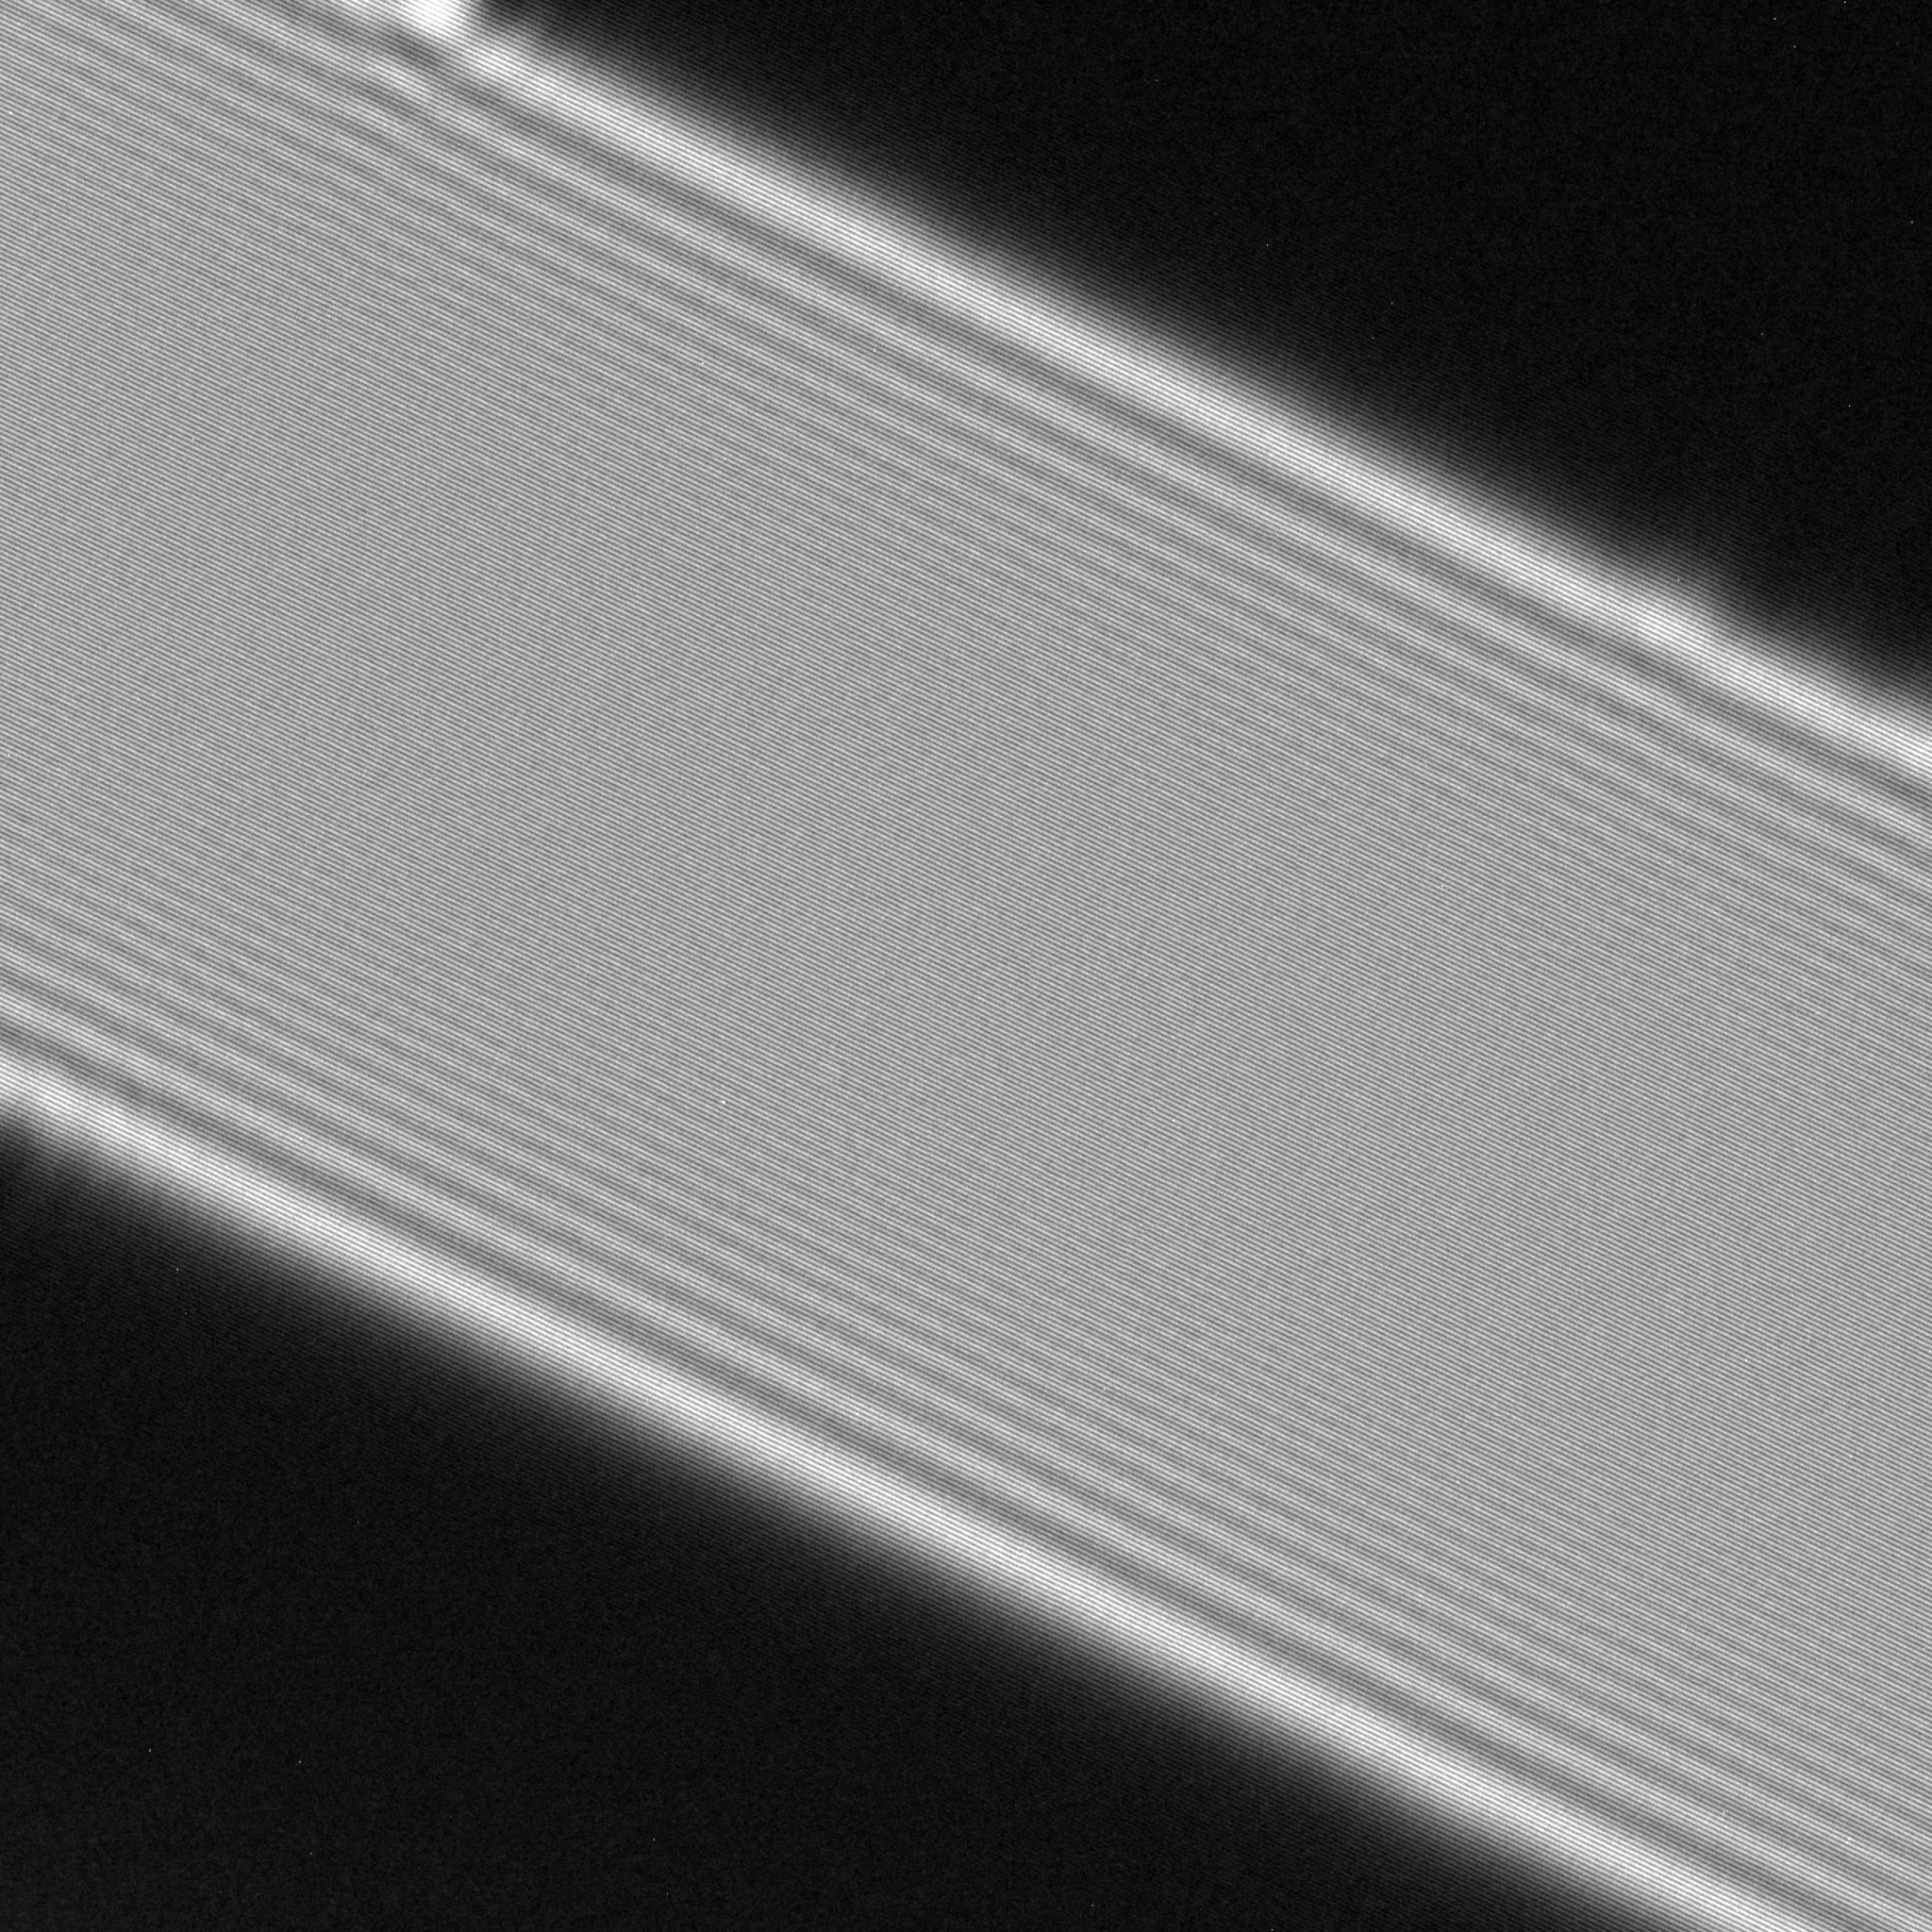
\includegraphics[width=\textwidth]{Gerüst/Abbildungen/Holographie/Probe/1_Leerhologramm_70.4V_Ltz_15500x.jpg}
         \caption{Leerhologramm}
         \label{P-NLeerEllip}
     \end{subfigure}
     \hfill
     \begin{subfigure}[b]{0.49\textwidth}
         \centering
         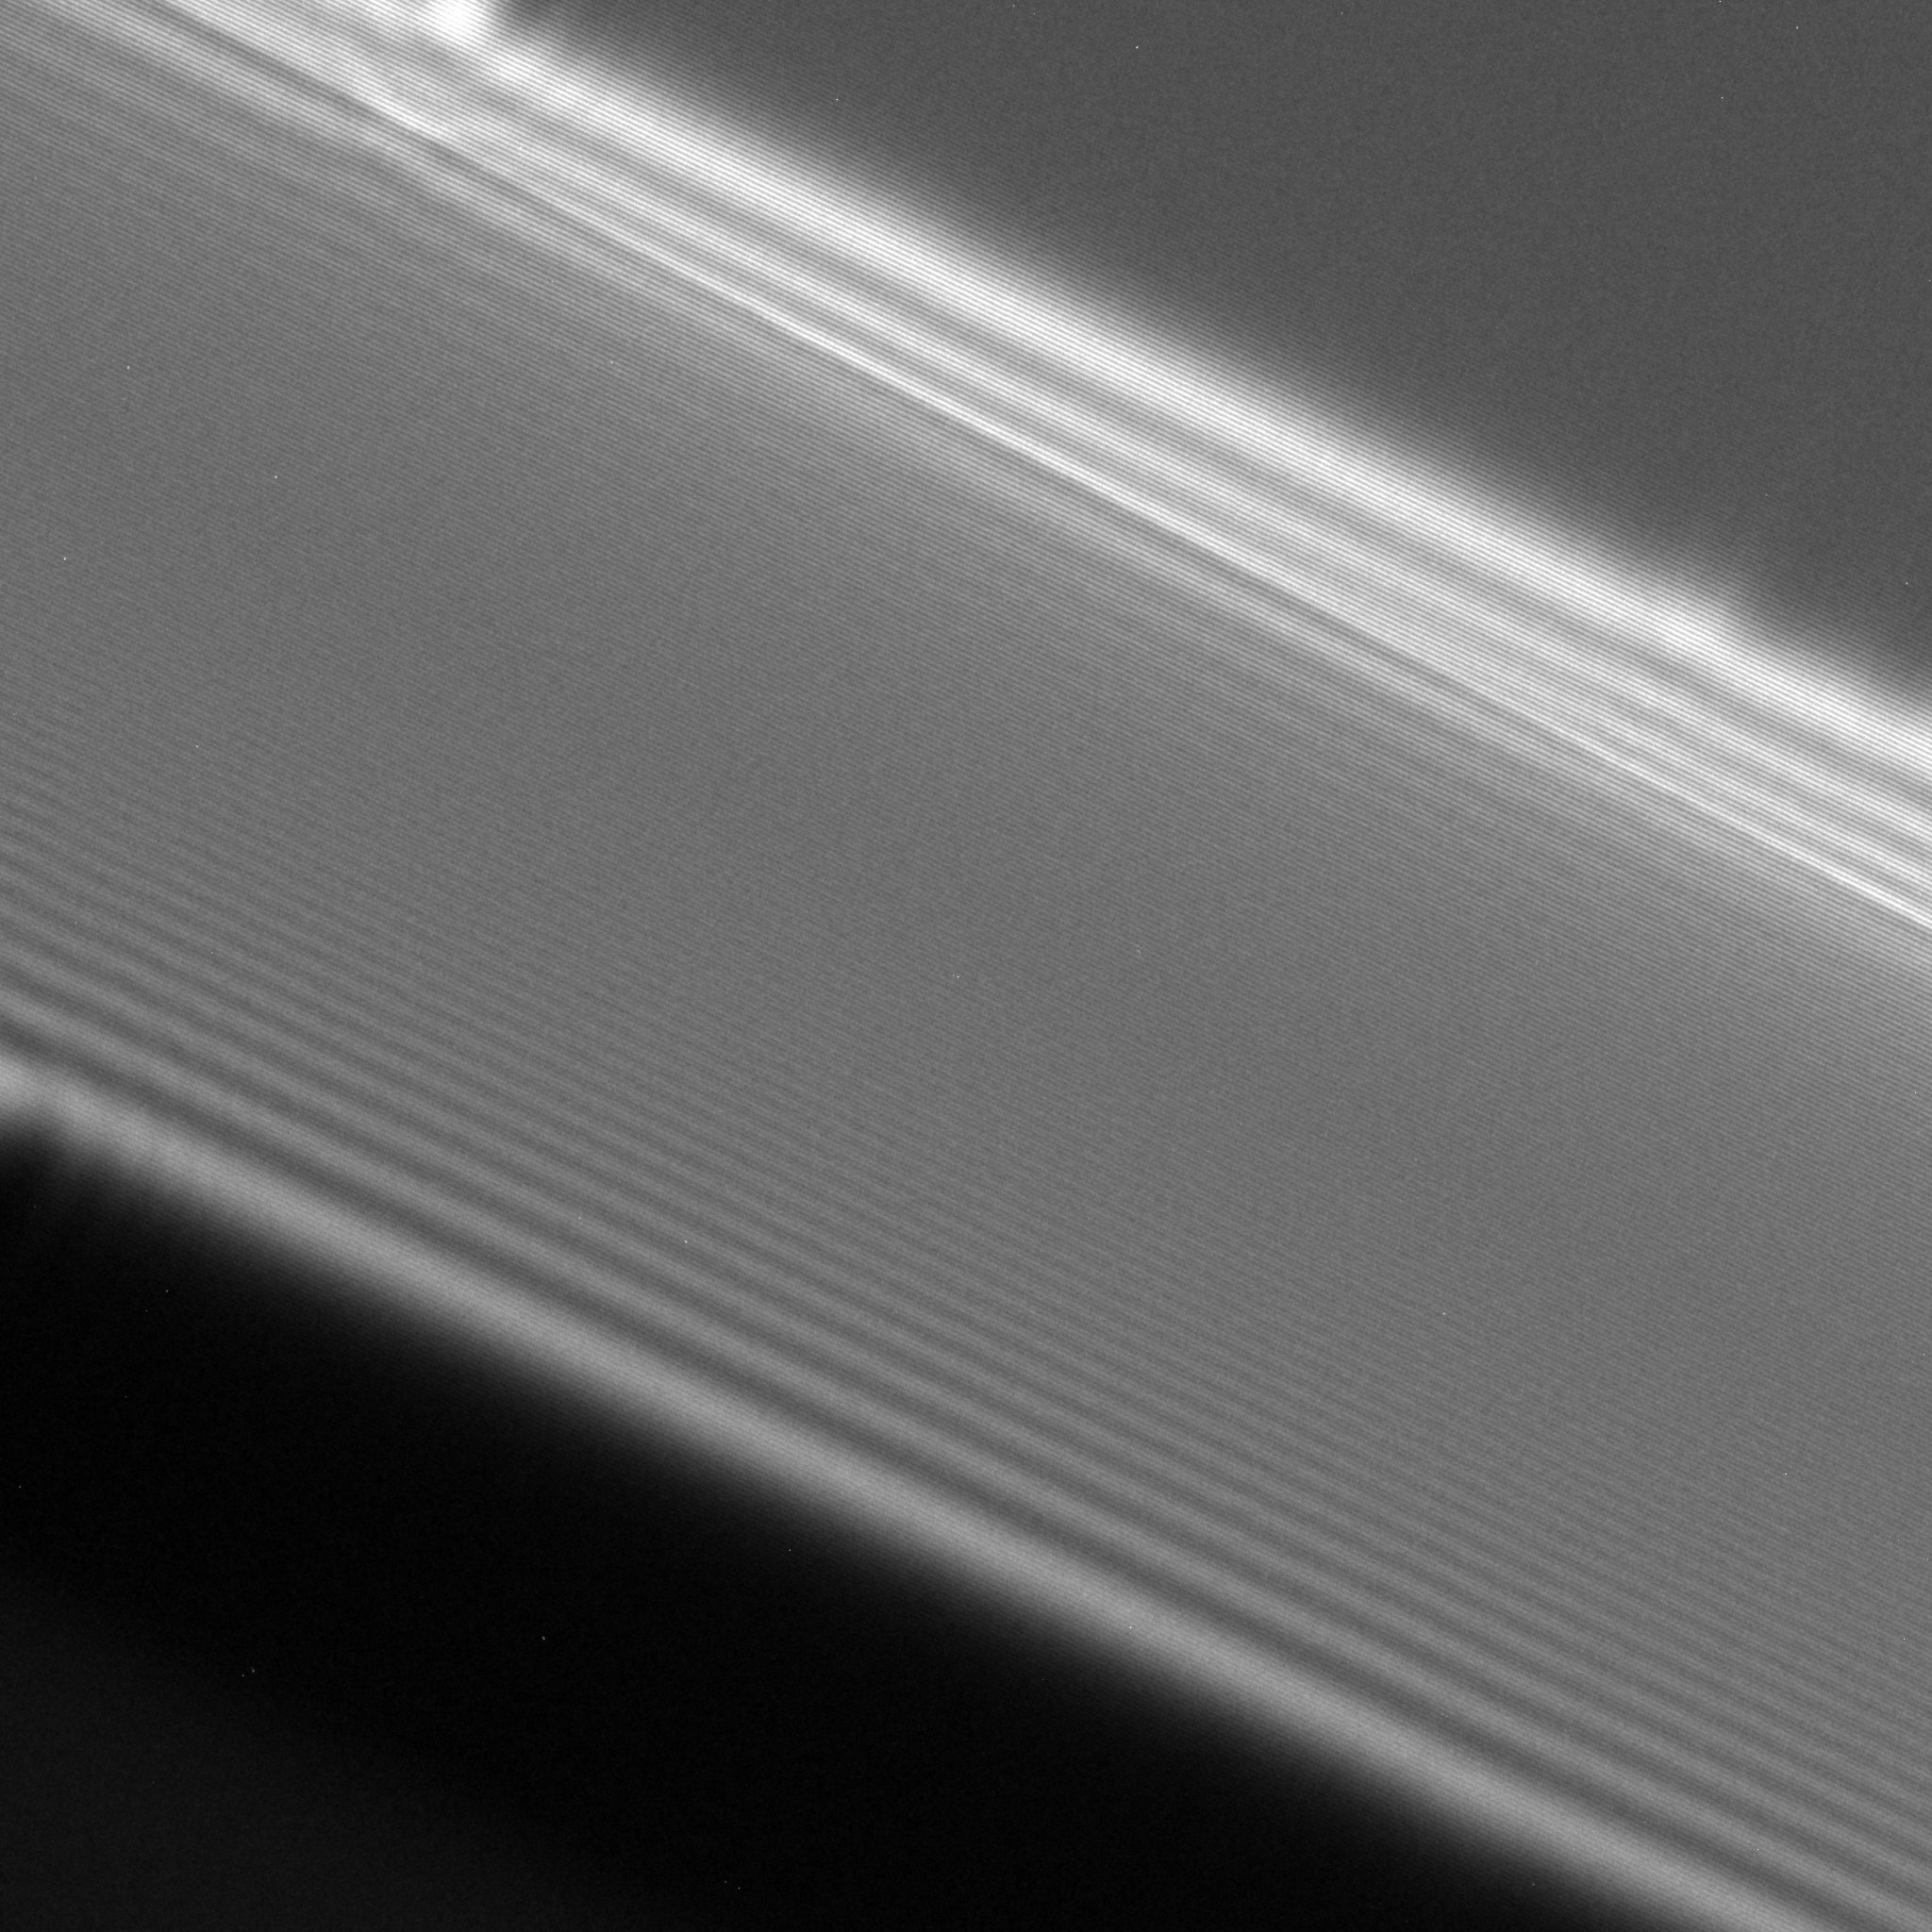
\includegraphics[width=\textwidth]{Gerüst/Abbildungen/Holographie/Probe/2_Probenhologramm_70.4V_Ltz_15500x.jpg}
         \caption{Objekthologramm}
         \label{P-NObjektEllip}
     \end{subfigure}
        \caption{Hologramm Aufnahme von Silikat Chip mit P-N Übergang mit Elliptischer Beleichtung}
        \label{P-NHologrammEllip}
\end{figure}

\begin{figure}
     \centering
     \begin{subfigure}[b]{0.3\textwidth}
         \centering
         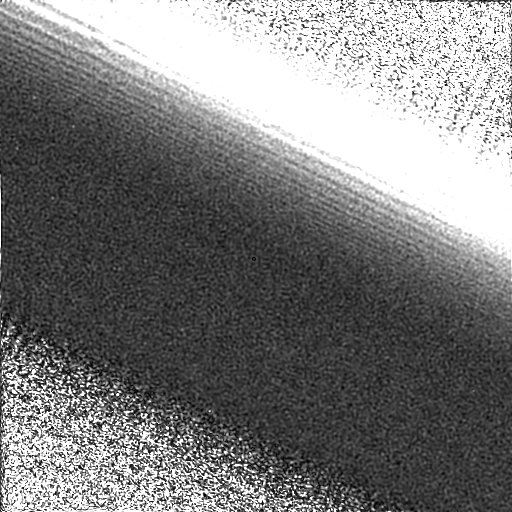
\includegraphics[width=\textwidth]{Holographie/Probe/3_Probenhologramm_70.4V_Ltz_15500x_iw_Amplitude.jpg}
         \caption{Amplitudenbild}
         \label{P-NAmpEllip}
     \end{subfigure}
     \hfill
     \begin{subfigure}[b]{0.3\textwidth}
         \centering
         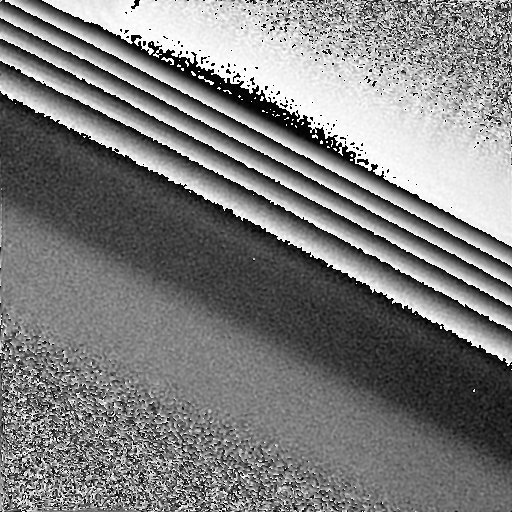
\includegraphics[width=\textwidth]{Holographie/Probe/5_Probenhologramm_70.4V_Ltz_15500x_iw_Phase_Wedge.jpg}
         \caption{Phasenbild, Wrapped}
         \label{P-NPhaseWEllip}
     \end{subfigure}
     \hfill
     \begin{subfigure}[b]{0.3\textwidth}
         \centering
         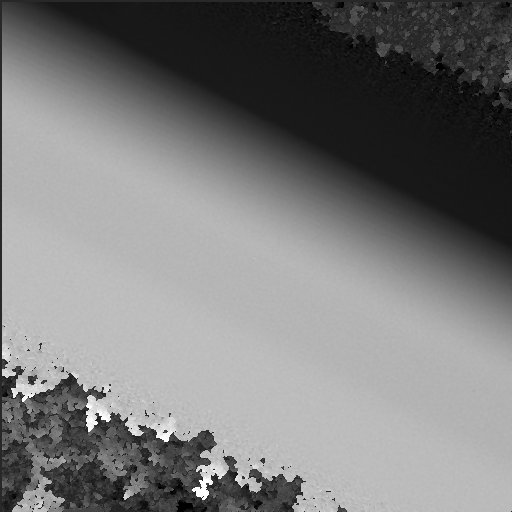
\includegraphics[width=\textwidth]{Holographie/Probe/6_Probenhologramm_70.4V_Ltz_15500x_iw_Phase_Wedge (unwrapped).jpg}
         \caption{Phasenbild, Unwrapped}
         \label{P-NphaseUEllip}
     \end{subfigure}
        \caption{}
        \label{AmpPhaseBildEllip}
\end{figure}
\section{STEM}

\subsection{STEM (Scanning transmission electron microscopy)}

STEM-Mikroskopie unterscheidet sich zur CTEM-Mikroskopie maßgeblich im Abbildungsmechanismus, während bei CTEM wie zuvor beschrieben eine Parallele Beleuchtung verwendet wird, die ein großen Bereich auf der Probe durchleuchtet, wird beim STEM ein Konvergenter Elektronenstrahl verwendet der nur eine fokussierten Prunkt im Objekt durchleuchtet. Dieser wird mit Hilfe von Ablenkmagneten über die Probe gerastert, um eine Aufnahme zu erstellen. Dieses Verfahren bietet einige Vorteile, wie eine hohe Auflösung, aber auch die Möglichkeit von einer Ortsaufgelösten Spektroskopie. Dabei können verfahren verwendet werden wie EELS (Electron Energy Loss Spectroscopy) oder EDX (Energy Dispersive X-ray). Außerdem kann ein Elementarer Z- Kontrast durch HAADF gemessen werden und ortsaufgelöst dargestellt werden.

\subsection{JEOL JEM-ARM300F2}
In diesem Versuchsteil wurde das „JEOL JEM-ARM300F2 STEM“ verwendet, dieses Mikroskop arbeitet mit einer Elektronen Beschleunigungsspannung von 60kV bis 300 kV mit einer Cold field emission gun. Dabei ist es in der Lage eine Ortsauflösung von ca. 53 pm zu erreichen.\\
Das Mikroskop ist mit einer CCD Kamera für CTEM ausgestattet, und HAADF, ADF, und BF Detektoren für die STEM Mikroskopie, zusätzlich verfügt es über eine EDX Messeinrichtung. Es ist Sonden-Korrigirtes Mikroskop, und komplett über den peripheren Computer bedient werden.

\subsection{BF (Brightfield)}
Beim Brightfield (BF) wird der Teil des Transmittierten Elektronenstrahl verwendet der direkt und ungestört durch das Objekt schralt. Der Brightfield Detektor befindet sich im Zentrum des transitierten strahlt. Solche Detektoren sind meist Halbleiter Detektoren und werden auch beim ADF und HAADF verwendet. \\
Der Kontrast wird dabei durch Absorption verursacht, diese entstehet durch Faktoren wie Kernladungszahl, die dicke des Objekts und Beugung im Objekt. Mit Hilfe von BF können z.B. hochauflösende Aufnahmen von leichten Atom Strukturen erstellt werden wie Sauerstoff erstellt werden.

\subsection{ADF (Annular dark-field)}
Bei der Annular Darkfield Mikroskopie werden die Elektronen des transmittierten Elektronenstrahles verwendet die vorwärts gestreut wurden, dabei werden die unterstreuten Elektronen nicht gemessen.  Ein ADF Detektor ist ringförmig so das lediglich die gestreuten Elektronen gemessen werden, die unterstreuten könne ungestört durch die Mitte des Detektors gelangen und für das BF oder EELS benutzt werden.  Beim ADF werden die elastisch durch Bragg-streuung gestreut Elektronen gemessen. Also an periodischen Strukturen die einer ähnlichen Periodizität aufweist wie die wellenlange des Elektronen Strahls, wie ist zum Beispiel in kristallen zu finden sind. 

\subsection{HAADF (High-angle annular dark-field)}
Bei der HAADF Mikroskopie werden die Elektronen des transmittierten Strahls gemessen die mit einem Großen Winkel gestreut wurden. Dabei werden die Elektronen am Atomkern durch die Rutherford Streuung gestreut, Die Streuung ist stark von der Kernzahl des Atoms abhängt. Der strak abhängige Kontrast des HAADF von der Kernzahl ermöglicht es eine ortsaufgeloste Verteilung von Schweren Elementen im Objekt darzustellen. Ein HAADF Detektor ist wie ein ADF Detektor ringförmig aufgebaut, jedoch ist das Loch im Zentrum wesentlich großer so das nur stark abgelenkte Elektronen gemessen werden.

\subsection{Ronchigram}
Ein Ronchigram ist ein Bild des Punktes im Unendlichem welches durch einen konvergenten Elektronenstahl an einer amorphen Struktur entstehet. Dabei ist der Fokus des Stahls genau auf der Probe so das eine unendliche Vergrößerung des Objektes entstehet. Ein Ronchigram kann Informationen über die Aberration des Mikroskops beinhalten und damit verwendet werden um diese zu korrigieren. Bei einem modernen Cs-Korrektor wird die Elektronensonde im STEM mit Hilfe des Ronchigram im Tableaux verwendet.

\subsection{STEM Versuch}
Um mit dem STEM Versuch zu beginnen, muss zuerst das JEOL Mikroskop Gecheckt, eingestellt und Korrigiert werden. Um das zu erreichen wurde wieder eine Standard Probe aus Gold Clustern und Latex Kugeln auf einem Kohlenstoff film verwendet. In der Mikroskop Software musste der Probenhalter auf dem die Probe montiert wurde ausgewählt werden, „Single Tilt“. Anschließend wurde die FEG vorbereitet und von Kontamination bereinigt, um eine maximale kohärente Beleuchtung zu erhalten. Dafür wurde die Quelle „Geflashed“, also stark erhitzt und eine Große Beschleunigungsspannung angelegt. Nachdem das Vakuum überprüft wurde \((5,6*10^{-6} mbar)\) und die Ventile geöffnet wurden, konnte die Elektronen Emission eingeschaltet werden und das Mikroskop im TEM Modus gestellt. An der CCD-Kamera wurden „Gain“ und „Offset“ eingestellt, damit das Bild einen guten Kontrast anzeigt.\\
Die Probe wurde in den Elektronenstrahl verfahren und eine geeignete Region auf der Probe identifiziert.\\
Das Mikroskop wurde nun in den STEM Modus gestellt, dafur wurde zunächst die Kamaralänge auf \(30cm\) vergrößert und eine \(CL_1\) Blende mit \(150\mu m\) eingefahren und die C1 Linse (spotsize) auf 7 gestellt.\\
Mit der CCD Kamera wurde nun das Ronchigram untersucht, dieses ist erreicht durch das Verfahren der Höhe, so dass die maximalle Unschärfe des Bildes erreicht wird. Anschließend wurde die Kamaralänge auf \(8cm\) gestellt und die STEM Detektoren BF, ADF HAADF herausgefahren um eine STEM Aufnahme zu erhalten, \cref{STEMAstigmatismus}.\\
Da in diesen aufnahmen das Mikroskop noch nicht korrigiert ist, ist in der DF Aufnahme ein deutliches Verschwimmen des Bildes in horizontaler
Richtung zu erkennen.\\
Diese Bildfehler sind überwiegen der Koma und Astigmatismus welche nun am Mikroskop korrigiert werden. Dies last sich grob mit Hilfe des Ronchigram erreichen.

\begin{figure}[H]
     \centering
     \begin{subfigure}[b]{0.49\textwidth}
         \centering
         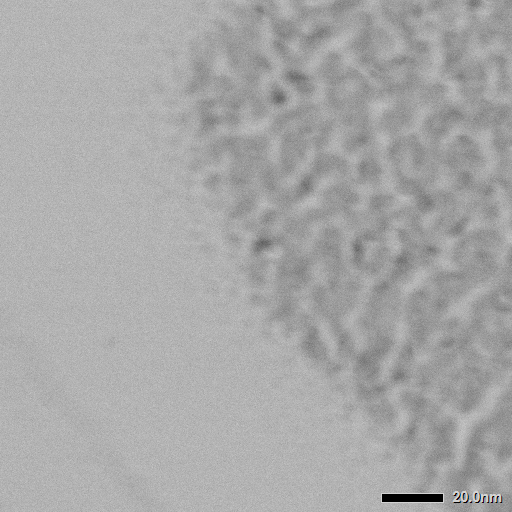
\includegraphics[width=\textwidth]{Gerüst/Abbildungen/STEM/STEM__20220817_1033_41_BF_ImagePanel3.png}
         \caption{BF}
         \label{astigBF}
     \end{subfigure}
     \hfill
     \begin{subfigure}[b]{0.49\textwidth}
         \centering
         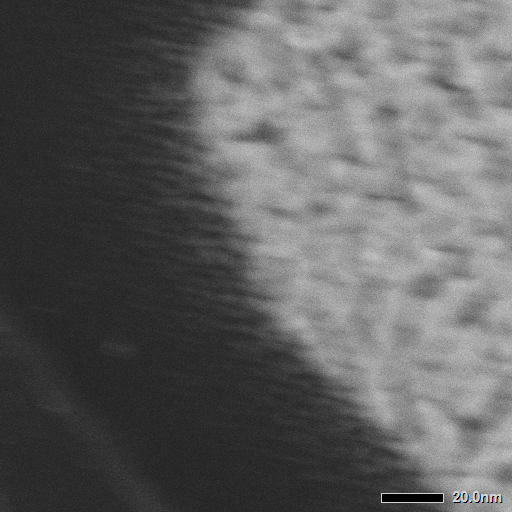
\includegraphics[width=\textwidth]{Gerüst/Abbildungen/STEM/STEM__20220817_1033_41_ADF1_ImagePanel1.png}
         \caption{HAADF}
         \label{astigDF}
     \end{subfigure}
        \caption{Unkorrigierte STEM Aufnahme von Au/Latex Probe}
        \label{STEMAstigmatismus}
\end{figure}

Zuerst wird mit dem Stigmator das Ronchigram so verzerrt das es symmetrisch ist und kleine Verzerrung in die X-/Y-Achse mehr erkennbar ist. Wenn man dann durch den Fokus wandert und die beiden Fokusse der Achsen an demselben Punkt sind, ist der Astigmatismus grob korrigiert. Später wird der restliche Fehler mit Hilfe der Mikroskop Software korrigiert.\\
Der Axiale Koma wird durch das verkippen des Strahles erreicht, dabei wird wieder durch den Fokus gefahren und so lange eingestellt bis das Bild symmetrisch durch den Fokus durchwandert. Die unendliche Vergrößerung ist dabei in der Mitte des Ronchigram. Diese Einstellungen wurden anschließend als Euzentrischer Fokus gespeichert. Das Korrigierte Ronchigram ist in der Aufnahme \cref{KorrRonchi} zu sehen, welches ausrechend verzerrungsfrei ist. Mit hilfe der Cs-Korrector software des mikroskops wurde der restliche Aberration gemessen und korrigiert. Die übrige Aberration nach deinem wiederholtem messen betrug: \(\zeta X: -0,2856 , Y: 0,4865 \).


\begin{figure}[H]
     \centering
  
         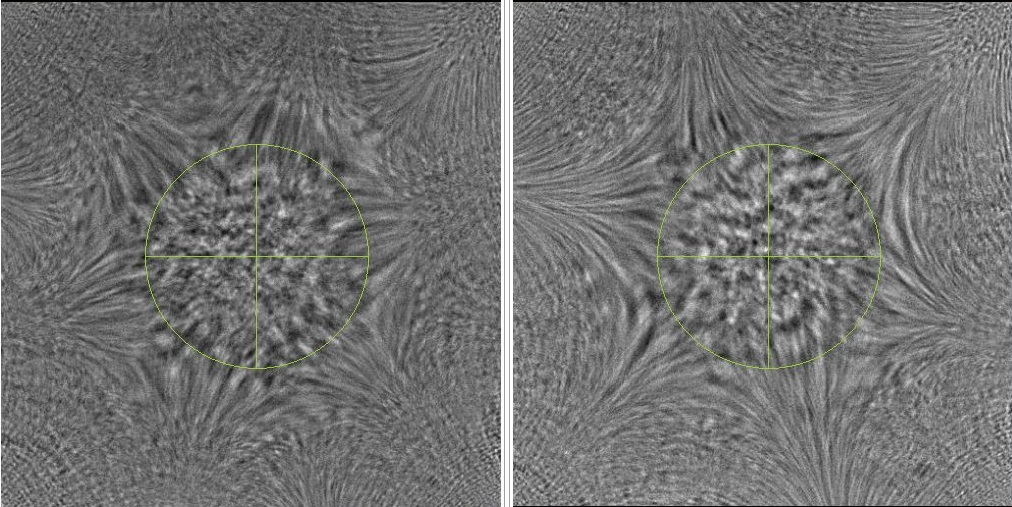
\includegraphics[width=\textwidth]{Gerüst/Abbildungen/STEM/corectors.jpg}
         \caption{Ronchigram im Über-/Underfokus nach der Aberration Korrektur}
         \label{KorrRonchi}

\end{figure}
Nach der Korrektur wurde eine Bildfehlerkorrigierte Aufnahmen im STEM Modus erstellt. Dabei wurde jedoch eine 30 µm \(Cl_2\) blende verwendet, die Abbildung \cref{STEMGold} zeigt die Goldcluster und Latex Kugeln. 
\begin{figure}
     \centering
     \begin{subfigure}[b]{0.3\textwidth}
         \centering
         \includegraphics[width=\textwidth]{Gerüst/Abbildungen/STEM/STEM__20220817_1123_03_BF_ImagePanel3.png}
         \caption{BF}
         \label{STEMGoldBF}
     \end{subfigure}
     \hfill
     \begin{subfigure}[b]{0.3\textwidth}
         \centering
         \includegraphics[width=\textwidth]{Gerüst/Abbildungen/STEM/STEM__20220817_1123_03_ABF_ImagePanel2.png}
         \caption{ADF}
         \label{STEMGoldADF}
     \end{subfigure}
     \hfill
     \begin{subfigure}[b]{0.3\textwidth}
         \centering
         \includegraphics[width=\textwidth]{Gerüst/Abbildungen/STEM/STEM__20220817_1123_03_ADF1_ImagePanel1.png}
         \caption{HAADF}
         \label{STEMGoldHAADF}
     \end{subfigure}
        \caption{STEM Aufnahme der Standard Probe. Mit Gold Cluster in verschiedenen Orientierungen und Kohlefilm (Mitte Links)}
        \label{STEMGold}
\end{figure}
Es sind klar die reihenartige Anordnung der Goldatome in den Gold Cluster erkennbar, jedoch mit unterschiedliche orientierten Goldatome Domänen.\\
Der Kontrast unterscheidet sich erwartungsgemäß ebenfalls. So ist in \cref{STEMGoldHAADF} der Bereich des Kohlefilms dunkler abgebildet, was an der geringen Kernladungszahl des Kohlenstoffes liegt und Beugung an diesen Strukturen daher unter kleineren Winkeln stattfindet. Die Goldkluster hingegen mit hoher Kernladungszahl, bieten dagegen einen starken Kontrast.

\subsection{Eigene Probe}
Es wurde nun die Standard Gold/Latex Probe mit der selbst erstellten Probe eines Silizium Wafer getauscht, dieser Prozess ist zu einem großen Teil analog zum Proben Tauschen beim TITAN Mikroskop und die neue Einstellung und Korrektur ist analog zum vorher beschriebenen Prozess. Dieser Prozess ist unten nur in Stichpunkten zusammengefast:
\begin{itemize}
 \item Probenhalter Auswechseln.
 \item Check Vakuum
 \item Beam öffnen (Ventile)
 \item In „Low Mag“ Wechseln 
 \item Probe Verfahren, Loch mit Kante finden
 \item In STEM Modus wechseln
 \begin{itemize}
   \item Detektoren auswählen, ADF1, BF, HAADF
 \end{itemize}  
 \item Kamera Länge wechseln -> 8 cm
 \item Am Detektor dem Kontrast und Brightness neu einstellen
 \item Ins Rochigramm wechseln
 \item Kamera Länge auf 30 cm Wechseln
 \item CCD-Kamara Einfahren 
 \item Amorphen Bereich nahe der Kante suche
 \item Proben Höhe verstellen so das im Ronchigramm in Fokus ist.
 \item Vergrößerung 1M
 \item Astigmatismus korrigieren 
 \item Stigmatoren einstellen
 \begin{itemize}
   \item Inneren Bereich im Ronchigram möglichst groß 
 \end{itemize}  
 \item Astigmatismus Nachkorrigieren
 \item Probenstelle finden
 \item Im Substrat (Kristall) ist die Kikutchi Linien durch verkippen orientieren
 \item Probenhöhe anpassen
 \begin{itemize}
   \item Standard Fokus + Z Höhe
   \item Im maximalen Fokus
 \end{itemize}
 \item Blende Cl2 30 µm einfahren
 \begin{itemize}
  \item Blende zentrieren
 \end{itemize}
 \item Zurück zu den Sensoren Wechseln
 \item Kameralänge auf 6 cm
\end{itemize}

Es wurden von Vier stellen der Probe STEM aufnahmen erstellt, mit dem Ziel eine geeignete Stelle zu finden um die anschließende EDX Messungen durchzuführen.\\
Die erste Aufnahme Zeit eine Übersichtsaufnehme, es ist die Klebe stelle zwischen den beiden Wafer an welcher die Ionen Dünnung das Loch erstellt hat. In der Aufnahme sind beide Wafer Seiten zu sehen, es sind außerdem leiterbahnen, Transistoren und andere Mikrochip Elemente zu sehen, da sie einen sehr guten Kontrast im Bf und DF bieten. Es ist außerdem zu erkennen das die Probe an einigen Stellen sehr dünn ist da teilweise nur Teile der leiterbahnen noch frei im Vakuum stehen, wahren bei der Ionen Dünnung das umgebende Silizium entfernt wurde, \cref{STEMEigeneProbeUebersicht}
\begin{figure}[H]
     \centering
     \begin{subfigure}[b]{0.49\textwidth}
         \centering
         \includegraphics[width=\textwidth]{Gerüst/Abbildungen/STEM/EigeneProbeBFUebersicht.jpeg}
         \caption{BF}
         \label{UeberBF}
     \end{subfigure}
     \hfill
     \begin{subfigure}[b]{0.49\textwidth}
         \centering
         \includegraphics[width=\textwidth]{Gerüst/Abbildungen/STEM/EigeneProbeHAADFUebersicht.jpeg}
         \caption{HAADF}
         \label{UeberDF}
     \end{subfigure}
        \caption{STEM Übersichtsaufnahme der eigenen Probe}
        \label{STEMEigeneProbeUebersicht}
\end{figure}
In der zweiten Aufnahme \cref{Pos1} ist eine leiterbahn zu sehen, mit denselben Bauteilen wie in der Übersicht Aufnahme außerdem ist ein größerer Teil des Silizium Volumen abgebildet, dort sind im BF mehrere Biegekonturen zu sehen.\\
In der dritten Aufnahme ist die leiterbahn mit unterschiedlichen Halbleiter Elementen zusehen. Hier wurde eine Größere Vergrößerung verwendet, diese Aufnahme ist von Oberen linken Rand des Loches, \cref{Pos2}.\\
Die vierte Aufnahme ist vom derselben leiterbahn am unter linken Ende des Lochs.  Die Probe ist hier etwas dicker als an der oberen Seite des Lochs, \cref{Pos3}.\\
Das fünfte Bild wurde von der rechten unteren Seite des Lochs erstellt, die Probe ist hier ziemlich dünn und weist eine der uniforme dicke auf, \cref{Pos4}.\\ 
Dieser Stelle der Probe wird anschließend für die EDX Messungen verwendet. Die Durchstahlbarkeit ist an dieser stell ist sehr gut, dies ist im BF Image gut erkennbar da die gesamte Probe hell beleuchtet wird, vom Vakuum bis zur dickste Stelle weit vom lock entfernt.\\
Die ADF und HAADF Bilder (\cref{Pos4ADF} und \cref{Pos4HAADF}) liefert auch einen sehr guten Kontrast welches auf die Kristallstruktur und gut unterscheidbaren Z werte deutet.  Es ist zusätzlich zu erkennen das die an der dünneren stellen der Probe i.e. nahe des loch, die Aufnahme heller ist. Also mehr gestreute Elektronen in der Lage sind dem Volumen zu entkommen und gemessen werden. Außerdem ist eine Beugungskontur nahe der Kante erkennbar.



\begin{figure}[H]
     \centering
     \begin{subfigure}[b]{0.4\textwidth}
         \centering
         \includegraphics[width=\textwidth]{Gerüst/Abbildungen/STEM/EigeneProbeBFPos1.jpeg}
         \caption{Position 1}
         \label{Pos1}
     \end{subfigure}
     \hfill
     \begin{subfigure}[b]{0.4\textwidth}
         \centering
         \includegraphics[width=\textwidth]{Gerüst/Abbildungen/STEM/EigeneProbeBFPos2.jpeg}
         \caption{Position 2}
         \label{Pos2}
     \end{subfigure}
      
 %\vspace{}

 \centering
     \begin{subfigure}[b]{0.4\textwidth}
         \centering
         \includegraphics[width=\textwidth]{Gerüst/Abbildungen/STEM/EigeneProbeBFPos3.jpeg}
         \caption{Position 3}
         \label{Pos3}
     \end{subfigure}
     \hfill
     \begin{subfigure}[b]{0.4\textwidth}
         \centering
         \includegraphics[width=\textwidth]{Gerüst/Abbildungen/STEM/EigeneProbeBFPos4.jpeg}
         \caption{Position 4}
         \label{Pos4}
     \end{subfigure}
     
      \centering
     \begin{subfigure}[b]{0.4\textwidth}
         \centering
         \includegraphics[width=\textwidth]{Gerüst/Abbildungen/STEM/EigeneProbeBFPos4ADF.jpeg}
         \caption{Position 4, ADF}
         \label{Pos4ADF}
     \end{subfigure}
     \hfill
     \begin{subfigure}[b]{0.4\textwidth}
         \centering
         \includegraphics[width=\textwidth]{Gerüst/Abbildungen/STEM/EigeneProbeBFPos4HAADF.jpeg}
         \caption{Position 4, HAADF}
         \label{Pos4HAADF}
     \end{subfigure}
     
     \caption{BF aufnahmen an Vier Verschiedenen Positionen an der eigenen Probe, ADF und HAADF Aufnahmen an der Position 4}
        \label{EigeneProbeBFPositionen}
 
\end{figure}

\section{STEM-EDX}
\subsection{EDX (energy dispersive X-ray)}
Beim EDX wird die Charakteristische Röntgenstrahlung gemessen die bei der Anregung des Atoms durch den Elektronenstrahl entsteht. Die Charakteristik Röntgenstrahlung entsteht, wenn ein hoch energetisches Anregungselektron ein innerschalen Elektron herausschlägt. Anschließend wird das entstandene Elektronenloch durch ein höherschaliges Elektron gefühlt, dabei wird ein hochenergetisches röntgen Photon freigesetzt. Dieses Photon entspricht der Energie Differenz der involvierten Schalen und ist damit charakteristisch für das Atom und die Energieschalen, so das ein Element eindeutig identifizierbar ist.\\
Bei der Anregung durch hoch energetische Elektronen wird zusätzlich Bremsstrahlung freigesetzt welche allerdings nicht charakteristisch für das Element ist. \\
In EDX Messungen werden zusätzlich charakteristische Strahlung von dem umgebenden Mikroskop: Probenhalter, Linse, Elektronenquelle etc. durch sekundäre Prozesse freigesetzt. Diese Störsignale werden auch gemessen und müssen in der Auswertung berücksichtigt werden.
Ein EDX Detektor wird heutzutage meistens mit einem SDD (Silicon Drift Detektor) betrieben, dieser ist aus einem Halbleiter gefertigt welcher die Energie eines Röntgenphotons misst indem er die Ionisation im Halbleiter durch das Photon misst. Dabei sind P gedopte Übergänge auf der oberflache des Detektors angebracht, wenn die Strahlung im Volumen des Detektors ionisiert wird driften anschließend die freigesetzten Elektronen zu einer Anode. Die dabei entstehende Ladung an der Anode kann anschließen gemessen und ausgewertet werden um die Energie des Photons zu bestimmen. Es muss jedoch darauf geachtet werden das die Intensität auf dem Detektor nicht zu groß ist da zwei Photonen die zeitlich sehr dicht beieinander den Detektor treffen zusammen gemessen werden können und sich dadurch die gemessene Energie der beiden Photonen addieren. (PileUp-Effekte).\\
Mit Hilfe des EDX kann eine Hoch aufgelöste elementare Verteilung in der Probe erstellt werden.

\subsection{STEM-EDX Versuch}
In diesem Teil war das Ziel ein EDX Mapping von dem zuvor ausgewählten Proben Region zu erstellen. Da wie zuvor erwähnt das Mikroskop selbst einen relevante Background Röntgenstrahlung produziert, muss diese in der Analyse berücksichtigt werden. Dafür wurde zuerst eine Background Aufnahme erstellt in der die Probe aus dem Elektronen strahl entfernt wird und ausschließlich Vakuum gemessen wird. In Aufnahme \cref{EDXSpecBG} ist das gemessen Spektrum zu sehen. In diesem Spektrum konnten die Peaks vom:  C, O, Fe, N Al, Au, Mo, Ti, W, Co und Cu gemessen werden. Einige dieser Peaks sind mit Kontamination zu erklären, z.B. C, N und O. Andere sind von Bauteilen des Mikroskops, wie Linsenpolschuhe, Magnetspulen, etc., diese Peaks sind von: Fe, Al, Ti, Co und Cu. Von Strahlenschutz Beschichtungen sind zum Beispiel die Ag Peaks. Die W Peaks sind durch Kontaminirung FETs zu erklären, sogenante Tungsten-Plays.

\begin{figure}[H]
     \centering
     \begin{subfigure}[b]{0.49\textwidth}
         \centering
         \includegraphics[width=\textwidth]{Gerüst/Abbildungen/EDX/SpektrumBackground.jpg}
         \caption{Background}
         \label{EDXSpecBG}
     \end{subfigure}
     \hfill
     \begin{subfigure}[b]{0.49\textwidth}
         \centering
         \includegraphics[width=\textwidth]{Gerüst/Abbildungen/EDX/Spektrum.jpg}
         \caption{Probe}
         \label{EDXSpecProb}
     \end{subfigure}
        \caption{EDX Spektrum Aufnahmen der Hintergrunds Strahlung und der der Eigenen Si Probe}
        \label{EDX}
\end{figure}

Anschließend wurde die Probe wieder an die vorherige Position eingefahren und eine EDX-Aufnahme erstellt. Das Resultierende Spektrum ist in Abbildung \cref{EDXSpecProb} zu sehen. In diesem sind die N, F, O, Al und Co Starker ausgeprägt und zusätzlich ist die Si Peaks abgebildet.\\
Der Kohlenstoff auf der Probe ist mit hoher Wahrscheinlichkeit durch Kontamination entstanden. Da es ziemlich gleichmäßig auf der gesamten Probe erkennbar ist, außerdem ist er starker in dem hohen Kontrast Bereichen abgebildet, in den vor allem Metalle gemessen werden wie Al, W und Ti. Die Vermutung liegt nahe das dieser Starke C Kontrast durch Bremsstrahlung und sekundäre Effekte erzeugt wird welche unterstutzt wird mit der Kohlenstoff Abbildung bei der die Bremsstrahlung abgezogen wurde. Dort ist die Verteilung über die gesamte Probe sehr viel homogener, \cref{EDXC}.

\begin{figure}[H]
     \centering
     \begin{subfigure}[b]{0.49\textwidth}
         \centering
         \includegraphics[width=\textwidth]{Gerüst/Abbildungen/EDX/OhneSystemPeaks C K.jpg}
         \caption{Mit Bremsstrahlung}
         \label{EDXCmBS}
     \end{subfigure}
     \hfill
     \begin{subfigure}[b]{0.49\textwidth}
         \centering
         \includegraphics[width=\textwidth]{Gerüst/Abbildungen/EDX/QuantAnalyse_ohneBremsstrahlung C K.jpg}
         \caption{Ohne Bremsstrahlung}
         \label{EDXCoBS}
     \end{subfigure}
        \caption{EDX Map von Kohlenstoff mit und ohne Bremsstrahlung}
        \label{EDXC}
\end{figure}

Sauerstoff ist auf der Probe auch recht homogen verteil, jedoch sind sehr klare Strukturen von Sauerstoff armen/leeren Regionen zu sehen, \cref{EDXO}. Die Sauerstoff verarmten Zonen sind vor allem an Mikrochip Elementen die Metalle aufweisen wie Al, Ti enthalten, diese sind wahrscheinlich die leiterbahnen und Transistoren. Außerdem ist im Volumen des Chips (hinter der letzten leiterbahn, rechts), kein Sauerstoff vorhanden. In der Si Aufnahme \cref{EDXSi} ist auch zu erkennen, dass das eine reine Silizium Region ist, wahrscheinlich der ursprüngliche Wafer aus einem perfekten Silizium Chip bevor er weiterverarbeitet wurde. Der Sauerstoff ist möglicherweise auf die Probe bei der Verbreitung des Wafers gekommen, vielleicht bei lithographischen Prozessen, ob es eine Verunreinigung oder systemrelevant ist kann nicht beantwortet werden.

\begin{figure}
     \centering
     \begin{subfigure}[b]{0.3\textwidth}
         \centering
         \includegraphics[width=\textwidth]{Gerüst/Abbildungen/EDX/QuantAnalyse_ohneBremsstrahlung O K.jpg}
         \caption{O}
         \label{EDXO}
     \end{subfigure}
     \hfill
     \begin{subfigure}[b]{0.3\textwidth}
         \centering
         \includegraphics[width=\textwidth]{Gerüst/Abbildungen/EDX/QuantAnalyse_ohneBremsstrahlung Si K.jpg}
         \caption{Si}
         \label{EDXSi}
     \end{subfigure}
     \hfill
     \begin{subfigure}[b]{0.3\textwidth}
         \centering
         \includegraphics[width=\textwidth]{Gerüst/Abbildungen/EDX/QuantAnalyse_ohneBremsstrahlung Al K.jpg}
         \caption{Al}
         \label{EDXAl}
     \end{subfigure}
        \caption{EDX Maps von Sauerstoff, Silikat und Aluminium, ohne Bremsstrahlung}
        \label{EDXCSiAl}
\end{figure}

Das Aluminium auf der Probe ist ausschließlich in den leiterbahnen verwendet worden, es hat einen sehr starken Kontrast und diese Regionen werden in den anderen EDX Element Mapps leer (dunkel) dargestellt, \cref{EDXAl}.


\begin{figure}[H]
     \centering
     \begin{subfigure}[b]{0.49\textwidth}
         \centering
         \includegraphics[width=\textwidth]{Gerüst/Abbildungen/EDX/Overlay(Si_N_Ti) OVERLAY.jpg}
         \caption{Si:B, N:G, Ti:R}
         \label{Overlay}
     \end{subfigure}
     \hfill
     \begin{subfigure}[b]{0.49\textwidth}
         \centering
         \includegraphics[width=\textwidth]{Gerüst/Abbildungen/EDX/Overlay(Ti_Si_N) OVERLAY.jpg}
         \caption{Ti:B Si:G, N:R}
         \label{Overlay2}
     \end{subfigure}
        \caption{EDX Map Overlay der Eigen Probe von Titan, Silikat und Stickstoff}
        \label{EDXOverlay}
\end{figure}

Die besonderes Spannenden Mapps sind die der Ti, Si und N, um diese besser zu verstehen und zuzuordnen sind sie am besten in den beiden Overlay aufnahmen \cref{EDXOverlay} dargestellt, hier kann man einen sehr guten N Kontrast am der rechten Seiter des linken Al leiterband sehen, und an den Rändern der anderen Leitungsbahnen. Was das N an diesen Stellen bewirkt kann nicht gesagt werden aber es scheint für den Übergang zwischen Si und Al relevant zu sein. Das Titan scheint eine Rolle für das dopen des Si zu spielen, es ist an den Al Leiterband Übergängen zu sehen, aber auch an eigenen leiterbahnen die die AL bahnen verbinden. Es ist zusätzlich ein leichter Kontrast im Si an der linken Al leiterbahn zu sehen, es wird vermutet das diese die Transistoren sind, aber eine Bestimmung ist aus Mengel an Wissen über Halbleiter und Mikrochips nicht möglich.


%\input{STEM-EDX}
%\section{Zusammenfassung}



\begin{thebibliography}{xx}


\bibitem[1]{1}
K. Arts, H. Thepass, M. A. Verheijen, R. L. Puurunen, W. M. M. Kessels, and H. C. M. Knoops, Chemistry of materials : a publication of the American Chemical Society 33, 13 (2021).
\bibitem[2]{2}
 M. L. Lehmann, EM 1&2: Elektronenmikroskopie 1 & 2: Vorlesungen und Presenationen (Berlin, 2021).
\bibitem[3]{3}
Dirk Berger ZELMI (2022).
\bibitem[4]{4}
Dirk Berger ZELMI (2022).
\bibitem[5]{5}
Tore Niermann and Juan Bettinelli (2022).
\bibitem[6]{6}
J. Bettinelli, Probenprepation Messdatenprotokoll TEM-Labor (2022).
\bibitem[7]{7}
J. Bettinelli, TEM proben Vorbereitung 1,2&3 Mitschrift (2022).
\bibitem[8]{8}
M. L. Lehmann, TEM-Laborpraktikum 2022 Aufgaben- und Zeitplan (2022).
\bibitem[9]{9}
Dirk Berger ZELMI, STEM-EDX Praktikum ZELMI 2022 07 25: Theorie STEM EDX (Berlin, 2022).
\bibitem[10]{10}
Frederik Otto, TEM column and TEM operation: TITAN Bedinung (Berlin, 2022).
\bibitem[11]{11}
Juan Bettinelli, Holographie Labor Mitschirft (2022), Holographie Labor Mitschirft. Accessed 1 November 2022.
\bibitem[11]{11}
Juan Bettinelli, TEM Beugung Labor Mitschrift (2022). Accessed 1 November 2022.
\bibitem[11]{11}
Juan Bettinelli, TEM Holographie Labor Mitschrift (2022). Accessed 1 November 2022.
\bibitem[12]{12}
S. Sören, Präparation von Proben für TEM-Untersuchungen: Präparation von Proben für TEM-Untersuchungen (Berlin, 2022).
\bibitem[13]{13}
T. Winkler, TEM Beugung Mitschrift 2 (2022). Accessed 16 November 2022.
\bibitem[14]{14}
Tolga, Holographie Tafel aufschrift (2022).
\bibitem[15]{15}
Juan Bettinelli and Till Winkle, STEM Labor Mitschrift Gruppe 5 Scan (2022).
\bibitem[16]{16}
TITAN and Frederik Otto, TITAN Ein/Ausscheck verfahren: TITAN Bedinung (Berlin, 2022). Accessed 1 November 2022.
\bibitem[17]{17}
Dirk Berger ZELMI, Theorie STEM-EDX 2022 06 20.pptx: Versuchsteil STEM-EDX (2022).
\bibitem[18]{18}
Frederik Otto, Beugung Tafel Foto (TU Berlin). Accessed 1 October 2022.




\end{thebibliography}% zum Verweis auf Items aus Literatur.tex verwendet: \cite{lit:paper}
% \section{Appendix}
\subsection{Appendix Tital}



\end{document}